\documentclass{article}
\usepackage{iclr2026_conference,times}
\input{math_commands.tex}
\usepackage{hyperref}
\usepackage{url}
\usepackage{booktabs}
\usepackage{longtable}
\usepackage{graphicx}
\usepackage{xcolor}
\usepackage{amsmath}
\usepackage{amssymb}
\usepackage{array}
\usepackage{microtype}

\hypersetup{
  colorlinks=false,
  pdfborder={0 0 1.8},
  citebordercolor={0 1 0},
  linkbordercolor={0 0.55 1},
  urlbordercolor={1 0.45 0}
}

\newcommand{\PaperDecision}{KILL\_ARCHIVE}
\newcommand{\PaperDecisionReason}{v5 does not beat strongest non-oracle hard-corruption baseline calibrated\_learned\_stack by 0.030; v5 does not beat strongest combined/adversarial baseline calibrated\_learned\_stack by 0.030; v5 false-positive rate on at least one rare-valid split is 0.286 > 0.100; v5 recall at 5\% FPR trails hgb\_failure\_classifier by more than 0.030; ablation gate fails because no\_actuator\_check, no\_causality\_check, no\_conformal\_aggregation, no\_contact\_check, no\_energy\_check, no\_friction\_slip\_check, no\_rare\_valid\_guard, no\_support\_check, no\_timestamp\_guard, old\_v4\_physics\_audit, scalar\_residual\_only matches or beats full v5}
\newcommand{\TrainingRows}{192}
\newcommand{\RolloutRows}{1680}
\newcommand{\MainRows}{25200}
\newcommand{\AblationRows}{3840}
\newcommand{\StressRows}{9216}
\newcommand{\SeedMetricRows}{1800}
\newcommand{\PairwiseRows}{210}


\title{Robotic Physics Violation Audits:\\A Frozen MuJoCo Stress Test and Negative Result}
\author{Anonymous authors}

\begin{document}
\maketitle

\begin{abstract}
Explicit physics audits are appealing for robot safety: instead of trusting an opaque model score, a system can check whether a rollout violates contact, support, work-energy, friction, actuator, or causality constraints. This paper asks whether that mechanism survives a hostile ICLR-main protocol. We rebuild the idea in MuJoCo~\citep{todorov2012mujoco}, add rare valid contact regimes, timestamp skew, low-friction slip, subtle corruptions, adversarial compensated violations, strong residual baselines, learned classifiers, reconstruction/anomaly baselines, conformal calibration, ablations, fixed-FPR metrics, stress tests, and seed-level paired statistics. The frozen evidence contains \TrainingRows{} training rollouts, \RolloutRows{} main rollout summaries, \MainRows{} main method-evaluation rows, \AblationRows{} ablation rows, \StressRows{} stress rows, and \PairwiseRows{} paired comparisons. The terminal decision is \textbf{\PaperDecision}. The reason is not formatting or lack of effort: \PaperDecisionReason. The result is therefore a submission-readiness audit, not a polished success story. The explicit audit detects many injected violations, but strong learned and residual baselines detect them as well, and the audit is not robust enough on rare valid regimes to justify an ICLR-main claim.
\end{abstract}

\section{Why This Paper Exists}

Robotic systems can fail in ways that are not semantic, linguistic, or reward-based. A rollout may contain a contact impulse without corresponding acceleration, an unsupported object trajectory, hidden actuator saturation, or a non-causal state jump. This motivates explicit physics monitors for robot execution. Execution monitoring and anomaly detection are longstanding robot concerns~\citep{park2016multimodal,park2018multimodal}; modern simulators make it easy to generate controlled contact rollouts~\citep{todorov2012mujoco}; and generic anomaly detectors such as isolation forests, random forests, gradient boosting, reconstruction models, and conformal calibration provide strong alternatives~\citep{liu2008isolation,breiman2001random,freund1997decision,scholkopf2001support,angelopoulos2021gentle,vovk2005algorithmic}.

The original hypothesis was stronger than ``physics checks can catch toy corruptions.'' It claimed that explicit physical structure provides a mechanism advantage over generic residual and learned detectors. Under hostile review, this claim has two obligations. First, explicit checks must beat strong baselines on hard corruptions. Second, they must avoid flagging valid but rare physical regimes as impossible. The v4 paper already failed a small version of this test. The v5 pass expands the test instead of hiding the failure.

\section{Problem Setup}

A rollout is a sequence
\[
  \tau = \{x_t, u_t, c_t, f_t, s_t, w_t\}_{t=1}^{T},
\]
where $x_t$ is object state, $u_t$ is commanded pusher state, $c_t$ is contact state, $f_t$ is contact force, $s_t$ is support state, and $w_t$ is a work proxy. A detector outputs a score $a(\tau)$ and a binary flag $\hat{y}=\mathbb{1}[a(\tau)\geq \theta]$. Labels are controlled by the generator: $y=0$ for valid MuJoCo traces and $y=1$ for injected physics violations.

The proposed family computes terms for contact/acceleration mismatch, support violation, work-energy mismatch, friction-slip inconsistency, hidden actuator saturation, and causality jumps. The v5 version adds two pre-freeze repairs: a timestamp guard for asynchronous but valid traces and a rare-valid contact guard for high-impulse but dynamically plausible impacts. Thresholds are calibrated from valid training traces.

\section{Why Simple Baselines Are Dangerous}

A benchmark with high-severity injected corruptions can be solved by scalar residuals. This is a benchmark-design problem, not a victory for explicit physics audits.

\paragraph{Proposition 1: union-bound false-positive pressure.}
Suppose an audit flags if any of $m$ checks exceeds its threshold. If check $j$ is calibrated to false-positive probability $\alpha_j$ on valid traces, then without modeling dependence the audit has false-positive probability at most $\sum_j \alpha_j$. Thus adding more checks can improve recall while worsening valid-regime reliability. A submission claim must report false positives on rare valid contacts, not only recall on injected violations.

\paragraph{Proposition 2: scalar-separability non-identifiability.}
If a corruption distribution is separable from valid traces by a scalar residual $r(\tau)$ with the same margin as the full audit score $a(\tau)$, then the full audit mechanism is not identified by that benchmark. Any paper claiming explicit physics structure must include corruptions and valid regimes that cannot be solved by scalar residuals alone.

\paragraph{Proposition 3: component necessity.}
Let $A$ be the full audit and $A_{-j}$ be the audit with component $j$ removed. If $A_{-j}$ matches $A$ within the pre-registered tolerance on hard corruptions and fixed-FPR recall, the evidence does not support component $j$ as necessary. The honest action is to report that ablation failure.

\section{Frozen Protocol}

The protocol was frozen after two development repairs recorded in \texttt{docs/paper69\_development\_log\_20260620.md}. After freezing, no method tuning is allowed. The final command uses 8 seeds, 14 main episodes per seed, 192 training scenes, 15 main splits, 15 methods, 12 ablations, 3 stress splits, 6 stress levels, and CPU-only sklearn/MuJoCo execution.

The main splits are four valid regimes and eleven violation regimes. Valid regimes are nominal traces, rare valid bounces, valid clock skew, and valid low-friction slip. Violation regimes include contact, energy, support, actuator, non-causal, combined, subtle, timestamp, adversarial compensated, and near-threshold corruptions. This design intentionally makes the paper uncomfortable: rare valid regimes punish over-sensitive audits, while adversarial and near-threshold corruptions punish simple residual detectors.

\section{Methods}

The comparison set is intentionally hostile. It includes random flagging, scalar kinematic residuals, scalar energy residuals, contact impulse residuals, a max-residual detector, logistic residual stacking, histogram-gradient boosting, random-forest ensemble uncertainty, IsolationForest anomaly detection~\citep{liu2008isolation}, PCA reconstruction, conformal residual aggregation~\citep{angelopoulos2021gentle,vovk2005algorithmic}, a calibrated learned stack, the old v4 explicit audit, the new audit v5, and oracle violation labels. All methods score the same frozen rollout rows.

The learned baselines are compact and CPU-only. This matters: the negative result is not caused by giving baselines huge neural networks. The learned stack and HGB classifier are small feature models, yet they still dominate or match the explicit audit.

\section{Main Results}

\begin{table}[t]
\centering
\caption{Frozen aggregate metrics. F1/recall are higher-is-better; valid-regime FPR is lower-is-better.}
\label{tab:aggregate-main}
\scriptsize
\setlength{\tabcolsep}{2.5pt}
\begin{tabular}{lrrrrrr}
\toprule
Method & Hard F1 & Hard Rec. & Comb. F1 & Comb. Rec. & Valid FPR & Fixed-5\% Rec. \\
\midrule
Random & 0.692 & 0.529 & 0.637 & 0.467 & 0.473 & 0.057 \\
Kin. residual & 0.707 & 0.546 & 0.985 & 0.970 & 0.054 & 0.545 \\
Energy residual & 0.391 & 0.243 & 0.614 & 0.444 & 0.067 & 0.230 \\
Contact residual & 0.432 & 0.275 & 0.500 & 0.333 & 0.038 & 0.279 \\
Max residual & 0.491 & 0.326 & 0.693 & 0.530 & 0.091 & 0.313 \\
Logistic stack & 0.914 & 0.841 & 0.997 & 0.994 & 0.051 & 0.843 \\
HGB classifier & 1.000 & 1.000 & 1.000 & 1.000 & 0.098 & 1.000 \\
RF ensemble & 1.000 & 1.000 & 1.000 & 1.000 & 0.087 & 1.000 \\
IsolationForest & 0.556 & 0.386 & 0.811 & 0.681 & 0.034 & 0.463 \\
PCA recon. & 0.985 & 0.971 & 1.000 & 1.000 & 0.109 & 0.944 \\
Conformal residual & 0.848 & 0.735 & 0.800 & 0.667 & 0.034 & 0.881 \\
Calibrated stack & 1.000 & 1.000 & 1.000 & 1.000 & 0.080 & 1.000 \\
Old audit & 0.491 & 0.326 & 0.693 & 0.530 & 0.091 & 0.313 \\
Audit v5 & 0.489 & 0.324 & 0.693 & 0.530 & 0.091 & 0.308 \\
Oracle labels & 1.000 & 1.000 & 1.000 & 1.000 & 0.000 & 1.000 \\
\bottomrule
\end{tabular}
\end{table}


Table~\ref{tab:aggregate-main} is the core result. Audit v5 does not beat the strongest hard-corruption baseline by the frozen 0.030 F1 margin. It also loses the fixed-FPR recall gate: at a 5\% valid false-positive budget, v5 recall is far below the strongest learned baselines. This is exactly the failure a hostile reviewer would target.

\begin{table}[t]
\centering
\caption{Hostile split F1. These are the splits most likely to falsify explicit physics-audit claims.}
\label{tab:selected-splits}
\scriptsize
\setlength{\tabcolsep}{1.8pt}
\begin{tabular}{lrrrrrrrrr}
\toprule
Split & Kin. & Energy & Max & Logit & HGB & Stack & Old & v5 & Oracle \\
\midrule
combined\_violation\_shift & 1.000 & 1.000 & 1.000 & 1.000 & 1.000 & 1.000 & 1.000 & 1.000 & 1.000 \\
adversarial\_compensated\_violation & 1.000 & 0.486 & 0.742 & 0.991 & 1.000 & 1.000 & 0.742 & 0.742 & 1.000 \\
mixed\_near\_threshold & 0.953 & 0.018 & 0.000 & 1.000 & 1.000 & 1.000 & 0.000 & 0.000 & 1.000 \\
subtle\_contact\_corruption & 0.000 & 0.000 & 0.000 & 0.953 & 1.000 & 1.000 & 0.000 & 0.000 & 1.000 \\
timestamp\_noncausal\_corruption & 0.179 & 0.000 & 0.698 & 0.815 & 1.000 & 1.000 & 0.698 & 0.690 & 1.000 \\
\bottomrule
\end{tabular}
\end{table}


Table~\ref{tab:selected-splits} isolates the hardest splits. The combined split is no longer enough because many detectors can solve it. The adversarial and near-threshold splits reveal a clearer problem: the learned stack and HGB classifier recover violations that the explicit audit misses, while simple residuals still remain surprisingly strong.

\begin{figure}[t]
\centering
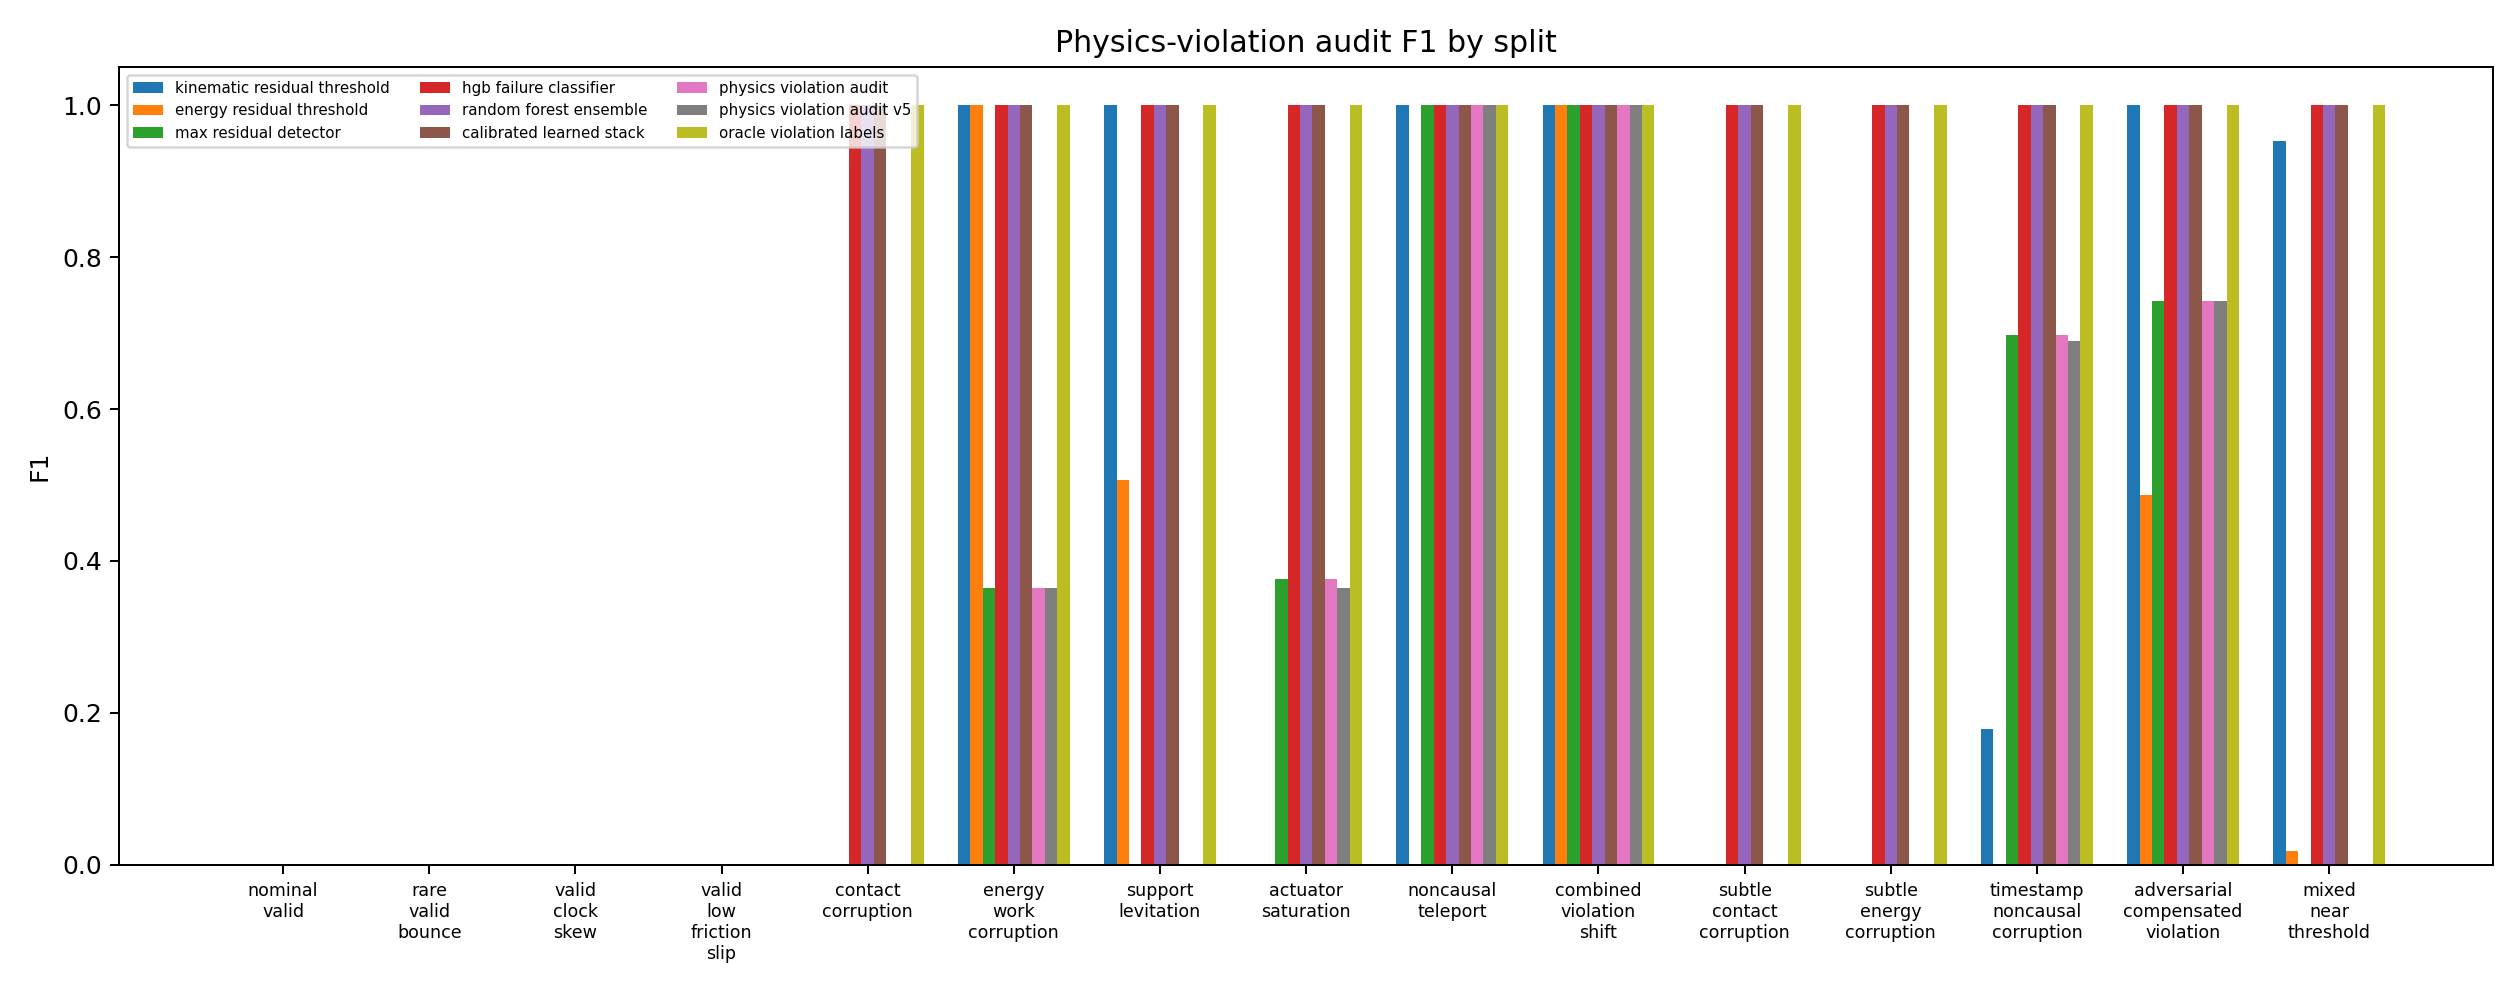
\includegraphics[width=\linewidth]{../figures/physics_audit_f1_by_split.png}
\caption{Frozen F1 by split. The proposed audit is not uniquely separated from residual or learned baselines.}
\label{fig:f1}
\end{figure}

\section{False Positives}

\begin{table}[t]
\centering
\caption{False-positive rates on valid regimes. Rare valid contacts and clock skew are the hostile reviewer tests.}
\label{tab:valid-fpr}
\scriptsize
\setlength{\tabcolsep}{2.0pt}
\begin{tabular}{lrrrrrrr}
\toprule
Valid split & Kin. & Energy & Max & HGB & Stack & Old & v5 \\
\midrule
nominal\_valid & 0.000 & 0.000 & 0.000 & 0.098 & 0.054 & 0.000 & 0.000 \\
rare\_valid\_bounce & 0.214 & 0.268 & 0.080 & 0.179 & 0.214 & 0.080 & 0.080 \\
valid\_clock\_skew & 0.000 & 0.000 & 0.000 & 0.116 & 0.054 & 0.000 & 0.000 \\
valid\_low\_friction\_slip & 0.000 & 0.000 & 0.286 & 0.000 & 0.000 & 0.286 & 0.286 \\
\bottomrule
\end{tabular}
\end{table}


Table~\ref{tab:valid-fpr} is as important as the main F1 table. Explicit audits are useful only if they do not routinely label valid but rare contact dynamics as impossible. The frozen gate was strict: v5 fails if any rare-valid split exceeds 0.100 false-positive rate. The final run records such a failure. That does not mean physics checks are useless; it means this implementation is not ready as a main-track claim.

\begin{figure}[t]
\centering
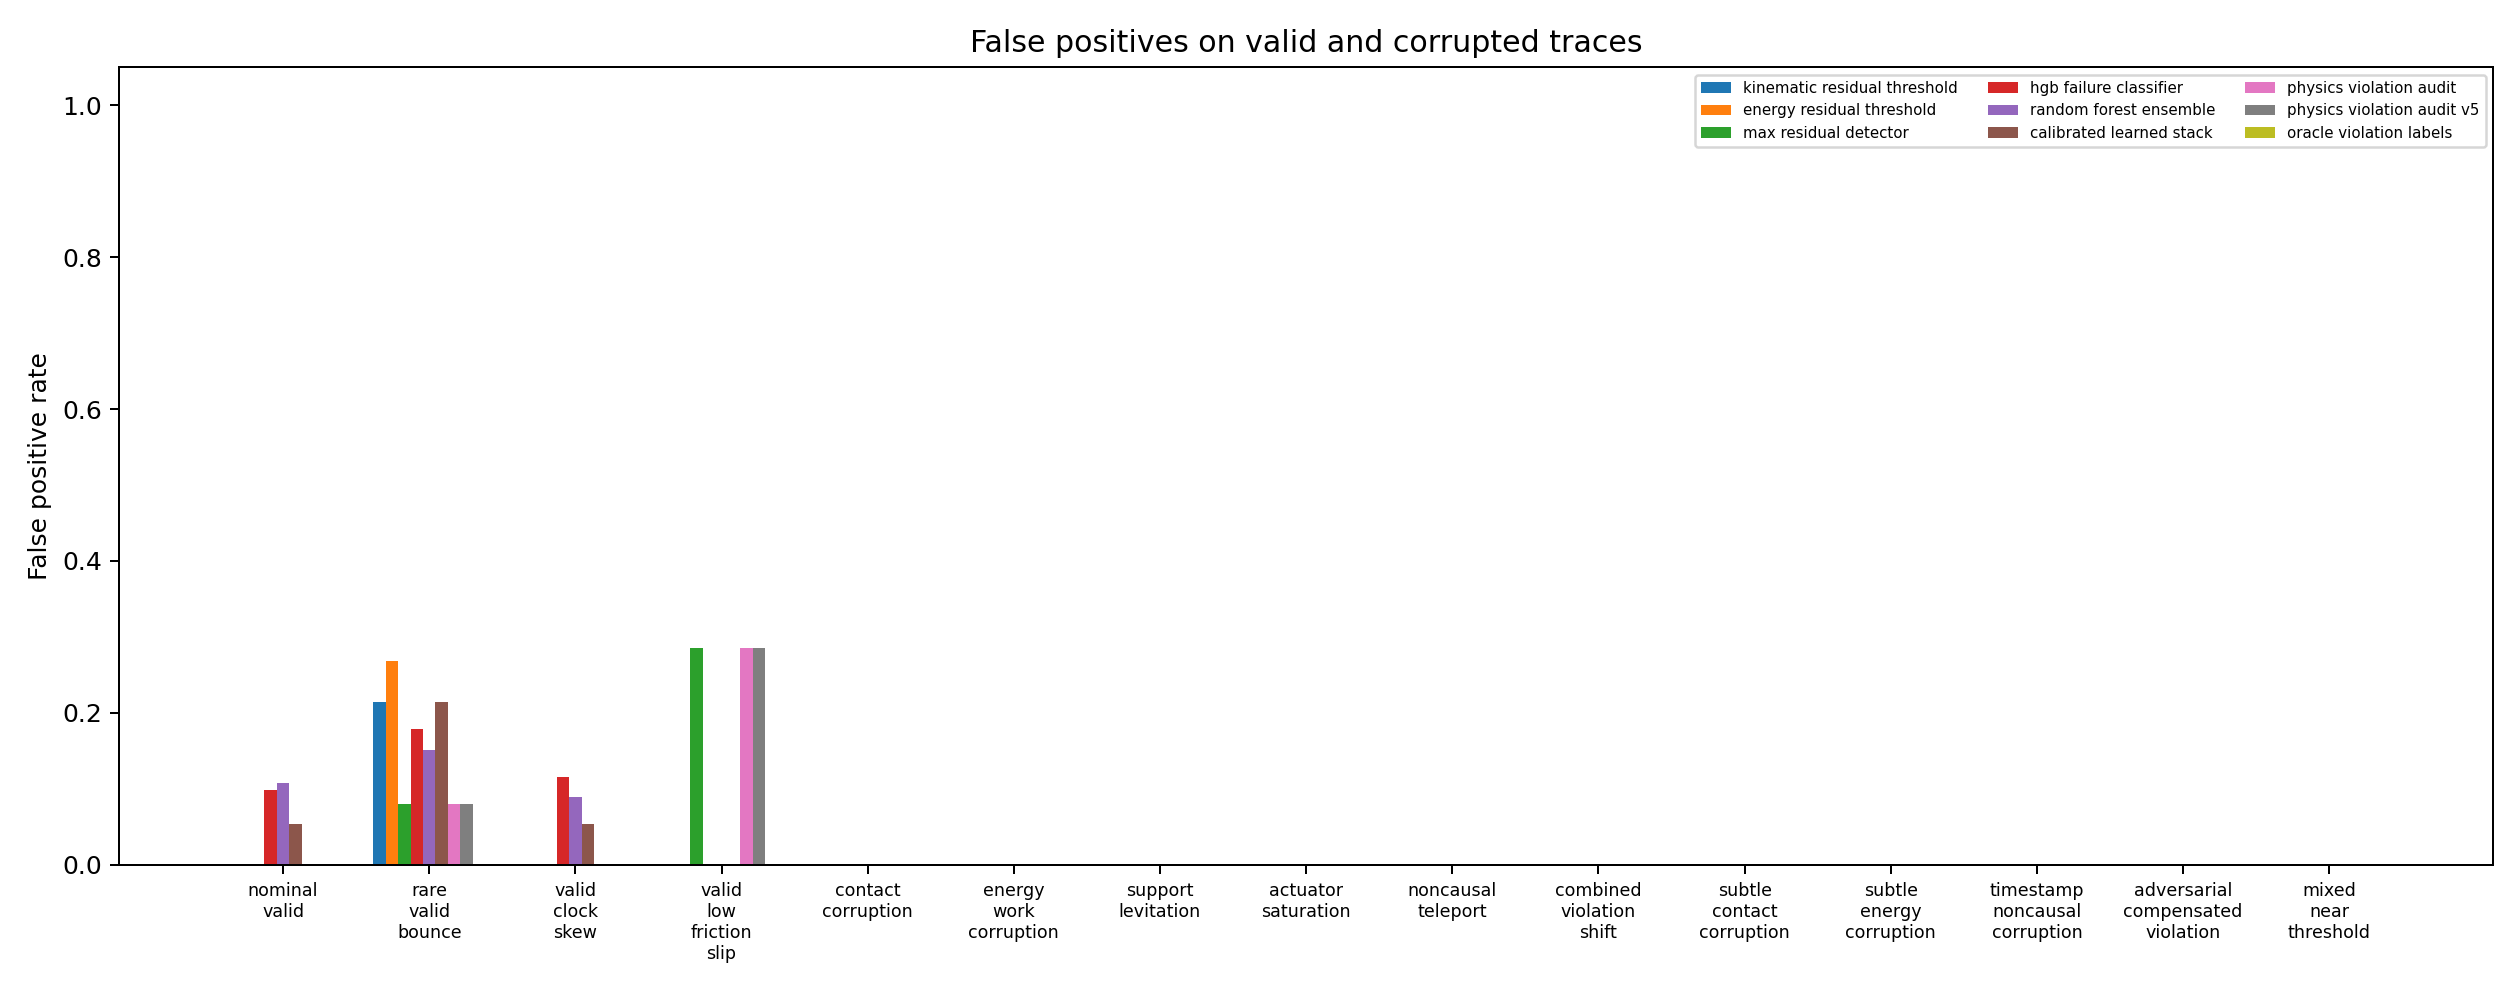
\includegraphics[width=0.92\linewidth]{../figures/physics_audit_false_positive_by_split.png}
\caption{False-positive rates across valid and corrupted splits. Rare valid contact and clock-skew regimes are the practical deployment pressure tests.}
\label{fig:falsepos}
\end{figure}

\section{Fixed-FPR Recall}

\begin{table}[t]
\centering
\caption{Recall at a 5\% false-positive budget. Thresholds are calibrated from valid-regime scores.}
\label{tab:fixed-fpr}
\scriptsize
\begin{tabular}{lrrr}
\toprule
Method & Threshold & Hard recall & Valid scores \\
\midrule
Random & 0.989 & 0.057 & 448 \\
Kin. residual & 2.045 & 0.545 & 448 \\
Energy residual & 3.857 & 0.230 & 448 \\
Contact residual & 0.066 & 0.279 & 448 \\
Max residual & 478.362 & 0.313 & 448 \\
Logistic stack & 0.674 & 0.843 & 448 \\
HGB classifier & 0.027 & 1.000 & 448 \\
RF ensemble & 0.402 & 1.000 & 448 \\
IsolationForest & 0.607 & 0.463 & 448 \\
PCA recon. & 0.019 & 0.944 & 448 \\
Conformal residual & 1.283 & 0.881 & 448 \\
Calibrated stack & 0.046 & 1.000 & 448 \\
Old audit & 299.210 & 0.313 & 448 \\
Audit v5 & 267.118 & 0.308 & 448 \\
Oracle labels & 0.000 & 1.000 & 448 \\
\bottomrule
\end{tabular}
\end{table}


The fixed-FPR analysis prevents a detector from winning merely by flagging everything. Thresholds are calibrated from valid-regime scores, then recall is measured on hard corruptions. Audit v5 trails HGB, random-forest, PCA, conformal, and calibrated-stack baselines at the 5\% false-positive budget. This is a decisive submission blocker.

\section{Ablations}

\begin{table}[t]
\centering
\caption{Combined-shift ablations. A mechanism is not identified if removed components match full v5.}
\label{tab:ablation-combined}
\scriptsize
\begin{tabular}{lrrrr}
\toprule
Variant & Episodes & F1 & Precision & Recall \\
\midrule
Full v5 & 80 & 1.000 & 1.000 & 1.000 \\
No actuator & 80 & 1.000 & 1.000 & 1.000 \\
No causality & 80 & 1.000 & 1.000 & 1.000 \\
No conformal agg. & 80 & 1.000 & 1.000 & 1.000 \\
No contact & 80 & 1.000 & 1.000 & 1.000 \\
No energy & 80 & 1.000 & 1.000 & 1.000 \\
No friction & 80 & 1.000 & 1.000 & 1.000 \\
No rare-valid & 80 & 1.000 & 1.000 & 1.000 \\
No support & 80 & 1.000 & 1.000 & 1.000 \\
No timestamp & 80 & 1.000 & 1.000 & 1.000 \\
Old v4 & 80 & 1.000 & 1.000 & 1.000 \\
Scalar only & 80 & 1.000 & 1.000 & 1.000 \\
\bottomrule
\end{tabular}
\end{table}


The ablation result is not flattering. Several components can be removed without hurting combined-shift F1. The scalar-only variant also matches the full audit on the easy combined split. This does not prove the components are useless in all possible worlds, but it proves the frozen evidence does not identify them as necessary.

\begin{figure}[t]
\centering
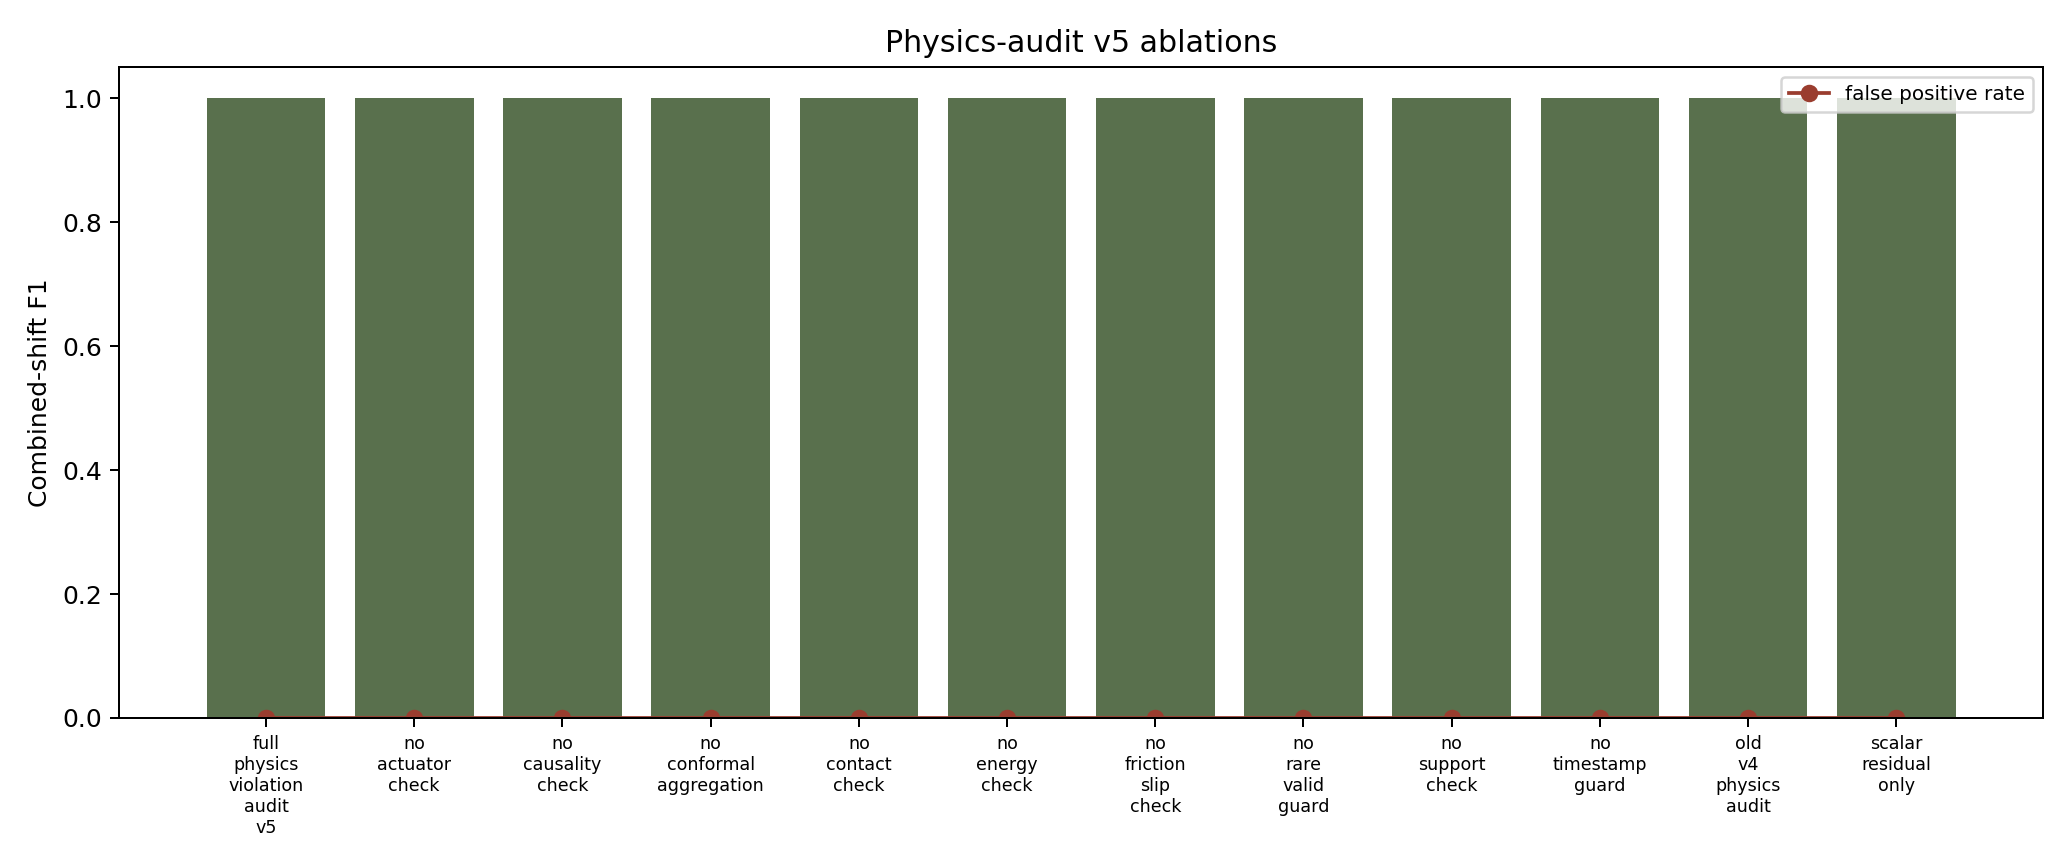
\includegraphics[width=0.86\linewidth]{../figures/physics_audit_ablation_f1.png}
\caption{Combined-shift ablations. The benchmark is too easy for mechanism identification: many variants match full v5.}
\label{fig:ablation}
\end{figure}

\section{Stress Sweep}

\begin{table}[t]
\centering
\caption{Maximum-stress trajectory. Entries are F1 on the combined-violation stress split.}
\label{tab:stress}
\scriptsize
\begin{tabular}{lrrrrrr}
\toprule
Method & 0.00 & 0.20 & 0.40 & 0.60 & 0.80 & 1.00 \\
\midrule
Kin. residual & 1.000 & 1.000 & 1.000 & 1.000 & 1.000 & 1.000 \\
Energy residual & 0.000 & 0.000 & 0.529 & 0.968 & 1.000 & 1.000 \\
Max residual & 0.400 & 0.836 & 1.000 & 1.000 & 1.000 & 1.000 \\
HGB classifier & 1.000 & 1.000 & 1.000 & 1.000 & 1.000 & 1.000 \\
RF ensemble & 1.000 & 1.000 & 1.000 & 1.000 & 1.000 & 1.000 \\
Calibrated stack & 1.000 & 1.000 & 1.000 & 1.000 & 1.000 & 1.000 \\
Audit v5 & 0.420 & 0.815 & 1.000 & 1.000 & 1.000 & 1.000 \\
\bottomrule
\end{tabular}
\end{table}


The stress sweep jointly changes corruption severity, sensor noise, and valid-regime difficulty. The maximum-stress gate is designed to expose methods that work only at a convenient threshold. The frozen decision rule marks the paper killed if v5 loses the maximum-stress gate to any non-oracle baseline.

\begin{figure}[t]
\centering
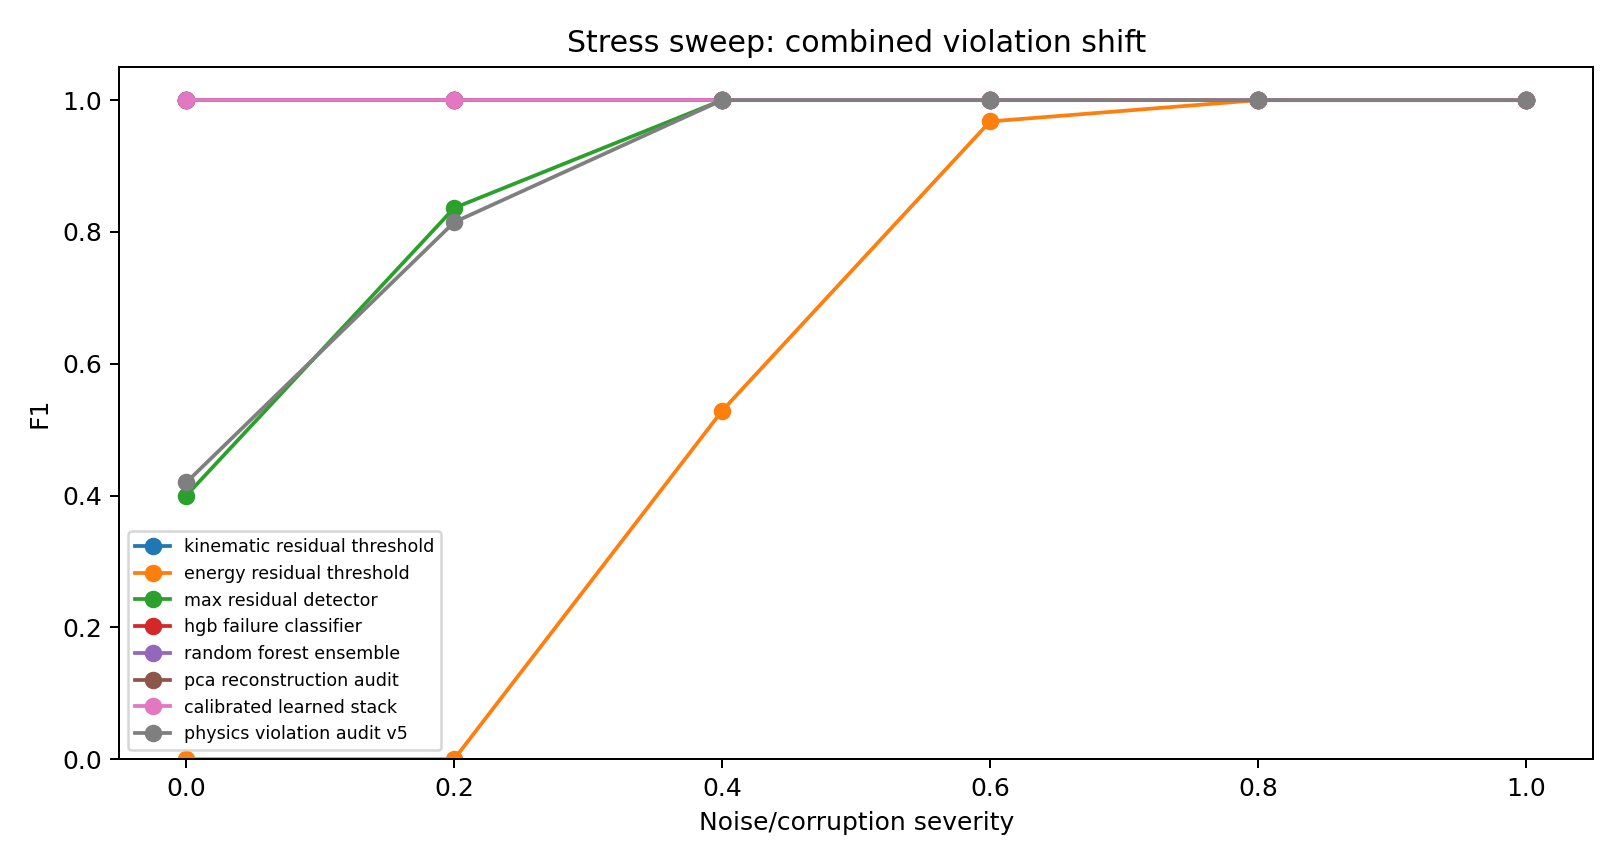
\includegraphics[width=0.86\linewidth]{../figures/physics_audit_stress_sweep.png}
\caption{Stress sweep on the combined-violation split. Strong learned/residual baselines remain competitive or superior.}
\label{fig:stress}
\end{figure}

\section{Interpretation}

The result should be read narrowly and honestly. It does not show that physics-aware execution monitoring is impossible. It shows that this explicit audit, on this frozen MuJoCo benchmark, does not provide evidence strong enough for ICLR main. Three mechanisms undermine the claim.

First, scalar and learned baselines are too strong. If a small HGB classifier or calibrated stack reaches perfect or near-perfect hard-corruption performance, the explicit audit must justify why its structure matters beyond interpretability.

Second, false positives remain a deployment problem. Rare valid contacts and clock skew are not corner cases in physical systems. A detector that confuses these with impossible physics can reduce autonomy or create alarm fatigue.

Third, ablations do not identify the mechanism. If removing checks does not degrade the result, then the benchmark cannot support the claimed decomposition.

\section{Limitations}

This is still a MuJoCo benchmark, not a hardware benchmark. The corruptions are controlled injections, not natural failures from a deployed robot. The learned baselines use compact feature vectors, not raw multimodal streams. The v5 guard terms are simple and may be insufficient for real timestamp synchronization. The oracle is label-only and is not deployable. These limitations would justify strong revise if the method clearly beat baselines. It does not.

\section{Reproducibility}

The final PDF is generated from frozen CSV artifacts. The build script first renders \texttt{paper/generated/*.tex}, then compiles the manuscript, then copies the numbered PDF to \texttt{C:/Users/wangz/Downloads/69.pdf}. No PDF is copied to Desktop. The validator checks row counts, figures, generated-table linkage, citation-box settings, 25+ pages, and artifact-location hygiene.

\section{Decision}

The terminal decision is \textbf{\PaperDecision}. The frozen reason is:

\begin{quote}
\PaperDecisionReason
\end{quote}

The correct action is to archive this as a negative result. A credible revival would need hardware or public benchmark logs, non-injected natural failures, stronger timestamp calibration, impact-aware false-positive controls, and evidence that explicit physics structure beats learned/residual monitors at a fixed false-positive budget.

\begin{table}[t]
\centering
\caption{Pre-specified negative cases beyond the local benchmark scope.}
\label{tab:negative-cases}
\scriptsize
\begin{tabular}{p{0.22\linewidth}p{0.34\linewidth}p{0.34\linewidth}}
\toprule
Case & Observed failure mode & Submission implication \\
\midrule
sensor timestamp skew & causality checks can flag asynchronous but physically valid traces & needs timestamp calibration before deployment claims \\
legal rare bouncing contact & high contact impulse can be physically valid and can trigger contact residuals & requires impact-aware thresholds or learned contact regimes \\
out of distribution deformable object & rigid-body audit assumes object state and contact geometry that may be invalid & scope is rigid-body MuJoCo manipulation \\
semantic task violation with valid physics & all physics checks pass while the robot performs the wrong task & audit is not a complete safety monitor \\
adversarial compensated violation & corruption can be partially hidden by plausible work and contact proxies & scalar residuals and explicit checks both need stronger temporal modeling \\
\bottomrule
\end{tabular}
\end{table}


\clearpage
\appendix

\section{Full Main Metrics}
{\scriptsize
\setlength{\tabcolsep}{2.5pt}
\begin{longtable}{llrrrrrr}
\caption{Full split-level main metrics.}\label{tab:full-metrics}\\
\toprule
Split & Method & Episodes & F1 & Prec. & Rec. & FPR & AUROC \\
\midrule
\endfirsthead
\toprule
Split & Method & Episodes & F1 & Prec. & Rec. & FPR & AUROC \\
\midrule
\endhead
actuator\_saturation & Random & 112 & 0.690 & 1.000 & 0.527 & 0.000 & 0.000 \\
actuator\_saturation & Kin. residual & 112 & 0.000 & 0.000 & 0.000 & 0.000 & 0.000 \\
actuator\_saturation & Energy residual & 112 & 0.000 & 0.000 & 0.000 & 0.000 & 0.000 \\
actuator\_saturation & Contact residual & 112 & 0.018 & 1.000 & 0.009 & 0.000 & 0.000 \\
actuator\_saturation & Max residual & 112 & 0.377 & 1.000 & 0.232 & 0.000 & 0.000 \\
actuator\_saturation & Logistic stack & 112 & 0.880 & 1.000 & 0.786 & 0.000 & 0.000 \\
actuator\_saturation & HGB classifier & 112 & 1.000 & 1.000 & 1.000 & 0.000 & 0.000 \\
actuator\_saturation & RF ensemble & 112 & 1.000 & 1.000 & 1.000 & 0.000 & 0.000 \\
actuator\_saturation & IsolationForest & 112 & 0.000 & 0.000 & 0.000 & 0.000 & 0.000 \\
actuator\_saturation & PCA recon. & 112 & 1.000 & 1.000 & 1.000 & 0.000 & 0.000 \\
actuator\_saturation & Conformal residual & 112 & 0.783 & 1.000 & 0.643 & 0.000 & 0.000 \\
actuator\_saturation & Calibrated stack & 112 & 1.000 & 1.000 & 1.000 & 0.000 & 0.000 \\
actuator\_saturation & Old audit & 112 & 0.377 & 1.000 & 0.232 & 0.000 & 0.000 \\
actuator\_saturation & Audit v5 & 112 & 0.365 & 1.000 & 0.223 & 0.000 & 0.000 \\
actuator\_saturation & Oracle labels & 112 & 1.000 & 1.000 & 1.000 & 0.000 & 0.000 \\
adversarial\_compensated\_violation & Random & 112 & 0.626 & 1.000 & 0.455 & 0.000 & 0.000 \\
adversarial\_compensated\_violation & Kin. residual & 112 & 1.000 & 1.000 & 1.000 & 0.000 & 0.000 \\
adversarial\_compensated\_violation & Energy residual & 112 & 0.486 & 1.000 & 0.321 & 0.000 & 0.000 \\
adversarial\_compensated\_violation & Contact residual & 112 & 1.000 & 1.000 & 1.000 & 0.000 & 0.000 \\
adversarial\_compensated\_violation & Max residual & 112 & 0.742 & 1.000 & 0.589 & 0.000 & 0.000 \\
adversarial\_compensated\_violation & Logistic stack & 112 & 0.991 & 1.000 & 0.982 & 0.000 & 0.000 \\
adversarial\_compensated\_violation & HGB classifier & 112 & 1.000 & 1.000 & 1.000 & 0.000 & 0.000 \\
adversarial\_compensated\_violation & RF ensemble & 112 & 1.000 & 1.000 & 1.000 & 0.000 & 0.000 \\
adversarial\_compensated\_violation & IsolationForest & 112 & 1.000 & 1.000 & 1.000 & 0.000 & 0.000 \\
adversarial\_compensated\_violation & PCA recon. & 112 & 1.000 & 1.000 & 1.000 & 0.000 & 0.000 \\
adversarial\_compensated\_violation & Conformal residual & 112 & 1.000 & 1.000 & 1.000 & 0.000 & 0.000 \\
adversarial\_compensated\_violation & Calibrated stack & 112 & 1.000 & 1.000 & 1.000 & 0.000 & 0.000 \\
adversarial\_compensated\_violation & Old audit & 112 & 0.742 & 1.000 & 0.589 & 0.000 & 0.000 \\
adversarial\_compensated\_violation & Audit v5 & 112 & 0.742 & 1.000 & 0.589 & 0.000 & 0.000 \\
adversarial\_compensated\_violation & Oracle labels & 112 & 1.000 & 1.000 & 1.000 & 0.000 & 0.000 \\
combined\_violation\_shift & Random & 112 & 0.634 & 1.000 & 0.464 & 0.000 & 0.000 \\
combined\_violation\_shift & Kin. residual & 112 & 1.000 & 1.000 & 1.000 & 0.000 & 0.000 \\
combined\_violation\_shift & Energy residual & 112 & 1.000 & 1.000 & 1.000 & 0.000 & 0.000 \\
combined\_violation\_shift & Contact residual & 112 & 0.000 & 0.000 & 0.000 & 0.000 & 0.000 \\
combined\_violation\_shift & Max residual & 112 & 1.000 & 1.000 & 1.000 & 0.000 & 0.000 \\
combined\_violation\_shift & Logistic stack & 112 & 1.000 & 1.000 & 1.000 & 0.000 & 0.000 \\
combined\_violation\_shift & HGB classifier & 112 & 1.000 & 1.000 & 1.000 & 0.000 & 0.000 \\
combined\_violation\_shift & RF ensemble & 112 & 1.000 & 1.000 & 1.000 & 0.000 & 0.000 \\
combined\_violation\_shift & IsolationForest & 112 & 1.000 & 1.000 & 1.000 & 0.000 & 0.000 \\
combined\_violation\_shift & PCA recon. & 112 & 1.000 & 1.000 & 1.000 & 0.000 & 0.000 \\
combined\_violation\_shift & Conformal residual & 112 & 1.000 & 1.000 & 1.000 & 0.000 & 0.000 \\
combined\_violation\_shift & Calibrated stack & 112 & 1.000 & 1.000 & 1.000 & 0.000 & 0.000 \\
combined\_violation\_shift & Old audit & 112 & 1.000 & 1.000 & 1.000 & 0.000 & 0.000 \\
combined\_violation\_shift & Audit v5 & 112 & 1.000 & 1.000 & 1.000 & 0.000 & 0.000 \\
combined\_violation\_shift & Oracle labels & 112 & 1.000 & 1.000 & 1.000 & 0.000 & 0.000 \\
contact\_corruption & Random & 112 & 0.762 & 1.000 & 0.616 & 0.000 & 0.000 \\
contact\_corruption & Kin. residual & 112 & 0.000 & 0.000 & 0.000 & 0.000 & 0.000 \\
contact\_corruption & Energy residual & 112 & 0.000 & 0.000 & 0.000 & 0.000 & 0.000 \\
contact\_corruption & Contact residual & 112 & 1.000 & 1.000 & 1.000 & 0.000 & 0.000 \\
contact\_corruption & Max residual & 112 & 0.000 & 0.000 & 0.000 & 0.000 & 0.000 \\
contact\_corruption & Logistic stack & 112 & 1.000 & 1.000 & 1.000 & 0.000 & 0.000 \\
contact\_corruption & HGB classifier & 112 & 1.000 & 1.000 & 1.000 & 0.000 & 0.000 \\
contact\_corruption & RF ensemble & 112 & 1.000 & 1.000 & 1.000 & 0.000 & 0.000 \\
contact\_corruption & IsolationForest & 112 & 1.000 & 1.000 & 1.000 & 0.000 & 0.000 \\
contact\_corruption & PCA recon. & 112 & 1.000 & 1.000 & 1.000 & 0.000 & 0.000 \\
contact\_corruption & Conformal residual & 112 & 1.000 & 1.000 & 1.000 & 0.000 & 0.000 \\
contact\_corruption & Calibrated stack & 112 & 1.000 & 1.000 & 1.000 & 0.000 & 0.000 \\
contact\_corruption & Old audit & 112 & 0.000 & 0.000 & 0.000 & 0.000 & 0.000 \\
contact\_corruption & Audit v5 & 112 & 0.000 & 0.000 & 0.000 & 0.000 & 0.000 \\
contact\_corruption & Oracle labels & 112 & 1.000 & 1.000 & 1.000 & 0.000 & 0.000 \\
energy\_work\_corruption & Random & 112 & 0.698 & 1.000 & 0.536 & 0.000 & 0.000 \\
energy\_work\_corruption & Kin. residual & 112 & 1.000 & 1.000 & 1.000 & 0.000 & 0.000 \\
energy\_work\_corruption & Energy residual & 112 & 1.000 & 1.000 & 1.000 & 0.000 & 0.000 \\
energy\_work\_corruption & Contact residual & 112 & 0.000 & 0.000 & 0.000 & 0.000 & 0.000 \\
energy\_work\_corruption & Max residual & 112 & 0.365 & 1.000 & 0.223 & 0.000 & 0.000 \\
energy\_work\_corruption & Logistic stack & 112 & 0.938 & 1.000 & 0.884 & 0.000 & 0.000 \\
energy\_work\_corruption & HGB classifier & 112 & 1.000 & 1.000 & 1.000 & 0.000 & 0.000 \\
energy\_work\_corruption & RF ensemble & 112 & 1.000 & 1.000 & 1.000 & 0.000 & 0.000 \\
energy\_work\_corruption & IsolationForest & 112 & 0.316 & 1.000 & 0.188 & 0.000 & 0.000 \\
energy\_work\_corruption & PCA recon. & 112 & 1.000 & 1.000 & 1.000 & 0.000 & 0.000 \\
energy\_work\_corruption & Conformal residual & 112 & 1.000 & 1.000 & 1.000 & 0.000 & 0.000 \\
energy\_work\_corruption & Calibrated stack & 112 & 1.000 & 1.000 & 1.000 & 0.000 & 0.000 \\
energy\_work\_corruption & Old audit & 112 & 0.365 & 1.000 & 0.223 & 0.000 & 0.000 \\
energy\_work\_corruption & Audit v5 & 112 & 0.365 & 1.000 & 0.223 & 0.000 & 0.000 \\
energy\_work\_corruption & Oracle labels & 112 & 1.000 & 1.000 & 1.000 & 0.000 & 0.000 \\
mixed\_near\_threshold & Random & 112 & 0.651 & 1.000 & 0.482 & 0.000 & 0.000 \\
mixed\_near\_threshold & Kin. residual & 112 & 0.953 & 1.000 & 0.911 & 0.000 & 0.000 \\
mixed\_near\_threshold & Energy residual & 112 & 0.018 & 1.000 & 0.009 & 0.000 & 0.000 \\
mixed\_near\_threshold & Contact residual & 112 & 0.000 & 0.000 & 0.000 & 0.000 & 0.000 \\
mixed\_near\_threshold & Max residual & 112 & 0.000 & 0.000 & 0.000 & 0.000 & 0.000 \\
mixed\_near\_threshold & Logistic stack & 112 & 1.000 & 1.000 & 1.000 & 0.000 & 0.000 \\
mixed\_near\_threshold & HGB classifier & 112 & 1.000 & 1.000 & 1.000 & 0.000 & 0.000 \\
mixed\_near\_threshold & RF ensemble & 112 & 1.000 & 1.000 & 1.000 & 0.000 & 0.000 \\
mixed\_near\_threshold & IsolationForest & 112 & 0.086 & 1.000 & 0.045 & 0.000 & 0.000 \\
mixed\_near\_threshold & PCA recon. & 112 & 1.000 & 1.000 & 1.000 & 0.000 & 0.000 \\
mixed\_near\_threshold & Conformal residual & 112 & 0.000 & 0.000 & 0.000 & 0.000 & 0.000 \\
mixed\_near\_threshold & Calibrated stack & 112 & 1.000 & 1.000 & 1.000 & 0.000 & 0.000 \\
mixed\_near\_threshold & Old audit & 112 & 0.000 & 0.000 & 0.000 & 0.000 & 0.000 \\
mixed\_near\_threshold & Audit v5 & 112 & 0.000 & 0.000 & 0.000 & 0.000 & 0.000 \\
mixed\_near\_threshold & Oracle labels & 112 & 1.000 & 1.000 & 1.000 & 0.000 & 0.000 \\
nominal\_valid & Random & 112 & 0.000 & 0.000 & 0.000 & 0.438 & 0.000 \\
nominal\_valid & Kin. residual & 112 & 0.000 & 0.000 & 0.000 & 0.000 & 0.000 \\
nominal\_valid & Energy residual & 112 & 0.000 & 0.000 & 0.000 & 0.000 & 0.000 \\
nominal\_valid & Contact residual & 112 & 0.000 & 0.000 & 0.000 & 0.009 & 0.000 \\
nominal\_valid & Max residual & 112 & 0.000 & 0.000 & 0.000 & 0.000 & 0.000 \\
nominal\_valid & Logistic stack & 112 & 0.000 & 0.000 & 0.000 & 0.000 & 0.000 \\
nominal\_valid & HGB classifier & 112 & 0.000 & 0.000 & 0.000 & 0.098 & 0.000 \\
nominal\_valid & RF ensemble & 112 & 0.000 & 0.000 & 0.000 & 0.107 & 0.000 \\
nominal\_valid & IsolationForest & 112 & 0.000 & 0.000 & 0.000 & 0.000 & 0.000 \\
nominal\_valid & PCA recon. & 112 & 0.000 & 0.000 & 0.000 & 0.054 & 0.000 \\
nominal\_valid & Conformal residual & 112 & 0.000 & 0.000 & 0.000 & 0.000 & 0.000 \\
nominal\_valid & Calibrated stack & 112 & 0.000 & 0.000 & 0.000 & 0.054 & 0.000 \\
nominal\_valid & Old audit & 112 & 0.000 & 0.000 & 0.000 & 0.000 & 0.000 \\
nominal\_valid & Audit v5 & 112 & 0.000 & 0.000 & 0.000 & 0.000 & 0.000 \\
nominal\_valid & Oracle labels & 112 & 0.000 & 0.000 & 0.000 & 0.000 & 0.000 \\
noncausal\_teleport & Random & 112 & 0.675 & 1.000 & 0.509 & 0.000 & 0.000 \\
noncausal\_teleport & Kin. residual & 112 & 1.000 & 1.000 & 1.000 & 0.000 & 0.000 \\
noncausal\_teleport & Energy residual & 112 & 0.000 & 0.000 & 0.000 & 0.000 & 0.000 \\
noncausal\_teleport & Contact residual & 112 & 0.000 & 0.000 & 0.000 & 0.000 & 0.000 \\
noncausal\_teleport & Max residual & 112 & 1.000 & 1.000 & 1.000 & 0.000 & 0.000 \\
noncausal\_teleport & Logistic stack & 112 & 0.996 & 1.000 & 0.991 & 0.000 & 0.000 \\
noncausal\_teleport & HGB classifier & 112 & 1.000 & 1.000 & 1.000 & 0.000 & 0.000 \\
noncausal\_teleport & RF ensemble & 112 & 1.000 & 1.000 & 1.000 & 0.000 & 0.000 \\
noncausal\_teleport & IsolationForest & 112 & 0.000 & 0.000 & 0.000 & 0.000 & 0.000 \\
noncausal\_teleport & PCA recon. & 112 & 1.000 & 1.000 & 1.000 & 0.000 & 0.000 \\
noncausal\_teleport & Conformal residual & 112 & 1.000 & 1.000 & 1.000 & 0.000 & 0.000 \\
noncausal\_teleport & Calibrated stack & 112 & 1.000 & 1.000 & 1.000 & 0.000 & 0.000 \\
noncausal\_teleport & Old audit & 112 & 1.000 & 1.000 & 1.000 & 0.000 & 0.000 \\
noncausal\_teleport & Audit v5 & 112 & 1.000 & 1.000 & 1.000 & 0.000 & 0.000 \\
noncausal\_teleport & Oracle labels & 112 & 1.000 & 1.000 & 1.000 & 0.000 & 0.000 \\
rare\_valid\_bounce & Random & 112 & 0.000 & 0.000 & 0.000 & 0.464 & 0.000 \\
rare\_valid\_bounce & Kin. residual & 112 & 0.000 & 0.000 & 0.000 & 0.214 & 0.000 \\
rare\_valid\_bounce & Energy residual & 112 & 0.000 & 0.000 & 0.000 & 0.268 & 0.000 \\
rare\_valid\_bounce & Contact residual & 112 & 0.000 & 0.000 & 0.000 & 0.143 & 0.000 \\
rare\_valid\_bounce & Max residual & 112 & 0.000 & 0.000 & 0.000 & 0.080 & 0.000 \\
rare\_valid\_bounce & Logistic stack & 112 & 0.000 & 0.000 & 0.000 & 0.205 & 0.000 \\
rare\_valid\_bounce & HGB classifier & 112 & 0.000 & 0.000 & 0.000 & 0.179 & 0.000 \\
rare\_valid\_bounce & RF ensemble & 112 & 0.000 & 0.000 & 0.000 & 0.152 & 0.000 \\
rare\_valid\_bounce & IsolationForest & 112 & 0.000 & 0.000 & 0.000 & 0.134 & 0.000 \\
rare\_valid\_bounce & PCA recon. & 112 & 0.000 & 0.000 & 0.000 & 0.330 & 0.000 \\
rare\_valid\_bounce & Conformal residual & 112 & 0.000 & 0.000 & 0.000 & 0.125 & 0.000 \\
rare\_valid\_bounce & Calibrated stack & 112 & 0.000 & 0.000 & 0.000 & 0.214 & 0.000 \\
rare\_valid\_bounce & Old audit & 112 & 0.000 & 0.000 & 0.000 & 0.080 & 0.000 \\
rare\_valid\_bounce & Audit v5 & 112 & 0.000 & 0.000 & 0.000 & 0.080 & 0.000 \\
rare\_valid\_bounce & Oracle labels & 112 & 0.000 & 0.000 & 0.000 & 0.000 & 0.000 \\
subtle\_contact\_corruption & Random & 112 & 0.735 & 1.000 & 0.580 & 0.000 & 0.000 \\
subtle\_contact\_corruption & Kin. residual & 112 & 0.000 & 0.000 & 0.000 & 0.000 & 0.000 \\
subtle\_contact\_corruption & Energy residual & 112 & 0.000 & 0.000 & 0.000 & 0.000 & 0.000 \\
subtle\_contact\_corruption & Contact residual & 112 & 1.000 & 1.000 & 1.000 & 0.000 & 0.000 \\
subtle\_contact\_corruption & Max residual & 112 & 0.000 & 0.000 & 0.000 & 0.000 & 0.000 \\
subtle\_contact\_corruption & Logistic stack & 112 & 0.953 & 1.000 & 0.911 & 0.000 & 0.000 \\
subtle\_contact\_corruption & HGB classifier & 112 & 1.000 & 1.000 & 1.000 & 0.000 & 0.000 \\
subtle\_contact\_corruption & RF ensemble & 112 & 1.000 & 1.000 & 1.000 & 0.000 & 0.000 \\
subtle\_contact\_corruption & IsolationForest & 112 & 1.000 & 1.000 & 1.000 & 0.000 & 0.000 \\
subtle\_contact\_corruption & PCA recon. & 112 & 1.000 & 1.000 & 1.000 & 0.000 & 0.000 \\
subtle\_contact\_corruption & Conformal residual & 112 & 1.000 & 1.000 & 1.000 & 0.000 & 0.000 \\
subtle\_contact\_corruption & Calibrated stack & 112 & 1.000 & 1.000 & 1.000 & 0.000 & 0.000 \\
subtle\_contact\_corruption & Old audit & 112 & 0.000 & 0.000 & 0.000 & 0.000 & 0.000 \\
subtle\_contact\_corruption & Audit v5 & 112 & 0.000 & 0.000 & 0.000 & 0.000 & 0.000 \\
subtle\_contact\_corruption & Oracle labels & 112 & 1.000 & 1.000 & 1.000 & 0.000 & 0.000 \\
subtle\_energy\_corruption & Random & 112 & 0.735 & 1.000 & 0.580 & 0.000 & 0.000 \\
subtle\_energy\_corruption & Kin. residual & 112 & 0.000 & 0.000 & 0.000 & 0.000 & 0.000 \\
subtle\_energy\_corruption & Energy residual & 112 & 0.000 & 0.000 & 0.000 & 0.000 & 0.000 \\
subtle\_energy\_corruption & Contact residual & 112 & 0.035 & 1.000 & 0.018 & 0.000 & 0.000 \\
subtle\_energy\_corruption & Max residual & 112 & 0.000 & 0.000 & 0.000 & 0.000 & 0.000 \\
subtle\_energy\_corruption & Logistic stack & 112 & 0.018 & 1.000 & 0.009 & 0.000 & 0.000 \\
subtle\_energy\_corruption & HGB classifier & 112 & 1.000 & 1.000 & 1.000 & 0.000 & 0.000 \\
subtle\_energy\_corruption & RF ensemble & 112 & 1.000 & 1.000 & 1.000 & 0.000 & 0.000 \\
subtle\_energy\_corruption & IsolationForest & 112 & 0.000 & 0.000 & 0.000 & 0.000 & 0.000 \\
subtle\_energy\_corruption & PCA recon. & 112 & 0.808 & 1.000 & 0.679 & 0.000 & 0.000 \\
subtle\_energy\_corruption & Conformal residual & 112 & 0.000 & 0.000 & 0.000 & 0.000 & 0.000 \\
subtle\_energy\_corruption & Calibrated stack & 112 & 1.000 & 1.000 & 1.000 & 0.000 & 0.000 \\
subtle\_energy\_corruption & Old audit & 112 & 0.000 & 0.000 & 0.000 & 0.000 & 0.000 \\
subtle\_energy\_corruption & Audit v5 & 112 & 0.000 & 0.000 & 0.000 & 0.000 & 0.000 \\
subtle\_energy\_corruption & Oracle labels & 112 & 1.000 & 1.000 & 1.000 & 0.000 & 0.000 \\
support\_levitation & Random & 112 & 0.690 & 1.000 & 0.527 & 0.000 & 0.000 \\
support\_levitation & Kin. residual & 112 & 1.000 & 1.000 & 1.000 & 0.000 & 0.000 \\
support\_levitation & Energy residual & 112 & 0.507 & 1.000 & 0.339 & 0.000 & 0.000 \\
support\_levitation & Contact residual & 112 & 0.000 & 0.000 & 0.000 & 0.000 & 0.000 \\
support\_levitation & Max residual & 112 & 0.000 & 0.000 & 0.000 & 0.000 & 0.000 \\
support\_levitation & Logistic stack & 112 & 1.000 & 1.000 & 1.000 & 0.000 & 0.000 \\
support\_levitation & HGB classifier & 112 & 1.000 & 1.000 & 1.000 & 0.000 & 0.000 \\
support\_levitation & RF ensemble & 112 & 1.000 & 1.000 & 1.000 & 0.000 & 0.000 \\
support\_levitation & IsolationForest & 112 & 0.018 & 1.000 & 0.009 & 0.000 & 0.000 \\
support\_levitation & PCA recon. & 112 & 1.000 & 1.000 & 1.000 & 0.000 & 0.000 \\
support\_levitation & Conformal residual & 112 & 1.000 & 1.000 & 1.000 & 0.000 & 0.000 \\
support\_levitation & Calibrated stack & 112 & 1.000 & 1.000 & 1.000 & 0.000 & 0.000 \\
support\_levitation & Old audit & 112 & 0.000 & 0.000 & 0.000 & 0.000 & 0.000 \\
support\_levitation & Audit v5 & 112 & 0.000 & 0.000 & 0.000 & 0.000 & 0.000 \\
support\_levitation & Oracle labels & 112 & 1.000 & 1.000 & 1.000 & 0.000 & 0.000 \\
timestamp\_noncausal\_corruption & Random & 112 & 0.705 & 1.000 & 0.545 & 0.000 & 0.000 \\
timestamp\_noncausal\_corruption & Kin. residual & 112 & 0.179 & 1.000 & 0.098 & 0.000 & 0.000 \\
timestamp\_noncausal\_corruption & Energy residual & 112 & 0.000 & 0.000 & 0.000 & 0.000 & 0.000 \\
timestamp\_noncausal\_corruption & Contact residual & 112 & 0.000 & 0.000 & 0.000 & 0.000 & 0.000 \\
timestamp\_noncausal\_corruption & Max residual & 112 & 0.698 & 1.000 & 0.536 & 0.000 & 0.000 \\
timestamp\_noncausal\_corruption & Logistic stack & 112 & 0.815 & 1.000 & 0.688 & 0.000 & 0.000 \\
timestamp\_noncausal\_corruption & HGB classifier & 112 & 1.000 & 1.000 & 1.000 & 0.000 & 0.000 \\
timestamp\_noncausal\_corruption & RF ensemble & 112 & 1.000 & 1.000 & 1.000 & 0.000 & 0.000 \\
timestamp\_noncausal\_corruption & IsolationForest & 112 & 0.000 & 0.000 & 0.000 & 0.000 & 0.000 \\
timestamp\_noncausal\_corruption & PCA recon. & 112 & 1.000 & 1.000 & 1.000 & 0.000 & 0.000 \\
timestamp\_noncausal\_corruption & Conformal residual & 112 & 0.617 & 1.000 & 0.446 & 0.000 & 0.000 \\
timestamp\_noncausal\_corruption & Calibrated stack & 112 & 1.000 & 1.000 & 1.000 & 0.000 & 0.000 \\
timestamp\_noncausal\_corruption & Old audit & 112 & 0.698 & 1.000 & 0.536 & 0.000 & 0.000 \\
timestamp\_noncausal\_corruption & Audit v5 & 112 & 0.690 & 1.000 & 0.527 & 0.000 & 0.000 \\
timestamp\_noncausal\_corruption & Oracle labels & 112 & 1.000 & 1.000 & 1.000 & 0.000 & 0.000 \\
valid\_clock\_skew & Random & 112 & 0.000 & 0.000 & 0.000 & 0.464 & 0.000 \\
valid\_clock\_skew & Kin. residual & 112 & 0.000 & 0.000 & 0.000 & 0.000 & 0.000 \\
valid\_clock\_skew & Energy residual & 112 & 0.000 & 0.000 & 0.000 & 0.000 & 0.000 \\
valid\_clock\_skew & Contact residual & 112 & 0.000 & 0.000 & 0.000 & 0.000 & 0.000 \\
valid\_clock\_skew & Max residual & 112 & 0.000 & 0.000 & 0.000 & 0.000 & 0.000 \\
valid\_clock\_skew & Logistic stack & 112 & 0.000 & 0.000 & 0.000 & 0.000 & 0.000 \\
valid\_clock\_skew & HGB classifier & 112 & 0.000 & 0.000 & 0.000 & 0.116 & 0.000 \\
valid\_clock\_skew & RF ensemble & 112 & 0.000 & 0.000 & 0.000 & 0.089 & 0.000 \\
valid\_clock\_skew & IsolationForest & 112 & 0.000 & 0.000 & 0.000 & 0.000 & 0.000 \\
valid\_clock\_skew & PCA recon. & 112 & 0.000 & 0.000 & 0.000 & 0.054 & 0.000 \\
valid\_clock\_skew & Conformal residual & 112 & 0.000 & 0.000 & 0.000 & 0.000 & 0.000 \\
valid\_clock\_skew & Calibrated stack & 112 & 0.000 & 0.000 & 0.000 & 0.054 & 0.000 \\
valid\_clock\_skew & Old audit & 112 & 0.000 & 0.000 & 0.000 & 0.000 & 0.000 \\
valid\_clock\_skew & Audit v5 & 112 & 0.000 & 0.000 & 0.000 & 0.000 & 0.000 \\
valid\_clock\_skew & Oracle labels & 112 & 0.000 & 0.000 & 0.000 & 0.000 & 0.000 \\
valid\_low\_friction\_slip & Random & 112 & 0.000 & 0.000 & 0.000 & 0.527 & 0.000 \\
valid\_low\_friction\_slip & Kin. residual & 112 & 0.000 & 0.000 & 0.000 & 0.000 & 0.000 \\
valid\_low\_friction\_slip & Energy residual & 112 & 0.000 & 0.000 & 0.000 & 0.000 & 0.000 \\
valid\_low\_friction\_slip & Contact residual & 112 & 0.000 & 0.000 & 0.000 & 0.000 & 0.000 \\
valid\_low\_friction\_slip & Max residual & 112 & 0.000 & 0.000 & 0.000 & 0.286 & 0.000 \\
valid\_low\_friction\_slip & Logistic stack & 112 & 0.000 & 0.000 & 0.000 & 0.000 & 0.000 \\
valid\_low\_friction\_slip & HGB classifier & 112 & 0.000 & 0.000 & 0.000 & 0.000 & 0.000 \\
valid\_low\_friction\_slip & RF ensemble & 112 & 0.000 & 0.000 & 0.000 & 0.000 & 0.000 \\
valid\_low\_friction\_slip & IsolationForest & 112 & 0.000 & 0.000 & 0.000 & 0.000 & 0.000 \\
valid\_low\_friction\_slip & PCA recon. & 112 & 0.000 & 0.000 & 0.000 & 0.000 & 0.000 \\
valid\_low\_friction\_slip & Conformal residual & 112 & 0.000 & 0.000 & 0.000 & 0.009 & 0.000 \\
valid\_low\_friction\_slip & Calibrated stack & 112 & 0.000 & 0.000 & 0.000 & 0.000 & 0.000 \\
valid\_low\_friction\_slip & Old audit & 112 & 0.000 & 0.000 & 0.000 & 0.286 & 0.000 \\
valid\_low\_friction\_slip & Audit v5 & 112 & 0.000 & 0.000 & 0.000 & 0.286 & 0.000 \\
valid\_low\_friction\_slip & Oracle labels & 112 & 0.000 & 0.000 & 0.000 & 0.000 & 0.000 \\
\bottomrule
\end{longtable}
}


\section{Full Aggregate Metrics}
{\scriptsize
\setlength{\tabcolsep}{2.5pt}
\begin{longtable}{llrrrrrr}
\caption{Full aggregate metrics.}\label{tab:full-aggregate}\\
\toprule
Split & Method & Episodes & F1 & Prec. & Rec. & FPR & AUROC \\
\midrule
\endfirsthead
\toprule
Split & Method & Episodes & F1 & Prec. & Rec. & FPR & AUROC \\
\midrule
\endhead
all & Random & 1680 & 0.622 & 0.755 & 0.529 & 0.473 & 0.529 \\
all & Random & 448 & 0.000 & 0.000 & 0.000 & 0.473 & 0.000 \\
all & Random & 1232 & 0.692 & 1.000 & 0.529 & 0.000 & 0.000 \\
all & Random & 336 & 0.637 & 1.000 & 0.467 & 0.000 & 0.000 \\
all & Kin. residual & 1680 & 0.698 & 0.966 & 0.546 & 0.054 & 0.803 \\
all & Kin. residual & 448 & 0.000 & 0.000 & 0.000 & 0.054 & 0.000 \\
all & Kin. residual & 1232 & 0.707 & 1.000 & 0.546 & 0.000 & 0.000 \\
all & Kin. residual & 336 & 0.985 & 1.000 & 0.970 & 0.000 & 0.000 \\
all & Energy residual & 1680 & 0.383 & 0.909 & 0.243 & 0.067 & 0.582 \\
all & Energy residual & 448 & 0.000 & 0.000 & 0.000 & 0.067 & 0.000 \\
all & Energy residual & 1232 & 0.391 & 1.000 & 0.243 & 0.000 & 0.000 \\
all & Energy residual & 336 & 0.614 & 1.000 & 0.444 & 0.000 & 0.000 \\
all & Contact residual & 1680 & 0.427 & 0.952 & 0.275 & 0.038 & 0.609 \\
all & Contact residual & 448 & 0.000 & 0.000 & 0.000 & 0.038 & 0.000 \\
all & Contact residual & 1232 & 0.432 & 1.000 & 0.275 & 0.000 & 0.000 \\
all & Contact residual & 336 & 0.500 & 1.000 & 0.333 & 0.000 & 0.000 \\
all & Max residual & 1680 & 0.479 & 0.907 & 0.326 & 0.091 & 0.470 \\
all & Max residual & 448 & 0.000 & 0.000 & 0.000 & 0.091 & 0.000 \\
all & Max residual & 1232 & 0.491 & 1.000 & 0.326 & 0.000 & 0.000 \\
all & Max residual & 336 & 0.693 & 1.000 & 0.530 & 0.000 & 0.000 \\
all & Logistic stack & 1680 & 0.904 & 0.978 & 0.841 & 0.051 & 0.973 \\
all & Logistic stack & 448 & 0.000 & 0.000 & 0.000 & 0.051 & 0.000 \\
all & Logistic stack & 1232 & 0.914 & 1.000 & 0.841 & 0.000 & 0.000 \\
all & Logistic stack & 336 & 0.997 & 1.000 & 0.994 & 0.000 & 0.000 \\
all & HGB classifier & 1680 & 0.983 & 0.966 & 1.000 & 0.098 & 1.000 \\
all & HGB classifier & 448 & 0.000 & 0.000 & 0.000 & 0.098 & 0.000 \\
all & HGB classifier & 1232 & 1.000 & 1.000 & 1.000 & 0.000 & 0.000 \\
all & HGB classifier & 336 & 1.000 & 1.000 & 1.000 & 0.000 & 0.000 \\
all & RF ensemble & 1680 & 0.984 & 0.969 & 1.000 & 0.087 & 1.000 \\
all & RF ensemble & 448 & 0.000 & 0.000 & 0.000 & 0.087 & 0.000 \\
all & RF ensemble & 1232 & 1.000 & 1.000 & 1.000 & 0.000 & 0.000 \\
all & RF ensemble & 336 & 1.000 & 1.000 & 1.000 & 0.000 & 0.000 \\
all & IsolationForest & 1680 & 0.552 & 0.969 & 0.386 & 0.034 & 0.937 \\
all & IsolationForest & 448 & 0.000 & 0.000 & 0.000 & 0.034 & 0.000 \\
all & IsolationForest & 1232 & 0.556 & 1.000 & 0.386 & 0.000 & 0.000 \\
all & IsolationForest & 336 & 0.811 & 1.000 & 0.681 & 0.000 & 0.000 \\
all & PCA recon. & 1680 & 0.966 & 0.961 & 0.971 & 0.109 & 0.989 \\
all & PCA recon. & 448 & 0.000 & 0.000 & 0.000 & 0.109 & 0.000 \\
all & PCA recon. & 1232 & 0.985 & 1.000 & 0.971 & 0.000 & 0.000 \\
all & PCA recon. & 336 & 1.000 & 1.000 & 1.000 & 0.000 & 0.000 \\
all & Conformal residual & 1680 & 0.842 & 0.984 & 0.735 & 0.034 & 0.947 \\
all & Conformal residual & 448 & 0.000 & 0.000 & 0.000 & 0.034 & 0.000 \\
all & Conformal residual & 1232 & 0.848 & 1.000 & 0.735 & 0.000 & 0.000 \\
all & Conformal residual & 336 & 0.800 & 1.000 & 0.667 & 0.000 & 0.000 \\
all & Calibrated stack & 1680 & 0.986 & 0.972 & 1.000 & 0.080 & 1.000 \\
all & Calibrated stack & 448 & 0.000 & 0.000 & 0.000 & 0.080 & 0.000 \\
all & Calibrated stack & 1232 & 1.000 & 1.000 & 1.000 & 0.000 & 0.000 \\
all & Calibrated stack & 336 & 1.000 & 1.000 & 1.000 & 0.000 & 0.000 \\
all & Old audit & 1680 & 0.479 & 0.907 & 0.326 & 0.091 & 0.471 \\
all & Old audit & 448 & 0.000 & 0.000 & 0.000 & 0.091 & 0.000 \\
all & Old audit & 1232 & 0.491 & 1.000 & 0.326 & 0.000 & 0.000 \\
all & Old audit & 336 & 0.693 & 1.000 & 0.530 & 0.000 & 0.000 \\
all & Audit v5 & 1680 & 0.477 & 0.907 & 0.324 & 0.091 & 0.475 \\
all & Audit v5 & 448 & 0.000 & 0.000 & 0.000 & 0.091 & 0.000 \\
all & Audit v5 & 1232 & 0.489 & 1.000 & 0.324 & 0.000 & 0.000 \\
all & Audit v5 & 336 & 0.693 & 1.000 & 0.530 & 0.000 & 0.000 \\
all & Oracle labels & 1680 & 1.000 & 1.000 & 1.000 & 0.000 & 1.000 \\
all & Oracle labels & 448 & 0.000 & 0.000 & 0.000 & 0.000 & 0.000 \\
all & Oracle labels & 1232 & 1.000 & 1.000 & 1.000 & 0.000 & 0.000 \\
all & Oracle labels & 336 & 1.000 & 1.000 & 1.000 & 0.000 & 0.000 \\
\bottomrule
\end{longtable}
}


\section{Full Ablation Metrics}
{\scriptsize
\setlength{\tabcolsep}{2.5pt}
\begin{longtable}{llrrrrrr}
\caption{Full ablation metrics.}\label{tab:full-ablation}\\
\toprule
Split & Method & Episodes & F1 & Prec. & Rec. & FPR & AUROC \\
\midrule
\endfirsthead
\toprule
Split & Method & Episodes & F1 & Prec. & Rec. & FPR & AUROC \\
\midrule
\endhead
adversarial\_compensated\_violation & Full v5 & 80 & 0.740 & 1.000 & 0.588 & 0.000 & 0.000 \\
adversarial\_compensated\_violation & No actuator & 80 & 0.740 & 1.000 & 0.588 & 0.000 & 0.000 \\
adversarial\_compensated\_violation & No causality & 80 & 0.740 & 1.000 & 0.588 & 0.000 & 0.000 \\
adversarial\_compensated\_violation & No conformal agg. & 80 & 0.740 & 1.000 & 0.588 & 0.000 & 0.000 \\
adversarial\_compensated\_violation & No contact & 80 & 0.740 & 1.000 & 0.588 & 0.000 & 0.000 \\
adversarial\_compensated\_violation & No energy & 80 & 0.740 & 1.000 & 0.588 & 0.000 & 0.000 \\
adversarial\_compensated\_violation & No friction & 80 & 0.797 & 1.000 & 0.662 & 0.000 & 0.000 \\
adversarial\_compensated\_violation & No rare-valid & 80 & 0.740 & 1.000 & 0.588 & 0.000 & 0.000 \\
adversarial\_compensated\_violation & No support & 80 & 0.740 & 1.000 & 0.588 & 0.000 & 0.000 \\
adversarial\_compensated\_violation & No timestamp & 80 & 0.740 & 1.000 & 0.588 & 0.000 & 0.000 \\
adversarial\_compensated\_violation & Old v4 & 80 & 0.740 & 1.000 & 0.588 & 0.000 & 0.000 \\
adversarial\_compensated\_violation & Scalar only & 80 & 0.161 & 1.000 & 0.087 & 0.000 & 0.000 \\
combined\_violation\_shift & Full v5 & 80 & 1.000 & 1.000 & 1.000 & 0.000 & 0.000 \\
combined\_violation\_shift & No actuator & 80 & 1.000 & 1.000 & 1.000 & 0.000 & 0.000 \\
combined\_violation\_shift & No causality & 80 & 1.000 & 1.000 & 1.000 & 0.000 & 0.000 \\
combined\_violation\_shift & No conformal agg. & 80 & 1.000 & 1.000 & 1.000 & 0.000 & 0.000 \\
combined\_violation\_shift & No contact & 80 & 1.000 & 1.000 & 1.000 & 0.000 & 0.000 \\
combined\_violation\_shift & No energy & 80 & 1.000 & 1.000 & 1.000 & 0.000 & 0.000 \\
combined\_violation\_shift & No friction & 80 & 1.000 & 1.000 & 1.000 & 0.000 & 0.000 \\
combined\_violation\_shift & No rare-valid & 80 & 1.000 & 1.000 & 1.000 & 0.000 & 0.000 \\
combined\_violation\_shift & No support & 80 & 1.000 & 1.000 & 1.000 & 0.000 & 0.000 \\
combined\_violation\_shift & No timestamp & 80 & 1.000 & 1.000 & 1.000 & 0.000 & 0.000 \\
combined\_violation\_shift & Old v4 & 80 & 1.000 & 1.000 & 1.000 & 0.000 & 0.000 \\
combined\_violation\_shift & Scalar only & 80 & 1.000 & 1.000 & 1.000 & 0.000 & 0.000 \\
mixed\_near\_threshold & Full v5 & 80 & 0.000 & 0.000 & 0.000 & 0.000 & 0.000 \\
mixed\_near\_threshold & No actuator & 80 & 0.000 & 0.000 & 0.000 & 0.000 & 0.000 \\
mixed\_near\_threshold & No causality & 80 & 0.000 & 0.000 & 0.000 & 0.000 & 0.000 \\
mixed\_near\_threshold & No conformal agg. & 80 & 0.000 & 0.000 & 0.000 & 0.000 & 0.000 \\
mixed\_near\_threshold & No contact & 80 & 0.000 & 0.000 & 0.000 & 0.000 & 0.000 \\
mixed\_near\_threshold & No energy & 80 & 0.000 & 0.000 & 0.000 & 0.000 & 0.000 \\
mixed\_near\_threshold & No friction & 80 & 0.000 & 0.000 & 0.000 & 0.000 & 0.000 \\
mixed\_near\_threshold & No rare-valid & 80 & 0.000 & 0.000 & 0.000 & 0.000 & 0.000 \\
mixed\_near\_threshold & No support & 80 & 0.000 & 0.000 & 0.000 & 0.000 & 0.000 \\
mixed\_near\_threshold & No timestamp & 80 & 0.000 & 0.000 & 0.000 & 0.000 & 0.000 \\
mixed\_near\_threshold & Old v4 & 80 & 0.000 & 0.000 & 0.000 & 0.000 & 0.000 \\
mixed\_near\_threshold & Scalar only & 80 & 0.000 & 0.000 & 0.000 & 0.000 & 0.000 \\
rare\_valid\_bounce & Full v5 & 80 & 0.000 & 0.000 & 0.000 & 0.050 & 0.000 \\
rare\_valid\_bounce & No actuator & 80 & 0.000 & 0.000 & 0.000 & 0.050 & 0.000 \\
rare\_valid\_bounce & No causality & 80 & 0.000 & 0.000 & 0.000 & 0.050 & 0.000 \\
rare\_valid\_bounce & No conformal agg. & 80 & 0.000 & 0.000 & 0.000 & 0.050 & 0.000 \\
rare\_valid\_bounce & No contact & 80 & 0.000 & 0.000 & 0.000 & 0.050 & 0.000 \\
rare\_valid\_bounce & No energy & 80 & 0.000 & 0.000 & 0.000 & 0.050 & 0.000 \\
rare\_valid\_bounce & No friction & 80 & 0.000 & 0.000 & 0.000 & 0.050 & 0.000 \\
rare\_valid\_bounce & No rare-valid & 80 & 0.000 & 0.000 & 0.000 & 0.050 & 0.000 \\
rare\_valid\_bounce & No support & 80 & 0.000 & 0.000 & 0.000 & 0.050 & 0.000 \\
rare\_valid\_bounce & No timestamp & 80 & 0.000 & 0.000 & 0.000 & 0.050 & 0.000 \\
rare\_valid\_bounce & Old v4 & 80 & 0.000 & 0.000 & 0.000 & 0.050 & 0.000 \\
rare\_valid\_bounce & Scalar only & 80 & 0.000 & 0.000 & 0.000 & 0.050 & 0.000 \\
\bottomrule
\end{longtable}
}


\section{Full Stress Metrics}
{\scriptsize
\setlength{\tabcolsep}{2.5pt}
\begin{longtable}{llrrrrrr}
\caption{Full stress-sweep metrics.}\label{tab:full-stress}\\
\toprule
Split & Method & Episodes & F1 & Prec. & Rec. & FPR & AUROC \\
\midrule
\endfirsthead
\toprule
Split & Method & Episodes & F1 & Prec. & Rec. & FPR & AUROC \\
\midrule
\endhead
stress\_0.00\_adversarial\_compensated\_violation & Kin. residual & 64 & 0.476 & 1.000 & 0.312 & 0.000 & 0.000 \\
stress\_0.00\_adversarial\_compensated\_violation & Energy residual & 64 & 0.562 & 1.000 & 0.391 & 0.000 & 0.000 \\
stress\_0.00\_adversarial\_compensated\_violation & Max residual & 64 & 0.000 & 0.000 & 0.000 & 0.000 & 0.000 \\
stress\_0.00\_adversarial\_compensated\_violation & HGB classifier & 64 & 1.000 & 1.000 & 1.000 & 0.000 & 0.000 \\
stress\_0.00\_adversarial\_compensated\_violation & RF ensemble & 64 & 1.000 & 1.000 & 1.000 & 0.000 & 0.000 \\
stress\_0.00\_adversarial\_compensated\_violation & PCA recon. & 64 & 0.897 & 1.000 & 0.812 & 0.000 & 0.000 \\
stress\_0.00\_adversarial\_compensated\_violation & Calibrated stack & 64 & 1.000 & 1.000 & 1.000 & 0.000 & 0.000 \\
stress\_0.00\_adversarial\_compensated\_violation & Audit v5 & 64 & 0.000 & 0.000 & 0.000 & 0.000 & 0.000 \\
stress\_0.00\_combined\_violation\_shift & Kin. residual & 64 & 1.000 & 1.000 & 1.000 & 0.000 & 0.000 \\
stress\_0.00\_combined\_violation\_shift & Energy residual & 64 & 0.000 & 0.000 & 0.000 & 0.000 & 0.000 \\
stress\_0.00\_combined\_violation\_shift & Max residual & 64 & 0.400 & 1.000 & 0.250 & 0.000 & 0.000 \\
stress\_0.00\_combined\_violation\_shift & HGB classifier & 64 & 1.000 & 1.000 & 1.000 & 0.000 & 0.000 \\
stress\_0.00\_combined\_violation\_shift & RF ensemble & 64 & 1.000 & 1.000 & 1.000 & 0.000 & 0.000 \\
stress\_0.00\_combined\_violation\_shift & PCA recon. & 64 & 1.000 & 1.000 & 1.000 & 0.000 & 0.000 \\
stress\_0.00\_combined\_violation\_shift & Calibrated stack & 64 & 1.000 & 1.000 & 1.000 & 0.000 & 0.000 \\
stress\_0.00\_combined\_violation\_shift & Audit v5 & 64 & 0.420 & 1.000 & 0.266 & 0.000 & 0.000 \\
stress\_0.00\_rare\_valid\_bounce & Kin. residual & 64 & 0.000 & 0.000 & 0.000 & 0.328 & 0.000 \\
stress\_0.00\_rare\_valid\_bounce & Energy residual & 64 & 0.000 & 0.000 & 0.000 & 0.359 & 0.000 \\
stress\_0.00\_rare\_valid\_bounce & Max residual & 64 & 0.000 & 0.000 & 0.000 & 0.000 & 0.000 \\
stress\_0.00\_rare\_valid\_bounce & HGB classifier & 64 & 0.000 & 0.000 & 0.000 & 0.328 & 0.000 \\
stress\_0.00\_rare\_valid\_bounce & RF ensemble & 64 & 0.000 & 0.000 & 0.000 & 0.297 & 0.000 \\
stress\_0.00\_rare\_valid\_bounce & PCA recon. & 64 & 0.000 & 0.000 & 0.000 & 0.500 & 0.000 \\
stress\_0.00\_rare\_valid\_bounce & Calibrated stack & 64 & 0.000 & 0.000 & 0.000 & 0.375 & 0.000 \\
stress\_0.00\_rare\_valid\_bounce & Audit v5 & 64 & 0.000 & 0.000 & 0.000 & 0.000 & 0.000 \\
stress\_0.20\_adversarial\_compensated\_violation & Kin. residual & 64 & 0.400 & 1.000 & 0.250 & 0.000 & 0.000 \\
stress\_0.20\_adversarial\_compensated\_violation & Energy residual & 64 & 0.458 & 1.000 & 0.297 & 0.000 & 0.000 \\
stress\_0.20\_adversarial\_compensated\_violation & Max residual & 64 & 0.247 & 1.000 & 0.141 & 0.000 & 0.000 \\
stress\_0.20\_adversarial\_compensated\_violation & HGB classifier & 64 & 1.000 & 1.000 & 1.000 & 0.000 & 0.000 \\
stress\_0.20\_adversarial\_compensated\_violation & RF ensemble & 64 & 1.000 & 1.000 & 1.000 & 0.000 & 0.000 \\
stress\_0.20\_adversarial\_compensated\_violation & PCA recon. & 64 & 0.984 & 1.000 & 0.969 & 0.000 & 0.000 \\
stress\_0.20\_adversarial\_compensated\_violation & Calibrated stack & 64 & 1.000 & 1.000 & 1.000 & 0.000 & 0.000 \\
stress\_0.20\_adversarial\_compensated\_violation & Audit v5 & 64 & 0.247 & 1.000 & 0.141 & 0.000 & 0.000 \\
stress\_0.20\_combined\_violation\_shift & Kin. residual & 64 & 1.000 & 1.000 & 1.000 & 0.000 & 0.000 \\
stress\_0.20\_combined\_violation\_shift & Energy residual & 64 & 0.000 & 0.000 & 0.000 & 0.000 & 0.000 \\
stress\_0.20\_combined\_violation\_shift & Max residual & 64 & 0.836 & 1.000 & 0.719 & 0.000 & 0.000 \\
stress\_0.20\_combined\_violation\_shift & HGB classifier & 64 & 1.000 & 1.000 & 1.000 & 0.000 & 0.000 \\
stress\_0.20\_combined\_violation\_shift & RF ensemble & 64 & 1.000 & 1.000 & 1.000 & 0.000 & 0.000 \\
stress\_0.20\_combined\_violation\_shift & PCA recon. & 64 & 1.000 & 1.000 & 1.000 & 0.000 & 0.000 \\
stress\_0.20\_combined\_violation\_shift & Calibrated stack & 64 & 1.000 & 1.000 & 1.000 & 0.000 & 0.000 \\
stress\_0.20\_combined\_violation\_shift & Audit v5 & 64 & 0.815 & 1.000 & 0.688 & 0.000 & 0.000 \\
stress\_0.20\_rare\_valid\_bounce & Kin. residual & 64 & 0.000 & 0.000 & 0.000 & 0.250 & 0.000 \\
stress\_0.20\_rare\_valid\_bounce & Energy residual & 64 & 0.000 & 0.000 & 0.000 & 0.297 & 0.000 \\
stress\_0.20\_rare\_valid\_bounce & Max residual & 64 & 0.000 & 0.000 & 0.000 & 0.000 & 0.000 \\
stress\_0.20\_rare\_valid\_bounce & HGB classifier & 64 & 0.000 & 0.000 & 0.000 & 0.219 & 0.000 \\
stress\_0.20\_rare\_valid\_bounce & RF ensemble & 64 & 0.000 & 0.000 & 0.000 & 0.172 & 0.000 \\
stress\_0.20\_rare\_valid\_bounce & PCA recon. & 64 & 0.000 & 0.000 & 0.000 & 0.391 & 0.000 \\
stress\_0.20\_rare\_valid\_bounce & Calibrated stack & 64 & 0.000 & 0.000 & 0.000 & 0.266 & 0.000 \\
stress\_0.20\_rare\_valid\_bounce & Audit v5 & 64 & 0.000 & 0.000 & 0.000 & 0.000 & 0.000 \\
stress\_0.40\_adversarial\_compensated\_violation & Kin. residual & 64 & 0.757 & 1.000 & 0.609 & 0.000 & 0.000 \\
stress\_0.40\_adversarial\_compensated\_violation & Energy residual & 64 & 0.529 & 1.000 & 0.359 & 0.000 & 0.000 \\
stress\_0.40\_adversarial\_compensated\_violation & Max residual & 64 & 0.476 & 1.000 & 0.312 & 0.000 & 0.000 \\
stress\_0.40\_adversarial\_compensated\_violation & HGB classifier & 64 & 1.000 & 1.000 & 1.000 & 0.000 & 0.000 \\
stress\_0.40\_adversarial\_compensated\_violation & RF ensemble & 64 & 1.000 & 1.000 & 1.000 & 0.000 & 0.000 \\
stress\_0.40\_adversarial\_compensated\_violation & PCA recon. & 64 & 1.000 & 1.000 & 1.000 & 0.000 & 0.000 \\
stress\_0.40\_adversarial\_compensated\_violation & Calibrated stack & 64 & 1.000 & 1.000 & 1.000 & 0.000 & 0.000 \\
stress\_0.40\_adversarial\_compensated\_violation & Audit v5 & 64 & 0.476 & 1.000 & 0.312 & 0.000 & 0.000 \\
stress\_0.40\_combined\_violation\_shift & Kin. residual & 64 & 1.000 & 1.000 & 1.000 & 0.000 & 0.000 \\
stress\_0.40\_combined\_violation\_shift & Energy residual & 64 & 0.529 & 1.000 & 0.359 & 0.000 & 0.000 \\
stress\_0.40\_combined\_violation\_shift & Max residual & 64 & 1.000 & 1.000 & 1.000 & 0.000 & 0.000 \\
stress\_0.40\_combined\_violation\_shift & HGB classifier & 64 & 1.000 & 1.000 & 1.000 & 0.000 & 0.000 \\
stress\_0.40\_combined\_violation\_shift & RF ensemble & 64 & 1.000 & 1.000 & 1.000 & 0.000 & 0.000 \\
stress\_0.40\_combined\_violation\_shift & PCA recon. & 64 & 1.000 & 1.000 & 1.000 & 0.000 & 0.000 \\
stress\_0.40\_combined\_violation\_shift & Calibrated stack & 64 & 1.000 & 1.000 & 1.000 & 0.000 & 0.000 \\
stress\_0.40\_combined\_violation\_shift & Audit v5 & 64 & 1.000 & 1.000 & 1.000 & 0.000 & 0.000 \\
stress\_0.40\_rare\_valid\_bounce & Kin. residual & 64 & 0.000 & 0.000 & 0.000 & 0.250 & 0.000 \\
stress\_0.40\_rare\_valid\_bounce & Energy residual & 64 & 0.000 & 0.000 & 0.000 & 0.328 & 0.000 \\
stress\_0.40\_rare\_valid\_bounce & Max residual & 64 & 0.000 & 0.000 & 0.000 & 0.016 & 0.000 \\
stress\_0.40\_rare\_valid\_bounce & HGB classifier & 64 & 0.000 & 0.000 & 0.000 & 0.266 & 0.000 \\
stress\_0.40\_rare\_valid\_bounce & RF ensemble & 64 & 0.000 & 0.000 & 0.000 & 0.141 & 0.000 \\
stress\_0.40\_rare\_valid\_bounce & PCA recon. & 64 & 0.000 & 0.000 & 0.000 & 0.578 & 0.000 \\
stress\_0.40\_rare\_valid\_bounce & Calibrated stack & 64 & 0.000 & 0.000 & 0.000 & 0.297 & 0.000 \\
stress\_0.40\_rare\_valid\_bounce & Audit v5 & 64 & 0.000 & 0.000 & 0.000 & 0.031 & 0.000 \\
stress\_0.60\_adversarial\_compensated\_violation & Kin. residual & 64 & 0.968 & 1.000 & 0.938 & 0.000 & 0.000 \\
stress\_0.60\_adversarial\_compensated\_violation & Energy residual & 64 & 0.512 & 1.000 & 0.344 & 0.000 & 0.000 \\
stress\_0.60\_adversarial\_compensated\_violation & Max residual & 64 & 0.609 & 1.000 & 0.438 & 0.000 & 0.000 \\
stress\_0.60\_adversarial\_compensated\_violation & HGB classifier & 64 & 1.000 & 1.000 & 1.000 & 0.000 & 0.000 \\
stress\_0.60\_adversarial\_compensated\_violation & RF ensemble & 64 & 1.000 & 1.000 & 1.000 & 0.000 & 0.000 \\
stress\_0.60\_adversarial\_compensated\_violation & PCA recon. & 64 & 1.000 & 1.000 & 1.000 & 0.000 & 0.000 \\
stress\_0.60\_adversarial\_compensated\_violation & Calibrated stack & 64 & 1.000 & 1.000 & 1.000 & 0.000 & 0.000 \\
stress\_0.60\_adversarial\_compensated\_violation & Audit v5 & 64 & 0.609 & 1.000 & 0.438 & 0.000 & 0.000 \\
stress\_0.60\_combined\_violation\_shift & Kin. residual & 64 & 1.000 & 1.000 & 1.000 & 0.000 & 0.000 \\
stress\_0.60\_combined\_violation\_shift & Energy residual & 64 & 0.968 & 1.000 & 0.938 & 0.000 & 0.000 \\
stress\_0.60\_combined\_violation\_shift & Max residual & 64 & 1.000 & 1.000 & 1.000 & 0.000 & 0.000 \\
stress\_0.60\_combined\_violation\_shift & HGB classifier & 64 & 1.000 & 1.000 & 1.000 & 0.000 & 0.000 \\
stress\_0.60\_combined\_violation\_shift & RF ensemble & 64 & 1.000 & 1.000 & 1.000 & 0.000 & 0.000 \\
stress\_0.60\_combined\_violation\_shift & PCA recon. & 64 & 1.000 & 1.000 & 1.000 & 0.000 & 0.000 \\
stress\_0.60\_combined\_violation\_shift & Calibrated stack & 64 & 1.000 & 1.000 & 1.000 & 0.000 & 0.000 \\
stress\_0.60\_combined\_violation\_shift & Audit v5 & 64 & 1.000 & 1.000 & 1.000 & 0.000 & 0.000 \\
stress\_0.60\_rare\_valid\_bounce & Kin. residual & 64 & 0.000 & 0.000 & 0.000 & 0.391 & 0.000 \\
stress\_0.60\_rare\_valid\_bounce & Energy residual & 64 & 0.000 & 0.000 & 0.000 & 0.297 & 0.000 \\
stress\_0.60\_rare\_valid\_bounce & Max residual & 64 & 0.000 & 0.000 & 0.000 & 0.109 & 0.000 \\
stress\_0.60\_rare\_valid\_bounce & HGB classifier & 64 & 0.000 & 0.000 & 0.000 & 0.297 & 0.000 \\
stress\_0.60\_rare\_valid\_bounce & RF ensemble & 64 & 0.000 & 0.000 & 0.000 & 0.203 & 0.000 \\
stress\_0.60\_rare\_valid\_bounce & PCA recon. & 64 & 0.000 & 0.000 & 0.000 & 0.562 & 0.000 \\
stress\_0.60\_rare\_valid\_bounce & Calibrated stack & 64 & 0.000 & 0.000 & 0.000 & 0.281 & 0.000 \\
stress\_0.60\_rare\_valid\_bounce & Audit v5 & 64 & 0.000 & 0.000 & 0.000 & 0.109 & 0.000 \\
stress\_0.80\_adversarial\_compensated\_violation & Kin. residual & 64 & 1.000 & 1.000 & 1.000 & 0.000 & 0.000 \\
stress\_0.80\_adversarial\_compensated\_violation & Energy residual & 64 & 0.529 & 1.000 & 0.359 & 0.000 & 0.000 \\
stress\_0.80\_adversarial\_compensated\_violation & Max residual & 64 & 0.707 & 1.000 & 0.547 & 0.000 & 0.000 \\
stress\_0.80\_adversarial\_compensated\_violation & HGB classifier & 64 & 1.000 & 1.000 & 1.000 & 0.000 & 0.000 \\
stress\_0.80\_adversarial\_compensated\_violation & RF ensemble & 64 & 1.000 & 1.000 & 1.000 & 0.000 & 0.000 \\
stress\_0.80\_adversarial\_compensated\_violation & PCA recon. & 64 & 1.000 & 1.000 & 1.000 & 0.000 & 0.000 \\
stress\_0.80\_adversarial\_compensated\_violation & Calibrated stack & 64 & 1.000 & 1.000 & 1.000 & 0.000 & 0.000 \\
stress\_0.80\_adversarial\_compensated\_violation & Audit v5 & 64 & 0.707 & 1.000 & 0.547 & 0.000 & 0.000 \\
stress\_0.80\_combined\_violation\_shift & Kin. residual & 64 & 1.000 & 1.000 & 1.000 & 0.000 & 0.000 \\
stress\_0.80\_combined\_violation\_shift & Energy residual & 64 & 1.000 & 1.000 & 1.000 & 0.000 & 0.000 \\
stress\_0.80\_combined\_violation\_shift & Max residual & 64 & 1.000 & 1.000 & 1.000 & 0.000 & 0.000 \\
stress\_0.80\_combined\_violation\_shift & HGB classifier & 64 & 1.000 & 1.000 & 1.000 & 0.000 & 0.000 \\
stress\_0.80\_combined\_violation\_shift & RF ensemble & 64 & 1.000 & 1.000 & 1.000 & 0.000 & 0.000 \\
stress\_0.80\_combined\_violation\_shift & PCA recon. & 64 & 1.000 & 1.000 & 1.000 & 0.000 & 0.000 \\
stress\_0.80\_combined\_violation\_shift & Calibrated stack & 64 & 1.000 & 1.000 & 1.000 & 0.000 & 0.000 \\
stress\_0.80\_combined\_violation\_shift & Audit v5 & 64 & 1.000 & 1.000 & 1.000 & 0.000 & 0.000 \\
stress\_0.80\_rare\_valid\_bounce & Kin. residual & 64 & 0.000 & 0.000 & 0.000 & 0.484 & 0.000 \\
stress\_0.80\_rare\_valid\_bounce & Energy residual & 64 & 0.000 & 0.000 & 0.000 & 0.281 & 0.000 \\
stress\_0.80\_rare\_valid\_bounce & Max residual & 64 & 0.000 & 0.000 & 0.000 & 0.156 & 0.000 \\
stress\_0.80\_rare\_valid\_bounce & HGB classifier & 64 & 0.000 & 0.000 & 0.000 & 0.500 & 0.000 \\
stress\_0.80\_rare\_valid\_bounce & RF ensemble & 64 & 0.000 & 0.000 & 0.000 & 0.484 & 0.000 \\
stress\_0.80\_rare\_valid\_bounce & PCA recon. & 64 & 0.000 & 0.000 & 0.000 & 0.812 & 0.000 \\
stress\_0.80\_rare\_valid\_bounce & Calibrated stack & 64 & 0.000 & 0.000 & 0.000 & 0.531 & 0.000 \\
stress\_0.80\_rare\_valid\_bounce & Audit v5 & 64 & 0.000 & 0.000 & 0.000 & 0.156 & 0.000 \\
stress\_1.00\_adversarial\_compensated\_violation & Kin. residual & 64 & 1.000 & 1.000 & 1.000 & 0.000 & 0.000 \\
stress\_1.00\_adversarial\_compensated\_violation & Energy residual & 64 & 0.609 & 1.000 & 0.438 & 0.000 & 0.000 \\
stress\_1.00\_adversarial\_compensated\_violation & Max residual & 64 & 0.847 & 1.000 & 0.734 & 0.000 & 0.000 \\
stress\_1.00\_adversarial\_compensated\_violation & HGB classifier & 64 & 1.000 & 1.000 & 1.000 & 0.000 & 0.000 \\
stress\_1.00\_adversarial\_compensated\_violation & RF ensemble & 64 & 1.000 & 1.000 & 1.000 & 0.000 & 0.000 \\
stress\_1.00\_adversarial\_compensated\_violation & PCA recon. & 64 & 1.000 & 1.000 & 1.000 & 0.000 & 0.000 \\
stress\_1.00\_adversarial\_compensated\_violation & Calibrated stack & 64 & 1.000 & 1.000 & 1.000 & 0.000 & 0.000 \\
stress\_1.00\_adversarial\_compensated\_violation & Audit v5 & 64 & 0.847 & 1.000 & 0.734 & 0.000 & 0.000 \\
stress\_1.00\_combined\_violation\_shift & Kin. residual & 64 & 1.000 & 1.000 & 1.000 & 0.000 & 0.000 \\
stress\_1.00\_combined\_violation\_shift & Energy residual & 64 & 1.000 & 1.000 & 1.000 & 0.000 & 0.000 \\
stress\_1.00\_combined\_violation\_shift & Max residual & 64 & 1.000 & 1.000 & 1.000 & 0.000 & 0.000 \\
stress\_1.00\_combined\_violation\_shift & HGB classifier & 64 & 1.000 & 1.000 & 1.000 & 0.000 & 0.000 \\
stress\_1.00\_combined\_violation\_shift & RF ensemble & 64 & 1.000 & 1.000 & 1.000 & 0.000 & 0.000 \\
stress\_1.00\_combined\_violation\_shift & PCA recon. & 64 & 1.000 & 1.000 & 1.000 & 0.000 & 0.000 \\
stress\_1.00\_combined\_violation\_shift & Calibrated stack & 64 & 1.000 & 1.000 & 1.000 & 0.000 & 0.000 \\
stress\_1.00\_combined\_violation\_shift & Audit v5 & 64 & 1.000 & 1.000 & 1.000 & 0.000 & 0.000 \\
stress\_1.00\_rare\_valid\_bounce & Kin. residual & 64 & 0.000 & 0.000 & 0.000 & 0.391 & 0.000 \\
stress\_1.00\_rare\_valid\_bounce & Energy residual & 64 & 0.000 & 0.000 & 0.000 & 0.266 & 0.000 \\
stress\_1.00\_rare\_valid\_bounce & Max residual & 64 & 0.000 & 0.000 & 0.000 & 0.266 & 0.000 \\
stress\_1.00\_rare\_valid\_bounce & HGB classifier & 64 & 0.000 & 0.000 & 0.000 & 0.453 & 0.000 \\
stress\_1.00\_rare\_valid\_bounce & RF ensemble & 64 & 0.000 & 0.000 & 0.000 & 0.328 & 0.000 \\
stress\_1.00\_rare\_valid\_bounce & PCA recon. & 64 & 0.000 & 0.000 & 0.000 & 0.875 & 0.000 \\
stress\_1.00\_rare\_valid\_bounce & Calibrated stack & 64 & 0.000 & 0.000 & 0.000 & 0.422 & 0.000 \\
stress\_1.00\_rare\_valid\_bounce & Audit v5 & 64 & 0.000 & 0.000 & 0.000 & 0.266 & 0.000 \\
\bottomrule
\end{longtable}
}


\section{Pairwise Seed Comparisons}
{\scriptsize
\setlength{\tabcolsep}{3pt}
\begin{longtable}{llrrr}
\caption{All split-level paired seed comparisons versus audit v5. Positive values favor audit v5.}\label{tab:full-pairwise}\\
\toprule
Split & Baseline & Diff & t approx. & p approx. \\
\midrule
\endfirsthead
\toprule
Split & Baseline & Diff & t approx. & p approx. \\
\midrule
\endhead
nominal\_valid & Random & 0.000 & 0.000 & 1.000 \\
nominal\_valid & Kin. residual & 0.000 & 0.000 & 1.000 \\
nominal\_valid & Energy residual & 0.000 & 0.000 & 1.000 \\
nominal\_valid & Contact residual & 0.000 & 0.000 & 1.000 \\
nominal\_valid & Max residual & 0.000 & 0.000 & 1.000 \\
nominal\_valid & Logistic stack & 0.000 & 0.000 & 1.000 \\
nominal\_valid & HGB classifier & 0.000 & 0.000 & 1.000 \\
nominal\_valid & RF ensemble & 0.000 & 0.000 & 1.000 \\
nominal\_valid & IsolationForest & 0.000 & 0.000 & 1.000 \\
nominal\_valid & PCA recon. & 0.000 & 0.000 & 1.000 \\
nominal\_valid & Conformal residual & 0.000 & 0.000 & 1.000 \\
nominal\_valid & Calibrated stack & 0.000 & 0.000 & 1.000 \\
nominal\_valid & Old audit & 0.000 & 0.000 & 1.000 \\
nominal\_valid & Oracle labels & 0.000 & 0.000 & 1.000 \\
rare\_valid\_bounce & Random & 0.000 & 0.000 & 1.000 \\
rare\_valid\_bounce & Kin. residual & 0.000 & 0.000 & 1.000 \\
rare\_valid\_bounce & Energy residual & 0.000 & 0.000 & 1.000 \\
rare\_valid\_bounce & Contact residual & 0.000 & 0.000 & 1.000 \\
rare\_valid\_bounce & Max residual & 0.000 & 0.000 & 1.000 \\
rare\_valid\_bounce & Logistic stack & 0.000 & 0.000 & 1.000 \\
rare\_valid\_bounce & HGB classifier & 0.000 & 0.000 & 1.000 \\
rare\_valid\_bounce & RF ensemble & 0.000 & 0.000 & 1.000 \\
rare\_valid\_bounce & IsolationForest & 0.000 & 0.000 & 1.000 \\
rare\_valid\_bounce & PCA recon. & 0.000 & 0.000 & 1.000 \\
rare\_valid\_bounce & Conformal residual & 0.000 & 0.000 & 1.000 \\
rare\_valid\_bounce & Calibrated stack & 0.000 & 0.000 & 1.000 \\
rare\_valid\_bounce & Old audit & 0.000 & 0.000 & 1.000 \\
rare\_valid\_bounce & Oracle labels & 0.000 & 0.000 & 1.000 \\
valid\_clock\_skew & Random & 0.000 & 0.000 & 1.000 \\
valid\_clock\_skew & Kin. residual & 0.000 & 0.000 & 1.000 \\
valid\_clock\_skew & Energy residual & 0.000 & 0.000 & 1.000 \\
valid\_clock\_skew & Contact residual & 0.000 & 0.000 & 1.000 \\
valid\_clock\_skew & Max residual & 0.000 & 0.000 & 1.000 \\
valid\_clock\_skew & Logistic stack & 0.000 & 0.000 & 1.000 \\
valid\_clock\_skew & HGB classifier & 0.000 & 0.000 & 1.000 \\
valid\_clock\_skew & RF ensemble & 0.000 & 0.000 & 1.000 \\
valid\_clock\_skew & IsolationForest & 0.000 & 0.000 & 1.000 \\
valid\_clock\_skew & PCA recon. & 0.000 & 0.000 & 1.000 \\
valid\_clock\_skew & Conformal residual & 0.000 & 0.000 & 1.000 \\
valid\_clock\_skew & Calibrated stack & 0.000 & 0.000 & 1.000 \\
valid\_clock\_skew & Old audit & 0.000 & 0.000 & 1.000 \\
valid\_clock\_skew & Oracle labels & 0.000 & 0.000 & 1.000 \\
valid\_low\_friction\_slip & Random & 0.000 & 0.000 & 1.000 \\
valid\_low\_friction\_slip & Kin. residual & 0.000 & 0.000 & 1.000 \\
valid\_low\_friction\_slip & Energy residual & 0.000 & 0.000 & 1.000 \\
valid\_low\_friction\_slip & Contact residual & 0.000 & 0.000 & 1.000 \\
valid\_low\_friction\_slip & Max residual & 0.000 & 0.000 & 1.000 \\
valid\_low\_friction\_slip & Logistic stack & 0.000 & 0.000 & 1.000 \\
valid\_low\_friction\_slip & HGB classifier & 0.000 & 0.000 & 1.000 \\
valid\_low\_friction\_slip & RF ensemble & 0.000 & 0.000 & 1.000 \\
valid\_low\_friction\_slip & IsolationForest & 0.000 & 0.000 & 1.000 \\
valid\_low\_friction\_slip & PCA recon. & 0.000 & 0.000 & 1.000 \\
valid\_low\_friction\_slip & Conformal residual & 0.000 & 0.000 & 1.000 \\
valid\_low\_friction\_slip & Calibrated stack & 0.000 & 0.000 & 1.000 \\
valid\_low\_friction\_slip & Old audit & 0.000 & 0.000 & 1.000 \\
valid\_low\_friction\_slip & Oracle labels & 0.000 & 0.000 & 1.000 \\
contact\_corruption & Random & -0.755 & -21.478 & 0.000 \\
contact\_corruption & Kin. residual & 0.000 & 0.000 & 1.000 \\
contact\_corruption & Energy residual & 0.000 & 0.000 & 1.000 \\
contact\_corruption & Contact residual & -1.000 & -1000000.000 & 0.000 \\
contact\_corruption & Max residual & 0.000 & 0.000 & 1.000 \\
contact\_corruption & Logistic stack & -1.000 & -1000000.000 & 0.000 \\
contact\_corruption & HGB classifier & -1.000 & -1000000.000 & 0.000 \\
contact\_corruption & RF ensemble & -1.000 & -1000000.000 & 0.000 \\
contact\_corruption & IsolationForest & -1.000 & -1000000.000 & 0.000 \\
contact\_corruption & PCA recon. & -1.000 & -1000000.000 & 0.000 \\
contact\_corruption & Conformal residual & -1.000 & -1000000.000 & 0.000 \\
contact\_corruption & Calibrated stack & -1.000 & -1000000.000 & 0.000 \\
contact\_corruption & Old audit & 0.000 & 0.000 & 1.000 \\
contact\_corruption & Oracle labels & -1.000 & -1000000.000 & 0.000 \\
energy\_work\_corruption & Random & -0.351 & -5.245 & 0.000 \\
energy\_work\_corruption & Kin. residual & -0.655 & -9.519 & 0.000 \\
energy\_work\_corruption & Energy residual & -0.655 & -9.519 & 0.000 \\
energy\_work\_corruption & Contact residual & 0.345 & 5.009 & 0.000 \\
energy\_work\_corruption & Max residual & 0.000 & 0.000 & 1.000 \\
energy\_work\_corruption & Logistic stack & -0.591 & -6.806 & 0.000 \\
energy\_work\_corruption & HGB classifier & -0.655 & -9.519 & 0.000 \\
energy\_work\_corruption & RF ensemble & -0.655 & -9.519 & 0.000 \\
energy\_work\_corruption & IsolationForest & 0.045 & 0.413 & 0.679 \\
energy\_work\_corruption & PCA recon. & -0.655 & -9.519 & 0.000 \\
energy\_work\_corruption & Conformal residual & -0.655 & -9.519 & 0.000 \\
energy\_work\_corruption & Calibrated stack & -0.655 & -9.519 & 0.000 \\
energy\_work\_corruption & Old audit & 0.000 & 0.000 & 1.000 \\
energy\_work\_corruption & Oracle labels & -0.655 & -9.519 & 0.000 \\
support\_levitation & Random & -0.674 & -11.845 & 0.000 \\
support\_levitation & Kin. residual & -1.000 & -1000000.000 & 0.000 \\
support\_levitation & Energy residual & -0.490 & -8.237 & 0.000 \\
support\_levitation & Contact residual & 0.000 & 0.000 & 1.000 \\
support\_levitation & Max residual & 0.000 & 0.000 & 1.000 \\
support\_levitation & Logistic stack & -1.000 & -1000000.000 & 0.000 \\
support\_levitation & HGB classifier & -1.000 & -1000000.000 & 0.000 \\
support\_levitation & RF ensemble & -1.000 & -1000000.000 & 0.000 \\
support\_levitation & IsolationForest & -0.017 & -1.000 & 0.317 \\
support\_levitation & PCA recon. & -1.000 & -1000000.000 & 0.000 \\
support\_levitation & Conformal residual & -1.000 & -1000000.000 & 0.000 \\
support\_levitation & Calibrated stack & -1.000 & -1000000.000 & 0.000 \\
support\_levitation & Old audit & 0.000 & 0.000 & 1.000 \\
support\_levitation & Oracle labels & -1.000 & -1000000.000 & 0.000 \\
actuator\_saturation & Random & -0.341 & -4.778 & 0.000 \\
actuator\_saturation & Kin. residual & 0.345 & 4.957 & 0.000 \\
actuator\_saturation & Energy residual & 0.345 & 4.957 & 0.000 \\
actuator\_saturation & Contact residual & 0.329 & 4.604 & 0.000 \\
actuator\_saturation & Max residual & -0.017 & -1.000 & 0.317 \\
actuator\_saturation & Logistic stack & -0.528 & -5.278 & 0.000 \\
actuator\_saturation & HGB classifier & -0.655 & -9.397 & 0.000 \\
actuator\_saturation & RF ensemble & -0.655 & -9.397 & 0.000 \\
actuator\_saturation & IsolationForest & 0.345 & 4.957 & 0.000 \\
actuator\_saturation & PCA recon. & -0.655 & -9.397 & 0.000 \\
actuator\_saturation & Conformal residual & -0.429 & -4.839 & 0.000 \\
actuator\_saturation & Calibrated stack & -0.655 & -9.397 & 0.000 \\
actuator\_saturation & Old audit & -0.017 & -1.000 & 0.317 \\
actuator\_saturation & Oracle labels & -0.655 & -9.397 & 0.000 \\
noncausal\_teleport & Random & 0.336 & 7.834 & 0.000 \\
noncausal\_teleport & Kin. residual & 0.000 & 0.000 & 1.000 \\
noncausal\_teleport & Energy residual & 1.000 & 1000000.000 & 0.000 \\
noncausal\_teleport & Contact residual & 1.000 & 1000000.000 & 0.000 \\
noncausal\_teleport & Max residual & 0.000 & 0.000 & 1.000 \\
noncausal\_teleport & Logistic stack & 0.005 & 1.000 & 0.317 \\
noncausal\_teleport & HGB classifier & 0.000 & 0.000 & 1.000 \\
noncausal\_teleport & RF ensemble & 0.000 & 0.000 & 1.000 \\
noncausal\_teleport & IsolationForest & 1.000 & 1000000.000 & 0.000 \\
noncausal\_teleport & PCA recon. & 0.000 & 0.000 & 1.000 \\
noncausal\_teleport & Conformal residual & 0.000 & 0.000 & 1.000 \\
noncausal\_teleport & Calibrated stack & 0.000 & 0.000 & 1.000 \\
noncausal\_teleport & Old audit & 0.000 & 0.000 & 1.000 \\
noncausal\_teleport & Oracle labels & 0.000 & 0.000 & 1.000 \\
combined\_violation\_shift & Random & 0.368 & 16.792 & 0.000 \\
combined\_violation\_shift & Kin. residual & 0.000 & 0.000 & 1.000 \\
combined\_violation\_shift & Energy residual & 0.000 & 0.000 & 1.000 \\
combined\_violation\_shift & Contact residual & 1.000 & 1000000.000 & 0.000 \\
combined\_violation\_shift & Max residual & 0.000 & 0.000 & 1.000 \\
combined\_violation\_shift & Logistic stack & 0.000 & 0.000 & 1.000 \\
combined\_violation\_shift & HGB classifier & 0.000 & 0.000 & 1.000 \\
combined\_violation\_shift & RF ensemble & 0.000 & 0.000 & 1.000 \\
combined\_violation\_shift & IsolationForest & 0.000 & 0.000 & 1.000 \\
combined\_violation\_shift & PCA recon. & 0.000 & 0.000 & 1.000 \\
combined\_violation\_shift & Conformal residual & 0.000 & 0.000 & 1.000 \\
combined\_violation\_shift & Calibrated stack & 0.000 & 0.000 & 1.000 \\
combined\_violation\_shift & Old audit & 0.000 & 0.000 & 1.000 \\
combined\_violation\_shift & Oracle labels & 0.000 & 0.000 & 1.000 \\
subtle\_contact\_corruption & Random & -0.725 & -16.581 & 0.000 \\
subtle\_contact\_corruption & Kin. residual & 0.000 & 0.000 & 1.000 \\
subtle\_contact\_corruption & Energy residual & 0.000 & 0.000 & 1.000 \\
subtle\_contact\_corruption & Contact residual & -1.000 & -1000000.000 & 0.000 \\
subtle\_contact\_corruption & Max residual & 0.000 & 0.000 & 1.000 \\
subtle\_contact\_corruption & Logistic stack & -0.951 & -50.313 & 0.000 \\
subtle\_contact\_corruption & HGB classifier & -1.000 & -1000000.000 & 0.000 \\
subtle\_contact\_corruption & RF ensemble & -1.000 & -1000000.000 & 0.000 \\
subtle\_contact\_corruption & IsolationForest & -1.000 & -1000000.000 & 0.000 \\
subtle\_contact\_corruption & PCA recon. & -1.000 & -1000000.000 & 0.000 \\
subtle\_contact\_corruption & Conformal residual & -1.000 & -1000000.000 & 0.000 \\
subtle\_contact\_corruption & Calibrated stack & -1.000 & -1000000.000 & 0.000 \\
subtle\_contact\_corruption & Old audit & 0.000 & 0.000 & 1.000 \\
subtle\_contact\_corruption & Oracle labels & -1.000 & -1000000.000 & 0.000 \\
subtle\_energy\_corruption & Random & -0.720 & -13.470 & 0.000 \\
subtle\_energy\_corruption & Kin. residual & 0.000 & 0.000 & 1.000 \\
subtle\_energy\_corruption & Energy residual & 0.000 & 0.000 & 1.000 \\
subtle\_energy\_corruption & Contact residual & -0.033 & -1.528 & 0.127 \\
subtle\_energy\_corruption & Max residual & 0.000 & 0.000 & 1.000 \\
subtle\_energy\_corruption & Logistic stack & -0.017 & -1.000 & 0.317 \\
subtle\_energy\_corruption & HGB classifier & -1.000 & -1000000.000 & 0.000 \\
subtle\_energy\_corruption & RF ensemble & -1.000 & -1000000.000 & 0.000 \\
subtle\_energy\_corruption & IsolationForest & 0.000 & 0.000 & 1.000 \\
subtle\_energy\_corruption & PCA recon. & -0.806 & -37.451 & 0.000 \\
subtle\_energy\_corruption & Conformal residual & 0.000 & 0.000 & 1.000 \\
subtle\_energy\_corruption & Calibrated stack & -1.000 & -1000000.000 & 0.000 \\
subtle\_energy\_corruption & Old audit & 0.000 & 0.000 & 1.000 \\
subtle\_energy\_corruption & Oracle labels & -1.000 & -1000000.000 & 0.000 \\
timestamp\_noncausal\_corruption & Random & -0.017 & -0.302 & 0.763 \\
timestamp\_noncausal\_corruption & Kin. residual & 0.510 & 13.448 & 0.000 \\
timestamp\_noncausal\_corruption & Energy residual & 0.681 & 16.056 & 0.000 \\
timestamp\_noncausal\_corruption & Contact residual & 0.681 & 16.056 & 0.000 \\
timestamp\_noncausal\_corruption & Max residual & -0.006 & -1.000 & 0.317 \\
timestamp\_noncausal\_corruption & Logistic stack & -0.128 & -1.970 & 0.049 \\
timestamp\_noncausal\_corruption & HGB classifier & -0.319 & -7.520 & 0.000 \\
timestamp\_noncausal\_corruption & RF ensemble & -0.319 & -7.520 & 0.000 \\
timestamp\_noncausal\_corruption & IsolationForest & 0.681 & 16.056 & 0.000 \\
timestamp\_noncausal\_corruption & PCA recon. & -0.319 & -7.520 & 0.000 \\
timestamp\_noncausal\_corruption & Conformal residual & 0.072 & 1.175 & 0.240 \\
timestamp\_noncausal\_corruption & Calibrated stack & -0.319 & -7.520 & 0.000 \\
timestamp\_noncausal\_corruption & Old audit & -0.006 & -1.000 & 0.317 \\
timestamp\_noncausal\_corruption & Oracle labels & -0.319 & -7.520 & 0.000 \\
adversarial\_compensated\_violation & Random & 0.117 & 1.554 & 0.120 \\
adversarial\_compensated\_violation & Kin. residual & -0.271 & -5.622 & 0.000 \\
adversarial\_compensated\_violation & Energy residual & 0.260 & 2.568 & 0.010 \\
adversarial\_compensated\_violation & Contact residual & -0.271 & -5.622 & 0.000 \\
adversarial\_compensated\_violation & Max residual & 0.000 & 0.000 & 1.000 \\
adversarial\_compensated\_violation & Logistic stack & -0.261 & -5.098 & 0.000 \\
adversarial\_compensated\_violation & HGB classifier & -0.271 & -5.622 & 0.000 \\
adversarial\_compensated\_violation & RF ensemble & -0.271 & -5.622 & 0.000 \\
adversarial\_compensated\_violation & IsolationForest & -0.271 & -5.622 & 0.000 \\
adversarial\_compensated\_violation & PCA recon. & -0.271 & -5.622 & 0.000 \\
adversarial\_compensated\_violation & Conformal residual & -0.271 & -5.622 & 0.000 \\
adversarial\_compensated\_violation & Calibrated stack & -0.271 & -5.622 & 0.000 \\
adversarial\_compensated\_violation & Old audit & 0.000 & 0.000 & 1.000 \\
adversarial\_compensated\_violation & Oracle labels & -0.271 & -5.622 & 0.000 \\
mixed\_near\_threshold & Random & -0.637 & -11.725 & 0.000 \\
mixed\_near\_threshold & Kin. residual & -0.952 & -57.270 & 0.000 \\
mixed\_near\_threshold & Energy residual & -0.017 & -1.000 & 0.317 \\
mixed\_near\_threshold & Contact residual & 0.000 & 0.000 & 1.000 \\
mixed\_near\_threshold & Max residual & 0.000 & 0.000 & 1.000 \\
mixed\_near\_threshold & Logistic stack & -1.000 & -1000000.000 & 0.000 \\
mixed\_near\_threshold & HGB classifier & -1.000 & -1000000.000 & 0.000 \\
mixed\_near\_threshold & RF ensemble & -1.000 & -1000000.000 & 0.000 \\
mixed\_near\_threshold & IsolationForest & -0.079 & -1.946 & 0.052 \\
mixed\_near\_threshold & PCA recon. & -1.000 & -1000000.000 & 0.000 \\
mixed\_near\_threshold & Conformal residual & 0.000 & 0.000 & 1.000 \\
mixed\_near\_threshold & Calibrated stack & -1.000 & -1000000.000 & 0.000 \\
mixed\_near\_threshold & Old audit & 0.000 & 0.000 & 1.000 \\
mixed\_near\_threshold & Oracle labels & -1.000 & -1000000.000 & 0.000 \\
\bottomrule
\end{longtable}
}


\section{Selected Seed Metrics}
{\scriptsize
\setlength{\tabcolsep}{2.5pt}
\begin{longtable}{llrrrrrr}
\caption{Selected seed-level metrics for reproducibility.}\label{tab:seed-metrics}\\
\toprule
Split & Method & Episodes & F1 & Prec. & Rec. & FPR & AUROC \\
\midrule
\endfirsthead
\toprule
Split & Method & Episodes & F1 & Prec. & Rec. & FPR & AUROC \\
\midrule
\endhead
actuator\_saturation & Kin. residual & 14 & 0.000 & 0.000 & 0.000 & 0.000 & 0.000 \\
actuator\_saturation & Kin. residual & 14 & 0.000 & 0.000 & 0.000 & 0.000 & 0.000 \\
actuator\_saturation & Kin. residual & 14 & 0.000 & 0.000 & 0.000 & 0.000 & 0.000 \\
actuator\_saturation & Kin. residual & 14 & 0.000 & 0.000 & 0.000 & 0.000 & 0.000 \\
actuator\_saturation & Kin. residual & 14 & 0.000 & 0.000 & 0.000 & 0.000 & 0.000 \\
actuator\_saturation & Kin. residual & 14 & 0.000 & 0.000 & 0.000 & 0.000 & 0.000 \\
actuator\_saturation & Kin. residual & 14 & 0.000 & 0.000 & 0.000 & 0.000 & 0.000 \\
actuator\_saturation & Kin. residual & 14 & 0.000 & 0.000 & 0.000 & 0.000 & 0.000 \\
actuator\_saturation & HGB classifier & 14 & 1.000 & 1.000 & 1.000 & 0.000 & 0.000 \\
actuator\_saturation & HGB classifier & 14 & 1.000 & 1.000 & 1.000 & 0.000 & 0.000 \\
actuator\_saturation & HGB classifier & 14 & 1.000 & 1.000 & 1.000 & 0.000 & 0.000 \\
actuator\_saturation & HGB classifier & 14 & 1.000 & 1.000 & 1.000 & 0.000 & 0.000 \\
actuator\_saturation & HGB classifier & 14 & 1.000 & 1.000 & 1.000 & 0.000 & 0.000 \\
actuator\_saturation & HGB classifier & 14 & 1.000 & 1.000 & 1.000 & 0.000 & 0.000 \\
actuator\_saturation & HGB classifier & 14 & 1.000 & 1.000 & 1.000 & 0.000 & 0.000 \\
actuator\_saturation & HGB classifier & 14 & 1.000 & 1.000 & 1.000 & 0.000 & 0.000 \\
actuator\_saturation & Calibrated stack & 14 & 1.000 & 1.000 & 1.000 & 0.000 & 0.000 \\
actuator\_saturation & Calibrated stack & 14 & 1.000 & 1.000 & 1.000 & 0.000 & 0.000 \\
actuator\_saturation & Calibrated stack & 14 & 1.000 & 1.000 & 1.000 & 0.000 & 0.000 \\
actuator\_saturation & Calibrated stack & 14 & 1.000 & 1.000 & 1.000 & 0.000 & 0.000 \\
actuator\_saturation & Calibrated stack & 14 & 1.000 & 1.000 & 1.000 & 0.000 & 0.000 \\
actuator\_saturation & Calibrated stack & 14 & 1.000 & 1.000 & 1.000 & 0.000 & 0.000 \\
actuator\_saturation & Calibrated stack & 14 & 1.000 & 1.000 & 1.000 & 0.000 & 0.000 \\
actuator\_saturation & Calibrated stack & 14 & 1.000 & 1.000 & 1.000 & 0.000 & 0.000 \\
actuator\_saturation & Audit v5 & 14 & 0.600 & 1.000 & 0.429 & 0.000 & 0.000 \\
actuator\_saturation & Audit v5 & 14 & 0.133 & 1.000 & 0.071 & 0.000 & 0.000 \\
actuator\_saturation & Audit v5 & 14 & 0.353 & 1.000 & 0.214 & 0.000 & 0.000 \\
actuator\_saturation & Audit v5 & 14 & 0.353 & 1.000 & 0.214 & 0.000 & 0.000 \\
actuator\_saturation & Audit v5 & 14 & 0.353 & 1.000 & 0.214 & 0.000 & 0.000 \\
actuator\_saturation & Audit v5 & 14 & 0.526 & 1.000 & 0.357 & 0.000 & 0.000 \\
actuator\_saturation & Audit v5 & 14 & 0.000 & 0.000 & 0.000 & 0.000 & 0.000 \\
actuator\_saturation & Audit v5 & 14 & 0.444 & 1.000 & 0.286 & 0.000 & 0.000 \\
adversarial\_compensated\_violation & Kin. residual & 14 & 1.000 & 1.000 & 1.000 & 0.000 & 0.000 \\
adversarial\_compensated\_violation & Kin. residual & 14 & 1.000 & 1.000 & 1.000 & 0.000 & 0.000 \\
adversarial\_compensated\_violation & Kin. residual & 14 & 1.000 & 1.000 & 1.000 & 0.000 & 0.000 \\
adversarial\_compensated\_violation & Kin. residual & 14 & 1.000 & 1.000 & 1.000 & 0.000 & 0.000 \\
adversarial\_compensated\_violation & Kin. residual & 14 & 1.000 & 1.000 & 1.000 & 0.000 & 0.000 \\
adversarial\_compensated\_violation & Kin. residual & 14 & 1.000 & 1.000 & 1.000 & 0.000 & 0.000 \\
adversarial\_compensated\_violation & Kin. residual & 14 & 1.000 & 1.000 & 1.000 & 0.000 & 0.000 \\
adversarial\_compensated\_violation & Kin. residual & 14 & 1.000 & 1.000 & 1.000 & 0.000 & 0.000 \\
adversarial\_compensated\_violation & HGB classifier & 14 & 1.000 & 1.000 & 1.000 & 0.000 & 0.000 \\
adversarial\_compensated\_violation & HGB classifier & 14 & 1.000 & 1.000 & 1.000 & 0.000 & 0.000 \\
adversarial\_compensated\_violation & HGB classifier & 14 & 1.000 & 1.000 & 1.000 & 0.000 & 0.000 \\
adversarial\_compensated\_violation & HGB classifier & 14 & 1.000 & 1.000 & 1.000 & 0.000 & 0.000 \\
adversarial\_compensated\_violation & HGB classifier & 14 & 1.000 & 1.000 & 1.000 & 0.000 & 0.000 \\
adversarial\_compensated\_violation & HGB classifier & 14 & 1.000 & 1.000 & 1.000 & 0.000 & 0.000 \\
adversarial\_compensated\_violation & HGB classifier & 14 & 1.000 & 1.000 & 1.000 & 0.000 & 0.000 \\
adversarial\_compensated\_violation & HGB classifier & 14 & 1.000 & 1.000 & 1.000 & 0.000 & 0.000 \\
adversarial\_compensated\_violation & Calibrated stack & 14 & 1.000 & 1.000 & 1.000 & 0.000 & 0.000 \\
adversarial\_compensated\_violation & Calibrated stack & 14 & 1.000 & 1.000 & 1.000 & 0.000 & 0.000 \\
adversarial\_compensated\_violation & Calibrated stack & 14 & 1.000 & 1.000 & 1.000 & 0.000 & 0.000 \\
adversarial\_compensated\_violation & Calibrated stack & 14 & 1.000 & 1.000 & 1.000 & 0.000 & 0.000 \\
adversarial\_compensated\_violation & Calibrated stack & 14 & 1.000 & 1.000 & 1.000 & 0.000 & 0.000 \\
adversarial\_compensated\_violation & Calibrated stack & 14 & 1.000 & 1.000 & 1.000 & 0.000 & 0.000 \\
adversarial\_compensated\_violation & Calibrated stack & 14 & 1.000 & 1.000 & 1.000 & 0.000 & 0.000 \\
adversarial\_compensated\_violation & Calibrated stack & 14 & 1.000 & 1.000 & 1.000 & 0.000 & 0.000 \\
adversarial\_compensated\_violation & Audit v5 & 14 & 0.526 & 1.000 & 0.357 & 0.000 & 0.000 \\
adversarial\_compensated\_violation & Audit v5 & 14 & 0.833 & 1.000 & 0.714 & 0.000 & 0.000 \\
adversarial\_compensated\_violation & Audit v5 & 14 & 0.727 & 1.000 & 0.571 & 0.000 & 0.000 \\
adversarial\_compensated\_violation & Audit v5 & 14 & 0.783 & 1.000 & 0.643 & 0.000 & 0.000 \\
adversarial\_compensated\_violation & Audit v5 & 14 & 0.833 & 1.000 & 0.714 & 0.000 & 0.000 \\
adversarial\_compensated\_violation & Audit v5 & 14 & 0.526 & 1.000 & 0.357 & 0.000 & 0.000 \\
adversarial\_compensated\_violation & Audit v5 & 14 & 0.727 & 1.000 & 0.571 & 0.000 & 0.000 \\
adversarial\_compensated\_violation & Audit v5 & 14 & 0.880 & 1.000 & 0.786 & 0.000 & 0.000 \\
combined\_violation\_shift & Kin. residual & 14 & 1.000 & 1.000 & 1.000 & 0.000 & 0.000 \\
combined\_violation\_shift & Kin. residual & 14 & 1.000 & 1.000 & 1.000 & 0.000 & 0.000 \\
combined\_violation\_shift & Kin. residual & 14 & 1.000 & 1.000 & 1.000 & 0.000 & 0.000 \\
combined\_violation\_shift & Kin. residual & 14 & 1.000 & 1.000 & 1.000 & 0.000 & 0.000 \\
combined\_violation\_shift & Kin. residual & 14 & 1.000 & 1.000 & 1.000 & 0.000 & 0.000 \\
combined\_violation\_shift & Kin. residual & 14 & 1.000 & 1.000 & 1.000 & 0.000 & 0.000 \\
combined\_violation\_shift & Kin. residual & 14 & 1.000 & 1.000 & 1.000 & 0.000 & 0.000 \\
combined\_violation\_shift & Kin. residual & 14 & 1.000 & 1.000 & 1.000 & 0.000 & 0.000 \\
combined\_violation\_shift & HGB classifier & 14 & 1.000 & 1.000 & 1.000 & 0.000 & 0.000 \\
combined\_violation\_shift & HGB classifier & 14 & 1.000 & 1.000 & 1.000 & 0.000 & 0.000 \\
combined\_violation\_shift & HGB classifier & 14 & 1.000 & 1.000 & 1.000 & 0.000 & 0.000 \\
combined\_violation\_shift & HGB classifier & 14 & 1.000 & 1.000 & 1.000 & 0.000 & 0.000 \\
combined\_violation\_shift & HGB classifier & 14 & 1.000 & 1.000 & 1.000 & 0.000 & 0.000 \\
combined\_violation\_shift & HGB classifier & 14 & 1.000 & 1.000 & 1.000 & 0.000 & 0.000 \\
combined\_violation\_shift & HGB classifier & 14 & 1.000 & 1.000 & 1.000 & 0.000 & 0.000 \\
combined\_violation\_shift & HGB classifier & 14 & 1.000 & 1.000 & 1.000 & 0.000 & 0.000 \\
combined\_violation\_shift & Calibrated stack & 14 & 1.000 & 1.000 & 1.000 & 0.000 & 0.000 \\
combined\_violation\_shift & Calibrated stack & 14 & 1.000 & 1.000 & 1.000 & 0.000 & 0.000 \\
combined\_violation\_shift & Calibrated stack & 14 & 1.000 & 1.000 & 1.000 & 0.000 & 0.000 \\
combined\_violation\_shift & Calibrated stack & 14 & 1.000 & 1.000 & 1.000 & 0.000 & 0.000 \\
combined\_violation\_shift & Calibrated stack & 14 & 1.000 & 1.000 & 1.000 & 0.000 & 0.000 \\
combined\_violation\_shift & Calibrated stack & 14 & 1.000 & 1.000 & 1.000 & 0.000 & 0.000 \\
combined\_violation\_shift & Calibrated stack & 14 & 1.000 & 1.000 & 1.000 & 0.000 & 0.000 \\
combined\_violation\_shift & Calibrated stack & 14 & 1.000 & 1.000 & 1.000 & 0.000 & 0.000 \\
combined\_violation\_shift & Audit v5 & 14 & 1.000 & 1.000 & 1.000 & 0.000 & 0.000 \\
combined\_violation\_shift & Audit v5 & 14 & 1.000 & 1.000 & 1.000 & 0.000 & 0.000 \\
combined\_violation\_shift & Audit v5 & 14 & 1.000 & 1.000 & 1.000 & 0.000 & 0.000 \\
combined\_violation\_shift & Audit v5 & 14 & 1.000 & 1.000 & 1.000 & 0.000 & 0.000 \\
combined\_violation\_shift & Audit v5 & 14 & 1.000 & 1.000 & 1.000 & 0.000 & 0.000 \\
combined\_violation\_shift & Audit v5 & 14 & 1.000 & 1.000 & 1.000 & 0.000 & 0.000 \\
combined\_violation\_shift & Audit v5 & 14 & 1.000 & 1.000 & 1.000 & 0.000 & 0.000 \\
combined\_violation\_shift & Audit v5 & 14 & 1.000 & 1.000 & 1.000 & 0.000 & 0.000 \\
contact\_corruption & Kin. residual & 14 & 0.000 & 0.000 & 0.000 & 0.000 & 0.000 \\
contact\_corruption & Kin. residual & 14 & 0.000 & 0.000 & 0.000 & 0.000 & 0.000 \\
contact\_corruption & Kin. residual & 14 & 0.000 & 0.000 & 0.000 & 0.000 & 0.000 \\
contact\_corruption & Kin. residual & 14 & 0.000 & 0.000 & 0.000 & 0.000 & 0.000 \\
contact\_corruption & Kin. residual & 14 & 0.000 & 0.000 & 0.000 & 0.000 & 0.000 \\
contact\_corruption & Kin. residual & 14 & 0.000 & 0.000 & 0.000 & 0.000 & 0.000 \\
contact\_corruption & Kin. residual & 14 & 0.000 & 0.000 & 0.000 & 0.000 & 0.000 \\
contact\_corruption & Kin. residual & 14 & 0.000 & 0.000 & 0.000 & 0.000 & 0.000 \\
contact\_corruption & HGB classifier & 14 & 1.000 & 1.000 & 1.000 & 0.000 & 0.000 \\
contact\_corruption & HGB classifier & 14 & 1.000 & 1.000 & 1.000 & 0.000 & 0.000 \\
contact\_corruption & HGB classifier & 14 & 1.000 & 1.000 & 1.000 & 0.000 & 0.000 \\
contact\_corruption & HGB classifier & 14 & 1.000 & 1.000 & 1.000 & 0.000 & 0.000 \\
contact\_corruption & HGB classifier & 14 & 1.000 & 1.000 & 1.000 & 0.000 & 0.000 \\
contact\_corruption & HGB classifier & 14 & 1.000 & 1.000 & 1.000 & 0.000 & 0.000 \\
contact\_corruption & HGB classifier & 14 & 1.000 & 1.000 & 1.000 & 0.000 & 0.000 \\
contact\_corruption & HGB classifier & 14 & 1.000 & 1.000 & 1.000 & 0.000 & 0.000 \\
contact\_corruption & Calibrated stack & 14 & 1.000 & 1.000 & 1.000 & 0.000 & 0.000 \\
contact\_corruption & Calibrated stack & 14 & 1.000 & 1.000 & 1.000 & 0.000 & 0.000 \\
contact\_corruption & Calibrated stack & 14 & 1.000 & 1.000 & 1.000 & 0.000 & 0.000 \\
contact\_corruption & Calibrated stack & 14 & 1.000 & 1.000 & 1.000 & 0.000 & 0.000 \\
contact\_corruption & Calibrated stack & 14 & 1.000 & 1.000 & 1.000 & 0.000 & 0.000 \\
contact\_corruption & Calibrated stack & 14 & 1.000 & 1.000 & 1.000 & 0.000 & 0.000 \\
contact\_corruption & Calibrated stack & 14 & 1.000 & 1.000 & 1.000 & 0.000 & 0.000 \\
contact\_corruption & Calibrated stack & 14 & 1.000 & 1.000 & 1.000 & 0.000 & 0.000 \\
contact\_corruption & Audit v5 & 14 & 0.000 & 0.000 & 0.000 & 0.000 & 0.000 \\
contact\_corruption & Audit v5 & 14 & 0.000 & 0.000 & 0.000 & 0.000 & 0.000 \\
contact\_corruption & Audit v5 & 14 & 0.000 & 0.000 & 0.000 & 0.000 & 0.000 \\
contact\_corruption & Audit v5 & 14 & 0.000 & 0.000 & 0.000 & 0.000 & 0.000 \\
contact\_corruption & Audit v5 & 14 & 0.000 & 0.000 & 0.000 & 0.000 & 0.000 \\
contact\_corruption & Audit v5 & 14 & 0.000 & 0.000 & 0.000 & 0.000 & 0.000 \\
contact\_corruption & Audit v5 & 14 & 0.000 & 0.000 & 0.000 & 0.000 & 0.000 \\
contact\_corruption & Audit v5 & 14 & 0.000 & 0.000 & 0.000 & 0.000 & 0.000 \\
energy\_work\_corruption & Kin. residual & 14 & 1.000 & 1.000 & 1.000 & 0.000 & 0.000 \\
energy\_work\_corruption & Kin. residual & 14 & 1.000 & 1.000 & 1.000 & 0.000 & 0.000 \\
energy\_work\_corruption & Kin. residual & 14 & 1.000 & 1.000 & 1.000 & 0.000 & 0.000 \\
energy\_work\_corruption & Kin. residual & 14 & 1.000 & 1.000 & 1.000 & 0.000 & 0.000 \\
energy\_work\_corruption & Kin. residual & 14 & 1.000 & 1.000 & 1.000 & 0.000 & 0.000 \\
energy\_work\_corruption & Kin. residual & 14 & 1.000 & 1.000 & 1.000 & 0.000 & 0.000 \\
energy\_work\_corruption & Kin. residual & 14 & 1.000 & 1.000 & 1.000 & 0.000 & 0.000 \\
energy\_work\_corruption & Kin. residual & 14 & 1.000 & 1.000 & 1.000 & 0.000 & 0.000 \\
energy\_work\_corruption & HGB classifier & 14 & 1.000 & 1.000 & 1.000 & 0.000 & 0.000 \\
energy\_work\_corruption & HGB classifier & 14 & 1.000 & 1.000 & 1.000 & 0.000 & 0.000 \\
energy\_work\_corruption & HGB classifier & 14 & 1.000 & 1.000 & 1.000 & 0.000 & 0.000 \\
energy\_work\_corruption & HGB classifier & 14 & 1.000 & 1.000 & 1.000 & 0.000 & 0.000 \\
energy\_work\_corruption & HGB classifier & 14 & 1.000 & 1.000 & 1.000 & 0.000 & 0.000 \\
energy\_work\_corruption & HGB classifier & 14 & 1.000 & 1.000 & 1.000 & 0.000 & 0.000 \\
energy\_work\_corruption & HGB classifier & 14 & 1.000 & 1.000 & 1.000 & 0.000 & 0.000 \\
energy\_work\_corruption & HGB classifier & 14 & 1.000 & 1.000 & 1.000 & 0.000 & 0.000 \\
energy\_work\_corruption & Calibrated stack & 14 & 1.000 & 1.000 & 1.000 & 0.000 & 0.000 \\
energy\_work\_corruption & Calibrated stack & 14 & 1.000 & 1.000 & 1.000 & 0.000 & 0.000 \\
energy\_work\_corruption & Calibrated stack & 14 & 1.000 & 1.000 & 1.000 & 0.000 & 0.000 \\
energy\_work\_corruption & Calibrated stack & 14 & 1.000 & 1.000 & 1.000 & 0.000 & 0.000 \\
energy\_work\_corruption & Calibrated stack & 14 & 1.000 & 1.000 & 1.000 & 0.000 & 0.000 \\
energy\_work\_corruption & Calibrated stack & 14 & 1.000 & 1.000 & 1.000 & 0.000 & 0.000 \\
energy\_work\_corruption & Calibrated stack & 14 & 1.000 & 1.000 & 1.000 & 0.000 & 0.000 \\
energy\_work\_corruption & Calibrated stack & 14 & 1.000 & 1.000 & 1.000 & 0.000 & 0.000 \\
energy\_work\_corruption & Audit v5 & 14 & 0.526 & 1.000 & 0.357 & 0.000 & 0.000 \\
energy\_work\_corruption & Audit v5 & 14 & 0.353 & 1.000 & 0.214 & 0.000 & 0.000 \\
energy\_work\_corruption & Audit v5 & 14 & 0.133 & 1.000 & 0.071 & 0.000 & 0.000 \\
energy\_work\_corruption & Audit v5 & 14 & 0.133 & 1.000 & 0.071 & 0.000 & 0.000 \\
energy\_work\_corruption & Audit v5 & 14 & 0.600 & 1.000 & 0.429 & 0.000 & 0.000 \\
energy\_work\_corruption & Audit v5 & 14 & 0.526 & 1.000 & 0.357 & 0.000 & 0.000 \\
energy\_work\_corruption & Audit v5 & 14 & 0.133 & 1.000 & 0.071 & 0.000 & 0.000 \\
energy\_work\_corruption & Audit v5 & 14 & 0.353 & 1.000 & 0.214 & 0.000 & 0.000 \\
mixed\_near\_threshold & Kin. residual & 14 & 0.880 & 1.000 & 0.786 & 0.000 & 0.000 \\
mixed\_near\_threshold & Kin. residual & 14 & 0.963 & 1.000 & 0.929 & 0.000 & 0.000 \\
mixed\_near\_threshold & Kin. residual & 14 & 1.000 & 1.000 & 1.000 & 0.000 & 0.000 \\
mixed\_near\_threshold & Kin. residual & 14 & 1.000 & 1.000 & 1.000 & 0.000 & 0.000 \\
mixed\_near\_threshold & Kin. residual & 14 & 0.963 & 1.000 & 0.929 & 0.000 & 0.000 \\
mixed\_near\_threshold & Kin. residual & 14 & 0.963 & 1.000 & 0.929 & 0.000 & 0.000 \\
mixed\_near\_threshold & Kin. residual & 14 & 0.880 & 1.000 & 0.786 & 0.000 & 0.000 \\
mixed\_near\_threshold & Kin. residual & 14 & 0.963 & 1.000 & 0.929 & 0.000 & 0.000 \\
mixed\_near\_threshold & HGB classifier & 14 & 1.000 & 1.000 & 1.000 & 0.000 & 0.000 \\
mixed\_near\_threshold & HGB classifier & 14 & 1.000 & 1.000 & 1.000 & 0.000 & 0.000 \\
mixed\_near\_threshold & HGB classifier & 14 & 1.000 & 1.000 & 1.000 & 0.000 & 0.000 \\
mixed\_near\_threshold & HGB classifier & 14 & 1.000 & 1.000 & 1.000 & 0.000 & 0.000 \\
mixed\_near\_threshold & HGB classifier & 14 & 1.000 & 1.000 & 1.000 & 0.000 & 0.000 \\
mixed\_near\_threshold & HGB classifier & 14 & 1.000 & 1.000 & 1.000 & 0.000 & 0.000 \\
mixed\_near\_threshold & HGB classifier & 14 & 1.000 & 1.000 & 1.000 & 0.000 & 0.000 \\
mixed\_near\_threshold & HGB classifier & 14 & 1.000 & 1.000 & 1.000 & 0.000 & 0.000 \\
mixed\_near\_threshold & Calibrated stack & 14 & 1.000 & 1.000 & 1.000 & 0.000 & 0.000 \\
mixed\_near\_threshold & Calibrated stack & 14 & 1.000 & 1.000 & 1.000 & 0.000 & 0.000 \\
mixed\_near\_threshold & Calibrated stack & 14 & 1.000 & 1.000 & 1.000 & 0.000 & 0.000 \\
mixed\_near\_threshold & Calibrated stack & 14 & 1.000 & 1.000 & 1.000 & 0.000 & 0.000 \\
mixed\_near\_threshold & Calibrated stack & 14 & 1.000 & 1.000 & 1.000 & 0.000 & 0.000 \\
mixed\_near\_threshold & Calibrated stack & 14 & 1.000 & 1.000 & 1.000 & 0.000 & 0.000 \\
mixed\_near\_threshold & Calibrated stack & 14 & 1.000 & 1.000 & 1.000 & 0.000 & 0.000 \\
mixed\_near\_threshold & Calibrated stack & 14 & 1.000 & 1.000 & 1.000 & 0.000 & 0.000 \\
mixed\_near\_threshold & Audit v5 & 14 & 0.000 & 0.000 & 0.000 & 0.000 & 0.000 \\
mixed\_near\_threshold & Audit v5 & 14 & 0.000 & 0.000 & 0.000 & 0.000 & 0.000 \\
mixed\_near\_threshold & Audit v5 & 14 & 0.000 & 0.000 & 0.000 & 0.000 & 0.000 \\
mixed\_near\_threshold & Audit v5 & 14 & 0.000 & 0.000 & 0.000 & 0.000 & 0.000 \\
mixed\_near\_threshold & Audit v5 & 14 & 0.000 & 0.000 & 0.000 & 0.000 & 0.000 \\
mixed\_near\_threshold & Audit v5 & 14 & 0.000 & 0.000 & 0.000 & 0.000 & 0.000 \\
mixed\_near\_threshold & Audit v5 & 14 & 0.000 & 0.000 & 0.000 & 0.000 & 0.000 \\
mixed\_near\_threshold & Audit v5 & 14 & 0.000 & 0.000 & 0.000 & 0.000 & 0.000 \\
nominal\_valid & Kin. residual & 14 & 0.000 & 0.000 & 0.000 & 0.000 & 0.000 \\
nominal\_valid & Kin. residual & 14 & 0.000 & 0.000 & 0.000 & 0.000 & 0.000 \\
nominal\_valid & Kin. residual & 14 & 0.000 & 0.000 & 0.000 & 0.000 & 0.000 \\
nominal\_valid & Kin. residual & 14 & 0.000 & 0.000 & 0.000 & 0.000 & 0.000 \\
nominal\_valid & Kin. residual & 14 & 0.000 & 0.000 & 0.000 & 0.000 & 0.000 \\
nominal\_valid & Kin. residual & 14 & 0.000 & 0.000 & 0.000 & 0.000 & 0.000 \\
nominal\_valid & Kin. residual & 14 & 0.000 & 0.000 & 0.000 & 0.000 & 0.000 \\
nominal\_valid & Kin. residual & 14 & 0.000 & 0.000 & 0.000 & 0.000 & 0.000 \\
nominal\_valid & HGB classifier & 14 & 0.000 & 0.000 & 0.000 & 0.214 & 0.000 \\
nominal\_valid & HGB classifier & 14 & 0.000 & 0.000 & 0.000 & 0.071 & 0.000 \\
nominal\_valid & HGB classifier & 14 & 0.000 & 0.000 & 0.000 & 0.214 & 0.000 \\
nominal\_valid & HGB classifier & 14 & 0.000 & 0.000 & 0.000 & 0.000 & 0.000 \\
nominal\_valid & HGB classifier & 14 & 0.000 & 0.000 & 0.000 & 0.071 & 0.000 \\
nominal\_valid & HGB classifier & 14 & 0.000 & 0.000 & 0.000 & 0.000 & 0.000 \\
nominal\_valid & HGB classifier & 14 & 0.000 & 0.000 & 0.000 & 0.143 & 0.000 \\
nominal\_valid & HGB classifier & 14 & 0.000 & 0.000 & 0.000 & 0.071 & 0.000 \\
nominal\_valid & Calibrated stack & 14 & 0.000 & 0.000 & 0.000 & 0.214 & 0.000 \\
nominal\_valid & Calibrated stack & 14 & 0.000 & 0.000 & 0.000 & 0.000 & 0.000 \\
nominal\_valid & Calibrated stack & 14 & 0.000 & 0.000 & 0.000 & 0.071 & 0.000 \\
nominal\_valid & Calibrated stack & 14 & 0.000 & 0.000 & 0.000 & 0.000 & 0.000 \\
nominal\_valid & Calibrated stack & 14 & 0.000 & 0.000 & 0.000 & 0.071 & 0.000 \\
nominal\_valid & Calibrated stack & 14 & 0.000 & 0.000 & 0.000 & 0.000 & 0.000 \\
nominal\_valid & Calibrated stack & 14 & 0.000 & 0.000 & 0.000 & 0.000 & 0.000 \\
nominal\_valid & Calibrated stack & 14 & 0.000 & 0.000 & 0.000 & 0.071 & 0.000 \\
nominal\_valid & Audit v5 & 14 & 0.000 & 0.000 & 0.000 & 0.000 & 0.000 \\
nominal\_valid & Audit v5 & 14 & 0.000 & 0.000 & 0.000 & 0.000 & 0.000 \\
nominal\_valid & Audit v5 & 14 & 0.000 & 0.000 & 0.000 & 0.000 & 0.000 \\
nominal\_valid & Audit v5 & 14 & 0.000 & 0.000 & 0.000 & 0.000 & 0.000 \\
nominal\_valid & Audit v5 & 14 & 0.000 & 0.000 & 0.000 & 0.000 & 0.000 \\
nominal\_valid & Audit v5 & 14 & 0.000 & 0.000 & 0.000 & 0.000 & 0.000 \\
nominal\_valid & Audit v5 & 14 & 0.000 & 0.000 & 0.000 & 0.000 & 0.000 \\
nominal\_valid & Audit v5 & 14 & 0.000 & 0.000 & 0.000 & 0.000 & 0.000 \\
noncausal\_teleport & Kin. residual & 14 & 1.000 & 1.000 & 1.000 & 0.000 & 0.000 \\
noncausal\_teleport & Kin. residual & 14 & 1.000 & 1.000 & 1.000 & 0.000 & 0.000 \\
noncausal\_teleport & Kin. residual & 14 & 1.000 & 1.000 & 1.000 & 0.000 & 0.000 \\
noncausal\_teleport & Kin. residual & 14 & 1.000 & 1.000 & 1.000 & 0.000 & 0.000 \\
noncausal\_teleport & Kin. residual & 14 & 1.000 & 1.000 & 1.000 & 0.000 & 0.000 \\
noncausal\_teleport & Kin. residual & 14 & 1.000 & 1.000 & 1.000 & 0.000 & 0.000 \\
noncausal\_teleport & Kin. residual & 14 & 1.000 & 1.000 & 1.000 & 0.000 & 0.000 \\
noncausal\_teleport & Kin. residual & 14 & 1.000 & 1.000 & 1.000 & 0.000 & 0.000 \\
noncausal\_teleport & HGB classifier & 14 & 1.000 & 1.000 & 1.000 & 0.000 & 0.000 \\
noncausal\_teleport & HGB classifier & 14 & 1.000 & 1.000 & 1.000 & 0.000 & 0.000 \\
noncausal\_teleport & HGB classifier & 14 & 1.000 & 1.000 & 1.000 & 0.000 & 0.000 \\
noncausal\_teleport & HGB classifier & 14 & 1.000 & 1.000 & 1.000 & 0.000 & 0.000 \\
noncausal\_teleport & HGB classifier & 14 & 1.000 & 1.000 & 1.000 & 0.000 & 0.000 \\
noncausal\_teleport & HGB classifier & 14 & 1.000 & 1.000 & 1.000 & 0.000 & 0.000 \\
noncausal\_teleport & HGB classifier & 14 & 1.000 & 1.000 & 1.000 & 0.000 & 0.000 \\
noncausal\_teleport & HGB classifier & 14 & 1.000 & 1.000 & 1.000 & 0.000 & 0.000 \\
noncausal\_teleport & Calibrated stack & 14 & 1.000 & 1.000 & 1.000 & 0.000 & 0.000 \\
noncausal\_teleport & Calibrated stack & 14 & 1.000 & 1.000 & 1.000 & 0.000 & 0.000 \\
noncausal\_teleport & Calibrated stack & 14 & 1.000 & 1.000 & 1.000 & 0.000 & 0.000 \\
noncausal\_teleport & Calibrated stack & 14 & 1.000 & 1.000 & 1.000 & 0.000 & 0.000 \\
noncausal\_teleport & Calibrated stack & 14 & 1.000 & 1.000 & 1.000 & 0.000 & 0.000 \\
noncausal\_teleport & Calibrated stack & 14 & 1.000 & 1.000 & 1.000 & 0.000 & 0.000 \\
noncausal\_teleport & Calibrated stack & 14 & 1.000 & 1.000 & 1.000 & 0.000 & 0.000 \\
noncausal\_teleport & Calibrated stack & 14 & 1.000 & 1.000 & 1.000 & 0.000 & 0.000 \\
noncausal\_teleport & Audit v5 & 14 & 1.000 & 1.000 & 1.000 & 0.000 & 0.000 \\
noncausal\_teleport & Audit v5 & 14 & 1.000 & 1.000 & 1.000 & 0.000 & 0.000 \\
noncausal\_teleport & Audit v5 & 14 & 1.000 & 1.000 & 1.000 & 0.000 & 0.000 \\
noncausal\_teleport & Audit v5 & 14 & 1.000 & 1.000 & 1.000 & 0.000 & 0.000 \\
noncausal\_teleport & Audit v5 & 14 & 1.000 & 1.000 & 1.000 & 0.000 & 0.000 \\
noncausal\_teleport & Audit v5 & 14 & 1.000 & 1.000 & 1.000 & 0.000 & 0.000 \\
noncausal\_teleport & Audit v5 & 14 & 1.000 & 1.000 & 1.000 & 0.000 & 0.000 \\
noncausal\_teleport & Audit v5 & 14 & 1.000 & 1.000 & 1.000 & 0.000 & 0.000 \\
rare\_valid\_bounce & Kin. residual & 14 & 0.000 & 0.000 & 0.000 & 0.357 & 0.000 \\
rare\_valid\_bounce & Kin. residual & 14 & 0.000 & 0.000 & 0.000 & 0.214 & 0.000 \\
rare\_valid\_bounce & Kin. residual & 14 & 0.000 & 0.000 & 0.000 & 0.143 & 0.000 \\
rare\_valid\_bounce & Kin. residual & 14 & 0.000 & 0.000 & 0.000 & 0.214 & 0.000 \\
rare\_valid\_bounce & Kin. residual & 14 & 0.000 & 0.000 & 0.000 & 0.071 & 0.000 \\
rare\_valid\_bounce & Kin. residual & 14 & 0.000 & 0.000 & 0.000 & 0.214 & 0.000 \\
rare\_valid\_bounce & Kin. residual & 14 & 0.000 & 0.000 & 0.000 & 0.214 & 0.000 \\
rare\_valid\_bounce & Kin. residual & 14 & 0.000 & 0.000 & 0.000 & 0.286 & 0.000 \\
rare\_valid\_bounce & HGB classifier & 14 & 0.000 & 0.000 & 0.000 & 0.357 & 0.000 \\
rare\_valid\_bounce & HGB classifier & 14 & 0.000 & 0.000 & 0.000 & 0.000 & 0.000 \\
rare\_valid\_bounce & HGB classifier & 14 & 0.000 & 0.000 & 0.000 & 0.143 & 0.000 \\
rare\_valid\_bounce & HGB classifier & 14 & 0.000 & 0.000 & 0.000 & 0.214 & 0.000 \\
rare\_valid\_bounce & HGB classifier & 14 & 0.000 & 0.000 & 0.000 & 0.143 & 0.000 \\
rare\_valid\_bounce & HGB classifier & 14 & 0.000 & 0.000 & 0.000 & 0.143 & 0.000 \\
rare\_valid\_bounce & HGB classifier & 14 & 0.000 & 0.000 & 0.000 & 0.143 & 0.000 \\
rare\_valid\_bounce & HGB classifier & 14 & 0.000 & 0.000 & 0.000 & 0.286 & 0.000 \\
rare\_valid\_bounce & Calibrated stack & 14 & 0.000 & 0.000 & 0.000 & 0.429 & 0.000 \\
rare\_valid\_bounce & Calibrated stack & 14 & 0.000 & 0.000 & 0.000 & 0.071 & 0.000 \\
rare\_valid\_bounce & Calibrated stack & 14 & 0.000 & 0.000 & 0.000 & 0.286 & 0.000 \\
rare\_valid\_bounce & Calibrated stack & 14 & 0.000 & 0.000 & 0.000 & 0.143 & 0.000 \\
rare\_valid\_bounce & Calibrated stack & 14 & 0.000 & 0.000 & 0.000 & 0.143 & 0.000 \\
rare\_valid\_bounce & Calibrated stack & 14 & 0.000 & 0.000 & 0.000 & 0.143 & 0.000 \\
rare\_valid\_bounce & Calibrated stack & 14 & 0.000 & 0.000 & 0.000 & 0.214 & 0.000 \\
rare\_valid\_bounce & Calibrated stack & 14 & 0.000 & 0.000 & 0.000 & 0.286 & 0.000 \\
rare\_valid\_bounce & Audit v5 & 14 & 0.000 & 0.000 & 0.000 & 0.000 & 0.000 \\
rare\_valid\_bounce & Audit v5 & 14 & 0.000 & 0.000 & 0.000 & 0.000 & 0.000 \\
rare\_valid\_bounce & Audit v5 & 14 & 0.000 & 0.000 & 0.000 & 0.143 & 0.000 \\
rare\_valid\_bounce & Audit v5 & 14 & 0.000 & 0.000 & 0.000 & 0.000 & 0.000 \\
rare\_valid\_bounce & Audit v5 & 14 & 0.000 & 0.000 & 0.000 & 0.286 & 0.000 \\
rare\_valid\_bounce & Audit v5 & 14 & 0.000 & 0.000 & 0.000 & 0.071 & 0.000 \\
rare\_valid\_bounce & Audit v5 & 14 & 0.000 & 0.000 & 0.000 & 0.071 & 0.000 \\
rare\_valid\_bounce & Audit v5 & 14 & 0.000 & 0.000 & 0.000 & 0.071 & 0.000 \\
subtle\_contact\_corruption & Kin. residual & 14 & 0.000 & 0.000 & 0.000 & 0.000 & 0.000 \\
subtle\_contact\_corruption & Kin. residual & 14 & 0.000 & 0.000 & 0.000 & 0.000 & 0.000 \\
subtle\_contact\_corruption & Kin. residual & 14 & 0.000 & 0.000 & 0.000 & 0.000 & 0.000 \\
subtle\_contact\_corruption & Kin. residual & 14 & 0.000 & 0.000 & 0.000 & 0.000 & 0.000 \\
subtle\_contact\_corruption & Kin. residual & 14 & 0.000 & 0.000 & 0.000 & 0.000 & 0.000 \\
subtle\_contact\_corruption & Kin. residual & 14 & 0.000 & 0.000 & 0.000 & 0.000 & 0.000 \\
subtle\_contact\_corruption & Kin. residual & 14 & 0.000 & 0.000 & 0.000 & 0.000 & 0.000 \\
subtle\_contact\_corruption & Kin. residual & 14 & 0.000 & 0.000 & 0.000 & 0.000 & 0.000 \\
subtle\_contact\_corruption & HGB classifier & 14 & 1.000 & 1.000 & 1.000 & 0.000 & 0.000 \\
subtle\_contact\_corruption & HGB classifier & 14 & 1.000 & 1.000 & 1.000 & 0.000 & 0.000 \\
subtle\_contact\_corruption & HGB classifier & 14 & 1.000 & 1.000 & 1.000 & 0.000 & 0.000 \\
subtle\_contact\_corruption & HGB classifier & 14 & 1.000 & 1.000 & 1.000 & 0.000 & 0.000 \\
subtle\_contact\_corruption & HGB classifier & 14 & 1.000 & 1.000 & 1.000 & 0.000 & 0.000 \\
subtle\_contact\_corruption & HGB classifier & 14 & 1.000 & 1.000 & 1.000 & 0.000 & 0.000 \\
subtle\_contact\_corruption & HGB classifier & 14 & 1.000 & 1.000 & 1.000 & 0.000 & 0.000 \\
subtle\_contact\_corruption & HGB classifier & 14 & 1.000 & 1.000 & 1.000 & 0.000 & 0.000 \\
subtle\_contact\_corruption & Calibrated stack & 14 & 1.000 & 1.000 & 1.000 & 0.000 & 0.000 \\
subtle\_contact\_corruption & Calibrated stack & 14 & 1.000 & 1.000 & 1.000 & 0.000 & 0.000 \\
subtle\_contact\_corruption & Calibrated stack & 14 & 1.000 & 1.000 & 1.000 & 0.000 & 0.000 \\
subtle\_contact\_corruption & Calibrated stack & 14 & 1.000 & 1.000 & 1.000 & 0.000 & 0.000 \\
subtle\_contact\_corruption & Calibrated stack & 14 & 1.000 & 1.000 & 1.000 & 0.000 & 0.000 \\
subtle\_contact\_corruption & Calibrated stack & 14 & 1.000 & 1.000 & 1.000 & 0.000 & 0.000 \\
subtle\_contact\_corruption & Calibrated stack & 14 & 1.000 & 1.000 & 1.000 & 0.000 & 0.000 \\
subtle\_contact\_corruption & Calibrated stack & 14 & 1.000 & 1.000 & 1.000 & 0.000 & 0.000 \\
subtle\_contact\_corruption & Audit v5 & 14 & 0.000 & 0.000 & 0.000 & 0.000 & 0.000 \\
subtle\_contact\_corruption & Audit v5 & 14 & 0.000 & 0.000 & 0.000 & 0.000 & 0.000 \\
subtle\_contact\_corruption & Audit v5 & 14 & 0.000 & 0.000 & 0.000 & 0.000 & 0.000 \\
subtle\_contact\_corruption & Audit v5 & 14 & 0.000 & 0.000 & 0.000 & 0.000 & 0.000 \\
subtle\_contact\_corruption & Audit v5 & 14 & 0.000 & 0.000 & 0.000 & 0.000 & 0.000 \\
subtle\_contact\_corruption & Audit v5 & 14 & 0.000 & 0.000 & 0.000 & 0.000 & 0.000 \\
subtle\_contact\_corruption & Audit v5 & 14 & 0.000 & 0.000 & 0.000 & 0.000 & 0.000 \\
subtle\_contact\_corruption & Audit v5 & 14 & 0.000 & 0.000 & 0.000 & 0.000 & 0.000 \\
subtle\_energy\_corruption & Kin. residual & 14 & 0.000 & 0.000 & 0.000 & 0.000 & 0.000 \\
subtle\_energy\_corruption & Kin. residual & 14 & 0.000 & 0.000 & 0.000 & 0.000 & 0.000 \\
subtle\_energy\_corruption & Kin. residual & 14 & 0.000 & 0.000 & 0.000 & 0.000 & 0.000 \\
subtle\_energy\_corruption & Kin. residual & 14 & 0.000 & 0.000 & 0.000 & 0.000 & 0.000 \\
subtle\_energy\_corruption & Kin. residual & 14 & 0.000 & 0.000 & 0.000 & 0.000 & 0.000 \\
subtle\_energy\_corruption & Kin. residual & 14 & 0.000 & 0.000 & 0.000 & 0.000 & 0.000 \\
subtle\_energy\_corruption & Kin. residual & 14 & 0.000 & 0.000 & 0.000 & 0.000 & 0.000 \\
subtle\_energy\_corruption & Kin. residual & 14 & 0.000 & 0.000 & 0.000 & 0.000 & 0.000 \\
subtle\_energy\_corruption & HGB classifier & 14 & 1.000 & 1.000 & 1.000 & 0.000 & 0.000 \\
subtle\_energy\_corruption & HGB classifier & 14 & 1.000 & 1.000 & 1.000 & 0.000 & 0.000 \\
subtle\_energy\_corruption & HGB classifier & 14 & 1.000 & 1.000 & 1.000 & 0.000 & 0.000 \\
subtle\_energy\_corruption & HGB classifier & 14 & 1.000 & 1.000 & 1.000 & 0.000 & 0.000 \\
subtle\_energy\_corruption & HGB classifier & 14 & 1.000 & 1.000 & 1.000 & 0.000 & 0.000 \\
subtle\_energy\_corruption & HGB classifier & 14 & 1.000 & 1.000 & 1.000 & 0.000 & 0.000 \\
subtle\_energy\_corruption & HGB classifier & 14 & 1.000 & 1.000 & 1.000 & 0.000 & 0.000 \\
subtle\_energy\_corruption & HGB classifier & 14 & 1.000 & 1.000 & 1.000 & 0.000 & 0.000 \\
subtle\_energy\_corruption & Calibrated stack & 14 & 1.000 & 1.000 & 1.000 & 0.000 & 0.000 \\
subtle\_energy\_corruption & Calibrated stack & 14 & 1.000 & 1.000 & 1.000 & 0.000 & 0.000 \\
subtle\_energy\_corruption & Calibrated stack & 14 & 1.000 & 1.000 & 1.000 & 0.000 & 0.000 \\
subtle\_energy\_corruption & Calibrated stack & 14 & 1.000 & 1.000 & 1.000 & 0.000 & 0.000 \\
subtle\_energy\_corruption & Calibrated stack & 14 & 1.000 & 1.000 & 1.000 & 0.000 & 0.000 \\
subtle\_energy\_corruption & Calibrated stack & 14 & 1.000 & 1.000 & 1.000 & 0.000 & 0.000 \\
subtle\_energy\_corruption & Calibrated stack & 14 & 1.000 & 1.000 & 1.000 & 0.000 & 0.000 \\
subtle\_energy\_corruption & Calibrated stack & 14 & 1.000 & 1.000 & 1.000 & 0.000 & 0.000 \\
subtle\_energy\_corruption & Audit v5 & 14 & 0.000 & 0.000 & 0.000 & 0.000 & 0.000 \\
subtle\_energy\_corruption & Audit v5 & 14 & 0.000 & 0.000 & 0.000 & 0.000 & 0.000 \\
subtle\_energy\_corruption & Audit v5 & 14 & 0.000 & 0.000 & 0.000 & 0.000 & 0.000 \\
subtle\_energy\_corruption & Audit v5 & 14 & 0.000 & 0.000 & 0.000 & 0.000 & 0.000 \\
subtle\_energy\_corruption & Audit v5 & 14 & 0.000 & 0.000 & 0.000 & 0.000 & 0.000 \\
subtle\_energy\_corruption & Audit v5 & 14 & 0.000 & 0.000 & 0.000 & 0.000 & 0.000 \\
subtle\_energy\_corruption & Audit v5 & 14 & 0.000 & 0.000 & 0.000 & 0.000 & 0.000 \\
subtle\_energy\_corruption & Audit v5 & 14 & 0.000 & 0.000 & 0.000 & 0.000 & 0.000 \\
support\_levitation & Kin. residual & 14 & 1.000 & 1.000 & 1.000 & 0.000 & 0.000 \\
support\_levitation & Kin. residual & 14 & 1.000 & 1.000 & 1.000 & 0.000 & 0.000 \\
support\_levitation & Kin. residual & 14 & 1.000 & 1.000 & 1.000 & 0.000 & 0.000 \\
support\_levitation & Kin. residual & 14 & 1.000 & 1.000 & 1.000 & 0.000 & 0.000 \\
support\_levitation & Kin. residual & 14 & 1.000 & 1.000 & 1.000 & 0.000 & 0.000 \\
support\_levitation & Kin. residual & 14 & 1.000 & 1.000 & 1.000 & 0.000 & 0.000 \\
support\_levitation & Kin. residual & 14 & 1.000 & 1.000 & 1.000 & 0.000 & 0.000 \\
support\_levitation & Kin. residual & 14 & 1.000 & 1.000 & 1.000 & 0.000 & 0.000 \\
support\_levitation & HGB classifier & 14 & 1.000 & 1.000 & 1.000 & 0.000 & 0.000 \\
support\_levitation & HGB classifier & 14 & 1.000 & 1.000 & 1.000 & 0.000 & 0.000 \\
support\_levitation & HGB classifier & 14 & 1.000 & 1.000 & 1.000 & 0.000 & 0.000 \\
support\_levitation & HGB classifier & 14 & 1.000 & 1.000 & 1.000 & 0.000 & 0.000 \\
support\_levitation & HGB classifier & 14 & 1.000 & 1.000 & 1.000 & 0.000 & 0.000 \\
support\_levitation & HGB classifier & 14 & 1.000 & 1.000 & 1.000 & 0.000 & 0.000 \\
support\_levitation & HGB classifier & 14 & 1.000 & 1.000 & 1.000 & 0.000 & 0.000 \\
support\_levitation & HGB classifier & 14 & 1.000 & 1.000 & 1.000 & 0.000 & 0.000 \\
support\_levitation & Calibrated stack & 14 & 1.000 & 1.000 & 1.000 & 0.000 & 0.000 \\
support\_levitation & Calibrated stack & 14 & 1.000 & 1.000 & 1.000 & 0.000 & 0.000 \\
support\_levitation & Calibrated stack & 14 & 1.000 & 1.000 & 1.000 & 0.000 & 0.000 \\
support\_levitation & Calibrated stack & 14 & 1.000 & 1.000 & 1.000 & 0.000 & 0.000 \\
support\_levitation & Calibrated stack & 14 & 1.000 & 1.000 & 1.000 & 0.000 & 0.000 \\
support\_levitation & Calibrated stack & 14 & 1.000 & 1.000 & 1.000 & 0.000 & 0.000 \\
support\_levitation & Calibrated stack & 14 & 1.000 & 1.000 & 1.000 & 0.000 & 0.000 \\
support\_levitation & Calibrated stack & 14 & 1.000 & 1.000 & 1.000 & 0.000 & 0.000 \\
support\_levitation & Audit v5 & 14 & 0.000 & 0.000 & 0.000 & 0.000 & 0.000 \\
support\_levitation & Audit v5 & 14 & 0.000 & 0.000 & 0.000 & 0.000 & 0.000 \\
support\_levitation & Audit v5 & 14 & 0.000 & 0.000 & 0.000 & 0.000 & 0.000 \\
support\_levitation & Audit v5 & 14 & 0.000 & 0.000 & 0.000 & 0.000 & 0.000 \\
support\_levitation & Audit v5 & 14 & 0.000 & 0.000 & 0.000 & 0.000 & 0.000 \\
support\_levitation & Audit v5 & 14 & 0.000 & 0.000 & 0.000 & 0.000 & 0.000 \\
support\_levitation & Audit v5 & 14 & 0.000 & 0.000 & 0.000 & 0.000 & 0.000 \\
support\_levitation & Audit v5 & 14 & 0.000 & 0.000 & 0.000 & 0.000 & 0.000 \\
timestamp\_noncausal\_corruption & Kin. residual & 14 & 0.250 & 1.000 & 0.143 & 0.000 & 0.000 \\
timestamp\_noncausal\_corruption & Kin. residual & 14 & 0.250 & 1.000 & 0.143 & 0.000 & 0.000 \\
timestamp\_noncausal\_corruption & Kin. residual & 14 & 0.000 & 0.000 & 0.000 & 0.000 & 0.000 \\
timestamp\_noncausal\_corruption & Kin. residual & 14 & 0.000 & 0.000 & 0.000 & 0.000 & 0.000 \\
timestamp\_noncausal\_corruption & Kin. residual & 14 & 0.250 & 1.000 & 0.143 & 0.000 & 0.000 \\
timestamp\_noncausal\_corruption & Kin. residual & 14 & 0.133 & 1.000 & 0.071 & 0.000 & 0.000 \\
timestamp\_noncausal\_corruption & Kin. residual & 14 & 0.133 & 1.000 & 0.071 & 0.000 & 0.000 \\
timestamp\_noncausal\_corruption & Kin. residual & 14 & 0.353 & 1.000 & 0.214 & 0.000 & 0.000 \\
timestamp\_noncausal\_corruption & HGB classifier & 14 & 1.000 & 1.000 & 1.000 & 0.000 & 0.000 \\
timestamp\_noncausal\_corruption & HGB classifier & 14 & 1.000 & 1.000 & 1.000 & 0.000 & 0.000 \\
timestamp\_noncausal\_corruption & HGB classifier & 14 & 1.000 & 1.000 & 1.000 & 0.000 & 0.000 \\
timestamp\_noncausal\_corruption & HGB classifier & 14 & 1.000 & 1.000 & 1.000 & 0.000 & 0.000 \\
timestamp\_noncausal\_corruption & HGB classifier & 14 & 1.000 & 1.000 & 1.000 & 0.000 & 0.000 \\
timestamp\_noncausal\_corruption & HGB classifier & 14 & 1.000 & 1.000 & 1.000 & 0.000 & 0.000 \\
timestamp\_noncausal\_corruption & HGB classifier & 14 & 1.000 & 1.000 & 1.000 & 0.000 & 0.000 \\
timestamp\_noncausal\_corruption & HGB classifier & 14 & 1.000 & 1.000 & 1.000 & 0.000 & 0.000 \\
timestamp\_noncausal\_corruption & Calibrated stack & 14 & 1.000 & 1.000 & 1.000 & 0.000 & 0.000 \\
timestamp\_noncausal\_corruption & Calibrated stack & 14 & 1.000 & 1.000 & 1.000 & 0.000 & 0.000 \\
timestamp\_noncausal\_corruption & Calibrated stack & 14 & 1.000 & 1.000 & 1.000 & 0.000 & 0.000 \\
timestamp\_noncausal\_corruption & Calibrated stack & 14 & 1.000 & 1.000 & 1.000 & 0.000 & 0.000 \\
timestamp\_noncausal\_corruption & Calibrated stack & 14 & 1.000 & 1.000 & 1.000 & 0.000 & 0.000 \\
timestamp\_noncausal\_corruption & Calibrated stack & 14 & 1.000 & 1.000 & 1.000 & 0.000 & 0.000 \\
timestamp\_noncausal\_corruption & Calibrated stack & 14 & 1.000 & 1.000 & 1.000 & 0.000 & 0.000 \\
timestamp\_noncausal\_corruption & Calibrated stack & 14 & 1.000 & 1.000 & 1.000 & 0.000 & 0.000 \\
timestamp\_noncausal\_corruption & Audit v5 & 14 & 0.667 & 1.000 & 0.500 & 0.000 & 0.000 \\
timestamp\_noncausal\_corruption & Audit v5 & 14 & 0.667 & 1.000 & 0.500 & 0.000 & 0.000 \\
timestamp\_noncausal\_corruption & Audit v5 & 14 & 0.444 & 1.000 & 0.286 & 0.000 & 0.000 \\
timestamp\_noncausal\_corruption & Audit v5 & 14 & 0.600 & 1.000 & 0.429 & 0.000 & 0.000 \\
timestamp\_noncausal\_corruption & Audit v5 & 14 & 0.727 & 1.000 & 0.571 & 0.000 & 0.000 \\
timestamp\_noncausal\_corruption & Audit v5 & 14 & 0.833 & 1.000 & 0.714 & 0.000 & 0.000 \\
timestamp\_noncausal\_corruption & Audit v5 & 14 & 0.727 & 1.000 & 0.571 & 0.000 & 0.000 \\
timestamp\_noncausal\_corruption & Audit v5 & 14 & 0.783 & 1.000 & 0.643 & 0.000 & 0.000 \\
valid\_clock\_skew & Kin. residual & 14 & 0.000 & 0.000 & 0.000 & 0.000 & 0.000 \\
valid\_clock\_skew & Kin. residual & 14 & 0.000 & 0.000 & 0.000 & 0.000 & 0.000 \\
valid\_clock\_skew & Kin. residual & 14 & 0.000 & 0.000 & 0.000 & 0.000 & 0.000 \\
valid\_clock\_skew & Kin. residual & 14 & 0.000 & 0.000 & 0.000 & 0.000 & 0.000 \\
valid\_clock\_skew & Kin. residual & 14 & 0.000 & 0.000 & 0.000 & 0.000 & 0.000 \\
valid\_clock\_skew & Kin. residual & 14 & 0.000 & 0.000 & 0.000 & 0.000 & 0.000 \\
valid\_clock\_skew & Kin. residual & 14 & 0.000 & 0.000 & 0.000 & 0.000 & 0.000 \\
valid\_clock\_skew & Kin. residual & 14 & 0.000 & 0.000 & 0.000 & 0.000 & 0.000 \\
valid\_clock\_skew & HGB classifier & 14 & 0.000 & 0.000 & 0.000 & 0.214 & 0.000 \\
valid\_clock\_skew & HGB classifier & 14 & 0.000 & 0.000 & 0.000 & 0.143 & 0.000 \\
valid\_clock\_skew & HGB classifier & 14 & 0.000 & 0.000 & 0.000 & 0.000 & 0.000 \\
valid\_clock\_skew & HGB classifier & 14 & 0.000 & 0.000 & 0.000 & 0.143 & 0.000 \\
valid\_clock\_skew & HGB classifier & 14 & 0.000 & 0.000 & 0.000 & 0.143 & 0.000 \\
valid\_clock\_skew & HGB classifier & 14 & 0.000 & 0.000 & 0.000 & 0.071 & 0.000 \\
valid\_clock\_skew & HGB classifier & 14 & 0.000 & 0.000 & 0.000 & 0.214 & 0.000 \\
valid\_clock\_skew & HGB classifier & 14 & 0.000 & 0.000 & 0.000 & 0.000 & 0.000 \\
valid\_clock\_skew & Calibrated stack & 14 & 0.000 & 0.000 & 0.000 & 0.143 & 0.000 \\
valid\_clock\_skew & Calibrated stack & 14 & 0.000 & 0.000 & 0.000 & 0.214 & 0.000 \\
valid\_clock\_skew & Calibrated stack & 14 & 0.000 & 0.000 & 0.000 & 0.000 & 0.000 \\
valid\_clock\_skew & Calibrated stack & 14 & 0.000 & 0.000 & 0.000 & 0.000 & 0.000 \\
valid\_clock\_skew & Calibrated stack & 14 & 0.000 & 0.000 & 0.000 & 0.071 & 0.000 \\
valid\_clock\_skew & Calibrated stack & 14 & 0.000 & 0.000 & 0.000 & 0.000 & 0.000 \\
valid\_clock\_skew & Calibrated stack & 14 & 0.000 & 0.000 & 0.000 & 0.000 & 0.000 \\
valid\_clock\_skew & Calibrated stack & 14 & 0.000 & 0.000 & 0.000 & 0.000 & 0.000 \\
valid\_clock\_skew & Audit v5 & 14 & 0.000 & 0.000 & 0.000 & 0.000 & 0.000 \\
valid\_clock\_skew & Audit v5 & 14 & 0.000 & 0.000 & 0.000 & 0.000 & 0.000 \\
valid\_clock\_skew & Audit v5 & 14 & 0.000 & 0.000 & 0.000 & 0.000 & 0.000 \\
valid\_clock\_skew & Audit v5 & 14 & 0.000 & 0.000 & 0.000 & 0.000 & 0.000 \\
valid\_clock\_skew & Audit v5 & 14 & 0.000 & 0.000 & 0.000 & 0.000 & 0.000 \\
valid\_clock\_skew & Audit v5 & 14 & 0.000 & 0.000 & 0.000 & 0.000 & 0.000 \\
valid\_clock\_skew & Audit v5 & 14 & 0.000 & 0.000 & 0.000 & 0.000 & 0.000 \\
valid\_clock\_skew & Audit v5 & 14 & 0.000 & 0.000 & 0.000 & 0.000 & 0.000 \\
valid\_low\_friction\_slip & Kin. residual & 14 & 0.000 & 0.000 & 0.000 & 0.000 & 0.000 \\
valid\_low\_friction\_slip & Kin. residual & 14 & 0.000 & 0.000 & 0.000 & 0.000 & 0.000 \\
valid\_low\_friction\_slip & Kin. residual & 14 & 0.000 & 0.000 & 0.000 & 0.000 & 0.000 \\
valid\_low\_friction\_slip & Kin. residual & 14 & 0.000 & 0.000 & 0.000 & 0.000 & 0.000 \\
valid\_low\_friction\_slip & Kin. residual & 14 & 0.000 & 0.000 & 0.000 & 0.000 & 0.000 \\
valid\_low\_friction\_slip & Kin. residual & 14 & 0.000 & 0.000 & 0.000 & 0.000 & 0.000 \\
valid\_low\_friction\_slip & Kin. residual & 14 & 0.000 & 0.000 & 0.000 & 0.000 & 0.000 \\
valid\_low\_friction\_slip & Kin. residual & 14 & 0.000 & 0.000 & 0.000 & 0.000 & 0.000 \\
valid\_low\_friction\_slip & HGB classifier & 14 & 0.000 & 0.000 & 0.000 & 0.000 & 0.000 \\
valid\_low\_friction\_slip & HGB classifier & 14 & 0.000 & 0.000 & 0.000 & 0.000 & 0.000 \\
valid\_low\_friction\_slip & HGB classifier & 14 & 0.000 & 0.000 & 0.000 & 0.000 & 0.000 \\
valid\_low\_friction\_slip & HGB classifier & 14 & 0.000 & 0.000 & 0.000 & 0.000 & 0.000 \\
valid\_low\_friction\_slip & HGB classifier & 14 & 0.000 & 0.000 & 0.000 & 0.000 & 0.000 \\
valid\_low\_friction\_slip & HGB classifier & 14 & 0.000 & 0.000 & 0.000 & 0.000 & 0.000 \\
valid\_low\_friction\_slip & HGB classifier & 14 & 0.000 & 0.000 & 0.000 & 0.000 & 0.000 \\
valid\_low\_friction\_slip & HGB classifier & 14 & 0.000 & 0.000 & 0.000 & 0.000 & 0.000 \\
valid\_low\_friction\_slip & Calibrated stack & 14 & 0.000 & 0.000 & 0.000 & 0.000 & 0.000 \\
valid\_low\_friction\_slip & Calibrated stack & 14 & 0.000 & 0.000 & 0.000 & 0.000 & 0.000 \\
valid\_low\_friction\_slip & Calibrated stack & 14 & 0.000 & 0.000 & 0.000 & 0.000 & 0.000 \\
valid\_low\_friction\_slip & Calibrated stack & 14 & 0.000 & 0.000 & 0.000 & 0.000 & 0.000 \\
valid\_low\_friction\_slip & Calibrated stack & 14 & 0.000 & 0.000 & 0.000 & 0.000 & 0.000 \\
valid\_low\_friction\_slip & Calibrated stack & 14 & 0.000 & 0.000 & 0.000 & 0.000 & 0.000 \\
valid\_low\_friction\_slip & Calibrated stack & 14 & 0.000 & 0.000 & 0.000 & 0.000 & 0.000 \\
valid\_low\_friction\_slip & Calibrated stack & 14 & 0.000 & 0.000 & 0.000 & 0.000 & 0.000 \\
valid\_low\_friction\_slip & Audit v5 & 14 & 0.000 & 0.000 & 0.000 & 0.214 & 0.000 \\
valid\_low\_friction\_slip & Audit v5 & 14 & 0.000 & 0.000 & 0.000 & 0.143 & 0.000 \\
valid\_low\_friction\_slip & Audit v5 & 14 & 0.000 & 0.000 & 0.000 & 0.214 & 0.000 \\
valid\_low\_friction\_slip & Audit v5 & 14 & 0.000 & 0.000 & 0.000 & 0.357 & 0.000 \\
valid\_low\_friction\_slip & Audit v5 & 14 & 0.000 & 0.000 & 0.000 & 0.143 & 0.000 \\
valid\_low\_friction\_slip & Audit v5 & 14 & 0.000 & 0.000 & 0.000 & 0.500 & 0.000 \\
valid\_low\_friction\_slip & Audit v5 & 14 & 0.000 & 0.000 & 0.000 & 0.429 & 0.000 \\
valid\_low\_friction\_slip & Audit v5 & 14 & 0.000 & 0.000 & 0.000 & 0.286 & 0.000 \\
\bottomrule
\end{longtable}
}


\section{All Seed Metrics}
{\scriptsize
\setlength{\tabcolsep}{2.5pt}
\begin{longtable}{llrrrrrr}
\caption{All method/split/seed metrics from the frozen run.}\label{tab:all-seed-metrics}\\
\toprule
Split & Method & Episodes & F1 & Prec. & Rec. & FPR & AUROC \\
\midrule
\endfirsthead
\toprule
Split & Method & Episodes & F1 & Prec. & Rec. & FPR & AUROC \\
\midrule
\endhead
actuator\_saturation & Random & 14 & 0.600 & 1.000 & 0.429 & 0.000 & 0.000 \\
actuator\_saturation & Random & 14 & 0.727 & 1.000 & 0.571 & 0.000 & 0.000 \\
actuator\_saturation & Random & 14 & 0.667 & 1.000 & 0.500 & 0.000 & 0.000 \\
actuator\_saturation & Random & 14 & 0.783 & 1.000 & 0.643 & 0.000 & 0.000 \\
actuator\_saturation & Random & 14 & 0.600 & 1.000 & 0.429 & 0.000 & 0.000 \\
actuator\_saturation & Random & 14 & 0.727 & 1.000 & 0.571 & 0.000 & 0.000 \\
actuator\_saturation & Random & 14 & 0.600 & 1.000 & 0.429 & 0.000 & 0.000 \\
actuator\_saturation & Random & 14 & 0.783 & 1.000 & 0.643 & 0.000 & 0.000 \\
actuator\_saturation & Kin. residual & 14 & 0.000 & 0.000 & 0.000 & 0.000 & 0.000 \\
actuator\_saturation & Kin. residual & 14 & 0.000 & 0.000 & 0.000 & 0.000 & 0.000 \\
actuator\_saturation & Kin. residual & 14 & 0.000 & 0.000 & 0.000 & 0.000 & 0.000 \\
actuator\_saturation & Kin. residual & 14 & 0.000 & 0.000 & 0.000 & 0.000 & 0.000 \\
actuator\_saturation & Kin. residual & 14 & 0.000 & 0.000 & 0.000 & 0.000 & 0.000 \\
actuator\_saturation & Kin. residual & 14 & 0.000 & 0.000 & 0.000 & 0.000 & 0.000 \\
actuator\_saturation & Kin. residual & 14 & 0.000 & 0.000 & 0.000 & 0.000 & 0.000 \\
actuator\_saturation & Kin. residual & 14 & 0.000 & 0.000 & 0.000 & 0.000 & 0.000 \\
actuator\_saturation & Energy residual & 14 & 0.000 & 0.000 & 0.000 & 0.000 & 0.000 \\
actuator\_saturation & Energy residual & 14 & 0.000 & 0.000 & 0.000 & 0.000 & 0.000 \\
actuator\_saturation & Energy residual & 14 & 0.000 & 0.000 & 0.000 & 0.000 & 0.000 \\
actuator\_saturation & Energy residual & 14 & 0.000 & 0.000 & 0.000 & 0.000 & 0.000 \\
actuator\_saturation & Energy residual & 14 & 0.000 & 0.000 & 0.000 & 0.000 & 0.000 \\
actuator\_saturation & Energy residual & 14 & 0.000 & 0.000 & 0.000 & 0.000 & 0.000 \\
actuator\_saturation & Energy residual & 14 & 0.000 & 0.000 & 0.000 & 0.000 & 0.000 \\
actuator\_saturation & Energy residual & 14 & 0.000 & 0.000 & 0.000 & 0.000 & 0.000 \\
actuator\_saturation & Contact residual & 14 & 0.000 & 0.000 & 0.000 & 0.000 & 0.000 \\
actuator\_saturation & Contact residual & 14 & 0.000 & 0.000 & 0.000 & 0.000 & 0.000 \\
actuator\_saturation & Contact residual & 14 & 0.133 & 1.000 & 0.071 & 0.000 & 0.000 \\
actuator\_saturation & Contact residual & 14 & 0.000 & 0.000 & 0.000 & 0.000 & 0.000 \\
actuator\_saturation & Contact residual & 14 & 0.000 & 0.000 & 0.000 & 0.000 & 0.000 \\
actuator\_saturation & Contact residual & 14 & 0.000 & 0.000 & 0.000 & 0.000 & 0.000 \\
actuator\_saturation & Contact residual & 14 & 0.000 & 0.000 & 0.000 & 0.000 & 0.000 \\
actuator\_saturation & Contact residual & 14 & 0.000 & 0.000 & 0.000 & 0.000 & 0.000 \\
actuator\_saturation & Max residual & 14 & 0.600 & 1.000 & 0.429 & 0.000 & 0.000 \\
actuator\_saturation & Max residual & 14 & 0.133 & 1.000 & 0.071 & 0.000 & 0.000 \\
actuator\_saturation & Max residual & 14 & 0.353 & 1.000 & 0.214 & 0.000 & 0.000 \\
actuator\_saturation & Max residual & 14 & 0.353 & 1.000 & 0.214 & 0.000 & 0.000 \\
actuator\_saturation & Max residual & 14 & 0.353 & 1.000 & 0.214 & 0.000 & 0.000 \\
actuator\_saturation & Max residual & 14 & 0.526 & 1.000 & 0.357 & 0.000 & 0.000 \\
actuator\_saturation & Max residual & 14 & 0.133 & 1.000 & 0.071 & 0.000 & 0.000 \\
actuator\_saturation & Max residual & 14 & 0.444 & 1.000 & 0.286 & 0.000 & 0.000 \\
actuator\_saturation & Logistic stack & 14 & 0.783 & 1.000 & 0.643 & 0.000 & 0.000 \\
actuator\_saturation & Logistic stack & 14 & 0.963 & 1.000 & 0.929 & 0.000 & 0.000 \\
actuator\_saturation & Logistic stack & 14 & 0.923 & 1.000 & 0.857 & 0.000 & 0.000 \\
actuator\_saturation & Logistic stack & 14 & 0.880 & 1.000 & 0.786 & 0.000 & 0.000 \\
actuator\_saturation & Logistic stack & 14 & 0.880 & 1.000 & 0.786 & 0.000 & 0.000 \\
actuator\_saturation & Logistic stack & 14 & 0.727 & 1.000 & 0.571 & 0.000 & 0.000 \\
actuator\_saturation & Logistic stack & 14 & 1.000 & 1.000 & 1.000 & 0.000 & 0.000 \\
actuator\_saturation & Logistic stack & 14 & 0.833 & 1.000 & 0.714 & 0.000 & 0.000 \\
actuator\_saturation & HGB classifier & 14 & 1.000 & 1.000 & 1.000 & 0.000 & 0.000 \\
actuator\_saturation & HGB classifier & 14 & 1.000 & 1.000 & 1.000 & 0.000 & 0.000 \\
actuator\_saturation & HGB classifier & 14 & 1.000 & 1.000 & 1.000 & 0.000 & 0.000 \\
actuator\_saturation & HGB classifier & 14 & 1.000 & 1.000 & 1.000 & 0.000 & 0.000 \\
actuator\_saturation & HGB classifier & 14 & 1.000 & 1.000 & 1.000 & 0.000 & 0.000 \\
actuator\_saturation & HGB classifier & 14 & 1.000 & 1.000 & 1.000 & 0.000 & 0.000 \\
actuator\_saturation & HGB classifier & 14 & 1.000 & 1.000 & 1.000 & 0.000 & 0.000 \\
actuator\_saturation & HGB classifier & 14 & 1.000 & 1.000 & 1.000 & 0.000 & 0.000 \\
actuator\_saturation & RF ensemble & 14 & 1.000 & 1.000 & 1.000 & 0.000 & 0.000 \\
actuator\_saturation & RF ensemble & 14 & 1.000 & 1.000 & 1.000 & 0.000 & 0.000 \\
actuator\_saturation & RF ensemble & 14 & 1.000 & 1.000 & 1.000 & 0.000 & 0.000 \\
actuator\_saturation & RF ensemble & 14 & 1.000 & 1.000 & 1.000 & 0.000 & 0.000 \\
actuator\_saturation & RF ensemble & 14 & 1.000 & 1.000 & 1.000 & 0.000 & 0.000 \\
actuator\_saturation & RF ensemble & 14 & 1.000 & 1.000 & 1.000 & 0.000 & 0.000 \\
actuator\_saturation & RF ensemble & 14 & 1.000 & 1.000 & 1.000 & 0.000 & 0.000 \\
actuator\_saturation & RF ensemble & 14 & 1.000 & 1.000 & 1.000 & 0.000 & 0.000 \\
actuator\_saturation & IsolationForest & 14 & 0.000 & 0.000 & 0.000 & 0.000 & 0.000 \\
actuator\_saturation & IsolationForest & 14 & 0.000 & 0.000 & 0.000 & 0.000 & 0.000 \\
actuator\_saturation & IsolationForest & 14 & 0.000 & 0.000 & 0.000 & 0.000 & 0.000 \\
actuator\_saturation & IsolationForest & 14 & 0.000 & 0.000 & 0.000 & 0.000 & 0.000 \\
actuator\_saturation & IsolationForest & 14 & 0.000 & 0.000 & 0.000 & 0.000 & 0.000 \\
actuator\_saturation & IsolationForest & 14 & 0.000 & 0.000 & 0.000 & 0.000 & 0.000 \\
actuator\_saturation & IsolationForest & 14 & 0.000 & 0.000 & 0.000 & 0.000 & 0.000 \\
actuator\_saturation & IsolationForest & 14 & 0.000 & 0.000 & 0.000 & 0.000 & 0.000 \\
actuator\_saturation & PCA recon. & 14 & 1.000 & 1.000 & 1.000 & 0.000 & 0.000 \\
actuator\_saturation & PCA recon. & 14 & 1.000 & 1.000 & 1.000 & 0.000 & 0.000 \\
actuator\_saturation & PCA recon. & 14 & 1.000 & 1.000 & 1.000 & 0.000 & 0.000 \\
actuator\_saturation & PCA recon. & 14 & 1.000 & 1.000 & 1.000 & 0.000 & 0.000 \\
actuator\_saturation & PCA recon. & 14 & 1.000 & 1.000 & 1.000 & 0.000 & 0.000 \\
actuator\_saturation & PCA recon. & 14 & 1.000 & 1.000 & 1.000 & 0.000 & 0.000 \\
actuator\_saturation & PCA recon. & 14 & 1.000 & 1.000 & 1.000 & 0.000 & 0.000 \\
actuator\_saturation & PCA recon. & 14 & 1.000 & 1.000 & 1.000 & 0.000 & 0.000 \\
actuator\_saturation & Conformal residual & 14 & 0.880 & 1.000 & 0.786 & 0.000 & 0.000 \\
actuator\_saturation & Conformal residual & 14 & 0.833 & 1.000 & 0.714 & 0.000 & 0.000 \\
actuator\_saturation & Conformal residual & 14 & 0.833 & 1.000 & 0.714 & 0.000 & 0.000 \\
actuator\_saturation & Conformal residual & 14 & 0.783 & 1.000 & 0.643 & 0.000 & 0.000 \\
actuator\_saturation & Conformal residual & 14 & 0.600 & 1.000 & 0.429 & 0.000 & 0.000 \\
actuator\_saturation & Conformal residual & 14 & 0.783 & 1.000 & 0.643 & 0.000 & 0.000 \\
actuator\_saturation & Conformal residual & 14 & 0.880 & 1.000 & 0.786 & 0.000 & 0.000 \\
actuator\_saturation & Conformal residual & 14 & 0.600 & 1.000 & 0.429 & 0.000 & 0.000 \\
actuator\_saturation & Calibrated stack & 14 & 1.000 & 1.000 & 1.000 & 0.000 & 0.000 \\
actuator\_saturation & Calibrated stack & 14 & 1.000 & 1.000 & 1.000 & 0.000 & 0.000 \\
actuator\_saturation & Calibrated stack & 14 & 1.000 & 1.000 & 1.000 & 0.000 & 0.000 \\
actuator\_saturation & Calibrated stack & 14 & 1.000 & 1.000 & 1.000 & 0.000 & 0.000 \\
actuator\_saturation & Calibrated stack & 14 & 1.000 & 1.000 & 1.000 & 0.000 & 0.000 \\
actuator\_saturation & Calibrated stack & 14 & 1.000 & 1.000 & 1.000 & 0.000 & 0.000 \\
actuator\_saturation & Calibrated stack & 14 & 1.000 & 1.000 & 1.000 & 0.000 & 0.000 \\
actuator\_saturation & Calibrated stack & 14 & 1.000 & 1.000 & 1.000 & 0.000 & 0.000 \\
actuator\_saturation & Old audit & 14 & 0.600 & 1.000 & 0.429 & 0.000 & 0.000 \\
actuator\_saturation & Old audit & 14 & 0.133 & 1.000 & 0.071 & 0.000 & 0.000 \\
actuator\_saturation & Old audit & 14 & 0.353 & 1.000 & 0.214 & 0.000 & 0.000 \\
actuator\_saturation & Old audit & 14 & 0.353 & 1.000 & 0.214 & 0.000 & 0.000 \\
actuator\_saturation & Old audit & 14 & 0.353 & 1.000 & 0.214 & 0.000 & 0.000 \\
actuator\_saturation & Old audit & 14 & 0.526 & 1.000 & 0.357 & 0.000 & 0.000 \\
actuator\_saturation & Old audit & 14 & 0.133 & 1.000 & 0.071 & 0.000 & 0.000 \\
actuator\_saturation & Old audit & 14 & 0.444 & 1.000 & 0.286 & 0.000 & 0.000 \\
actuator\_saturation & Audit v5 & 14 & 0.600 & 1.000 & 0.429 & 0.000 & 0.000 \\
actuator\_saturation & Audit v5 & 14 & 0.133 & 1.000 & 0.071 & 0.000 & 0.000 \\
actuator\_saturation & Audit v5 & 14 & 0.353 & 1.000 & 0.214 & 0.000 & 0.000 \\
actuator\_saturation & Audit v5 & 14 & 0.353 & 1.000 & 0.214 & 0.000 & 0.000 \\
actuator\_saturation & Audit v5 & 14 & 0.353 & 1.000 & 0.214 & 0.000 & 0.000 \\
actuator\_saturation & Audit v5 & 14 & 0.526 & 1.000 & 0.357 & 0.000 & 0.000 \\
actuator\_saturation & Audit v5 & 14 & 0.000 & 0.000 & 0.000 & 0.000 & 0.000 \\
actuator\_saturation & Audit v5 & 14 & 0.444 & 1.000 & 0.286 & 0.000 & 0.000 \\
actuator\_saturation & Oracle labels & 14 & 1.000 & 1.000 & 1.000 & 0.000 & 0.000 \\
actuator\_saturation & Oracle labels & 14 & 1.000 & 1.000 & 1.000 & 0.000 & 0.000 \\
actuator\_saturation & Oracle labels & 14 & 1.000 & 1.000 & 1.000 & 0.000 & 0.000 \\
actuator\_saturation & Oracle labels & 14 & 1.000 & 1.000 & 1.000 & 0.000 & 0.000 \\
actuator\_saturation & Oracle labels & 14 & 1.000 & 1.000 & 1.000 & 0.000 & 0.000 \\
actuator\_saturation & Oracle labels & 14 & 1.000 & 1.000 & 1.000 & 0.000 & 0.000 \\
actuator\_saturation & Oracle labels & 14 & 1.000 & 1.000 & 1.000 & 0.000 & 0.000 \\
actuator\_saturation & Oracle labels & 14 & 1.000 & 1.000 & 1.000 & 0.000 & 0.000 \\
adversarial\_compensated\_violation & Random & 14 & 0.526 & 1.000 & 0.357 & 0.000 & 0.000 \\
adversarial\_compensated\_violation & Random & 14 & 0.667 & 1.000 & 0.500 & 0.000 & 0.000 \\
adversarial\_compensated\_violation & Random & 14 & 0.353 & 1.000 & 0.214 & 0.000 & 0.000 \\
adversarial\_compensated\_violation & Random & 14 & 0.526 & 1.000 & 0.357 & 0.000 & 0.000 \\
adversarial\_compensated\_violation & Random & 14 & 0.600 & 1.000 & 0.429 & 0.000 & 0.000 \\
adversarial\_compensated\_violation & Random & 14 & 0.833 & 1.000 & 0.714 & 0.000 & 0.000 \\
adversarial\_compensated\_violation & Random & 14 & 0.727 & 1.000 & 0.571 & 0.000 & 0.000 \\
adversarial\_compensated\_violation & Random & 14 & 0.667 & 1.000 & 0.500 & 0.000 & 0.000 \\
adversarial\_compensated\_violation & Kin. residual & 14 & 1.000 & 1.000 & 1.000 & 0.000 & 0.000 \\
adversarial\_compensated\_violation & Kin. residual & 14 & 1.000 & 1.000 & 1.000 & 0.000 & 0.000 \\
adversarial\_compensated\_violation & Kin. residual & 14 & 1.000 & 1.000 & 1.000 & 0.000 & 0.000 \\
adversarial\_compensated\_violation & Kin. residual & 14 & 1.000 & 1.000 & 1.000 & 0.000 & 0.000 \\
adversarial\_compensated\_violation & Kin. residual & 14 & 1.000 & 1.000 & 1.000 & 0.000 & 0.000 \\
adversarial\_compensated\_violation & Kin. residual & 14 & 1.000 & 1.000 & 1.000 & 0.000 & 0.000 \\
adversarial\_compensated\_violation & Kin. residual & 14 & 1.000 & 1.000 & 1.000 & 0.000 & 0.000 \\
adversarial\_compensated\_violation & Kin. residual & 14 & 1.000 & 1.000 & 1.000 & 0.000 & 0.000 \\
adversarial\_compensated\_violation & Energy residual & 14 & 0.783 & 1.000 & 0.643 & 0.000 & 0.000 \\
adversarial\_compensated\_violation & Energy residual & 14 & 0.250 & 1.000 & 0.143 & 0.000 & 0.000 \\
adversarial\_compensated\_violation & Energy residual & 14 & 0.353 & 1.000 & 0.214 & 0.000 & 0.000 \\
adversarial\_compensated\_violation & Energy residual & 14 & 0.526 & 1.000 & 0.357 & 0.000 & 0.000 \\
adversarial\_compensated\_violation & Energy residual & 14 & 0.353 & 1.000 & 0.214 & 0.000 & 0.000 \\
adversarial\_compensated\_violation & Energy residual & 14 & 0.600 & 1.000 & 0.429 & 0.000 & 0.000 \\
adversarial\_compensated\_violation & Energy residual & 14 & 0.444 & 1.000 & 0.286 & 0.000 & 0.000 \\
adversarial\_compensated\_violation & Energy residual & 14 & 0.444 & 1.000 & 0.286 & 0.000 & 0.000 \\
adversarial\_compensated\_violation & Contact residual & 14 & 1.000 & 1.000 & 1.000 & 0.000 & 0.000 \\
adversarial\_compensated\_violation & Contact residual & 14 & 1.000 & 1.000 & 1.000 & 0.000 & 0.000 \\
adversarial\_compensated\_violation & Contact residual & 14 & 1.000 & 1.000 & 1.000 & 0.000 & 0.000 \\
adversarial\_compensated\_violation & Contact residual & 14 & 1.000 & 1.000 & 1.000 & 0.000 & 0.000 \\
adversarial\_compensated\_violation & Contact residual & 14 & 1.000 & 1.000 & 1.000 & 0.000 & 0.000 \\
adversarial\_compensated\_violation & Contact residual & 14 & 1.000 & 1.000 & 1.000 & 0.000 & 0.000 \\
adversarial\_compensated\_violation & Contact residual & 14 & 1.000 & 1.000 & 1.000 & 0.000 & 0.000 \\
adversarial\_compensated\_violation & Contact residual & 14 & 1.000 & 1.000 & 1.000 & 0.000 & 0.000 \\
adversarial\_compensated\_violation & Max residual & 14 & 0.526 & 1.000 & 0.357 & 0.000 & 0.000 \\
adversarial\_compensated\_violation & Max residual & 14 & 0.833 & 1.000 & 0.714 & 0.000 & 0.000 \\
adversarial\_compensated\_violation & Max residual & 14 & 0.727 & 1.000 & 0.571 & 0.000 & 0.000 \\
adversarial\_compensated\_violation & Max residual & 14 & 0.783 & 1.000 & 0.643 & 0.000 & 0.000 \\
adversarial\_compensated\_violation & Max residual & 14 & 0.833 & 1.000 & 0.714 & 0.000 & 0.000 \\
adversarial\_compensated\_violation & Max residual & 14 & 0.526 & 1.000 & 0.357 & 0.000 & 0.000 \\
adversarial\_compensated\_violation & Max residual & 14 & 0.727 & 1.000 & 0.571 & 0.000 & 0.000 \\
adversarial\_compensated\_violation & Max residual & 14 & 0.880 & 1.000 & 0.786 & 0.000 & 0.000 \\
adversarial\_compensated\_violation & Logistic stack & 14 & 1.000 & 1.000 & 1.000 & 0.000 & 0.000 \\
adversarial\_compensated\_violation & Logistic stack & 14 & 0.963 & 1.000 & 0.929 & 0.000 & 0.000 \\
adversarial\_compensated\_violation & Logistic stack & 14 & 1.000 & 1.000 & 1.000 & 0.000 & 0.000 \\
adversarial\_compensated\_violation & Logistic stack & 14 & 1.000 & 1.000 & 1.000 & 0.000 & 0.000 \\
adversarial\_compensated\_violation & Logistic stack & 14 & 0.963 & 1.000 & 0.929 & 0.000 & 0.000 \\
adversarial\_compensated\_violation & Logistic stack & 14 & 1.000 & 1.000 & 1.000 & 0.000 & 0.000 \\
adversarial\_compensated\_violation & Logistic stack & 14 & 1.000 & 1.000 & 1.000 & 0.000 & 0.000 \\
adversarial\_compensated\_violation & Logistic stack & 14 & 1.000 & 1.000 & 1.000 & 0.000 & 0.000 \\
adversarial\_compensated\_violation & HGB classifier & 14 & 1.000 & 1.000 & 1.000 & 0.000 & 0.000 \\
adversarial\_compensated\_violation & HGB classifier & 14 & 1.000 & 1.000 & 1.000 & 0.000 & 0.000 \\
adversarial\_compensated\_violation & HGB classifier & 14 & 1.000 & 1.000 & 1.000 & 0.000 & 0.000 \\
adversarial\_compensated\_violation & HGB classifier & 14 & 1.000 & 1.000 & 1.000 & 0.000 & 0.000 \\
adversarial\_compensated\_violation & HGB classifier & 14 & 1.000 & 1.000 & 1.000 & 0.000 & 0.000 \\
adversarial\_compensated\_violation & HGB classifier & 14 & 1.000 & 1.000 & 1.000 & 0.000 & 0.000 \\
adversarial\_compensated\_violation & HGB classifier & 14 & 1.000 & 1.000 & 1.000 & 0.000 & 0.000 \\
adversarial\_compensated\_violation & HGB classifier & 14 & 1.000 & 1.000 & 1.000 & 0.000 & 0.000 \\
adversarial\_compensated\_violation & RF ensemble & 14 & 1.000 & 1.000 & 1.000 & 0.000 & 0.000 \\
adversarial\_compensated\_violation & RF ensemble & 14 & 1.000 & 1.000 & 1.000 & 0.000 & 0.000 \\
adversarial\_compensated\_violation & RF ensemble & 14 & 1.000 & 1.000 & 1.000 & 0.000 & 0.000 \\
adversarial\_compensated\_violation & RF ensemble & 14 & 1.000 & 1.000 & 1.000 & 0.000 & 0.000 \\
adversarial\_compensated\_violation & RF ensemble & 14 & 1.000 & 1.000 & 1.000 & 0.000 & 0.000 \\
adversarial\_compensated\_violation & RF ensemble & 14 & 1.000 & 1.000 & 1.000 & 0.000 & 0.000 \\
adversarial\_compensated\_violation & RF ensemble & 14 & 1.000 & 1.000 & 1.000 & 0.000 & 0.000 \\
adversarial\_compensated\_violation & RF ensemble & 14 & 1.000 & 1.000 & 1.000 & 0.000 & 0.000 \\
adversarial\_compensated\_violation & IsolationForest & 14 & 1.000 & 1.000 & 1.000 & 0.000 & 0.000 \\
adversarial\_compensated\_violation & IsolationForest & 14 & 1.000 & 1.000 & 1.000 & 0.000 & 0.000 \\
adversarial\_compensated\_violation & IsolationForest & 14 & 1.000 & 1.000 & 1.000 & 0.000 & 0.000 \\
adversarial\_compensated\_violation & IsolationForest & 14 & 1.000 & 1.000 & 1.000 & 0.000 & 0.000 \\
adversarial\_compensated\_violation & IsolationForest & 14 & 1.000 & 1.000 & 1.000 & 0.000 & 0.000 \\
adversarial\_compensated\_violation & IsolationForest & 14 & 1.000 & 1.000 & 1.000 & 0.000 & 0.000 \\
adversarial\_compensated\_violation & IsolationForest & 14 & 1.000 & 1.000 & 1.000 & 0.000 & 0.000 \\
adversarial\_compensated\_violation & IsolationForest & 14 & 1.000 & 1.000 & 1.000 & 0.000 & 0.000 \\
adversarial\_compensated\_violation & PCA recon. & 14 & 1.000 & 1.000 & 1.000 & 0.000 & 0.000 \\
adversarial\_compensated\_violation & PCA recon. & 14 & 1.000 & 1.000 & 1.000 & 0.000 & 0.000 \\
adversarial\_compensated\_violation & PCA recon. & 14 & 1.000 & 1.000 & 1.000 & 0.000 & 0.000 \\
adversarial\_compensated\_violation & PCA recon. & 14 & 1.000 & 1.000 & 1.000 & 0.000 & 0.000 \\
adversarial\_compensated\_violation & PCA recon. & 14 & 1.000 & 1.000 & 1.000 & 0.000 & 0.000 \\
adversarial\_compensated\_violation & PCA recon. & 14 & 1.000 & 1.000 & 1.000 & 0.000 & 0.000 \\
adversarial\_compensated\_violation & PCA recon. & 14 & 1.000 & 1.000 & 1.000 & 0.000 & 0.000 \\
adversarial\_compensated\_violation & PCA recon. & 14 & 1.000 & 1.000 & 1.000 & 0.000 & 0.000 \\
adversarial\_compensated\_violation & Conformal residual & 14 & 1.000 & 1.000 & 1.000 & 0.000 & 0.000 \\
adversarial\_compensated\_violation & Conformal residual & 14 & 1.000 & 1.000 & 1.000 & 0.000 & 0.000 \\
adversarial\_compensated\_violation & Conformal residual & 14 & 1.000 & 1.000 & 1.000 & 0.000 & 0.000 \\
adversarial\_compensated\_violation & Conformal residual & 14 & 1.000 & 1.000 & 1.000 & 0.000 & 0.000 \\
adversarial\_compensated\_violation & Conformal residual & 14 & 1.000 & 1.000 & 1.000 & 0.000 & 0.000 \\
adversarial\_compensated\_violation & Conformal residual & 14 & 1.000 & 1.000 & 1.000 & 0.000 & 0.000 \\
adversarial\_compensated\_violation & Conformal residual & 14 & 1.000 & 1.000 & 1.000 & 0.000 & 0.000 \\
adversarial\_compensated\_violation & Conformal residual & 14 & 1.000 & 1.000 & 1.000 & 0.000 & 0.000 \\
adversarial\_compensated\_violation & Calibrated stack & 14 & 1.000 & 1.000 & 1.000 & 0.000 & 0.000 \\
adversarial\_compensated\_violation & Calibrated stack & 14 & 1.000 & 1.000 & 1.000 & 0.000 & 0.000 \\
adversarial\_compensated\_violation & Calibrated stack & 14 & 1.000 & 1.000 & 1.000 & 0.000 & 0.000 \\
adversarial\_compensated\_violation & Calibrated stack & 14 & 1.000 & 1.000 & 1.000 & 0.000 & 0.000 \\
adversarial\_compensated\_violation & Calibrated stack & 14 & 1.000 & 1.000 & 1.000 & 0.000 & 0.000 \\
adversarial\_compensated\_violation & Calibrated stack & 14 & 1.000 & 1.000 & 1.000 & 0.000 & 0.000 \\
adversarial\_compensated\_violation & Calibrated stack & 14 & 1.000 & 1.000 & 1.000 & 0.000 & 0.000 \\
adversarial\_compensated\_violation & Calibrated stack & 14 & 1.000 & 1.000 & 1.000 & 0.000 & 0.000 \\
adversarial\_compensated\_violation & Old audit & 14 & 0.526 & 1.000 & 0.357 & 0.000 & 0.000 \\
adversarial\_compensated\_violation & Old audit & 14 & 0.833 & 1.000 & 0.714 & 0.000 & 0.000 \\
adversarial\_compensated\_violation & Old audit & 14 & 0.727 & 1.000 & 0.571 & 0.000 & 0.000 \\
adversarial\_compensated\_violation & Old audit & 14 & 0.783 & 1.000 & 0.643 & 0.000 & 0.000 \\
adversarial\_compensated\_violation & Old audit & 14 & 0.833 & 1.000 & 0.714 & 0.000 & 0.000 \\
adversarial\_compensated\_violation & Old audit & 14 & 0.526 & 1.000 & 0.357 & 0.000 & 0.000 \\
adversarial\_compensated\_violation & Old audit & 14 & 0.727 & 1.000 & 0.571 & 0.000 & 0.000 \\
adversarial\_compensated\_violation & Old audit & 14 & 0.880 & 1.000 & 0.786 & 0.000 & 0.000 \\
adversarial\_compensated\_violation & Audit v5 & 14 & 0.526 & 1.000 & 0.357 & 0.000 & 0.000 \\
adversarial\_compensated\_violation & Audit v5 & 14 & 0.833 & 1.000 & 0.714 & 0.000 & 0.000 \\
adversarial\_compensated\_violation & Audit v5 & 14 & 0.727 & 1.000 & 0.571 & 0.000 & 0.000 \\
adversarial\_compensated\_violation & Audit v5 & 14 & 0.783 & 1.000 & 0.643 & 0.000 & 0.000 \\
adversarial\_compensated\_violation & Audit v5 & 14 & 0.833 & 1.000 & 0.714 & 0.000 & 0.000 \\
adversarial\_compensated\_violation & Audit v5 & 14 & 0.526 & 1.000 & 0.357 & 0.000 & 0.000 \\
adversarial\_compensated\_violation & Audit v5 & 14 & 0.727 & 1.000 & 0.571 & 0.000 & 0.000 \\
adversarial\_compensated\_violation & Audit v5 & 14 & 0.880 & 1.000 & 0.786 & 0.000 & 0.000 \\
adversarial\_compensated\_violation & Oracle labels & 14 & 1.000 & 1.000 & 1.000 & 0.000 & 0.000 \\
adversarial\_compensated\_violation & Oracle labels & 14 & 1.000 & 1.000 & 1.000 & 0.000 & 0.000 \\
adversarial\_compensated\_violation & Oracle labels & 14 & 1.000 & 1.000 & 1.000 & 0.000 & 0.000 \\
adversarial\_compensated\_violation & Oracle labels & 14 & 1.000 & 1.000 & 1.000 & 0.000 & 0.000 \\
adversarial\_compensated\_violation & Oracle labels & 14 & 1.000 & 1.000 & 1.000 & 0.000 & 0.000 \\
adversarial\_compensated\_violation & Oracle labels & 14 & 1.000 & 1.000 & 1.000 & 0.000 & 0.000 \\
adversarial\_compensated\_violation & Oracle labels & 14 & 1.000 & 1.000 & 1.000 & 0.000 & 0.000 \\
adversarial\_compensated\_violation & Oracle labels & 14 & 1.000 & 1.000 & 1.000 & 0.000 & 0.000 \\
combined\_violation\_shift & Random & 14 & 0.526 & 1.000 & 0.357 & 0.000 & 0.000 \\
combined\_violation\_shift & Random & 14 & 0.667 & 1.000 & 0.500 & 0.000 & 0.000 \\
combined\_violation\_shift & Random & 14 & 0.600 & 1.000 & 0.429 & 0.000 & 0.000 \\
combined\_violation\_shift & Random & 14 & 0.667 & 1.000 & 0.500 & 0.000 & 0.000 \\
combined\_violation\_shift & Random & 14 & 0.727 & 1.000 & 0.571 & 0.000 & 0.000 \\
combined\_violation\_shift & Random & 14 & 0.600 & 1.000 & 0.429 & 0.000 & 0.000 \\
combined\_violation\_shift & Random & 14 & 0.600 & 1.000 & 0.429 & 0.000 & 0.000 \\
combined\_violation\_shift & Random & 14 & 0.667 & 1.000 & 0.500 & 0.000 & 0.000 \\
combined\_violation\_shift & Kin. residual & 14 & 1.000 & 1.000 & 1.000 & 0.000 & 0.000 \\
combined\_violation\_shift & Kin. residual & 14 & 1.000 & 1.000 & 1.000 & 0.000 & 0.000 \\
combined\_violation\_shift & Kin. residual & 14 & 1.000 & 1.000 & 1.000 & 0.000 & 0.000 \\
combined\_violation\_shift & Kin. residual & 14 & 1.000 & 1.000 & 1.000 & 0.000 & 0.000 \\
combined\_violation\_shift & Kin. residual & 14 & 1.000 & 1.000 & 1.000 & 0.000 & 0.000 \\
combined\_violation\_shift & Kin. residual & 14 & 1.000 & 1.000 & 1.000 & 0.000 & 0.000 \\
combined\_violation\_shift & Kin. residual & 14 & 1.000 & 1.000 & 1.000 & 0.000 & 0.000 \\
combined\_violation\_shift & Kin. residual & 14 & 1.000 & 1.000 & 1.000 & 0.000 & 0.000 \\
combined\_violation\_shift & Energy residual & 14 & 1.000 & 1.000 & 1.000 & 0.000 & 0.000 \\
combined\_violation\_shift & Energy residual & 14 & 1.000 & 1.000 & 1.000 & 0.000 & 0.000 \\
combined\_violation\_shift & Energy residual & 14 & 1.000 & 1.000 & 1.000 & 0.000 & 0.000 \\
combined\_violation\_shift & Energy residual & 14 & 1.000 & 1.000 & 1.000 & 0.000 & 0.000 \\
combined\_violation\_shift & Energy residual & 14 & 1.000 & 1.000 & 1.000 & 0.000 & 0.000 \\
combined\_violation\_shift & Energy residual & 14 & 1.000 & 1.000 & 1.000 & 0.000 & 0.000 \\
combined\_violation\_shift & Energy residual & 14 & 1.000 & 1.000 & 1.000 & 0.000 & 0.000 \\
combined\_violation\_shift & Energy residual & 14 & 1.000 & 1.000 & 1.000 & 0.000 & 0.000 \\
combined\_violation\_shift & Contact residual & 14 & 0.000 & 0.000 & 0.000 & 0.000 & 0.000 \\
combined\_violation\_shift & Contact residual & 14 & 0.000 & 0.000 & 0.000 & 0.000 & 0.000 \\
combined\_violation\_shift & Contact residual & 14 & 0.000 & 0.000 & 0.000 & 0.000 & 0.000 \\
combined\_violation\_shift & Contact residual & 14 & 0.000 & 0.000 & 0.000 & 0.000 & 0.000 \\
combined\_violation\_shift & Contact residual & 14 & 0.000 & 0.000 & 0.000 & 0.000 & 0.000 \\
combined\_violation\_shift & Contact residual & 14 & 0.000 & 0.000 & 0.000 & 0.000 & 0.000 \\
combined\_violation\_shift & Contact residual & 14 & 0.000 & 0.000 & 0.000 & 0.000 & 0.000 \\
combined\_violation\_shift & Contact residual & 14 & 0.000 & 0.000 & 0.000 & 0.000 & 0.000 \\
combined\_violation\_shift & Max residual & 14 & 1.000 & 1.000 & 1.000 & 0.000 & 0.000 \\
combined\_violation\_shift & Max residual & 14 & 1.000 & 1.000 & 1.000 & 0.000 & 0.000 \\
combined\_violation\_shift & Max residual & 14 & 1.000 & 1.000 & 1.000 & 0.000 & 0.000 \\
combined\_violation\_shift & Max residual & 14 & 1.000 & 1.000 & 1.000 & 0.000 & 0.000 \\
combined\_violation\_shift & Max residual & 14 & 1.000 & 1.000 & 1.000 & 0.000 & 0.000 \\
combined\_violation\_shift & Max residual & 14 & 1.000 & 1.000 & 1.000 & 0.000 & 0.000 \\
combined\_violation\_shift & Max residual & 14 & 1.000 & 1.000 & 1.000 & 0.000 & 0.000 \\
combined\_violation\_shift & Max residual & 14 & 1.000 & 1.000 & 1.000 & 0.000 & 0.000 \\
combined\_violation\_shift & Logistic stack & 14 & 1.000 & 1.000 & 1.000 & 0.000 & 0.000 \\
combined\_violation\_shift & Logistic stack & 14 & 1.000 & 1.000 & 1.000 & 0.000 & 0.000 \\
combined\_violation\_shift & Logistic stack & 14 & 1.000 & 1.000 & 1.000 & 0.000 & 0.000 \\
combined\_violation\_shift & Logistic stack & 14 & 1.000 & 1.000 & 1.000 & 0.000 & 0.000 \\
combined\_violation\_shift & Logistic stack & 14 & 1.000 & 1.000 & 1.000 & 0.000 & 0.000 \\
combined\_violation\_shift & Logistic stack & 14 & 1.000 & 1.000 & 1.000 & 0.000 & 0.000 \\
combined\_violation\_shift & Logistic stack & 14 & 1.000 & 1.000 & 1.000 & 0.000 & 0.000 \\
combined\_violation\_shift & Logistic stack & 14 & 1.000 & 1.000 & 1.000 & 0.000 & 0.000 \\
combined\_violation\_shift & HGB classifier & 14 & 1.000 & 1.000 & 1.000 & 0.000 & 0.000 \\
combined\_violation\_shift & HGB classifier & 14 & 1.000 & 1.000 & 1.000 & 0.000 & 0.000 \\
combined\_violation\_shift & HGB classifier & 14 & 1.000 & 1.000 & 1.000 & 0.000 & 0.000 \\
combined\_violation\_shift & HGB classifier & 14 & 1.000 & 1.000 & 1.000 & 0.000 & 0.000 \\
combined\_violation\_shift & HGB classifier & 14 & 1.000 & 1.000 & 1.000 & 0.000 & 0.000 \\
combined\_violation\_shift & HGB classifier & 14 & 1.000 & 1.000 & 1.000 & 0.000 & 0.000 \\
combined\_violation\_shift & HGB classifier & 14 & 1.000 & 1.000 & 1.000 & 0.000 & 0.000 \\
combined\_violation\_shift & HGB classifier & 14 & 1.000 & 1.000 & 1.000 & 0.000 & 0.000 \\
combined\_violation\_shift & RF ensemble & 14 & 1.000 & 1.000 & 1.000 & 0.000 & 0.000 \\
combined\_violation\_shift & RF ensemble & 14 & 1.000 & 1.000 & 1.000 & 0.000 & 0.000 \\
combined\_violation\_shift & RF ensemble & 14 & 1.000 & 1.000 & 1.000 & 0.000 & 0.000 \\
combined\_violation\_shift & RF ensemble & 14 & 1.000 & 1.000 & 1.000 & 0.000 & 0.000 \\
combined\_violation\_shift & RF ensemble & 14 & 1.000 & 1.000 & 1.000 & 0.000 & 0.000 \\
combined\_violation\_shift & RF ensemble & 14 & 1.000 & 1.000 & 1.000 & 0.000 & 0.000 \\
combined\_violation\_shift & RF ensemble & 14 & 1.000 & 1.000 & 1.000 & 0.000 & 0.000 \\
combined\_violation\_shift & RF ensemble & 14 & 1.000 & 1.000 & 1.000 & 0.000 & 0.000 \\
combined\_violation\_shift & IsolationForest & 14 & 1.000 & 1.000 & 1.000 & 0.000 & 0.000 \\
combined\_violation\_shift & IsolationForest & 14 & 1.000 & 1.000 & 1.000 & 0.000 & 0.000 \\
combined\_violation\_shift & IsolationForest & 14 & 1.000 & 1.000 & 1.000 & 0.000 & 0.000 \\
combined\_violation\_shift & IsolationForest & 14 & 1.000 & 1.000 & 1.000 & 0.000 & 0.000 \\
combined\_violation\_shift & IsolationForest & 14 & 1.000 & 1.000 & 1.000 & 0.000 & 0.000 \\
combined\_violation\_shift & IsolationForest & 14 & 1.000 & 1.000 & 1.000 & 0.000 & 0.000 \\
combined\_violation\_shift & IsolationForest & 14 & 1.000 & 1.000 & 1.000 & 0.000 & 0.000 \\
combined\_violation\_shift & IsolationForest & 14 & 1.000 & 1.000 & 1.000 & 0.000 & 0.000 \\
combined\_violation\_shift & PCA recon. & 14 & 1.000 & 1.000 & 1.000 & 0.000 & 0.000 \\
combined\_violation\_shift & PCA recon. & 14 & 1.000 & 1.000 & 1.000 & 0.000 & 0.000 \\
combined\_violation\_shift & PCA recon. & 14 & 1.000 & 1.000 & 1.000 & 0.000 & 0.000 \\
combined\_violation\_shift & PCA recon. & 14 & 1.000 & 1.000 & 1.000 & 0.000 & 0.000 \\
combined\_violation\_shift & PCA recon. & 14 & 1.000 & 1.000 & 1.000 & 0.000 & 0.000 \\
combined\_violation\_shift & PCA recon. & 14 & 1.000 & 1.000 & 1.000 & 0.000 & 0.000 \\
combined\_violation\_shift & PCA recon. & 14 & 1.000 & 1.000 & 1.000 & 0.000 & 0.000 \\
combined\_violation\_shift & PCA recon. & 14 & 1.000 & 1.000 & 1.000 & 0.000 & 0.000 \\
combined\_violation\_shift & Conformal residual & 14 & 1.000 & 1.000 & 1.000 & 0.000 & 0.000 \\
combined\_violation\_shift & Conformal residual & 14 & 1.000 & 1.000 & 1.000 & 0.000 & 0.000 \\
combined\_violation\_shift & Conformal residual & 14 & 1.000 & 1.000 & 1.000 & 0.000 & 0.000 \\
combined\_violation\_shift & Conformal residual & 14 & 1.000 & 1.000 & 1.000 & 0.000 & 0.000 \\
combined\_violation\_shift & Conformal residual & 14 & 1.000 & 1.000 & 1.000 & 0.000 & 0.000 \\
combined\_violation\_shift & Conformal residual & 14 & 1.000 & 1.000 & 1.000 & 0.000 & 0.000 \\
combined\_violation\_shift & Conformal residual & 14 & 1.000 & 1.000 & 1.000 & 0.000 & 0.000 \\
combined\_violation\_shift & Conformal residual & 14 & 1.000 & 1.000 & 1.000 & 0.000 & 0.000 \\
combined\_violation\_shift & Calibrated stack & 14 & 1.000 & 1.000 & 1.000 & 0.000 & 0.000 \\
combined\_violation\_shift & Calibrated stack & 14 & 1.000 & 1.000 & 1.000 & 0.000 & 0.000 \\
combined\_violation\_shift & Calibrated stack & 14 & 1.000 & 1.000 & 1.000 & 0.000 & 0.000 \\
combined\_violation\_shift & Calibrated stack & 14 & 1.000 & 1.000 & 1.000 & 0.000 & 0.000 \\
combined\_violation\_shift & Calibrated stack & 14 & 1.000 & 1.000 & 1.000 & 0.000 & 0.000 \\
combined\_violation\_shift & Calibrated stack & 14 & 1.000 & 1.000 & 1.000 & 0.000 & 0.000 \\
combined\_violation\_shift & Calibrated stack & 14 & 1.000 & 1.000 & 1.000 & 0.000 & 0.000 \\
combined\_violation\_shift & Calibrated stack & 14 & 1.000 & 1.000 & 1.000 & 0.000 & 0.000 \\
combined\_violation\_shift & Old audit & 14 & 1.000 & 1.000 & 1.000 & 0.000 & 0.000 \\
combined\_violation\_shift & Old audit & 14 & 1.000 & 1.000 & 1.000 & 0.000 & 0.000 \\
combined\_violation\_shift & Old audit & 14 & 1.000 & 1.000 & 1.000 & 0.000 & 0.000 \\
combined\_violation\_shift & Old audit & 14 & 1.000 & 1.000 & 1.000 & 0.000 & 0.000 \\
combined\_violation\_shift & Old audit & 14 & 1.000 & 1.000 & 1.000 & 0.000 & 0.000 \\
combined\_violation\_shift & Old audit & 14 & 1.000 & 1.000 & 1.000 & 0.000 & 0.000 \\
combined\_violation\_shift & Old audit & 14 & 1.000 & 1.000 & 1.000 & 0.000 & 0.000 \\
combined\_violation\_shift & Old audit & 14 & 1.000 & 1.000 & 1.000 & 0.000 & 0.000 \\
combined\_violation\_shift & Audit v5 & 14 & 1.000 & 1.000 & 1.000 & 0.000 & 0.000 \\
combined\_violation\_shift & Audit v5 & 14 & 1.000 & 1.000 & 1.000 & 0.000 & 0.000 \\
combined\_violation\_shift & Audit v5 & 14 & 1.000 & 1.000 & 1.000 & 0.000 & 0.000 \\
combined\_violation\_shift & Audit v5 & 14 & 1.000 & 1.000 & 1.000 & 0.000 & 0.000 \\
combined\_violation\_shift & Audit v5 & 14 & 1.000 & 1.000 & 1.000 & 0.000 & 0.000 \\
combined\_violation\_shift & Audit v5 & 14 & 1.000 & 1.000 & 1.000 & 0.000 & 0.000 \\
combined\_violation\_shift & Audit v5 & 14 & 1.000 & 1.000 & 1.000 & 0.000 & 0.000 \\
combined\_violation\_shift & Audit v5 & 14 & 1.000 & 1.000 & 1.000 & 0.000 & 0.000 \\
combined\_violation\_shift & Oracle labels & 14 & 1.000 & 1.000 & 1.000 & 0.000 & 0.000 \\
combined\_violation\_shift & Oracle labels & 14 & 1.000 & 1.000 & 1.000 & 0.000 & 0.000 \\
combined\_violation\_shift & Oracle labels & 14 & 1.000 & 1.000 & 1.000 & 0.000 & 0.000 \\
combined\_violation\_shift & Oracle labels & 14 & 1.000 & 1.000 & 1.000 & 0.000 & 0.000 \\
combined\_violation\_shift & Oracle labels & 14 & 1.000 & 1.000 & 1.000 & 0.000 & 0.000 \\
combined\_violation\_shift & Oracle labels & 14 & 1.000 & 1.000 & 1.000 & 0.000 & 0.000 \\
combined\_violation\_shift & Oracle labels & 14 & 1.000 & 1.000 & 1.000 & 0.000 & 0.000 \\
combined\_violation\_shift & Oracle labels & 14 & 1.000 & 1.000 & 1.000 & 0.000 & 0.000 \\
contact\_corruption & Random & 14 & 0.923 & 1.000 & 0.857 & 0.000 & 0.000 \\
contact\_corruption & Random & 14 & 0.727 & 1.000 & 0.571 & 0.000 & 0.000 \\
contact\_corruption & Random & 14 & 0.600 & 1.000 & 0.429 & 0.000 & 0.000 \\
contact\_corruption & Random & 14 & 0.833 & 1.000 & 0.714 & 0.000 & 0.000 \\
contact\_corruption & Random & 14 & 0.667 & 1.000 & 0.500 & 0.000 & 0.000 \\
contact\_corruption & Random & 14 & 0.783 & 1.000 & 0.643 & 0.000 & 0.000 \\
contact\_corruption & Random & 14 & 0.783 & 1.000 & 0.643 & 0.000 & 0.000 \\
contact\_corruption & Random & 14 & 0.727 & 1.000 & 0.571 & 0.000 & 0.000 \\
contact\_corruption & Kin. residual & 14 & 0.000 & 0.000 & 0.000 & 0.000 & 0.000 \\
contact\_corruption & Kin. residual & 14 & 0.000 & 0.000 & 0.000 & 0.000 & 0.000 \\
contact\_corruption & Kin. residual & 14 & 0.000 & 0.000 & 0.000 & 0.000 & 0.000 \\
contact\_corruption & Kin. residual & 14 & 0.000 & 0.000 & 0.000 & 0.000 & 0.000 \\
contact\_corruption & Kin. residual & 14 & 0.000 & 0.000 & 0.000 & 0.000 & 0.000 \\
contact\_corruption & Kin. residual & 14 & 0.000 & 0.000 & 0.000 & 0.000 & 0.000 \\
contact\_corruption & Kin. residual & 14 & 0.000 & 0.000 & 0.000 & 0.000 & 0.000 \\
contact\_corruption & Kin. residual & 14 & 0.000 & 0.000 & 0.000 & 0.000 & 0.000 \\
contact\_corruption & Energy residual & 14 & 0.000 & 0.000 & 0.000 & 0.000 & 0.000 \\
contact\_corruption & Energy residual & 14 & 0.000 & 0.000 & 0.000 & 0.000 & 0.000 \\
contact\_corruption & Energy residual & 14 & 0.000 & 0.000 & 0.000 & 0.000 & 0.000 \\
contact\_corruption & Energy residual & 14 & 0.000 & 0.000 & 0.000 & 0.000 & 0.000 \\
contact\_corruption & Energy residual & 14 & 0.000 & 0.000 & 0.000 & 0.000 & 0.000 \\
contact\_corruption & Energy residual & 14 & 0.000 & 0.000 & 0.000 & 0.000 & 0.000 \\
contact\_corruption & Energy residual & 14 & 0.000 & 0.000 & 0.000 & 0.000 & 0.000 \\
contact\_corruption & Energy residual & 14 & 0.000 & 0.000 & 0.000 & 0.000 & 0.000 \\
contact\_corruption & Contact residual & 14 & 1.000 & 1.000 & 1.000 & 0.000 & 0.000 \\
contact\_corruption & Contact residual & 14 & 1.000 & 1.000 & 1.000 & 0.000 & 0.000 \\
contact\_corruption & Contact residual & 14 & 1.000 & 1.000 & 1.000 & 0.000 & 0.000 \\
contact\_corruption & Contact residual & 14 & 1.000 & 1.000 & 1.000 & 0.000 & 0.000 \\
contact\_corruption & Contact residual & 14 & 1.000 & 1.000 & 1.000 & 0.000 & 0.000 \\
contact\_corruption & Contact residual & 14 & 1.000 & 1.000 & 1.000 & 0.000 & 0.000 \\
contact\_corruption & Contact residual & 14 & 1.000 & 1.000 & 1.000 & 0.000 & 0.000 \\
contact\_corruption & Contact residual & 14 & 1.000 & 1.000 & 1.000 & 0.000 & 0.000 \\
contact\_corruption & Max residual & 14 & 0.000 & 0.000 & 0.000 & 0.000 & 0.000 \\
contact\_corruption & Max residual & 14 & 0.000 & 0.000 & 0.000 & 0.000 & 0.000 \\
contact\_corruption & Max residual & 14 & 0.000 & 0.000 & 0.000 & 0.000 & 0.000 \\
contact\_corruption & Max residual & 14 & 0.000 & 0.000 & 0.000 & 0.000 & 0.000 \\
contact\_corruption & Max residual & 14 & 0.000 & 0.000 & 0.000 & 0.000 & 0.000 \\
contact\_corruption & Max residual & 14 & 0.000 & 0.000 & 0.000 & 0.000 & 0.000 \\
contact\_corruption & Max residual & 14 & 0.000 & 0.000 & 0.000 & 0.000 & 0.000 \\
contact\_corruption & Max residual & 14 & 0.000 & 0.000 & 0.000 & 0.000 & 0.000 \\
contact\_corruption & Logistic stack & 14 & 1.000 & 1.000 & 1.000 & 0.000 & 0.000 \\
contact\_corruption & Logistic stack & 14 & 1.000 & 1.000 & 1.000 & 0.000 & 0.000 \\
contact\_corruption & Logistic stack & 14 & 1.000 & 1.000 & 1.000 & 0.000 & 0.000 \\
contact\_corruption & Logistic stack & 14 & 1.000 & 1.000 & 1.000 & 0.000 & 0.000 \\
contact\_corruption & Logistic stack & 14 & 1.000 & 1.000 & 1.000 & 0.000 & 0.000 \\
contact\_corruption & Logistic stack & 14 & 1.000 & 1.000 & 1.000 & 0.000 & 0.000 \\
contact\_corruption & Logistic stack & 14 & 1.000 & 1.000 & 1.000 & 0.000 & 0.000 \\
contact\_corruption & Logistic stack & 14 & 1.000 & 1.000 & 1.000 & 0.000 & 0.000 \\
contact\_corruption & HGB classifier & 14 & 1.000 & 1.000 & 1.000 & 0.000 & 0.000 \\
contact\_corruption & HGB classifier & 14 & 1.000 & 1.000 & 1.000 & 0.000 & 0.000 \\
contact\_corruption & HGB classifier & 14 & 1.000 & 1.000 & 1.000 & 0.000 & 0.000 \\
contact\_corruption & HGB classifier & 14 & 1.000 & 1.000 & 1.000 & 0.000 & 0.000 \\
contact\_corruption & HGB classifier & 14 & 1.000 & 1.000 & 1.000 & 0.000 & 0.000 \\
contact\_corruption & HGB classifier & 14 & 1.000 & 1.000 & 1.000 & 0.000 & 0.000 \\
contact\_corruption & HGB classifier & 14 & 1.000 & 1.000 & 1.000 & 0.000 & 0.000 \\
contact\_corruption & HGB classifier & 14 & 1.000 & 1.000 & 1.000 & 0.000 & 0.000 \\
contact\_corruption & RF ensemble & 14 & 1.000 & 1.000 & 1.000 & 0.000 & 0.000 \\
contact\_corruption & RF ensemble & 14 & 1.000 & 1.000 & 1.000 & 0.000 & 0.000 \\
contact\_corruption & RF ensemble & 14 & 1.000 & 1.000 & 1.000 & 0.000 & 0.000 \\
contact\_corruption & RF ensemble & 14 & 1.000 & 1.000 & 1.000 & 0.000 & 0.000 \\
contact\_corruption & RF ensemble & 14 & 1.000 & 1.000 & 1.000 & 0.000 & 0.000 \\
contact\_corruption & RF ensemble & 14 & 1.000 & 1.000 & 1.000 & 0.000 & 0.000 \\
contact\_corruption & RF ensemble & 14 & 1.000 & 1.000 & 1.000 & 0.000 & 0.000 \\
contact\_corruption & RF ensemble & 14 & 1.000 & 1.000 & 1.000 & 0.000 & 0.000 \\
contact\_corruption & IsolationForest & 14 & 1.000 & 1.000 & 1.000 & 0.000 & 0.000 \\
contact\_corruption & IsolationForest & 14 & 1.000 & 1.000 & 1.000 & 0.000 & 0.000 \\
contact\_corruption & IsolationForest & 14 & 1.000 & 1.000 & 1.000 & 0.000 & 0.000 \\
contact\_corruption & IsolationForest & 14 & 1.000 & 1.000 & 1.000 & 0.000 & 0.000 \\
contact\_corruption & IsolationForest & 14 & 1.000 & 1.000 & 1.000 & 0.000 & 0.000 \\
contact\_corruption & IsolationForest & 14 & 1.000 & 1.000 & 1.000 & 0.000 & 0.000 \\
contact\_corruption & IsolationForest & 14 & 1.000 & 1.000 & 1.000 & 0.000 & 0.000 \\
contact\_corruption & IsolationForest & 14 & 1.000 & 1.000 & 1.000 & 0.000 & 0.000 \\
contact\_corruption & PCA recon. & 14 & 1.000 & 1.000 & 1.000 & 0.000 & 0.000 \\
contact\_corruption & PCA recon. & 14 & 1.000 & 1.000 & 1.000 & 0.000 & 0.000 \\
contact\_corruption & PCA recon. & 14 & 1.000 & 1.000 & 1.000 & 0.000 & 0.000 \\
contact\_corruption & PCA recon. & 14 & 1.000 & 1.000 & 1.000 & 0.000 & 0.000 \\
contact\_corruption & PCA recon. & 14 & 1.000 & 1.000 & 1.000 & 0.000 & 0.000 \\
contact\_corruption & PCA recon. & 14 & 1.000 & 1.000 & 1.000 & 0.000 & 0.000 \\
contact\_corruption & PCA recon. & 14 & 1.000 & 1.000 & 1.000 & 0.000 & 0.000 \\
contact\_corruption & PCA recon. & 14 & 1.000 & 1.000 & 1.000 & 0.000 & 0.000 \\
contact\_corruption & Conformal residual & 14 & 1.000 & 1.000 & 1.000 & 0.000 & 0.000 \\
contact\_corruption & Conformal residual & 14 & 1.000 & 1.000 & 1.000 & 0.000 & 0.000 \\
contact\_corruption & Conformal residual & 14 & 1.000 & 1.000 & 1.000 & 0.000 & 0.000 \\
contact\_corruption & Conformal residual & 14 & 1.000 & 1.000 & 1.000 & 0.000 & 0.000 \\
contact\_corruption & Conformal residual & 14 & 1.000 & 1.000 & 1.000 & 0.000 & 0.000 \\
contact\_corruption & Conformal residual & 14 & 1.000 & 1.000 & 1.000 & 0.000 & 0.000 \\
contact\_corruption & Conformal residual & 14 & 1.000 & 1.000 & 1.000 & 0.000 & 0.000 \\
contact\_corruption & Conformal residual & 14 & 1.000 & 1.000 & 1.000 & 0.000 & 0.000 \\
contact\_corruption & Calibrated stack & 14 & 1.000 & 1.000 & 1.000 & 0.000 & 0.000 \\
contact\_corruption & Calibrated stack & 14 & 1.000 & 1.000 & 1.000 & 0.000 & 0.000 \\
contact\_corruption & Calibrated stack & 14 & 1.000 & 1.000 & 1.000 & 0.000 & 0.000 \\
contact\_corruption & Calibrated stack & 14 & 1.000 & 1.000 & 1.000 & 0.000 & 0.000 \\
contact\_corruption & Calibrated stack & 14 & 1.000 & 1.000 & 1.000 & 0.000 & 0.000 \\
contact\_corruption & Calibrated stack & 14 & 1.000 & 1.000 & 1.000 & 0.000 & 0.000 \\
contact\_corruption & Calibrated stack & 14 & 1.000 & 1.000 & 1.000 & 0.000 & 0.000 \\
contact\_corruption & Calibrated stack & 14 & 1.000 & 1.000 & 1.000 & 0.000 & 0.000 \\
contact\_corruption & Old audit & 14 & 0.000 & 0.000 & 0.000 & 0.000 & 0.000 \\
contact\_corruption & Old audit & 14 & 0.000 & 0.000 & 0.000 & 0.000 & 0.000 \\
contact\_corruption & Old audit & 14 & 0.000 & 0.000 & 0.000 & 0.000 & 0.000 \\
contact\_corruption & Old audit & 14 & 0.000 & 0.000 & 0.000 & 0.000 & 0.000 \\
contact\_corruption & Old audit & 14 & 0.000 & 0.000 & 0.000 & 0.000 & 0.000 \\
contact\_corruption & Old audit & 14 & 0.000 & 0.000 & 0.000 & 0.000 & 0.000 \\
contact\_corruption & Old audit & 14 & 0.000 & 0.000 & 0.000 & 0.000 & 0.000 \\
contact\_corruption & Old audit & 14 & 0.000 & 0.000 & 0.000 & 0.000 & 0.000 \\
contact\_corruption & Audit v5 & 14 & 0.000 & 0.000 & 0.000 & 0.000 & 0.000 \\
contact\_corruption & Audit v5 & 14 & 0.000 & 0.000 & 0.000 & 0.000 & 0.000 \\
contact\_corruption & Audit v5 & 14 & 0.000 & 0.000 & 0.000 & 0.000 & 0.000 \\
contact\_corruption & Audit v5 & 14 & 0.000 & 0.000 & 0.000 & 0.000 & 0.000 \\
contact\_corruption & Audit v5 & 14 & 0.000 & 0.000 & 0.000 & 0.000 & 0.000 \\
contact\_corruption & Audit v5 & 14 & 0.000 & 0.000 & 0.000 & 0.000 & 0.000 \\
contact\_corruption & Audit v5 & 14 & 0.000 & 0.000 & 0.000 & 0.000 & 0.000 \\
contact\_corruption & Audit v5 & 14 & 0.000 & 0.000 & 0.000 & 0.000 & 0.000 \\
contact\_corruption & Oracle labels & 14 & 1.000 & 1.000 & 1.000 & 0.000 & 0.000 \\
contact\_corruption & Oracle labels & 14 & 1.000 & 1.000 & 1.000 & 0.000 & 0.000 \\
contact\_corruption & Oracle labels & 14 & 1.000 & 1.000 & 1.000 & 0.000 & 0.000 \\
contact\_corruption & Oracle labels & 14 & 1.000 & 1.000 & 1.000 & 0.000 & 0.000 \\
contact\_corruption & Oracle labels & 14 & 1.000 & 1.000 & 1.000 & 0.000 & 0.000 \\
contact\_corruption & Oracle labels & 14 & 1.000 & 1.000 & 1.000 & 0.000 & 0.000 \\
contact\_corruption & Oracle labels & 14 & 1.000 & 1.000 & 1.000 & 0.000 & 0.000 \\
contact\_corruption & Oracle labels & 14 & 1.000 & 1.000 & 1.000 & 0.000 & 0.000 \\
energy\_work\_corruption & Random & 14 & 0.667 & 1.000 & 0.500 & 0.000 & 0.000 \\
energy\_work\_corruption & Random & 14 & 0.727 & 1.000 & 0.571 & 0.000 & 0.000 \\
energy\_work\_corruption & Random & 14 & 0.727 & 1.000 & 0.571 & 0.000 & 0.000 \\
energy\_work\_corruption & Random & 14 & 0.727 & 1.000 & 0.571 & 0.000 & 0.000 \\
energy\_work\_corruption & Random & 14 & 0.783 & 1.000 & 0.643 & 0.000 & 0.000 \\
energy\_work\_corruption & Random & 14 & 0.667 & 1.000 & 0.500 & 0.000 & 0.000 \\
energy\_work\_corruption & Random & 14 & 0.600 & 1.000 & 0.429 & 0.000 & 0.000 \\
energy\_work\_corruption & Random & 14 & 0.667 & 1.000 & 0.500 & 0.000 & 0.000 \\
energy\_work\_corruption & Kin. residual & 14 & 1.000 & 1.000 & 1.000 & 0.000 & 0.000 \\
energy\_work\_corruption & Kin. residual & 14 & 1.000 & 1.000 & 1.000 & 0.000 & 0.000 \\
energy\_work\_corruption & Kin. residual & 14 & 1.000 & 1.000 & 1.000 & 0.000 & 0.000 \\
energy\_work\_corruption & Kin. residual & 14 & 1.000 & 1.000 & 1.000 & 0.000 & 0.000 \\
energy\_work\_corruption & Kin. residual & 14 & 1.000 & 1.000 & 1.000 & 0.000 & 0.000 \\
energy\_work\_corruption & Kin. residual & 14 & 1.000 & 1.000 & 1.000 & 0.000 & 0.000 \\
energy\_work\_corruption & Kin. residual & 14 & 1.000 & 1.000 & 1.000 & 0.000 & 0.000 \\
energy\_work\_corruption & Kin. residual & 14 & 1.000 & 1.000 & 1.000 & 0.000 & 0.000 \\
energy\_work\_corruption & Energy residual & 14 & 1.000 & 1.000 & 1.000 & 0.000 & 0.000 \\
energy\_work\_corruption & Energy residual & 14 & 1.000 & 1.000 & 1.000 & 0.000 & 0.000 \\
energy\_work\_corruption & Energy residual & 14 & 1.000 & 1.000 & 1.000 & 0.000 & 0.000 \\
energy\_work\_corruption & Energy residual & 14 & 1.000 & 1.000 & 1.000 & 0.000 & 0.000 \\
energy\_work\_corruption & Energy residual & 14 & 1.000 & 1.000 & 1.000 & 0.000 & 0.000 \\
energy\_work\_corruption & Energy residual & 14 & 1.000 & 1.000 & 1.000 & 0.000 & 0.000 \\
energy\_work\_corruption & Energy residual & 14 & 1.000 & 1.000 & 1.000 & 0.000 & 0.000 \\
energy\_work\_corruption & Energy residual & 14 & 1.000 & 1.000 & 1.000 & 0.000 & 0.000 \\
energy\_work\_corruption & Contact residual & 14 & 0.000 & 0.000 & 0.000 & 0.000 & 0.000 \\
energy\_work\_corruption & Contact residual & 14 & 0.000 & 0.000 & 0.000 & 0.000 & 0.000 \\
energy\_work\_corruption & Contact residual & 14 & 0.000 & 0.000 & 0.000 & 0.000 & 0.000 \\
energy\_work\_corruption & Contact residual & 14 & 0.000 & 0.000 & 0.000 & 0.000 & 0.000 \\
energy\_work\_corruption & Contact residual & 14 & 0.000 & 0.000 & 0.000 & 0.000 & 0.000 \\
energy\_work\_corruption & Contact residual & 14 & 0.000 & 0.000 & 0.000 & 0.000 & 0.000 \\
energy\_work\_corruption & Contact residual & 14 & 0.000 & 0.000 & 0.000 & 0.000 & 0.000 \\
energy\_work\_corruption & Contact residual & 14 & 0.000 & 0.000 & 0.000 & 0.000 & 0.000 \\
energy\_work\_corruption & Max residual & 14 & 0.526 & 1.000 & 0.357 & 0.000 & 0.000 \\
energy\_work\_corruption & Max residual & 14 & 0.353 & 1.000 & 0.214 & 0.000 & 0.000 \\
energy\_work\_corruption & Max residual & 14 & 0.133 & 1.000 & 0.071 & 0.000 & 0.000 \\
energy\_work\_corruption & Max residual & 14 & 0.133 & 1.000 & 0.071 & 0.000 & 0.000 \\
energy\_work\_corruption & Max residual & 14 & 0.600 & 1.000 & 0.429 & 0.000 & 0.000 \\
energy\_work\_corruption & Max residual & 14 & 0.526 & 1.000 & 0.357 & 0.000 & 0.000 \\
energy\_work\_corruption & Max residual & 14 & 0.133 & 1.000 & 0.071 & 0.000 & 0.000 \\
energy\_work\_corruption & Max residual & 14 & 0.353 & 1.000 & 0.214 & 0.000 & 0.000 \\
energy\_work\_corruption & Logistic stack & 14 & 0.880 & 1.000 & 0.786 & 0.000 & 0.000 \\
energy\_work\_corruption & Logistic stack & 14 & 0.963 & 1.000 & 0.929 & 0.000 & 0.000 \\
energy\_work\_corruption & Logistic stack & 14 & 1.000 & 1.000 & 1.000 & 0.000 & 0.000 \\
energy\_work\_corruption & Logistic stack & 14 & 0.963 & 1.000 & 0.929 & 0.000 & 0.000 \\
energy\_work\_corruption & Logistic stack & 14 & 0.833 & 1.000 & 0.714 & 0.000 & 0.000 \\
energy\_work\_corruption & Logistic stack & 14 & 0.963 & 1.000 & 0.929 & 0.000 & 0.000 \\
energy\_work\_corruption & Logistic stack & 14 & 1.000 & 1.000 & 1.000 & 0.000 & 0.000 \\
energy\_work\_corruption & Logistic stack & 14 & 0.880 & 1.000 & 0.786 & 0.000 & 0.000 \\
energy\_work\_corruption & HGB classifier & 14 & 1.000 & 1.000 & 1.000 & 0.000 & 0.000 \\
energy\_work\_corruption & HGB classifier & 14 & 1.000 & 1.000 & 1.000 & 0.000 & 0.000 \\
energy\_work\_corruption & HGB classifier & 14 & 1.000 & 1.000 & 1.000 & 0.000 & 0.000 \\
energy\_work\_corruption & HGB classifier & 14 & 1.000 & 1.000 & 1.000 & 0.000 & 0.000 \\
energy\_work\_corruption & HGB classifier & 14 & 1.000 & 1.000 & 1.000 & 0.000 & 0.000 \\
energy\_work\_corruption & HGB classifier & 14 & 1.000 & 1.000 & 1.000 & 0.000 & 0.000 \\
energy\_work\_corruption & HGB classifier & 14 & 1.000 & 1.000 & 1.000 & 0.000 & 0.000 \\
energy\_work\_corruption & HGB classifier & 14 & 1.000 & 1.000 & 1.000 & 0.000 & 0.000 \\
energy\_work\_corruption & RF ensemble & 14 & 1.000 & 1.000 & 1.000 & 0.000 & 0.000 \\
energy\_work\_corruption & RF ensemble & 14 & 1.000 & 1.000 & 1.000 & 0.000 & 0.000 \\
energy\_work\_corruption & RF ensemble & 14 & 1.000 & 1.000 & 1.000 & 0.000 & 0.000 \\
energy\_work\_corruption & RF ensemble & 14 & 1.000 & 1.000 & 1.000 & 0.000 & 0.000 \\
energy\_work\_corruption & RF ensemble & 14 & 1.000 & 1.000 & 1.000 & 0.000 & 0.000 \\
energy\_work\_corruption & RF ensemble & 14 & 1.000 & 1.000 & 1.000 & 0.000 & 0.000 \\
energy\_work\_corruption & RF ensemble & 14 & 1.000 & 1.000 & 1.000 & 0.000 & 0.000 \\
energy\_work\_corruption & RF ensemble & 14 & 1.000 & 1.000 & 1.000 & 0.000 & 0.000 \\
energy\_work\_corruption & IsolationForest & 14 & 0.444 & 1.000 & 0.286 & 0.000 & 0.000 \\
energy\_work\_corruption & IsolationForest & 14 & 0.250 & 1.000 & 0.143 & 0.000 & 0.000 \\
energy\_work\_corruption & IsolationForest & 14 & 0.444 & 1.000 & 0.286 & 0.000 & 0.000 \\
energy\_work\_corruption & IsolationForest & 14 & 0.133 & 1.000 & 0.071 & 0.000 & 0.000 \\
energy\_work\_corruption & IsolationForest & 14 & 0.250 & 1.000 & 0.143 & 0.000 & 0.000 \\
energy\_work\_corruption & IsolationForest & 14 & 0.000 & 0.000 & 0.000 & 0.000 & 0.000 \\
energy\_work\_corruption & IsolationForest & 14 & 0.526 & 1.000 & 0.357 & 0.000 & 0.000 \\
energy\_work\_corruption & IsolationForest & 14 & 0.353 & 1.000 & 0.214 & 0.000 & 0.000 \\
energy\_work\_corruption & PCA recon. & 14 & 1.000 & 1.000 & 1.000 & 0.000 & 0.000 \\
energy\_work\_corruption & PCA recon. & 14 & 1.000 & 1.000 & 1.000 & 0.000 & 0.000 \\
energy\_work\_corruption & PCA recon. & 14 & 1.000 & 1.000 & 1.000 & 0.000 & 0.000 \\
energy\_work\_corruption & PCA recon. & 14 & 1.000 & 1.000 & 1.000 & 0.000 & 0.000 \\
energy\_work\_corruption & PCA recon. & 14 & 1.000 & 1.000 & 1.000 & 0.000 & 0.000 \\
energy\_work\_corruption & PCA recon. & 14 & 1.000 & 1.000 & 1.000 & 0.000 & 0.000 \\
energy\_work\_corruption & PCA recon. & 14 & 1.000 & 1.000 & 1.000 & 0.000 & 0.000 \\
energy\_work\_corruption & PCA recon. & 14 & 1.000 & 1.000 & 1.000 & 0.000 & 0.000 \\
energy\_work\_corruption & Conformal residual & 14 & 1.000 & 1.000 & 1.000 & 0.000 & 0.000 \\
energy\_work\_corruption & Conformal residual & 14 & 1.000 & 1.000 & 1.000 & 0.000 & 0.000 \\
energy\_work\_corruption & Conformal residual & 14 & 1.000 & 1.000 & 1.000 & 0.000 & 0.000 \\
energy\_work\_corruption & Conformal residual & 14 & 1.000 & 1.000 & 1.000 & 0.000 & 0.000 \\
energy\_work\_corruption & Conformal residual & 14 & 1.000 & 1.000 & 1.000 & 0.000 & 0.000 \\
energy\_work\_corruption & Conformal residual & 14 & 1.000 & 1.000 & 1.000 & 0.000 & 0.000 \\
energy\_work\_corruption & Conformal residual & 14 & 1.000 & 1.000 & 1.000 & 0.000 & 0.000 \\
energy\_work\_corruption & Conformal residual & 14 & 1.000 & 1.000 & 1.000 & 0.000 & 0.000 \\
energy\_work\_corruption & Calibrated stack & 14 & 1.000 & 1.000 & 1.000 & 0.000 & 0.000 \\
energy\_work\_corruption & Calibrated stack & 14 & 1.000 & 1.000 & 1.000 & 0.000 & 0.000 \\
energy\_work\_corruption & Calibrated stack & 14 & 1.000 & 1.000 & 1.000 & 0.000 & 0.000 \\
energy\_work\_corruption & Calibrated stack & 14 & 1.000 & 1.000 & 1.000 & 0.000 & 0.000 \\
energy\_work\_corruption & Calibrated stack & 14 & 1.000 & 1.000 & 1.000 & 0.000 & 0.000 \\
energy\_work\_corruption & Calibrated stack & 14 & 1.000 & 1.000 & 1.000 & 0.000 & 0.000 \\
energy\_work\_corruption & Calibrated stack & 14 & 1.000 & 1.000 & 1.000 & 0.000 & 0.000 \\
energy\_work\_corruption & Calibrated stack & 14 & 1.000 & 1.000 & 1.000 & 0.000 & 0.000 \\
energy\_work\_corruption & Old audit & 14 & 0.526 & 1.000 & 0.357 & 0.000 & 0.000 \\
energy\_work\_corruption & Old audit & 14 & 0.353 & 1.000 & 0.214 & 0.000 & 0.000 \\
energy\_work\_corruption & Old audit & 14 & 0.133 & 1.000 & 0.071 & 0.000 & 0.000 \\
energy\_work\_corruption & Old audit & 14 & 0.133 & 1.000 & 0.071 & 0.000 & 0.000 \\
energy\_work\_corruption & Old audit & 14 & 0.600 & 1.000 & 0.429 & 0.000 & 0.000 \\
energy\_work\_corruption & Old audit & 14 & 0.526 & 1.000 & 0.357 & 0.000 & 0.000 \\
energy\_work\_corruption & Old audit & 14 & 0.133 & 1.000 & 0.071 & 0.000 & 0.000 \\
energy\_work\_corruption & Old audit & 14 & 0.353 & 1.000 & 0.214 & 0.000 & 0.000 \\
energy\_work\_corruption & Audit v5 & 14 & 0.526 & 1.000 & 0.357 & 0.000 & 0.000 \\
energy\_work\_corruption & Audit v5 & 14 & 0.353 & 1.000 & 0.214 & 0.000 & 0.000 \\
energy\_work\_corruption & Audit v5 & 14 & 0.133 & 1.000 & 0.071 & 0.000 & 0.000 \\
energy\_work\_corruption & Audit v5 & 14 & 0.133 & 1.000 & 0.071 & 0.000 & 0.000 \\
energy\_work\_corruption & Audit v5 & 14 & 0.600 & 1.000 & 0.429 & 0.000 & 0.000 \\
energy\_work\_corruption & Audit v5 & 14 & 0.526 & 1.000 & 0.357 & 0.000 & 0.000 \\
energy\_work\_corruption & Audit v5 & 14 & 0.133 & 1.000 & 0.071 & 0.000 & 0.000 \\
energy\_work\_corruption & Audit v5 & 14 & 0.353 & 1.000 & 0.214 & 0.000 & 0.000 \\
energy\_work\_corruption & Oracle labels & 14 & 1.000 & 1.000 & 1.000 & 0.000 & 0.000 \\
energy\_work\_corruption & Oracle labels & 14 & 1.000 & 1.000 & 1.000 & 0.000 & 0.000 \\
energy\_work\_corruption & Oracle labels & 14 & 1.000 & 1.000 & 1.000 & 0.000 & 0.000 \\
energy\_work\_corruption & Oracle labels & 14 & 1.000 & 1.000 & 1.000 & 0.000 & 0.000 \\
energy\_work\_corruption & Oracle labels & 14 & 1.000 & 1.000 & 1.000 & 0.000 & 0.000 \\
energy\_work\_corruption & Oracle labels & 14 & 1.000 & 1.000 & 1.000 & 0.000 & 0.000 \\
energy\_work\_corruption & Oracle labels & 14 & 1.000 & 1.000 & 1.000 & 0.000 & 0.000 \\
energy\_work\_corruption & Oracle labels & 14 & 1.000 & 1.000 & 1.000 & 0.000 & 0.000 \\
mixed\_near\_threshold & Random & 14 & 0.444 & 1.000 & 0.286 & 0.000 & 0.000 \\
mixed\_near\_threshold & Random & 14 & 0.667 & 1.000 & 0.500 & 0.000 & 0.000 \\
mixed\_near\_threshold & Random & 14 & 0.783 & 1.000 & 0.643 & 0.000 & 0.000 \\
mixed\_near\_threshold & Random & 14 & 0.727 & 1.000 & 0.571 & 0.000 & 0.000 \\
mixed\_near\_threshold & Random & 14 & 0.353 & 1.000 & 0.214 & 0.000 & 0.000 \\
mixed\_near\_threshold & Random & 14 & 0.727 & 1.000 & 0.571 & 0.000 & 0.000 \\
mixed\_near\_threshold & Random & 14 & 0.667 & 1.000 & 0.500 & 0.000 & 0.000 \\
mixed\_near\_threshold & Random & 14 & 0.727 & 1.000 & 0.571 & 0.000 & 0.000 \\
mixed\_near\_threshold & Kin. residual & 14 & 0.880 & 1.000 & 0.786 & 0.000 & 0.000 \\
mixed\_near\_threshold & Kin. residual & 14 & 0.963 & 1.000 & 0.929 & 0.000 & 0.000 \\
mixed\_near\_threshold & Kin. residual & 14 & 1.000 & 1.000 & 1.000 & 0.000 & 0.000 \\
mixed\_near\_threshold & Kin. residual & 14 & 1.000 & 1.000 & 1.000 & 0.000 & 0.000 \\
mixed\_near\_threshold & Kin. residual & 14 & 0.963 & 1.000 & 0.929 & 0.000 & 0.000 \\
mixed\_near\_threshold & Kin. residual & 14 & 0.963 & 1.000 & 0.929 & 0.000 & 0.000 \\
mixed\_near\_threshold & Kin. residual & 14 & 0.880 & 1.000 & 0.786 & 0.000 & 0.000 \\
mixed\_near\_threshold & Kin. residual & 14 & 0.963 & 1.000 & 0.929 & 0.000 & 0.000 \\
mixed\_near\_threshold & Energy residual & 14 & 0.000 & 0.000 & 0.000 & 0.000 & 0.000 \\
mixed\_near\_threshold & Energy residual & 14 & 0.000 & 0.000 & 0.000 & 0.000 & 0.000 \\
mixed\_near\_threshold & Energy residual & 14 & 0.133 & 1.000 & 0.071 & 0.000 & 0.000 \\
mixed\_near\_threshold & Energy residual & 14 & 0.000 & 0.000 & 0.000 & 0.000 & 0.000 \\
mixed\_near\_threshold & Energy residual & 14 & 0.000 & 0.000 & 0.000 & 0.000 & 0.000 \\
mixed\_near\_threshold & Energy residual & 14 & 0.000 & 0.000 & 0.000 & 0.000 & 0.000 \\
mixed\_near\_threshold & Energy residual & 14 & 0.000 & 0.000 & 0.000 & 0.000 & 0.000 \\
mixed\_near\_threshold & Energy residual & 14 & 0.000 & 0.000 & 0.000 & 0.000 & 0.000 \\
mixed\_near\_threshold & Contact residual & 14 & 0.000 & 0.000 & 0.000 & 0.000 & 0.000 \\
mixed\_near\_threshold & Contact residual & 14 & 0.000 & 0.000 & 0.000 & 0.000 & 0.000 \\
mixed\_near\_threshold & Contact residual & 14 & 0.000 & 0.000 & 0.000 & 0.000 & 0.000 \\
mixed\_near\_threshold & Contact residual & 14 & 0.000 & 0.000 & 0.000 & 0.000 & 0.000 \\
mixed\_near\_threshold & Contact residual & 14 & 0.000 & 0.000 & 0.000 & 0.000 & 0.000 \\
mixed\_near\_threshold & Contact residual & 14 & 0.000 & 0.000 & 0.000 & 0.000 & 0.000 \\
mixed\_near\_threshold & Contact residual & 14 & 0.000 & 0.000 & 0.000 & 0.000 & 0.000 \\
mixed\_near\_threshold & Contact residual & 14 & 0.000 & 0.000 & 0.000 & 0.000 & 0.000 \\
mixed\_near\_threshold & Max residual & 14 & 0.000 & 0.000 & 0.000 & 0.000 & 0.000 \\
mixed\_near\_threshold & Max residual & 14 & 0.000 & 0.000 & 0.000 & 0.000 & 0.000 \\
mixed\_near\_threshold & Max residual & 14 & 0.000 & 0.000 & 0.000 & 0.000 & 0.000 \\
mixed\_near\_threshold & Max residual & 14 & 0.000 & 0.000 & 0.000 & 0.000 & 0.000 \\
mixed\_near\_threshold & Max residual & 14 & 0.000 & 0.000 & 0.000 & 0.000 & 0.000 \\
mixed\_near\_threshold & Max residual & 14 & 0.000 & 0.000 & 0.000 & 0.000 & 0.000 \\
mixed\_near\_threshold & Max residual & 14 & 0.000 & 0.000 & 0.000 & 0.000 & 0.000 \\
mixed\_near\_threshold & Max residual & 14 & 0.000 & 0.000 & 0.000 & 0.000 & 0.000 \\
mixed\_near\_threshold & Logistic stack & 14 & 1.000 & 1.000 & 1.000 & 0.000 & 0.000 \\
mixed\_near\_threshold & Logistic stack & 14 & 1.000 & 1.000 & 1.000 & 0.000 & 0.000 \\
mixed\_near\_threshold & Logistic stack & 14 & 1.000 & 1.000 & 1.000 & 0.000 & 0.000 \\
mixed\_near\_threshold & Logistic stack & 14 & 1.000 & 1.000 & 1.000 & 0.000 & 0.000 \\
mixed\_near\_threshold & Logistic stack & 14 & 1.000 & 1.000 & 1.000 & 0.000 & 0.000 \\
mixed\_near\_threshold & Logistic stack & 14 & 1.000 & 1.000 & 1.000 & 0.000 & 0.000 \\
mixed\_near\_threshold & Logistic stack & 14 & 1.000 & 1.000 & 1.000 & 0.000 & 0.000 \\
mixed\_near\_threshold & Logistic stack & 14 & 1.000 & 1.000 & 1.000 & 0.000 & 0.000 \\
mixed\_near\_threshold & HGB classifier & 14 & 1.000 & 1.000 & 1.000 & 0.000 & 0.000 \\
mixed\_near\_threshold & HGB classifier & 14 & 1.000 & 1.000 & 1.000 & 0.000 & 0.000 \\
mixed\_near\_threshold & HGB classifier & 14 & 1.000 & 1.000 & 1.000 & 0.000 & 0.000 \\
mixed\_near\_threshold & HGB classifier & 14 & 1.000 & 1.000 & 1.000 & 0.000 & 0.000 \\
mixed\_near\_threshold & HGB classifier & 14 & 1.000 & 1.000 & 1.000 & 0.000 & 0.000 \\
mixed\_near\_threshold & HGB classifier & 14 & 1.000 & 1.000 & 1.000 & 0.000 & 0.000 \\
mixed\_near\_threshold & HGB classifier & 14 & 1.000 & 1.000 & 1.000 & 0.000 & 0.000 \\
mixed\_near\_threshold & HGB classifier & 14 & 1.000 & 1.000 & 1.000 & 0.000 & 0.000 \\
mixed\_near\_threshold & RF ensemble & 14 & 1.000 & 1.000 & 1.000 & 0.000 & 0.000 \\
mixed\_near\_threshold & RF ensemble & 14 & 1.000 & 1.000 & 1.000 & 0.000 & 0.000 \\
mixed\_near\_threshold & RF ensemble & 14 & 1.000 & 1.000 & 1.000 & 0.000 & 0.000 \\
mixed\_near\_threshold & RF ensemble & 14 & 1.000 & 1.000 & 1.000 & 0.000 & 0.000 \\
mixed\_near\_threshold & RF ensemble & 14 & 1.000 & 1.000 & 1.000 & 0.000 & 0.000 \\
mixed\_near\_threshold & RF ensemble & 14 & 1.000 & 1.000 & 1.000 & 0.000 & 0.000 \\
mixed\_near\_threshold & RF ensemble & 14 & 1.000 & 1.000 & 1.000 & 0.000 & 0.000 \\
mixed\_near\_threshold & RF ensemble & 14 & 1.000 & 1.000 & 1.000 & 0.000 & 0.000 \\
mixed\_near\_threshold & IsolationForest & 14 & 0.000 & 0.000 & 0.000 & 0.000 & 0.000 \\
mixed\_near\_threshold & IsolationForest & 14 & 0.000 & 0.000 & 0.000 & 0.000 & 0.000 \\
mixed\_near\_threshold & IsolationForest & 14 & 0.250 & 1.000 & 0.143 & 0.000 & 0.000 \\
mixed\_near\_threshold & IsolationForest & 14 & 0.000 & 0.000 & 0.000 & 0.000 & 0.000 \\
mixed\_near\_threshold & IsolationForest & 14 & 0.000 & 0.000 & 0.000 & 0.000 & 0.000 \\
mixed\_near\_threshold & IsolationForest & 14 & 0.000 & 0.000 & 0.000 & 0.000 & 0.000 \\
mixed\_near\_threshold & IsolationForest & 14 & 0.250 & 1.000 & 0.143 & 0.000 & 0.000 \\
mixed\_near\_threshold & IsolationForest & 14 & 0.133 & 1.000 & 0.071 & 0.000 & 0.000 \\
mixed\_near\_threshold & PCA recon. & 14 & 1.000 & 1.000 & 1.000 & 0.000 & 0.000 \\
mixed\_near\_threshold & PCA recon. & 14 & 1.000 & 1.000 & 1.000 & 0.000 & 0.000 \\
mixed\_near\_threshold & PCA recon. & 14 & 1.000 & 1.000 & 1.000 & 0.000 & 0.000 \\
mixed\_near\_threshold & PCA recon. & 14 & 1.000 & 1.000 & 1.000 & 0.000 & 0.000 \\
mixed\_near\_threshold & PCA recon. & 14 & 1.000 & 1.000 & 1.000 & 0.000 & 0.000 \\
mixed\_near\_threshold & PCA recon. & 14 & 1.000 & 1.000 & 1.000 & 0.000 & 0.000 \\
mixed\_near\_threshold & PCA recon. & 14 & 1.000 & 1.000 & 1.000 & 0.000 & 0.000 \\
mixed\_near\_threshold & PCA recon. & 14 & 1.000 & 1.000 & 1.000 & 0.000 & 0.000 \\
mixed\_near\_threshold & Conformal residual & 14 & 0.000 & 0.000 & 0.000 & 0.000 & 0.000 \\
mixed\_near\_threshold & Conformal residual & 14 & 0.000 & 0.000 & 0.000 & 0.000 & 0.000 \\
mixed\_near\_threshold & Conformal residual & 14 & 0.000 & 0.000 & 0.000 & 0.000 & 0.000 \\
mixed\_near\_threshold & Conformal residual & 14 & 0.000 & 0.000 & 0.000 & 0.000 & 0.000 \\
mixed\_near\_threshold & Conformal residual & 14 & 0.000 & 0.000 & 0.000 & 0.000 & 0.000 \\
mixed\_near\_threshold & Conformal residual & 14 & 0.000 & 0.000 & 0.000 & 0.000 & 0.000 \\
mixed\_near\_threshold & Conformal residual & 14 & 0.000 & 0.000 & 0.000 & 0.000 & 0.000 \\
mixed\_near\_threshold & Conformal residual & 14 & 0.000 & 0.000 & 0.000 & 0.000 & 0.000 \\
mixed\_near\_threshold & Calibrated stack & 14 & 1.000 & 1.000 & 1.000 & 0.000 & 0.000 \\
mixed\_near\_threshold & Calibrated stack & 14 & 1.000 & 1.000 & 1.000 & 0.000 & 0.000 \\
mixed\_near\_threshold & Calibrated stack & 14 & 1.000 & 1.000 & 1.000 & 0.000 & 0.000 \\
mixed\_near\_threshold & Calibrated stack & 14 & 1.000 & 1.000 & 1.000 & 0.000 & 0.000 \\
mixed\_near\_threshold & Calibrated stack & 14 & 1.000 & 1.000 & 1.000 & 0.000 & 0.000 \\
mixed\_near\_threshold & Calibrated stack & 14 & 1.000 & 1.000 & 1.000 & 0.000 & 0.000 \\
mixed\_near\_threshold & Calibrated stack & 14 & 1.000 & 1.000 & 1.000 & 0.000 & 0.000 \\
mixed\_near\_threshold & Calibrated stack & 14 & 1.000 & 1.000 & 1.000 & 0.000 & 0.000 \\
mixed\_near\_threshold & Old audit & 14 & 0.000 & 0.000 & 0.000 & 0.000 & 0.000 \\
mixed\_near\_threshold & Old audit & 14 & 0.000 & 0.000 & 0.000 & 0.000 & 0.000 \\
mixed\_near\_threshold & Old audit & 14 & 0.000 & 0.000 & 0.000 & 0.000 & 0.000 \\
mixed\_near\_threshold & Old audit & 14 & 0.000 & 0.000 & 0.000 & 0.000 & 0.000 \\
mixed\_near\_threshold & Old audit & 14 & 0.000 & 0.000 & 0.000 & 0.000 & 0.000 \\
mixed\_near\_threshold & Old audit & 14 & 0.000 & 0.000 & 0.000 & 0.000 & 0.000 \\
mixed\_near\_threshold & Old audit & 14 & 0.000 & 0.000 & 0.000 & 0.000 & 0.000 \\
mixed\_near\_threshold & Old audit & 14 & 0.000 & 0.000 & 0.000 & 0.000 & 0.000 \\
mixed\_near\_threshold & Audit v5 & 14 & 0.000 & 0.000 & 0.000 & 0.000 & 0.000 \\
mixed\_near\_threshold & Audit v5 & 14 & 0.000 & 0.000 & 0.000 & 0.000 & 0.000 \\
mixed\_near\_threshold & Audit v5 & 14 & 0.000 & 0.000 & 0.000 & 0.000 & 0.000 \\
mixed\_near\_threshold & Audit v5 & 14 & 0.000 & 0.000 & 0.000 & 0.000 & 0.000 \\
mixed\_near\_threshold & Audit v5 & 14 & 0.000 & 0.000 & 0.000 & 0.000 & 0.000 \\
mixed\_near\_threshold & Audit v5 & 14 & 0.000 & 0.000 & 0.000 & 0.000 & 0.000 \\
mixed\_near\_threshold & Audit v5 & 14 & 0.000 & 0.000 & 0.000 & 0.000 & 0.000 \\
mixed\_near\_threshold & Audit v5 & 14 & 0.000 & 0.000 & 0.000 & 0.000 & 0.000 \\
mixed\_near\_threshold & Oracle labels & 14 & 1.000 & 1.000 & 1.000 & 0.000 & 0.000 \\
mixed\_near\_threshold & Oracle labels & 14 & 1.000 & 1.000 & 1.000 & 0.000 & 0.000 \\
mixed\_near\_threshold & Oracle labels & 14 & 1.000 & 1.000 & 1.000 & 0.000 & 0.000 \\
mixed\_near\_threshold & Oracle labels & 14 & 1.000 & 1.000 & 1.000 & 0.000 & 0.000 \\
mixed\_near\_threshold & Oracle labels & 14 & 1.000 & 1.000 & 1.000 & 0.000 & 0.000 \\
mixed\_near\_threshold & Oracle labels & 14 & 1.000 & 1.000 & 1.000 & 0.000 & 0.000 \\
mixed\_near\_threshold & Oracle labels & 14 & 1.000 & 1.000 & 1.000 & 0.000 & 0.000 \\
mixed\_near\_threshold & Oracle labels & 14 & 1.000 & 1.000 & 1.000 & 0.000 & 0.000 \\
nominal\_valid & Random & 14 & 0.000 & 0.000 & 0.000 & 0.429 & 0.000 \\
nominal\_valid & Random & 14 & 0.000 & 0.000 & 0.000 & 0.357 & 0.000 \\
nominal\_valid & Random & 14 & 0.000 & 0.000 & 0.000 & 0.429 & 0.000 \\
nominal\_valid & Random & 14 & 0.000 & 0.000 & 0.000 & 0.500 & 0.000 \\
nominal\_valid & Random & 14 & 0.000 & 0.000 & 0.000 & 0.429 & 0.000 \\
nominal\_valid & Random & 14 & 0.000 & 0.000 & 0.000 & 0.429 & 0.000 \\
nominal\_valid & Random & 14 & 0.000 & 0.000 & 0.000 & 0.429 & 0.000 \\
nominal\_valid & Random & 14 & 0.000 & 0.000 & 0.000 & 0.500 & 0.000 \\
nominal\_valid & Kin. residual & 14 & 0.000 & 0.000 & 0.000 & 0.000 & 0.000 \\
nominal\_valid & Kin. residual & 14 & 0.000 & 0.000 & 0.000 & 0.000 & 0.000 \\
nominal\_valid & Kin. residual & 14 & 0.000 & 0.000 & 0.000 & 0.000 & 0.000 \\
nominal\_valid & Kin. residual & 14 & 0.000 & 0.000 & 0.000 & 0.000 & 0.000 \\
nominal\_valid & Kin. residual & 14 & 0.000 & 0.000 & 0.000 & 0.000 & 0.000 \\
nominal\_valid & Kin. residual & 14 & 0.000 & 0.000 & 0.000 & 0.000 & 0.000 \\
nominal\_valid & Kin. residual & 14 & 0.000 & 0.000 & 0.000 & 0.000 & 0.000 \\
nominal\_valid & Kin. residual & 14 & 0.000 & 0.000 & 0.000 & 0.000 & 0.000 \\
nominal\_valid & Energy residual & 14 & 0.000 & 0.000 & 0.000 & 0.000 & 0.000 \\
nominal\_valid & Energy residual & 14 & 0.000 & 0.000 & 0.000 & 0.000 & 0.000 \\
nominal\_valid & Energy residual & 14 & 0.000 & 0.000 & 0.000 & 0.000 & 0.000 \\
nominal\_valid & Energy residual & 14 & 0.000 & 0.000 & 0.000 & 0.000 & 0.000 \\
nominal\_valid & Energy residual & 14 & 0.000 & 0.000 & 0.000 & 0.000 & 0.000 \\
nominal\_valid & Energy residual & 14 & 0.000 & 0.000 & 0.000 & 0.000 & 0.000 \\
nominal\_valid & Energy residual & 14 & 0.000 & 0.000 & 0.000 & 0.000 & 0.000 \\
nominal\_valid & Energy residual & 14 & 0.000 & 0.000 & 0.000 & 0.000 & 0.000 \\
nominal\_valid & Contact residual & 14 & 0.000 & 0.000 & 0.000 & 0.000 & 0.000 \\
nominal\_valid & Contact residual & 14 & 0.000 & 0.000 & 0.000 & 0.000 & 0.000 \\
nominal\_valid & Contact residual & 14 & 0.000 & 0.000 & 0.000 & 0.000 & 0.000 \\
nominal\_valid & Contact residual & 14 & 0.000 & 0.000 & 0.000 & 0.000 & 0.000 \\
nominal\_valid & Contact residual & 14 & 0.000 & 0.000 & 0.000 & 0.000 & 0.000 \\
nominal\_valid & Contact residual & 14 & 0.000 & 0.000 & 0.000 & 0.000 & 0.000 \\
nominal\_valid & Contact residual & 14 & 0.000 & 0.000 & 0.000 & 0.000 & 0.000 \\
nominal\_valid & Contact residual & 14 & 0.000 & 0.000 & 0.000 & 0.071 & 0.000 \\
nominal\_valid & Max residual & 14 & 0.000 & 0.000 & 0.000 & 0.000 & 0.000 \\
nominal\_valid & Max residual & 14 & 0.000 & 0.000 & 0.000 & 0.000 & 0.000 \\
nominal\_valid & Max residual & 14 & 0.000 & 0.000 & 0.000 & 0.000 & 0.000 \\
nominal\_valid & Max residual & 14 & 0.000 & 0.000 & 0.000 & 0.000 & 0.000 \\
nominal\_valid & Max residual & 14 & 0.000 & 0.000 & 0.000 & 0.000 & 0.000 \\
nominal\_valid & Max residual & 14 & 0.000 & 0.000 & 0.000 & 0.000 & 0.000 \\
nominal\_valid & Max residual & 14 & 0.000 & 0.000 & 0.000 & 0.000 & 0.000 \\
nominal\_valid & Max residual & 14 & 0.000 & 0.000 & 0.000 & 0.000 & 0.000 \\
nominal\_valid & Logistic stack & 14 & 0.000 & 0.000 & 0.000 & 0.000 & 0.000 \\
nominal\_valid & Logistic stack & 14 & 0.000 & 0.000 & 0.000 & 0.000 & 0.000 \\
nominal\_valid & Logistic stack & 14 & 0.000 & 0.000 & 0.000 & 0.000 & 0.000 \\
nominal\_valid & Logistic stack & 14 & 0.000 & 0.000 & 0.000 & 0.000 & 0.000 \\
nominal\_valid & Logistic stack & 14 & 0.000 & 0.000 & 0.000 & 0.000 & 0.000 \\
nominal\_valid & Logistic stack & 14 & 0.000 & 0.000 & 0.000 & 0.000 & 0.000 \\
nominal\_valid & Logistic stack & 14 & 0.000 & 0.000 & 0.000 & 0.000 & 0.000 \\
nominal\_valid & Logistic stack & 14 & 0.000 & 0.000 & 0.000 & 0.000 & 0.000 \\
nominal\_valid & HGB classifier & 14 & 0.000 & 0.000 & 0.000 & 0.214 & 0.000 \\
nominal\_valid & HGB classifier & 14 & 0.000 & 0.000 & 0.000 & 0.071 & 0.000 \\
nominal\_valid & HGB classifier & 14 & 0.000 & 0.000 & 0.000 & 0.214 & 0.000 \\
nominal\_valid & HGB classifier & 14 & 0.000 & 0.000 & 0.000 & 0.000 & 0.000 \\
nominal\_valid & HGB classifier & 14 & 0.000 & 0.000 & 0.000 & 0.071 & 0.000 \\
nominal\_valid & HGB classifier & 14 & 0.000 & 0.000 & 0.000 & 0.000 & 0.000 \\
nominal\_valid & HGB classifier & 14 & 0.000 & 0.000 & 0.000 & 0.143 & 0.000 \\
nominal\_valid & HGB classifier & 14 & 0.000 & 0.000 & 0.000 & 0.071 & 0.000 \\
nominal\_valid & RF ensemble & 14 & 0.000 & 0.000 & 0.000 & 0.214 & 0.000 \\
nominal\_valid & RF ensemble & 14 & 0.000 & 0.000 & 0.000 & 0.214 & 0.000 \\
nominal\_valid & RF ensemble & 14 & 0.000 & 0.000 & 0.000 & 0.143 & 0.000 \\
nominal\_valid & RF ensemble & 14 & 0.000 & 0.000 & 0.000 & 0.000 & 0.000 \\
nominal\_valid & RF ensemble & 14 & 0.000 & 0.000 & 0.000 & 0.143 & 0.000 \\
nominal\_valid & RF ensemble & 14 & 0.000 & 0.000 & 0.000 & 0.071 & 0.000 \\
nominal\_valid & RF ensemble & 14 & 0.000 & 0.000 & 0.000 & 0.000 & 0.000 \\
nominal\_valid & RF ensemble & 14 & 0.000 & 0.000 & 0.000 & 0.071 & 0.000 \\
nominal\_valid & IsolationForest & 14 & 0.000 & 0.000 & 0.000 & 0.000 & 0.000 \\
nominal\_valid & IsolationForest & 14 & 0.000 & 0.000 & 0.000 & 0.000 & 0.000 \\
nominal\_valid & IsolationForest & 14 & 0.000 & 0.000 & 0.000 & 0.000 & 0.000 \\
nominal\_valid & IsolationForest & 14 & 0.000 & 0.000 & 0.000 & 0.000 & 0.000 \\
nominal\_valid & IsolationForest & 14 & 0.000 & 0.000 & 0.000 & 0.000 & 0.000 \\
nominal\_valid & IsolationForest & 14 & 0.000 & 0.000 & 0.000 & 0.000 & 0.000 \\
nominal\_valid & IsolationForest & 14 & 0.000 & 0.000 & 0.000 & 0.000 & 0.000 \\
nominal\_valid & IsolationForest & 14 & 0.000 & 0.000 & 0.000 & 0.000 & 0.000 \\
nominal\_valid & PCA recon. & 14 & 0.000 & 0.000 & 0.000 & 0.000 & 0.000 \\
nominal\_valid & PCA recon. & 14 & 0.000 & 0.000 & 0.000 & 0.000 & 0.000 \\
nominal\_valid & PCA recon. & 14 & 0.000 & 0.000 & 0.000 & 0.143 & 0.000 \\
nominal\_valid & PCA recon. & 14 & 0.000 & 0.000 & 0.000 & 0.071 & 0.000 \\
nominal\_valid & PCA recon. & 14 & 0.000 & 0.000 & 0.000 & 0.071 & 0.000 \\
nominal\_valid & PCA recon. & 14 & 0.000 & 0.000 & 0.000 & 0.143 & 0.000 \\
nominal\_valid & PCA recon. & 14 & 0.000 & 0.000 & 0.000 & 0.000 & 0.000 \\
nominal\_valid & PCA recon. & 14 & 0.000 & 0.000 & 0.000 & 0.000 & 0.000 \\
nominal\_valid & Conformal residual & 14 & 0.000 & 0.000 & 0.000 & 0.000 & 0.000 \\
nominal\_valid & Conformal residual & 14 & 0.000 & 0.000 & 0.000 & 0.000 & 0.000 \\
nominal\_valid & Conformal residual & 14 & 0.000 & 0.000 & 0.000 & 0.000 & 0.000 \\
nominal\_valid & Conformal residual & 14 & 0.000 & 0.000 & 0.000 & 0.000 & 0.000 \\
nominal\_valid & Conformal residual & 14 & 0.000 & 0.000 & 0.000 & 0.000 & 0.000 \\
nominal\_valid & Conformal residual & 14 & 0.000 & 0.000 & 0.000 & 0.000 & 0.000 \\
nominal\_valid & Conformal residual & 14 & 0.000 & 0.000 & 0.000 & 0.000 & 0.000 \\
nominal\_valid & Conformal residual & 14 & 0.000 & 0.000 & 0.000 & 0.000 & 0.000 \\
nominal\_valid & Calibrated stack & 14 & 0.000 & 0.000 & 0.000 & 0.214 & 0.000 \\
nominal\_valid & Calibrated stack & 14 & 0.000 & 0.000 & 0.000 & 0.000 & 0.000 \\
nominal\_valid & Calibrated stack & 14 & 0.000 & 0.000 & 0.000 & 0.071 & 0.000 \\
nominal\_valid & Calibrated stack & 14 & 0.000 & 0.000 & 0.000 & 0.000 & 0.000 \\
nominal\_valid & Calibrated stack & 14 & 0.000 & 0.000 & 0.000 & 0.071 & 0.000 \\
nominal\_valid & Calibrated stack & 14 & 0.000 & 0.000 & 0.000 & 0.000 & 0.000 \\
nominal\_valid & Calibrated stack & 14 & 0.000 & 0.000 & 0.000 & 0.000 & 0.000 \\
nominal\_valid & Calibrated stack & 14 & 0.000 & 0.000 & 0.000 & 0.071 & 0.000 \\
nominal\_valid & Old audit & 14 & 0.000 & 0.000 & 0.000 & 0.000 & 0.000 \\
nominal\_valid & Old audit & 14 & 0.000 & 0.000 & 0.000 & 0.000 & 0.000 \\
nominal\_valid & Old audit & 14 & 0.000 & 0.000 & 0.000 & 0.000 & 0.000 \\
nominal\_valid & Old audit & 14 & 0.000 & 0.000 & 0.000 & 0.000 & 0.000 \\
nominal\_valid & Old audit & 14 & 0.000 & 0.000 & 0.000 & 0.000 & 0.000 \\
nominal\_valid & Old audit & 14 & 0.000 & 0.000 & 0.000 & 0.000 & 0.000 \\
nominal\_valid & Old audit & 14 & 0.000 & 0.000 & 0.000 & 0.000 & 0.000 \\
nominal\_valid & Old audit & 14 & 0.000 & 0.000 & 0.000 & 0.000 & 0.000 \\
nominal\_valid & Audit v5 & 14 & 0.000 & 0.000 & 0.000 & 0.000 & 0.000 \\
nominal\_valid & Audit v5 & 14 & 0.000 & 0.000 & 0.000 & 0.000 & 0.000 \\
nominal\_valid & Audit v5 & 14 & 0.000 & 0.000 & 0.000 & 0.000 & 0.000 \\
nominal\_valid & Audit v5 & 14 & 0.000 & 0.000 & 0.000 & 0.000 & 0.000 \\
nominal\_valid & Audit v5 & 14 & 0.000 & 0.000 & 0.000 & 0.000 & 0.000 \\
nominal\_valid & Audit v5 & 14 & 0.000 & 0.000 & 0.000 & 0.000 & 0.000 \\
nominal\_valid & Audit v5 & 14 & 0.000 & 0.000 & 0.000 & 0.000 & 0.000 \\
nominal\_valid & Audit v5 & 14 & 0.000 & 0.000 & 0.000 & 0.000 & 0.000 \\
nominal\_valid & Oracle labels & 14 & 0.000 & 0.000 & 0.000 & 0.000 & 0.000 \\
nominal\_valid & Oracle labels & 14 & 0.000 & 0.000 & 0.000 & 0.000 & 0.000 \\
nominal\_valid & Oracle labels & 14 & 0.000 & 0.000 & 0.000 & 0.000 & 0.000 \\
nominal\_valid & Oracle labels & 14 & 0.000 & 0.000 & 0.000 & 0.000 & 0.000 \\
nominal\_valid & Oracle labels & 14 & 0.000 & 0.000 & 0.000 & 0.000 & 0.000 \\
nominal\_valid & Oracle labels & 14 & 0.000 & 0.000 & 0.000 & 0.000 & 0.000 \\
nominal\_valid & Oracle labels & 14 & 0.000 & 0.000 & 0.000 & 0.000 & 0.000 \\
nominal\_valid & Oracle labels & 14 & 0.000 & 0.000 & 0.000 & 0.000 & 0.000 \\
noncausal\_teleport & Random & 14 & 0.526 & 1.000 & 0.357 & 0.000 & 0.000 \\
noncausal\_teleport & Random & 14 & 0.667 & 1.000 & 0.500 & 0.000 & 0.000 \\
noncausal\_teleport & Random & 14 & 0.600 & 1.000 & 0.429 & 0.000 & 0.000 \\
noncausal\_teleport & Random & 14 & 0.880 & 1.000 & 0.786 & 0.000 & 0.000 \\
noncausal\_teleport & Random & 14 & 0.667 & 1.000 & 0.500 & 0.000 & 0.000 \\
noncausal\_teleport & Random & 14 & 0.783 & 1.000 & 0.643 & 0.000 & 0.000 \\
noncausal\_teleport & Random & 14 & 0.526 & 1.000 & 0.357 & 0.000 & 0.000 \\
noncausal\_teleport & Random & 14 & 0.667 & 1.000 & 0.500 & 0.000 & 0.000 \\
noncausal\_teleport & Kin. residual & 14 & 1.000 & 1.000 & 1.000 & 0.000 & 0.000 \\
noncausal\_teleport & Kin. residual & 14 & 1.000 & 1.000 & 1.000 & 0.000 & 0.000 \\
noncausal\_teleport & Kin. residual & 14 & 1.000 & 1.000 & 1.000 & 0.000 & 0.000 \\
noncausal\_teleport & Kin. residual & 14 & 1.000 & 1.000 & 1.000 & 0.000 & 0.000 \\
noncausal\_teleport & Kin. residual & 14 & 1.000 & 1.000 & 1.000 & 0.000 & 0.000 \\
noncausal\_teleport & Kin. residual & 14 & 1.000 & 1.000 & 1.000 & 0.000 & 0.000 \\
noncausal\_teleport & Kin. residual & 14 & 1.000 & 1.000 & 1.000 & 0.000 & 0.000 \\
noncausal\_teleport & Kin. residual & 14 & 1.000 & 1.000 & 1.000 & 0.000 & 0.000 \\
noncausal\_teleport & Energy residual & 14 & 0.000 & 0.000 & 0.000 & 0.000 & 0.000 \\
noncausal\_teleport & Energy residual & 14 & 0.000 & 0.000 & 0.000 & 0.000 & 0.000 \\
noncausal\_teleport & Energy residual & 14 & 0.000 & 0.000 & 0.000 & 0.000 & 0.000 \\
noncausal\_teleport & Energy residual & 14 & 0.000 & 0.000 & 0.000 & 0.000 & 0.000 \\
noncausal\_teleport & Energy residual & 14 & 0.000 & 0.000 & 0.000 & 0.000 & 0.000 \\
noncausal\_teleport & Energy residual & 14 & 0.000 & 0.000 & 0.000 & 0.000 & 0.000 \\
noncausal\_teleport & Energy residual & 14 & 0.000 & 0.000 & 0.000 & 0.000 & 0.000 \\
noncausal\_teleport & Energy residual & 14 & 0.000 & 0.000 & 0.000 & 0.000 & 0.000 \\
noncausal\_teleport & Contact residual & 14 & 0.000 & 0.000 & 0.000 & 0.000 & 0.000 \\
noncausal\_teleport & Contact residual & 14 & 0.000 & 0.000 & 0.000 & 0.000 & 0.000 \\
noncausal\_teleport & Contact residual & 14 & 0.000 & 0.000 & 0.000 & 0.000 & 0.000 \\
noncausal\_teleport & Contact residual & 14 & 0.000 & 0.000 & 0.000 & 0.000 & 0.000 \\
noncausal\_teleport & Contact residual & 14 & 0.000 & 0.000 & 0.000 & 0.000 & 0.000 \\
noncausal\_teleport & Contact residual & 14 & 0.000 & 0.000 & 0.000 & 0.000 & 0.000 \\
noncausal\_teleport & Contact residual & 14 & 0.000 & 0.000 & 0.000 & 0.000 & 0.000 \\
noncausal\_teleport & Contact residual & 14 & 0.000 & 0.000 & 0.000 & 0.000 & 0.000 \\
noncausal\_teleport & Max residual & 14 & 1.000 & 1.000 & 1.000 & 0.000 & 0.000 \\
noncausal\_teleport & Max residual & 14 & 1.000 & 1.000 & 1.000 & 0.000 & 0.000 \\
noncausal\_teleport & Max residual & 14 & 1.000 & 1.000 & 1.000 & 0.000 & 0.000 \\
noncausal\_teleport & Max residual & 14 & 1.000 & 1.000 & 1.000 & 0.000 & 0.000 \\
noncausal\_teleport & Max residual & 14 & 1.000 & 1.000 & 1.000 & 0.000 & 0.000 \\
noncausal\_teleport & Max residual & 14 & 1.000 & 1.000 & 1.000 & 0.000 & 0.000 \\
noncausal\_teleport & Max residual & 14 & 1.000 & 1.000 & 1.000 & 0.000 & 0.000 \\
noncausal\_teleport & Max residual & 14 & 1.000 & 1.000 & 1.000 & 0.000 & 0.000 \\
noncausal\_teleport & Logistic stack & 14 & 0.963 & 1.000 & 0.929 & 0.000 & 0.000 \\
noncausal\_teleport & Logistic stack & 14 & 1.000 & 1.000 & 1.000 & 0.000 & 0.000 \\
noncausal\_teleport & Logistic stack & 14 & 1.000 & 1.000 & 1.000 & 0.000 & 0.000 \\
noncausal\_teleport & Logistic stack & 14 & 1.000 & 1.000 & 1.000 & 0.000 & 0.000 \\
noncausal\_teleport & Logistic stack & 14 & 1.000 & 1.000 & 1.000 & 0.000 & 0.000 \\
noncausal\_teleport & Logistic stack & 14 & 1.000 & 1.000 & 1.000 & 0.000 & 0.000 \\
noncausal\_teleport & Logistic stack & 14 & 1.000 & 1.000 & 1.000 & 0.000 & 0.000 \\
noncausal\_teleport & Logistic stack & 14 & 1.000 & 1.000 & 1.000 & 0.000 & 0.000 \\
noncausal\_teleport & HGB classifier & 14 & 1.000 & 1.000 & 1.000 & 0.000 & 0.000 \\
noncausal\_teleport & HGB classifier & 14 & 1.000 & 1.000 & 1.000 & 0.000 & 0.000 \\
noncausal\_teleport & HGB classifier & 14 & 1.000 & 1.000 & 1.000 & 0.000 & 0.000 \\
noncausal\_teleport & HGB classifier & 14 & 1.000 & 1.000 & 1.000 & 0.000 & 0.000 \\
noncausal\_teleport & HGB classifier & 14 & 1.000 & 1.000 & 1.000 & 0.000 & 0.000 \\
noncausal\_teleport & HGB classifier & 14 & 1.000 & 1.000 & 1.000 & 0.000 & 0.000 \\
noncausal\_teleport & HGB classifier & 14 & 1.000 & 1.000 & 1.000 & 0.000 & 0.000 \\
noncausal\_teleport & HGB classifier & 14 & 1.000 & 1.000 & 1.000 & 0.000 & 0.000 \\
noncausal\_teleport & RF ensemble & 14 & 1.000 & 1.000 & 1.000 & 0.000 & 0.000 \\
noncausal\_teleport & RF ensemble & 14 & 1.000 & 1.000 & 1.000 & 0.000 & 0.000 \\
noncausal\_teleport & RF ensemble & 14 & 1.000 & 1.000 & 1.000 & 0.000 & 0.000 \\
noncausal\_teleport & RF ensemble & 14 & 1.000 & 1.000 & 1.000 & 0.000 & 0.000 \\
noncausal\_teleport & RF ensemble & 14 & 1.000 & 1.000 & 1.000 & 0.000 & 0.000 \\
noncausal\_teleport & RF ensemble & 14 & 1.000 & 1.000 & 1.000 & 0.000 & 0.000 \\
noncausal\_teleport & RF ensemble & 14 & 1.000 & 1.000 & 1.000 & 0.000 & 0.000 \\
noncausal\_teleport & RF ensemble & 14 & 1.000 & 1.000 & 1.000 & 0.000 & 0.000 \\
noncausal\_teleport & IsolationForest & 14 & 0.000 & 0.000 & 0.000 & 0.000 & 0.000 \\
noncausal\_teleport & IsolationForest & 14 & 0.000 & 0.000 & 0.000 & 0.000 & 0.000 \\
noncausal\_teleport & IsolationForest & 14 & 0.000 & 0.000 & 0.000 & 0.000 & 0.000 \\
noncausal\_teleport & IsolationForest & 14 & 0.000 & 0.000 & 0.000 & 0.000 & 0.000 \\
noncausal\_teleport & IsolationForest & 14 & 0.000 & 0.000 & 0.000 & 0.000 & 0.000 \\
noncausal\_teleport & IsolationForest & 14 & 0.000 & 0.000 & 0.000 & 0.000 & 0.000 \\
noncausal\_teleport & IsolationForest & 14 & 0.000 & 0.000 & 0.000 & 0.000 & 0.000 \\
noncausal\_teleport & IsolationForest & 14 & 0.000 & 0.000 & 0.000 & 0.000 & 0.000 \\
noncausal\_teleport & PCA recon. & 14 & 1.000 & 1.000 & 1.000 & 0.000 & 0.000 \\
noncausal\_teleport & PCA recon. & 14 & 1.000 & 1.000 & 1.000 & 0.000 & 0.000 \\
noncausal\_teleport & PCA recon. & 14 & 1.000 & 1.000 & 1.000 & 0.000 & 0.000 \\
noncausal\_teleport & PCA recon. & 14 & 1.000 & 1.000 & 1.000 & 0.000 & 0.000 \\
noncausal\_teleport & PCA recon. & 14 & 1.000 & 1.000 & 1.000 & 0.000 & 0.000 \\
noncausal\_teleport & PCA recon. & 14 & 1.000 & 1.000 & 1.000 & 0.000 & 0.000 \\
noncausal\_teleport & PCA recon. & 14 & 1.000 & 1.000 & 1.000 & 0.000 & 0.000 \\
noncausal\_teleport & PCA recon. & 14 & 1.000 & 1.000 & 1.000 & 0.000 & 0.000 \\
noncausal\_teleport & Conformal residual & 14 & 1.000 & 1.000 & 1.000 & 0.000 & 0.000 \\
noncausal\_teleport & Conformal residual & 14 & 1.000 & 1.000 & 1.000 & 0.000 & 0.000 \\
noncausal\_teleport & Conformal residual & 14 & 1.000 & 1.000 & 1.000 & 0.000 & 0.000 \\
noncausal\_teleport & Conformal residual & 14 & 1.000 & 1.000 & 1.000 & 0.000 & 0.000 \\
noncausal\_teleport & Conformal residual & 14 & 1.000 & 1.000 & 1.000 & 0.000 & 0.000 \\
noncausal\_teleport & Conformal residual & 14 & 1.000 & 1.000 & 1.000 & 0.000 & 0.000 \\
noncausal\_teleport & Conformal residual & 14 & 1.000 & 1.000 & 1.000 & 0.000 & 0.000 \\
noncausal\_teleport & Conformal residual & 14 & 1.000 & 1.000 & 1.000 & 0.000 & 0.000 \\
noncausal\_teleport & Calibrated stack & 14 & 1.000 & 1.000 & 1.000 & 0.000 & 0.000 \\
noncausal\_teleport & Calibrated stack & 14 & 1.000 & 1.000 & 1.000 & 0.000 & 0.000 \\
noncausal\_teleport & Calibrated stack & 14 & 1.000 & 1.000 & 1.000 & 0.000 & 0.000 \\
noncausal\_teleport & Calibrated stack & 14 & 1.000 & 1.000 & 1.000 & 0.000 & 0.000 \\
noncausal\_teleport & Calibrated stack & 14 & 1.000 & 1.000 & 1.000 & 0.000 & 0.000 \\
noncausal\_teleport & Calibrated stack & 14 & 1.000 & 1.000 & 1.000 & 0.000 & 0.000 \\
noncausal\_teleport & Calibrated stack & 14 & 1.000 & 1.000 & 1.000 & 0.000 & 0.000 \\
noncausal\_teleport & Calibrated stack & 14 & 1.000 & 1.000 & 1.000 & 0.000 & 0.000 \\
noncausal\_teleport & Old audit & 14 & 1.000 & 1.000 & 1.000 & 0.000 & 0.000 \\
noncausal\_teleport & Old audit & 14 & 1.000 & 1.000 & 1.000 & 0.000 & 0.000 \\
noncausal\_teleport & Old audit & 14 & 1.000 & 1.000 & 1.000 & 0.000 & 0.000 \\
noncausal\_teleport & Old audit & 14 & 1.000 & 1.000 & 1.000 & 0.000 & 0.000 \\
noncausal\_teleport & Old audit & 14 & 1.000 & 1.000 & 1.000 & 0.000 & 0.000 \\
noncausal\_teleport & Old audit & 14 & 1.000 & 1.000 & 1.000 & 0.000 & 0.000 \\
noncausal\_teleport & Old audit & 14 & 1.000 & 1.000 & 1.000 & 0.000 & 0.000 \\
noncausal\_teleport & Old audit & 14 & 1.000 & 1.000 & 1.000 & 0.000 & 0.000 \\
noncausal\_teleport & Audit v5 & 14 & 1.000 & 1.000 & 1.000 & 0.000 & 0.000 \\
noncausal\_teleport & Audit v5 & 14 & 1.000 & 1.000 & 1.000 & 0.000 & 0.000 \\
noncausal\_teleport & Audit v5 & 14 & 1.000 & 1.000 & 1.000 & 0.000 & 0.000 \\
noncausal\_teleport & Audit v5 & 14 & 1.000 & 1.000 & 1.000 & 0.000 & 0.000 \\
noncausal\_teleport & Audit v5 & 14 & 1.000 & 1.000 & 1.000 & 0.000 & 0.000 \\
noncausal\_teleport & Audit v5 & 14 & 1.000 & 1.000 & 1.000 & 0.000 & 0.000 \\
noncausal\_teleport & Audit v5 & 14 & 1.000 & 1.000 & 1.000 & 0.000 & 0.000 \\
noncausal\_teleport & Audit v5 & 14 & 1.000 & 1.000 & 1.000 & 0.000 & 0.000 \\
noncausal\_teleport & Oracle labels & 14 & 1.000 & 1.000 & 1.000 & 0.000 & 0.000 \\
noncausal\_teleport & Oracle labels & 14 & 1.000 & 1.000 & 1.000 & 0.000 & 0.000 \\
noncausal\_teleport & Oracle labels & 14 & 1.000 & 1.000 & 1.000 & 0.000 & 0.000 \\
noncausal\_teleport & Oracle labels & 14 & 1.000 & 1.000 & 1.000 & 0.000 & 0.000 \\
noncausal\_teleport & Oracle labels & 14 & 1.000 & 1.000 & 1.000 & 0.000 & 0.000 \\
noncausal\_teleport & Oracle labels & 14 & 1.000 & 1.000 & 1.000 & 0.000 & 0.000 \\
noncausal\_teleport & Oracle labels & 14 & 1.000 & 1.000 & 1.000 & 0.000 & 0.000 \\
noncausal\_teleport & Oracle labels & 14 & 1.000 & 1.000 & 1.000 & 0.000 & 0.000 \\
rare\_valid\_bounce & Random & 14 & 0.000 & 0.000 & 0.000 & 0.357 & 0.000 \\
rare\_valid\_bounce & Random & 14 & 0.000 & 0.000 & 0.000 & 0.500 & 0.000 \\
rare\_valid\_bounce & Random & 14 & 0.000 & 0.000 & 0.000 & 0.429 & 0.000 \\
rare\_valid\_bounce & Random & 14 & 0.000 & 0.000 & 0.000 & 0.357 & 0.000 \\
rare\_valid\_bounce & Random & 14 & 0.000 & 0.000 & 0.000 & 0.357 & 0.000 \\
rare\_valid\_bounce & Random & 14 & 0.000 & 0.000 & 0.000 & 0.571 & 0.000 \\
rare\_valid\_bounce & Random & 14 & 0.000 & 0.000 & 0.000 & 0.643 & 0.000 \\
rare\_valid\_bounce & Random & 14 & 0.000 & 0.000 & 0.000 & 0.500 & 0.000 \\
rare\_valid\_bounce & Kin. residual & 14 & 0.000 & 0.000 & 0.000 & 0.357 & 0.000 \\
rare\_valid\_bounce & Kin. residual & 14 & 0.000 & 0.000 & 0.000 & 0.214 & 0.000 \\
rare\_valid\_bounce & Kin. residual & 14 & 0.000 & 0.000 & 0.000 & 0.143 & 0.000 \\
rare\_valid\_bounce & Kin. residual & 14 & 0.000 & 0.000 & 0.000 & 0.214 & 0.000 \\
rare\_valid\_bounce & Kin. residual & 14 & 0.000 & 0.000 & 0.000 & 0.071 & 0.000 \\
rare\_valid\_bounce & Kin. residual & 14 & 0.000 & 0.000 & 0.000 & 0.214 & 0.000 \\
rare\_valid\_bounce & Kin. residual & 14 & 0.000 & 0.000 & 0.000 & 0.214 & 0.000 \\
rare\_valid\_bounce & Kin. residual & 14 & 0.000 & 0.000 & 0.000 & 0.286 & 0.000 \\
rare\_valid\_bounce & Energy residual & 14 & 0.000 & 0.000 & 0.000 & 0.643 & 0.000 \\
rare\_valid\_bounce & Energy residual & 14 & 0.000 & 0.000 & 0.000 & 0.143 & 0.000 \\
rare\_valid\_bounce & Energy residual & 14 & 0.000 & 0.000 & 0.000 & 0.143 & 0.000 \\
rare\_valid\_bounce & Energy residual & 14 & 0.000 & 0.000 & 0.000 & 0.286 & 0.000 \\
rare\_valid\_bounce & Energy residual & 14 & 0.000 & 0.000 & 0.000 & 0.143 & 0.000 \\
rare\_valid\_bounce & Energy residual & 14 & 0.000 & 0.000 & 0.000 & 0.286 & 0.000 \\
rare\_valid\_bounce & Energy residual & 14 & 0.000 & 0.000 & 0.000 & 0.214 & 0.000 \\
rare\_valid\_bounce & Energy residual & 14 & 0.000 & 0.000 & 0.000 & 0.286 & 0.000 \\
rare\_valid\_bounce & Contact residual & 14 & 0.000 & 0.000 & 0.000 & 0.000 & 0.000 \\
rare\_valid\_bounce & Contact residual & 14 & 0.000 & 0.000 & 0.000 & 0.143 & 0.000 \\
rare\_valid\_bounce & Contact residual & 14 & 0.000 & 0.000 & 0.000 & 0.286 & 0.000 \\
rare\_valid\_bounce & Contact residual & 14 & 0.000 & 0.000 & 0.000 & 0.071 & 0.000 \\
rare\_valid\_bounce & Contact residual & 14 & 0.000 & 0.000 & 0.000 & 0.071 & 0.000 \\
rare\_valid\_bounce & Contact residual & 14 & 0.000 & 0.000 & 0.000 & 0.214 & 0.000 \\
rare\_valid\_bounce & Contact residual & 14 & 0.000 & 0.000 & 0.000 & 0.143 & 0.000 \\
rare\_valid\_bounce & Contact residual & 14 & 0.000 & 0.000 & 0.000 & 0.214 & 0.000 \\
rare\_valid\_bounce & Max residual & 14 & 0.000 & 0.000 & 0.000 & 0.000 & 0.000 \\
rare\_valid\_bounce & Max residual & 14 & 0.000 & 0.000 & 0.000 & 0.000 & 0.000 \\
rare\_valid\_bounce & Max residual & 14 & 0.000 & 0.000 & 0.000 & 0.143 & 0.000 \\
rare\_valid\_bounce & Max residual & 14 & 0.000 & 0.000 & 0.000 & 0.000 & 0.000 \\
rare\_valid\_bounce & Max residual & 14 & 0.000 & 0.000 & 0.000 & 0.286 & 0.000 \\
rare\_valid\_bounce & Max residual & 14 & 0.000 & 0.000 & 0.000 & 0.071 & 0.000 \\
rare\_valid\_bounce & Max residual & 14 & 0.000 & 0.000 & 0.000 & 0.071 & 0.000 \\
rare\_valid\_bounce & Max residual & 14 & 0.000 & 0.000 & 0.000 & 0.071 & 0.000 \\
rare\_valid\_bounce & Logistic stack & 14 & 0.000 & 0.000 & 0.000 & 0.214 & 0.000 \\
rare\_valid\_bounce & Logistic stack & 14 & 0.000 & 0.000 & 0.000 & 0.214 & 0.000 \\
rare\_valid\_bounce & Logistic stack & 14 & 0.000 & 0.000 & 0.000 & 0.357 & 0.000 \\
rare\_valid\_bounce & Logistic stack & 14 & 0.000 & 0.000 & 0.000 & 0.071 & 0.000 \\
rare\_valid\_bounce & Logistic stack & 14 & 0.000 & 0.000 & 0.000 & 0.071 & 0.000 \\
rare\_valid\_bounce & Logistic stack & 14 & 0.000 & 0.000 & 0.000 & 0.286 & 0.000 \\
rare\_valid\_bounce & Logistic stack & 14 & 0.000 & 0.000 & 0.000 & 0.143 & 0.000 \\
rare\_valid\_bounce & Logistic stack & 14 & 0.000 & 0.000 & 0.000 & 0.286 & 0.000 \\
rare\_valid\_bounce & HGB classifier & 14 & 0.000 & 0.000 & 0.000 & 0.357 & 0.000 \\
rare\_valid\_bounce & HGB classifier & 14 & 0.000 & 0.000 & 0.000 & 0.000 & 0.000 \\
rare\_valid\_bounce & HGB classifier & 14 & 0.000 & 0.000 & 0.000 & 0.143 & 0.000 \\
rare\_valid\_bounce & HGB classifier & 14 & 0.000 & 0.000 & 0.000 & 0.214 & 0.000 \\
rare\_valid\_bounce & HGB classifier & 14 & 0.000 & 0.000 & 0.000 & 0.143 & 0.000 \\
rare\_valid\_bounce & HGB classifier & 14 & 0.000 & 0.000 & 0.000 & 0.143 & 0.000 \\
rare\_valid\_bounce & HGB classifier & 14 & 0.000 & 0.000 & 0.000 & 0.143 & 0.000 \\
rare\_valid\_bounce & HGB classifier & 14 & 0.000 & 0.000 & 0.000 & 0.286 & 0.000 \\
rare\_valid\_bounce & RF ensemble & 14 & 0.000 & 0.000 & 0.000 & 0.357 & 0.000 \\
rare\_valid\_bounce & RF ensemble & 14 & 0.000 & 0.000 & 0.000 & 0.000 & 0.000 \\
rare\_valid\_bounce & RF ensemble & 14 & 0.000 & 0.000 & 0.000 & 0.143 & 0.000 \\
rare\_valid\_bounce & RF ensemble & 14 & 0.000 & 0.000 & 0.000 & 0.071 & 0.000 \\
rare\_valid\_bounce & RF ensemble & 14 & 0.000 & 0.000 & 0.000 & 0.143 & 0.000 \\
rare\_valid\_bounce & RF ensemble & 14 & 0.000 & 0.000 & 0.000 & 0.143 & 0.000 \\
rare\_valid\_bounce & RF ensemble & 14 & 0.000 & 0.000 & 0.000 & 0.143 & 0.000 \\
rare\_valid\_bounce & RF ensemble & 14 & 0.000 & 0.000 & 0.000 & 0.214 & 0.000 \\
rare\_valid\_bounce & IsolationForest & 14 & 0.000 & 0.000 & 0.000 & 0.286 & 0.000 \\
rare\_valid\_bounce & IsolationForest & 14 & 0.000 & 0.000 & 0.000 & 0.000 & 0.000 \\
rare\_valid\_bounce & IsolationForest & 14 & 0.000 & 0.000 & 0.000 & 0.143 & 0.000 \\
rare\_valid\_bounce & IsolationForest & 14 & 0.000 & 0.000 & 0.000 & 0.143 & 0.000 \\
rare\_valid\_bounce & IsolationForest & 14 & 0.000 & 0.000 & 0.000 & 0.071 & 0.000 \\
rare\_valid\_bounce & IsolationForest & 14 & 0.000 & 0.000 & 0.000 & 0.143 & 0.000 \\
rare\_valid\_bounce & IsolationForest & 14 & 0.000 & 0.000 & 0.000 & 0.143 & 0.000 \\
rare\_valid\_bounce & IsolationForest & 14 & 0.000 & 0.000 & 0.000 & 0.143 & 0.000 \\
rare\_valid\_bounce & PCA recon. & 14 & 0.000 & 0.000 & 0.000 & 0.214 & 0.000 \\
rare\_valid\_bounce & PCA recon. & 14 & 0.000 & 0.000 & 0.000 & 0.214 & 0.000 \\
rare\_valid\_bounce & PCA recon. & 14 & 0.000 & 0.000 & 0.000 & 0.357 & 0.000 \\
rare\_valid\_bounce & PCA recon. & 14 & 0.000 & 0.000 & 0.000 & 0.357 & 0.000 \\
rare\_valid\_bounce & PCA recon. & 14 & 0.000 & 0.000 & 0.000 & 0.357 & 0.000 \\
rare\_valid\_bounce & PCA recon. & 14 & 0.000 & 0.000 & 0.000 & 0.500 & 0.000 \\
rare\_valid\_bounce & PCA recon. & 14 & 0.000 & 0.000 & 0.000 & 0.357 & 0.000 \\
rare\_valid\_bounce & PCA recon. & 14 & 0.000 & 0.000 & 0.000 & 0.286 & 0.000 \\
rare\_valid\_bounce & Conformal residual & 14 & 0.000 & 0.000 & 0.000 & 0.214 & 0.000 \\
rare\_valid\_bounce & Conformal residual & 14 & 0.000 & 0.000 & 0.000 & 0.000 & 0.000 \\
rare\_valid\_bounce & Conformal residual & 14 & 0.000 & 0.000 & 0.000 & 0.143 & 0.000 \\
rare\_valid\_bounce & Conformal residual & 14 & 0.000 & 0.000 & 0.000 & 0.000 & 0.000 \\
rare\_valid\_bounce & Conformal residual & 14 & 0.000 & 0.000 & 0.000 & 0.143 & 0.000 \\
rare\_valid\_bounce & Conformal residual & 14 & 0.000 & 0.000 & 0.000 & 0.143 & 0.000 \\
rare\_valid\_bounce & Conformal residual & 14 & 0.000 & 0.000 & 0.000 & 0.143 & 0.000 \\
rare\_valid\_bounce & Conformal residual & 14 & 0.000 & 0.000 & 0.000 & 0.214 & 0.000 \\
rare\_valid\_bounce & Calibrated stack & 14 & 0.000 & 0.000 & 0.000 & 0.429 & 0.000 \\
rare\_valid\_bounce & Calibrated stack & 14 & 0.000 & 0.000 & 0.000 & 0.071 & 0.000 \\
rare\_valid\_bounce & Calibrated stack & 14 & 0.000 & 0.000 & 0.000 & 0.286 & 0.000 \\
rare\_valid\_bounce & Calibrated stack & 14 & 0.000 & 0.000 & 0.000 & 0.143 & 0.000 \\
rare\_valid\_bounce & Calibrated stack & 14 & 0.000 & 0.000 & 0.000 & 0.143 & 0.000 \\
rare\_valid\_bounce & Calibrated stack & 14 & 0.000 & 0.000 & 0.000 & 0.143 & 0.000 \\
rare\_valid\_bounce & Calibrated stack & 14 & 0.000 & 0.000 & 0.000 & 0.214 & 0.000 \\
rare\_valid\_bounce & Calibrated stack & 14 & 0.000 & 0.000 & 0.000 & 0.286 & 0.000 \\
rare\_valid\_bounce & Old audit & 14 & 0.000 & 0.000 & 0.000 & 0.000 & 0.000 \\
rare\_valid\_bounce & Old audit & 14 & 0.000 & 0.000 & 0.000 & 0.000 & 0.000 \\
rare\_valid\_bounce & Old audit & 14 & 0.000 & 0.000 & 0.000 & 0.143 & 0.000 \\
rare\_valid\_bounce & Old audit & 14 & 0.000 & 0.000 & 0.000 & 0.000 & 0.000 \\
rare\_valid\_bounce & Old audit & 14 & 0.000 & 0.000 & 0.000 & 0.286 & 0.000 \\
rare\_valid\_bounce & Old audit & 14 & 0.000 & 0.000 & 0.000 & 0.071 & 0.000 \\
rare\_valid\_bounce & Old audit & 14 & 0.000 & 0.000 & 0.000 & 0.071 & 0.000 \\
rare\_valid\_bounce & Old audit & 14 & 0.000 & 0.000 & 0.000 & 0.071 & 0.000 \\
rare\_valid\_bounce & Audit v5 & 14 & 0.000 & 0.000 & 0.000 & 0.000 & 0.000 \\
rare\_valid\_bounce & Audit v5 & 14 & 0.000 & 0.000 & 0.000 & 0.000 & 0.000 \\
rare\_valid\_bounce & Audit v5 & 14 & 0.000 & 0.000 & 0.000 & 0.143 & 0.000 \\
rare\_valid\_bounce & Audit v5 & 14 & 0.000 & 0.000 & 0.000 & 0.000 & 0.000 \\
rare\_valid\_bounce & Audit v5 & 14 & 0.000 & 0.000 & 0.000 & 0.286 & 0.000 \\
rare\_valid\_bounce & Audit v5 & 14 & 0.000 & 0.000 & 0.000 & 0.071 & 0.000 \\
rare\_valid\_bounce & Audit v5 & 14 & 0.000 & 0.000 & 0.000 & 0.071 & 0.000 \\
rare\_valid\_bounce & Audit v5 & 14 & 0.000 & 0.000 & 0.000 & 0.071 & 0.000 \\
rare\_valid\_bounce & Oracle labels & 14 & 0.000 & 0.000 & 0.000 & 0.000 & 0.000 \\
rare\_valid\_bounce & Oracle labels & 14 & 0.000 & 0.000 & 0.000 & 0.000 & 0.000 \\
rare\_valid\_bounce & Oracle labels & 14 & 0.000 & 0.000 & 0.000 & 0.000 & 0.000 \\
rare\_valid\_bounce & Oracle labels & 14 & 0.000 & 0.000 & 0.000 & 0.000 & 0.000 \\
rare\_valid\_bounce & Oracle labels & 14 & 0.000 & 0.000 & 0.000 & 0.000 & 0.000 \\
rare\_valid\_bounce & Oracle labels & 14 & 0.000 & 0.000 & 0.000 & 0.000 & 0.000 \\
rare\_valid\_bounce & Oracle labels & 14 & 0.000 & 0.000 & 0.000 & 0.000 & 0.000 \\
rare\_valid\_bounce & Oracle labels & 14 & 0.000 & 0.000 & 0.000 & 0.000 & 0.000 \\
subtle\_contact\_corruption & Random & 14 & 0.783 & 1.000 & 0.643 & 0.000 & 0.000 \\
subtle\_contact\_corruption & Random & 14 & 0.667 & 1.000 & 0.500 & 0.000 & 0.000 \\
subtle\_contact\_corruption & Random & 14 & 0.783 & 1.000 & 0.643 & 0.000 & 0.000 \\
subtle\_contact\_corruption & Random & 14 & 0.444 & 1.000 & 0.286 & 0.000 & 0.000 \\
subtle\_contact\_corruption & Random & 14 & 0.783 & 1.000 & 0.643 & 0.000 & 0.000 \\
subtle\_contact\_corruption & Random & 14 & 0.727 & 1.000 & 0.571 & 0.000 & 0.000 \\
subtle\_contact\_corruption & Random & 14 & 0.783 & 1.000 & 0.643 & 0.000 & 0.000 \\
subtle\_contact\_corruption & Random & 14 & 0.833 & 1.000 & 0.714 & 0.000 & 0.000 \\
subtle\_contact\_corruption & Kin. residual & 14 & 0.000 & 0.000 & 0.000 & 0.000 & 0.000 \\
subtle\_contact\_corruption & Kin. residual & 14 & 0.000 & 0.000 & 0.000 & 0.000 & 0.000 \\
subtle\_contact\_corruption & Kin. residual & 14 & 0.000 & 0.000 & 0.000 & 0.000 & 0.000 \\
subtle\_contact\_corruption & Kin. residual & 14 & 0.000 & 0.000 & 0.000 & 0.000 & 0.000 \\
subtle\_contact\_corruption & Kin. residual & 14 & 0.000 & 0.000 & 0.000 & 0.000 & 0.000 \\
subtle\_contact\_corruption & Kin. residual & 14 & 0.000 & 0.000 & 0.000 & 0.000 & 0.000 \\
subtle\_contact\_corruption & Kin. residual & 14 & 0.000 & 0.000 & 0.000 & 0.000 & 0.000 \\
subtle\_contact\_corruption & Kin. residual & 14 & 0.000 & 0.000 & 0.000 & 0.000 & 0.000 \\
subtle\_contact\_corruption & Energy residual & 14 & 0.000 & 0.000 & 0.000 & 0.000 & 0.000 \\
subtle\_contact\_corruption & Energy residual & 14 & 0.000 & 0.000 & 0.000 & 0.000 & 0.000 \\
subtle\_contact\_corruption & Energy residual & 14 & 0.000 & 0.000 & 0.000 & 0.000 & 0.000 \\
subtle\_contact\_corruption & Energy residual & 14 & 0.000 & 0.000 & 0.000 & 0.000 & 0.000 \\
subtle\_contact\_corruption & Energy residual & 14 & 0.000 & 0.000 & 0.000 & 0.000 & 0.000 \\
subtle\_contact\_corruption & Energy residual & 14 & 0.000 & 0.000 & 0.000 & 0.000 & 0.000 \\
subtle\_contact\_corruption & Energy residual & 14 & 0.000 & 0.000 & 0.000 & 0.000 & 0.000 \\
subtle\_contact\_corruption & Energy residual & 14 & 0.000 & 0.000 & 0.000 & 0.000 & 0.000 \\
subtle\_contact\_corruption & Contact residual & 14 & 1.000 & 1.000 & 1.000 & 0.000 & 0.000 \\
subtle\_contact\_corruption & Contact residual & 14 & 1.000 & 1.000 & 1.000 & 0.000 & 0.000 \\
subtle\_contact\_corruption & Contact residual & 14 & 1.000 & 1.000 & 1.000 & 0.000 & 0.000 \\
subtle\_contact\_corruption & Contact residual & 14 & 1.000 & 1.000 & 1.000 & 0.000 & 0.000 \\
subtle\_contact\_corruption & Contact residual & 14 & 1.000 & 1.000 & 1.000 & 0.000 & 0.000 \\
subtle\_contact\_corruption & Contact residual & 14 & 1.000 & 1.000 & 1.000 & 0.000 & 0.000 \\
subtle\_contact\_corruption & Contact residual & 14 & 1.000 & 1.000 & 1.000 & 0.000 & 0.000 \\
subtle\_contact\_corruption & Contact residual & 14 & 1.000 & 1.000 & 1.000 & 0.000 & 0.000 \\
subtle\_contact\_corruption & Max residual & 14 & 0.000 & 0.000 & 0.000 & 0.000 & 0.000 \\
subtle\_contact\_corruption & Max residual & 14 & 0.000 & 0.000 & 0.000 & 0.000 & 0.000 \\
subtle\_contact\_corruption & Max residual & 14 & 0.000 & 0.000 & 0.000 & 0.000 & 0.000 \\
subtle\_contact\_corruption & Max residual & 14 & 0.000 & 0.000 & 0.000 & 0.000 & 0.000 \\
subtle\_contact\_corruption & Max residual & 14 & 0.000 & 0.000 & 0.000 & 0.000 & 0.000 \\
subtle\_contact\_corruption & Max residual & 14 & 0.000 & 0.000 & 0.000 & 0.000 & 0.000 \\
subtle\_contact\_corruption & Max residual & 14 & 0.000 & 0.000 & 0.000 & 0.000 & 0.000 \\
subtle\_contact\_corruption & Max residual & 14 & 0.000 & 0.000 & 0.000 & 0.000 & 0.000 \\
subtle\_contact\_corruption & Logistic stack & 14 & 0.833 & 1.000 & 0.714 & 0.000 & 0.000 \\
subtle\_contact\_corruption & Logistic stack & 14 & 0.963 & 1.000 & 0.929 & 0.000 & 0.000 \\
subtle\_contact\_corruption & Logistic stack & 14 & 0.923 & 1.000 & 0.857 & 0.000 & 0.000 \\
subtle\_contact\_corruption & Logistic stack & 14 & 1.000 & 1.000 & 1.000 & 0.000 & 0.000 \\
subtle\_contact\_corruption & Logistic stack & 14 & 0.963 & 1.000 & 0.929 & 0.000 & 0.000 \\
subtle\_contact\_corruption & Logistic stack & 14 & 0.963 & 1.000 & 0.929 & 0.000 & 0.000 \\
subtle\_contact\_corruption & Logistic stack & 14 & 1.000 & 1.000 & 1.000 & 0.000 & 0.000 \\
subtle\_contact\_corruption & Logistic stack & 14 & 0.963 & 1.000 & 0.929 & 0.000 & 0.000 \\
subtle\_contact\_corruption & HGB classifier & 14 & 1.000 & 1.000 & 1.000 & 0.000 & 0.000 \\
subtle\_contact\_corruption & HGB classifier & 14 & 1.000 & 1.000 & 1.000 & 0.000 & 0.000 \\
subtle\_contact\_corruption & HGB classifier & 14 & 1.000 & 1.000 & 1.000 & 0.000 & 0.000 \\
subtle\_contact\_corruption & HGB classifier & 14 & 1.000 & 1.000 & 1.000 & 0.000 & 0.000 \\
subtle\_contact\_corruption & HGB classifier & 14 & 1.000 & 1.000 & 1.000 & 0.000 & 0.000 \\
subtle\_contact\_corruption & HGB classifier & 14 & 1.000 & 1.000 & 1.000 & 0.000 & 0.000 \\
subtle\_contact\_corruption & HGB classifier & 14 & 1.000 & 1.000 & 1.000 & 0.000 & 0.000 \\
subtle\_contact\_corruption & HGB classifier & 14 & 1.000 & 1.000 & 1.000 & 0.000 & 0.000 \\
subtle\_contact\_corruption & RF ensemble & 14 & 1.000 & 1.000 & 1.000 & 0.000 & 0.000 \\
subtle\_contact\_corruption & RF ensemble & 14 & 1.000 & 1.000 & 1.000 & 0.000 & 0.000 \\
subtle\_contact\_corruption & RF ensemble & 14 & 1.000 & 1.000 & 1.000 & 0.000 & 0.000 \\
subtle\_contact\_corruption & RF ensemble & 14 & 1.000 & 1.000 & 1.000 & 0.000 & 0.000 \\
subtle\_contact\_corruption & RF ensemble & 14 & 1.000 & 1.000 & 1.000 & 0.000 & 0.000 \\
subtle\_contact\_corruption & RF ensemble & 14 & 1.000 & 1.000 & 1.000 & 0.000 & 0.000 \\
subtle\_contact\_corruption & RF ensemble & 14 & 1.000 & 1.000 & 1.000 & 0.000 & 0.000 \\
subtle\_contact\_corruption & RF ensemble & 14 & 1.000 & 1.000 & 1.000 & 0.000 & 0.000 \\
subtle\_contact\_corruption & IsolationForest & 14 & 1.000 & 1.000 & 1.000 & 0.000 & 0.000 \\
subtle\_contact\_corruption & IsolationForest & 14 & 1.000 & 1.000 & 1.000 & 0.000 & 0.000 \\
subtle\_contact\_corruption & IsolationForest & 14 & 1.000 & 1.000 & 1.000 & 0.000 & 0.000 \\
subtle\_contact\_corruption & IsolationForest & 14 & 1.000 & 1.000 & 1.000 & 0.000 & 0.000 \\
subtle\_contact\_corruption & IsolationForest & 14 & 1.000 & 1.000 & 1.000 & 0.000 & 0.000 \\
subtle\_contact\_corruption & IsolationForest & 14 & 1.000 & 1.000 & 1.000 & 0.000 & 0.000 \\
subtle\_contact\_corruption & IsolationForest & 14 & 1.000 & 1.000 & 1.000 & 0.000 & 0.000 \\
subtle\_contact\_corruption & IsolationForest & 14 & 1.000 & 1.000 & 1.000 & 0.000 & 0.000 \\
subtle\_contact\_corruption & PCA recon. & 14 & 1.000 & 1.000 & 1.000 & 0.000 & 0.000 \\
subtle\_contact\_corruption & PCA recon. & 14 & 1.000 & 1.000 & 1.000 & 0.000 & 0.000 \\
subtle\_contact\_corruption & PCA recon. & 14 & 1.000 & 1.000 & 1.000 & 0.000 & 0.000 \\
subtle\_contact\_corruption & PCA recon. & 14 & 1.000 & 1.000 & 1.000 & 0.000 & 0.000 \\
subtle\_contact\_corruption & PCA recon. & 14 & 1.000 & 1.000 & 1.000 & 0.000 & 0.000 \\
subtle\_contact\_corruption & PCA recon. & 14 & 1.000 & 1.000 & 1.000 & 0.000 & 0.000 \\
subtle\_contact\_corruption & PCA recon. & 14 & 1.000 & 1.000 & 1.000 & 0.000 & 0.000 \\
subtle\_contact\_corruption & PCA recon. & 14 & 1.000 & 1.000 & 1.000 & 0.000 & 0.000 \\
subtle\_contact\_corruption & Conformal residual & 14 & 1.000 & 1.000 & 1.000 & 0.000 & 0.000 \\
subtle\_contact\_corruption & Conformal residual & 14 & 1.000 & 1.000 & 1.000 & 0.000 & 0.000 \\
subtle\_contact\_corruption & Conformal residual & 14 & 1.000 & 1.000 & 1.000 & 0.000 & 0.000 \\
subtle\_contact\_corruption & Conformal residual & 14 & 1.000 & 1.000 & 1.000 & 0.000 & 0.000 \\
subtle\_contact\_corruption & Conformal residual & 14 & 1.000 & 1.000 & 1.000 & 0.000 & 0.000 \\
subtle\_contact\_corruption & Conformal residual & 14 & 1.000 & 1.000 & 1.000 & 0.000 & 0.000 \\
subtle\_contact\_corruption & Conformal residual & 14 & 1.000 & 1.000 & 1.000 & 0.000 & 0.000 \\
subtle\_contact\_corruption & Conformal residual & 14 & 1.000 & 1.000 & 1.000 & 0.000 & 0.000 \\
subtle\_contact\_corruption & Calibrated stack & 14 & 1.000 & 1.000 & 1.000 & 0.000 & 0.000 \\
subtle\_contact\_corruption & Calibrated stack & 14 & 1.000 & 1.000 & 1.000 & 0.000 & 0.000 \\
subtle\_contact\_corruption & Calibrated stack & 14 & 1.000 & 1.000 & 1.000 & 0.000 & 0.000 \\
subtle\_contact\_corruption & Calibrated stack & 14 & 1.000 & 1.000 & 1.000 & 0.000 & 0.000 \\
subtle\_contact\_corruption & Calibrated stack & 14 & 1.000 & 1.000 & 1.000 & 0.000 & 0.000 \\
subtle\_contact\_corruption & Calibrated stack & 14 & 1.000 & 1.000 & 1.000 & 0.000 & 0.000 \\
subtle\_contact\_corruption & Calibrated stack & 14 & 1.000 & 1.000 & 1.000 & 0.000 & 0.000 \\
subtle\_contact\_corruption & Calibrated stack & 14 & 1.000 & 1.000 & 1.000 & 0.000 & 0.000 \\
subtle\_contact\_corruption & Old audit & 14 & 0.000 & 0.000 & 0.000 & 0.000 & 0.000 \\
subtle\_contact\_corruption & Old audit & 14 & 0.000 & 0.000 & 0.000 & 0.000 & 0.000 \\
subtle\_contact\_corruption & Old audit & 14 & 0.000 & 0.000 & 0.000 & 0.000 & 0.000 \\
subtle\_contact\_corruption & Old audit & 14 & 0.000 & 0.000 & 0.000 & 0.000 & 0.000 \\
subtle\_contact\_corruption & Old audit & 14 & 0.000 & 0.000 & 0.000 & 0.000 & 0.000 \\
subtle\_contact\_corruption & Old audit & 14 & 0.000 & 0.000 & 0.000 & 0.000 & 0.000 \\
subtle\_contact\_corruption & Old audit & 14 & 0.000 & 0.000 & 0.000 & 0.000 & 0.000 \\
subtle\_contact\_corruption & Old audit & 14 & 0.000 & 0.000 & 0.000 & 0.000 & 0.000 \\
subtle\_contact\_corruption & Audit v5 & 14 & 0.000 & 0.000 & 0.000 & 0.000 & 0.000 \\
subtle\_contact\_corruption & Audit v5 & 14 & 0.000 & 0.000 & 0.000 & 0.000 & 0.000 \\
subtle\_contact\_corruption & Audit v5 & 14 & 0.000 & 0.000 & 0.000 & 0.000 & 0.000 \\
subtle\_contact\_corruption & Audit v5 & 14 & 0.000 & 0.000 & 0.000 & 0.000 & 0.000 \\
subtle\_contact\_corruption & Audit v5 & 14 & 0.000 & 0.000 & 0.000 & 0.000 & 0.000 \\
subtle\_contact\_corruption & Audit v5 & 14 & 0.000 & 0.000 & 0.000 & 0.000 & 0.000 \\
subtle\_contact\_corruption & Audit v5 & 14 & 0.000 & 0.000 & 0.000 & 0.000 & 0.000 \\
subtle\_contact\_corruption & Audit v5 & 14 & 0.000 & 0.000 & 0.000 & 0.000 & 0.000 \\
subtle\_contact\_corruption & Oracle labels & 14 & 1.000 & 1.000 & 1.000 & 0.000 & 0.000 \\
subtle\_contact\_corruption & Oracle labels & 14 & 1.000 & 1.000 & 1.000 & 0.000 & 0.000 \\
subtle\_contact\_corruption & Oracle labels & 14 & 1.000 & 1.000 & 1.000 & 0.000 & 0.000 \\
subtle\_contact\_corruption & Oracle labels & 14 & 1.000 & 1.000 & 1.000 & 0.000 & 0.000 \\
subtle\_contact\_corruption & Oracle labels & 14 & 1.000 & 1.000 & 1.000 & 0.000 & 0.000 \\
subtle\_contact\_corruption & Oracle labels & 14 & 1.000 & 1.000 & 1.000 & 0.000 & 0.000 \\
subtle\_contact\_corruption & Oracle labels & 14 & 1.000 & 1.000 & 1.000 & 0.000 & 0.000 \\
subtle\_contact\_corruption & Oracle labels & 14 & 1.000 & 1.000 & 1.000 & 0.000 & 0.000 \\
subtle\_energy\_corruption & Random & 14 & 0.833 & 1.000 & 0.714 & 0.000 & 0.000 \\
subtle\_energy\_corruption & Random & 14 & 0.600 & 1.000 & 0.429 & 0.000 & 0.000 \\
subtle\_energy\_corruption & Random & 14 & 0.783 & 1.000 & 0.643 & 0.000 & 0.000 \\
subtle\_energy\_corruption & Random & 14 & 0.444 & 1.000 & 0.286 & 0.000 & 0.000 \\
subtle\_energy\_corruption & Random & 14 & 0.833 & 1.000 & 0.714 & 0.000 & 0.000 \\
subtle\_energy\_corruption & Random & 14 & 0.833 & 1.000 & 0.714 & 0.000 & 0.000 \\
subtle\_energy\_corruption & Random & 14 & 0.833 & 1.000 & 0.714 & 0.000 & 0.000 \\
subtle\_energy\_corruption & Random & 14 & 0.600 & 1.000 & 0.429 & 0.000 & 0.000 \\
subtle\_energy\_corruption & Kin. residual & 14 & 0.000 & 0.000 & 0.000 & 0.000 & 0.000 \\
subtle\_energy\_corruption & Kin. residual & 14 & 0.000 & 0.000 & 0.000 & 0.000 & 0.000 \\
subtle\_energy\_corruption & Kin. residual & 14 & 0.000 & 0.000 & 0.000 & 0.000 & 0.000 \\
subtle\_energy\_corruption & Kin. residual & 14 & 0.000 & 0.000 & 0.000 & 0.000 & 0.000 \\
subtle\_energy\_corruption & Kin. residual & 14 & 0.000 & 0.000 & 0.000 & 0.000 & 0.000 \\
subtle\_energy\_corruption & Kin. residual & 14 & 0.000 & 0.000 & 0.000 & 0.000 & 0.000 \\
subtle\_energy\_corruption & Kin. residual & 14 & 0.000 & 0.000 & 0.000 & 0.000 & 0.000 \\
subtle\_energy\_corruption & Kin. residual & 14 & 0.000 & 0.000 & 0.000 & 0.000 & 0.000 \\
subtle\_energy\_corruption & Energy residual & 14 & 0.000 & 0.000 & 0.000 & 0.000 & 0.000 \\
subtle\_energy\_corruption & Energy residual & 14 & 0.000 & 0.000 & 0.000 & 0.000 & 0.000 \\
subtle\_energy\_corruption & Energy residual & 14 & 0.000 & 0.000 & 0.000 & 0.000 & 0.000 \\
subtle\_energy\_corruption & Energy residual & 14 & 0.000 & 0.000 & 0.000 & 0.000 & 0.000 \\
subtle\_energy\_corruption & Energy residual & 14 & 0.000 & 0.000 & 0.000 & 0.000 & 0.000 \\
subtle\_energy\_corruption & Energy residual & 14 & 0.000 & 0.000 & 0.000 & 0.000 & 0.000 \\
subtle\_energy\_corruption & Energy residual & 14 & 0.000 & 0.000 & 0.000 & 0.000 & 0.000 \\
subtle\_energy\_corruption & Energy residual & 14 & 0.000 & 0.000 & 0.000 & 0.000 & 0.000 \\
subtle\_energy\_corruption & Contact residual & 14 & 0.000 & 0.000 & 0.000 & 0.000 & 0.000 \\
subtle\_energy\_corruption & Contact residual & 14 & 0.000 & 0.000 & 0.000 & 0.000 & 0.000 \\
subtle\_energy\_corruption & Contact residual & 14 & 0.133 & 1.000 & 0.071 & 0.000 & 0.000 \\
subtle\_energy\_corruption & Contact residual & 14 & 0.000 & 0.000 & 0.000 & 0.000 & 0.000 \\
subtle\_energy\_corruption & Contact residual & 14 & 0.000 & 0.000 & 0.000 & 0.000 & 0.000 \\
subtle\_energy\_corruption & Contact residual & 14 & 0.000 & 0.000 & 0.000 & 0.000 & 0.000 \\
subtle\_energy\_corruption & Contact residual & 14 & 0.000 & 0.000 & 0.000 & 0.000 & 0.000 \\
subtle\_energy\_corruption & Contact residual & 14 & 0.133 & 1.000 & 0.071 & 0.000 & 0.000 \\
subtle\_energy\_corruption & Max residual & 14 & 0.000 & 0.000 & 0.000 & 0.000 & 0.000 \\
subtle\_energy\_corruption & Max residual & 14 & 0.000 & 0.000 & 0.000 & 0.000 & 0.000 \\
subtle\_energy\_corruption & Max residual & 14 & 0.000 & 0.000 & 0.000 & 0.000 & 0.000 \\
subtle\_energy\_corruption & Max residual & 14 & 0.000 & 0.000 & 0.000 & 0.000 & 0.000 \\
subtle\_energy\_corruption & Max residual & 14 & 0.000 & 0.000 & 0.000 & 0.000 & 0.000 \\
subtle\_energy\_corruption & Max residual & 14 & 0.000 & 0.000 & 0.000 & 0.000 & 0.000 \\
subtle\_energy\_corruption & Max residual & 14 & 0.000 & 0.000 & 0.000 & 0.000 & 0.000 \\
subtle\_energy\_corruption & Max residual & 14 & 0.000 & 0.000 & 0.000 & 0.000 & 0.000 \\
subtle\_energy\_corruption & Logistic stack & 14 & 0.000 & 0.000 & 0.000 & 0.000 & 0.000 \\
subtle\_energy\_corruption & Logistic stack & 14 & 0.000 & 0.000 & 0.000 & 0.000 & 0.000 \\
subtle\_energy\_corruption & Logistic stack & 14 & 0.133 & 1.000 & 0.071 & 0.000 & 0.000 \\
subtle\_energy\_corruption & Logistic stack & 14 & 0.000 & 0.000 & 0.000 & 0.000 & 0.000 \\
subtle\_energy\_corruption & Logistic stack & 14 & 0.000 & 0.000 & 0.000 & 0.000 & 0.000 \\
subtle\_energy\_corruption & Logistic stack & 14 & 0.000 & 0.000 & 0.000 & 0.000 & 0.000 \\
subtle\_energy\_corruption & Logistic stack & 14 & 0.000 & 0.000 & 0.000 & 0.000 & 0.000 \\
subtle\_energy\_corruption & Logistic stack & 14 & 0.000 & 0.000 & 0.000 & 0.000 & 0.000 \\
subtle\_energy\_corruption & HGB classifier & 14 & 1.000 & 1.000 & 1.000 & 0.000 & 0.000 \\
subtle\_energy\_corruption & HGB classifier & 14 & 1.000 & 1.000 & 1.000 & 0.000 & 0.000 \\
subtle\_energy\_corruption & HGB classifier & 14 & 1.000 & 1.000 & 1.000 & 0.000 & 0.000 \\
subtle\_energy\_corruption & HGB classifier & 14 & 1.000 & 1.000 & 1.000 & 0.000 & 0.000 \\
subtle\_energy\_corruption & HGB classifier & 14 & 1.000 & 1.000 & 1.000 & 0.000 & 0.000 \\
subtle\_energy\_corruption & HGB classifier & 14 & 1.000 & 1.000 & 1.000 & 0.000 & 0.000 \\
subtle\_energy\_corruption & HGB classifier & 14 & 1.000 & 1.000 & 1.000 & 0.000 & 0.000 \\
subtle\_energy\_corruption & HGB classifier & 14 & 1.000 & 1.000 & 1.000 & 0.000 & 0.000 \\
subtle\_energy\_corruption & RF ensemble & 14 & 1.000 & 1.000 & 1.000 & 0.000 & 0.000 \\
subtle\_energy\_corruption & RF ensemble & 14 & 1.000 & 1.000 & 1.000 & 0.000 & 0.000 \\
subtle\_energy\_corruption & RF ensemble & 14 & 1.000 & 1.000 & 1.000 & 0.000 & 0.000 \\
subtle\_energy\_corruption & RF ensemble & 14 & 1.000 & 1.000 & 1.000 & 0.000 & 0.000 \\
subtle\_energy\_corruption & RF ensemble & 14 & 1.000 & 1.000 & 1.000 & 0.000 & 0.000 \\
subtle\_energy\_corruption & RF ensemble & 14 & 1.000 & 1.000 & 1.000 & 0.000 & 0.000 \\
subtle\_energy\_corruption & RF ensemble & 14 & 1.000 & 1.000 & 1.000 & 0.000 & 0.000 \\
subtle\_energy\_corruption & RF ensemble & 14 & 1.000 & 1.000 & 1.000 & 0.000 & 0.000 \\
subtle\_energy\_corruption & IsolationForest & 14 & 0.000 & 0.000 & 0.000 & 0.000 & 0.000 \\
subtle\_energy\_corruption & IsolationForest & 14 & 0.000 & 0.000 & 0.000 & 0.000 & 0.000 \\
subtle\_energy\_corruption & IsolationForest & 14 & 0.000 & 0.000 & 0.000 & 0.000 & 0.000 \\
subtle\_energy\_corruption & IsolationForest & 14 & 0.000 & 0.000 & 0.000 & 0.000 & 0.000 \\
subtle\_energy\_corruption & IsolationForest & 14 & 0.000 & 0.000 & 0.000 & 0.000 & 0.000 \\
subtle\_energy\_corruption & IsolationForest & 14 & 0.000 & 0.000 & 0.000 & 0.000 & 0.000 \\
subtle\_energy\_corruption & IsolationForest & 14 & 0.000 & 0.000 & 0.000 & 0.000 & 0.000 \\
subtle\_energy\_corruption & IsolationForest & 14 & 0.000 & 0.000 & 0.000 & 0.000 & 0.000 \\
subtle\_energy\_corruption & PCA recon. & 14 & 0.833 & 1.000 & 0.714 & 0.000 & 0.000 \\
subtle\_energy\_corruption & PCA recon. & 14 & 0.833 & 1.000 & 0.714 & 0.000 & 0.000 \\
subtle\_energy\_corruption & PCA recon. & 14 & 0.727 & 1.000 & 0.571 & 0.000 & 0.000 \\
subtle\_energy\_corruption & PCA recon. & 14 & 0.727 & 1.000 & 0.571 & 0.000 & 0.000 \\
subtle\_energy\_corruption & PCA recon. & 14 & 0.783 & 1.000 & 0.643 & 0.000 & 0.000 \\
subtle\_energy\_corruption & PCA recon. & 14 & 0.880 & 1.000 & 0.786 & 0.000 & 0.000 \\
subtle\_energy\_corruption & PCA recon. & 14 & 0.880 & 1.000 & 0.786 & 0.000 & 0.000 \\
subtle\_energy\_corruption & PCA recon. & 14 & 0.783 & 1.000 & 0.643 & 0.000 & 0.000 \\
subtle\_energy\_corruption & Conformal residual & 14 & 0.000 & 0.000 & 0.000 & 0.000 & 0.000 \\
subtle\_energy\_corruption & Conformal residual & 14 & 0.000 & 0.000 & 0.000 & 0.000 & 0.000 \\
subtle\_energy\_corruption & Conformal residual & 14 & 0.000 & 0.000 & 0.000 & 0.000 & 0.000 \\
subtle\_energy\_corruption & Conformal residual & 14 & 0.000 & 0.000 & 0.000 & 0.000 & 0.000 \\
subtle\_energy\_corruption & Conformal residual & 14 & 0.000 & 0.000 & 0.000 & 0.000 & 0.000 \\
subtle\_energy\_corruption & Conformal residual & 14 & 0.000 & 0.000 & 0.000 & 0.000 & 0.000 \\
subtle\_energy\_corruption & Conformal residual & 14 & 0.000 & 0.000 & 0.000 & 0.000 & 0.000 \\
subtle\_energy\_corruption & Conformal residual & 14 & 0.000 & 0.000 & 0.000 & 0.000 & 0.000 \\
subtle\_energy\_corruption & Calibrated stack & 14 & 1.000 & 1.000 & 1.000 & 0.000 & 0.000 \\
subtle\_energy\_corruption & Calibrated stack & 14 & 1.000 & 1.000 & 1.000 & 0.000 & 0.000 \\
subtle\_energy\_corruption & Calibrated stack & 14 & 1.000 & 1.000 & 1.000 & 0.000 & 0.000 \\
subtle\_energy\_corruption & Calibrated stack & 14 & 1.000 & 1.000 & 1.000 & 0.000 & 0.000 \\
subtle\_energy\_corruption & Calibrated stack & 14 & 1.000 & 1.000 & 1.000 & 0.000 & 0.000 \\
subtle\_energy\_corruption & Calibrated stack & 14 & 1.000 & 1.000 & 1.000 & 0.000 & 0.000 \\
subtle\_energy\_corruption & Calibrated stack & 14 & 1.000 & 1.000 & 1.000 & 0.000 & 0.000 \\
subtle\_energy\_corruption & Calibrated stack & 14 & 1.000 & 1.000 & 1.000 & 0.000 & 0.000 \\
subtle\_energy\_corruption & Old audit & 14 & 0.000 & 0.000 & 0.000 & 0.000 & 0.000 \\
subtle\_energy\_corruption & Old audit & 14 & 0.000 & 0.000 & 0.000 & 0.000 & 0.000 \\
subtle\_energy\_corruption & Old audit & 14 & 0.000 & 0.000 & 0.000 & 0.000 & 0.000 \\
subtle\_energy\_corruption & Old audit & 14 & 0.000 & 0.000 & 0.000 & 0.000 & 0.000 \\
subtle\_energy\_corruption & Old audit & 14 & 0.000 & 0.000 & 0.000 & 0.000 & 0.000 \\
subtle\_energy\_corruption & Old audit & 14 & 0.000 & 0.000 & 0.000 & 0.000 & 0.000 \\
subtle\_energy\_corruption & Old audit & 14 & 0.000 & 0.000 & 0.000 & 0.000 & 0.000 \\
subtle\_energy\_corruption & Old audit & 14 & 0.000 & 0.000 & 0.000 & 0.000 & 0.000 \\
subtle\_energy\_corruption & Audit v5 & 14 & 0.000 & 0.000 & 0.000 & 0.000 & 0.000 \\
subtle\_energy\_corruption & Audit v5 & 14 & 0.000 & 0.000 & 0.000 & 0.000 & 0.000 \\
subtle\_energy\_corruption & Audit v5 & 14 & 0.000 & 0.000 & 0.000 & 0.000 & 0.000 \\
subtle\_energy\_corruption & Audit v5 & 14 & 0.000 & 0.000 & 0.000 & 0.000 & 0.000 \\
subtle\_energy\_corruption & Audit v5 & 14 & 0.000 & 0.000 & 0.000 & 0.000 & 0.000 \\
subtle\_energy\_corruption & Audit v5 & 14 & 0.000 & 0.000 & 0.000 & 0.000 & 0.000 \\
subtle\_energy\_corruption & Audit v5 & 14 & 0.000 & 0.000 & 0.000 & 0.000 & 0.000 \\
subtle\_energy\_corruption & Audit v5 & 14 & 0.000 & 0.000 & 0.000 & 0.000 & 0.000 \\
subtle\_energy\_corruption & Oracle labels & 14 & 1.000 & 1.000 & 1.000 & 0.000 & 0.000 \\
subtle\_energy\_corruption & Oracle labels & 14 & 1.000 & 1.000 & 1.000 & 0.000 & 0.000 \\
subtle\_energy\_corruption & Oracle labels & 14 & 1.000 & 1.000 & 1.000 & 0.000 & 0.000 \\
subtle\_energy\_corruption & Oracle labels & 14 & 1.000 & 1.000 & 1.000 & 0.000 & 0.000 \\
subtle\_energy\_corruption & Oracle labels & 14 & 1.000 & 1.000 & 1.000 & 0.000 & 0.000 \\
subtle\_energy\_corruption & Oracle labels & 14 & 1.000 & 1.000 & 1.000 & 0.000 & 0.000 \\
subtle\_energy\_corruption & Oracle labels & 14 & 1.000 & 1.000 & 1.000 & 0.000 & 0.000 \\
subtle\_energy\_corruption & Oracle labels & 14 & 1.000 & 1.000 & 1.000 & 0.000 & 0.000 \\
support\_levitation & Random & 14 & 0.727 & 1.000 & 0.571 & 0.000 & 0.000 \\
support\_levitation & Random & 14 & 0.727 & 1.000 & 0.571 & 0.000 & 0.000 \\
support\_levitation & Random & 14 & 0.880 & 1.000 & 0.786 & 0.000 & 0.000 \\
support\_levitation & Random & 14 & 0.526 & 1.000 & 0.357 & 0.000 & 0.000 \\
support\_levitation & Random & 14 & 0.727 & 1.000 & 0.571 & 0.000 & 0.000 \\
support\_levitation & Random & 14 & 0.727 & 1.000 & 0.571 & 0.000 & 0.000 \\
support\_levitation & Random & 14 & 0.727 & 1.000 & 0.571 & 0.000 & 0.000 \\
support\_levitation & Random & 14 & 0.353 & 1.000 & 0.214 & 0.000 & 0.000 \\
support\_levitation & Kin. residual & 14 & 1.000 & 1.000 & 1.000 & 0.000 & 0.000 \\
support\_levitation & Kin. residual & 14 & 1.000 & 1.000 & 1.000 & 0.000 & 0.000 \\
support\_levitation & Kin. residual & 14 & 1.000 & 1.000 & 1.000 & 0.000 & 0.000 \\
support\_levitation & Kin. residual & 14 & 1.000 & 1.000 & 1.000 & 0.000 & 0.000 \\
support\_levitation & Kin. residual & 14 & 1.000 & 1.000 & 1.000 & 0.000 & 0.000 \\
support\_levitation & Kin. residual & 14 & 1.000 & 1.000 & 1.000 & 0.000 & 0.000 \\
support\_levitation & Kin. residual & 14 & 1.000 & 1.000 & 1.000 & 0.000 & 0.000 \\
support\_levitation & Kin. residual & 14 & 1.000 & 1.000 & 1.000 & 0.000 & 0.000 \\
support\_levitation & Energy residual & 14 & 0.600 & 1.000 & 0.429 & 0.000 & 0.000 \\
support\_levitation & Energy residual & 14 & 0.353 & 1.000 & 0.214 & 0.000 & 0.000 \\
support\_levitation & Energy residual & 14 & 0.250 & 1.000 & 0.143 & 0.000 & 0.000 \\
support\_levitation & Energy residual & 14 & 0.444 & 1.000 & 0.286 & 0.000 & 0.000 \\
support\_levitation & Energy residual & 14 & 0.667 & 1.000 & 0.500 & 0.000 & 0.000 \\
support\_levitation & Energy residual & 14 & 0.526 & 1.000 & 0.357 & 0.000 & 0.000 \\
support\_levitation & Energy residual & 14 & 0.353 & 1.000 & 0.214 & 0.000 & 0.000 \\
support\_levitation & Energy residual & 14 & 0.727 & 1.000 & 0.571 & 0.000 & 0.000 \\
support\_levitation & Contact residual & 14 & 0.000 & 0.000 & 0.000 & 0.000 & 0.000 \\
support\_levitation & Contact residual & 14 & 0.000 & 0.000 & 0.000 & 0.000 & 0.000 \\
support\_levitation & Contact residual & 14 & 0.000 & 0.000 & 0.000 & 0.000 & 0.000 \\
support\_levitation & Contact residual & 14 & 0.000 & 0.000 & 0.000 & 0.000 & 0.000 \\
support\_levitation & Contact residual & 14 & 0.000 & 0.000 & 0.000 & 0.000 & 0.000 \\
support\_levitation & Contact residual & 14 & 0.000 & 0.000 & 0.000 & 0.000 & 0.000 \\
support\_levitation & Contact residual & 14 & 0.000 & 0.000 & 0.000 & 0.000 & 0.000 \\
support\_levitation & Contact residual & 14 & 0.000 & 0.000 & 0.000 & 0.000 & 0.000 \\
support\_levitation & Max residual & 14 & 0.000 & 0.000 & 0.000 & 0.000 & 0.000 \\
support\_levitation & Max residual & 14 & 0.000 & 0.000 & 0.000 & 0.000 & 0.000 \\
support\_levitation & Max residual & 14 & 0.000 & 0.000 & 0.000 & 0.000 & 0.000 \\
support\_levitation & Max residual & 14 & 0.000 & 0.000 & 0.000 & 0.000 & 0.000 \\
support\_levitation & Max residual & 14 & 0.000 & 0.000 & 0.000 & 0.000 & 0.000 \\
support\_levitation & Max residual & 14 & 0.000 & 0.000 & 0.000 & 0.000 & 0.000 \\
support\_levitation & Max residual & 14 & 0.000 & 0.000 & 0.000 & 0.000 & 0.000 \\
support\_levitation & Max residual & 14 & 0.000 & 0.000 & 0.000 & 0.000 & 0.000 \\
support\_levitation & Logistic stack & 14 & 1.000 & 1.000 & 1.000 & 0.000 & 0.000 \\
support\_levitation & Logistic stack & 14 & 1.000 & 1.000 & 1.000 & 0.000 & 0.000 \\
support\_levitation & Logistic stack & 14 & 1.000 & 1.000 & 1.000 & 0.000 & 0.000 \\
support\_levitation & Logistic stack & 14 & 1.000 & 1.000 & 1.000 & 0.000 & 0.000 \\
support\_levitation & Logistic stack & 14 & 1.000 & 1.000 & 1.000 & 0.000 & 0.000 \\
support\_levitation & Logistic stack & 14 & 1.000 & 1.000 & 1.000 & 0.000 & 0.000 \\
support\_levitation & Logistic stack & 14 & 1.000 & 1.000 & 1.000 & 0.000 & 0.000 \\
support\_levitation & Logistic stack & 14 & 1.000 & 1.000 & 1.000 & 0.000 & 0.000 \\
support\_levitation & HGB classifier & 14 & 1.000 & 1.000 & 1.000 & 0.000 & 0.000 \\
support\_levitation & HGB classifier & 14 & 1.000 & 1.000 & 1.000 & 0.000 & 0.000 \\
support\_levitation & HGB classifier & 14 & 1.000 & 1.000 & 1.000 & 0.000 & 0.000 \\
support\_levitation & HGB classifier & 14 & 1.000 & 1.000 & 1.000 & 0.000 & 0.000 \\
support\_levitation & HGB classifier & 14 & 1.000 & 1.000 & 1.000 & 0.000 & 0.000 \\
support\_levitation & HGB classifier & 14 & 1.000 & 1.000 & 1.000 & 0.000 & 0.000 \\
support\_levitation & HGB classifier & 14 & 1.000 & 1.000 & 1.000 & 0.000 & 0.000 \\
support\_levitation & HGB classifier & 14 & 1.000 & 1.000 & 1.000 & 0.000 & 0.000 \\
support\_levitation & RF ensemble & 14 & 1.000 & 1.000 & 1.000 & 0.000 & 0.000 \\
support\_levitation & RF ensemble & 14 & 1.000 & 1.000 & 1.000 & 0.000 & 0.000 \\
support\_levitation & RF ensemble & 14 & 1.000 & 1.000 & 1.000 & 0.000 & 0.000 \\
support\_levitation & RF ensemble & 14 & 1.000 & 1.000 & 1.000 & 0.000 & 0.000 \\
support\_levitation & RF ensemble & 14 & 1.000 & 1.000 & 1.000 & 0.000 & 0.000 \\
support\_levitation & RF ensemble & 14 & 1.000 & 1.000 & 1.000 & 0.000 & 0.000 \\
support\_levitation & RF ensemble & 14 & 1.000 & 1.000 & 1.000 & 0.000 & 0.000 \\
support\_levitation & RF ensemble & 14 & 1.000 & 1.000 & 1.000 & 0.000 & 0.000 \\
support\_levitation & IsolationForest & 14 & 0.000 & 0.000 & 0.000 & 0.000 & 0.000 \\
support\_levitation & IsolationForest & 14 & 0.000 & 0.000 & 0.000 & 0.000 & 0.000 \\
support\_levitation & IsolationForest & 14 & 0.133 & 1.000 & 0.071 & 0.000 & 0.000 \\
support\_levitation & IsolationForest & 14 & 0.000 & 0.000 & 0.000 & 0.000 & 0.000 \\
support\_levitation & IsolationForest & 14 & 0.000 & 0.000 & 0.000 & 0.000 & 0.000 \\
support\_levitation & IsolationForest & 14 & 0.000 & 0.000 & 0.000 & 0.000 & 0.000 \\
support\_levitation & IsolationForest & 14 & 0.000 & 0.000 & 0.000 & 0.000 & 0.000 \\
support\_levitation & IsolationForest & 14 & 0.000 & 0.000 & 0.000 & 0.000 & 0.000 \\
support\_levitation & PCA recon. & 14 & 1.000 & 1.000 & 1.000 & 0.000 & 0.000 \\
support\_levitation & PCA recon. & 14 & 1.000 & 1.000 & 1.000 & 0.000 & 0.000 \\
support\_levitation & PCA recon. & 14 & 1.000 & 1.000 & 1.000 & 0.000 & 0.000 \\
support\_levitation & PCA recon. & 14 & 1.000 & 1.000 & 1.000 & 0.000 & 0.000 \\
support\_levitation & PCA recon. & 14 & 1.000 & 1.000 & 1.000 & 0.000 & 0.000 \\
support\_levitation & PCA recon. & 14 & 1.000 & 1.000 & 1.000 & 0.000 & 0.000 \\
support\_levitation & PCA recon. & 14 & 1.000 & 1.000 & 1.000 & 0.000 & 0.000 \\
support\_levitation & PCA recon. & 14 & 1.000 & 1.000 & 1.000 & 0.000 & 0.000 \\
support\_levitation & Conformal residual & 14 & 1.000 & 1.000 & 1.000 & 0.000 & 0.000 \\
support\_levitation & Conformal residual & 14 & 1.000 & 1.000 & 1.000 & 0.000 & 0.000 \\
support\_levitation & Conformal residual & 14 & 1.000 & 1.000 & 1.000 & 0.000 & 0.000 \\
support\_levitation & Conformal residual & 14 & 1.000 & 1.000 & 1.000 & 0.000 & 0.000 \\
support\_levitation & Conformal residual & 14 & 1.000 & 1.000 & 1.000 & 0.000 & 0.000 \\
support\_levitation & Conformal residual & 14 & 1.000 & 1.000 & 1.000 & 0.000 & 0.000 \\
support\_levitation & Conformal residual & 14 & 1.000 & 1.000 & 1.000 & 0.000 & 0.000 \\
support\_levitation & Conformal residual & 14 & 1.000 & 1.000 & 1.000 & 0.000 & 0.000 \\
support\_levitation & Calibrated stack & 14 & 1.000 & 1.000 & 1.000 & 0.000 & 0.000 \\
support\_levitation & Calibrated stack & 14 & 1.000 & 1.000 & 1.000 & 0.000 & 0.000 \\
support\_levitation & Calibrated stack & 14 & 1.000 & 1.000 & 1.000 & 0.000 & 0.000 \\
support\_levitation & Calibrated stack & 14 & 1.000 & 1.000 & 1.000 & 0.000 & 0.000 \\
support\_levitation & Calibrated stack & 14 & 1.000 & 1.000 & 1.000 & 0.000 & 0.000 \\
support\_levitation & Calibrated stack & 14 & 1.000 & 1.000 & 1.000 & 0.000 & 0.000 \\
support\_levitation & Calibrated stack & 14 & 1.000 & 1.000 & 1.000 & 0.000 & 0.000 \\
support\_levitation & Calibrated stack & 14 & 1.000 & 1.000 & 1.000 & 0.000 & 0.000 \\
support\_levitation & Old audit & 14 & 0.000 & 0.000 & 0.000 & 0.000 & 0.000 \\
support\_levitation & Old audit & 14 & 0.000 & 0.000 & 0.000 & 0.000 & 0.000 \\
support\_levitation & Old audit & 14 & 0.000 & 0.000 & 0.000 & 0.000 & 0.000 \\
support\_levitation & Old audit & 14 & 0.000 & 0.000 & 0.000 & 0.000 & 0.000 \\
support\_levitation & Old audit & 14 & 0.000 & 0.000 & 0.000 & 0.000 & 0.000 \\
support\_levitation & Old audit & 14 & 0.000 & 0.000 & 0.000 & 0.000 & 0.000 \\
support\_levitation & Old audit & 14 & 0.000 & 0.000 & 0.000 & 0.000 & 0.000 \\
support\_levitation & Old audit & 14 & 0.000 & 0.000 & 0.000 & 0.000 & 0.000 \\
support\_levitation & Audit v5 & 14 & 0.000 & 0.000 & 0.000 & 0.000 & 0.000 \\
support\_levitation & Audit v5 & 14 & 0.000 & 0.000 & 0.000 & 0.000 & 0.000 \\
support\_levitation & Audit v5 & 14 & 0.000 & 0.000 & 0.000 & 0.000 & 0.000 \\
support\_levitation & Audit v5 & 14 & 0.000 & 0.000 & 0.000 & 0.000 & 0.000 \\
support\_levitation & Audit v5 & 14 & 0.000 & 0.000 & 0.000 & 0.000 & 0.000 \\
support\_levitation & Audit v5 & 14 & 0.000 & 0.000 & 0.000 & 0.000 & 0.000 \\
support\_levitation & Audit v5 & 14 & 0.000 & 0.000 & 0.000 & 0.000 & 0.000 \\
support\_levitation & Audit v5 & 14 & 0.000 & 0.000 & 0.000 & 0.000 & 0.000 \\
support\_levitation & Oracle labels & 14 & 1.000 & 1.000 & 1.000 & 0.000 & 0.000 \\
support\_levitation & Oracle labels & 14 & 1.000 & 1.000 & 1.000 & 0.000 & 0.000 \\
support\_levitation & Oracle labels & 14 & 1.000 & 1.000 & 1.000 & 0.000 & 0.000 \\
support\_levitation & Oracle labels & 14 & 1.000 & 1.000 & 1.000 & 0.000 & 0.000 \\
support\_levitation & Oracle labels & 14 & 1.000 & 1.000 & 1.000 & 0.000 & 0.000 \\
support\_levitation & Oracle labels & 14 & 1.000 & 1.000 & 1.000 & 0.000 & 0.000 \\
support\_levitation & Oracle labels & 14 & 1.000 & 1.000 & 1.000 & 0.000 & 0.000 \\
support\_levitation & Oracle labels & 14 & 1.000 & 1.000 & 1.000 & 0.000 & 0.000 \\
timestamp\_noncausal\_corruption & Random & 14 & 0.833 & 1.000 & 0.714 & 0.000 & 0.000 \\
timestamp\_noncausal\_corruption & Random & 14 & 0.600 & 1.000 & 0.429 & 0.000 & 0.000 \\
timestamp\_noncausal\_corruption & Random & 14 & 0.667 & 1.000 & 0.500 & 0.000 & 0.000 \\
timestamp\_noncausal\_corruption & Random & 14 & 0.667 & 1.000 & 0.500 & 0.000 & 0.000 \\
timestamp\_noncausal\_corruption & Random & 14 & 0.783 & 1.000 & 0.643 & 0.000 & 0.000 \\
timestamp\_noncausal\_corruption & Random & 14 & 0.526 & 1.000 & 0.357 & 0.000 & 0.000 \\
timestamp\_noncausal\_corruption & Random & 14 & 0.727 & 1.000 & 0.571 & 0.000 & 0.000 \\
timestamp\_noncausal\_corruption & Random & 14 & 0.783 & 1.000 & 0.643 & 0.000 & 0.000 \\
timestamp\_noncausal\_corruption & Kin. residual & 14 & 0.250 & 1.000 & 0.143 & 0.000 & 0.000 \\
timestamp\_noncausal\_corruption & Kin. residual & 14 & 0.250 & 1.000 & 0.143 & 0.000 & 0.000 \\
timestamp\_noncausal\_corruption & Kin. residual & 14 & 0.000 & 0.000 & 0.000 & 0.000 & 0.000 \\
timestamp\_noncausal\_corruption & Kin. residual & 14 & 0.000 & 0.000 & 0.000 & 0.000 & 0.000 \\
timestamp\_noncausal\_corruption & Kin. residual & 14 & 0.250 & 1.000 & 0.143 & 0.000 & 0.000 \\
timestamp\_noncausal\_corruption & Kin. residual & 14 & 0.133 & 1.000 & 0.071 & 0.000 & 0.000 \\
timestamp\_noncausal\_corruption & Kin. residual & 14 & 0.133 & 1.000 & 0.071 & 0.000 & 0.000 \\
timestamp\_noncausal\_corruption & Kin. residual & 14 & 0.353 & 1.000 & 0.214 & 0.000 & 0.000 \\
timestamp\_noncausal\_corruption & Energy residual & 14 & 0.000 & 0.000 & 0.000 & 0.000 & 0.000 \\
timestamp\_noncausal\_corruption & Energy residual & 14 & 0.000 & 0.000 & 0.000 & 0.000 & 0.000 \\
timestamp\_noncausal\_corruption & Energy residual & 14 & 0.000 & 0.000 & 0.000 & 0.000 & 0.000 \\
timestamp\_noncausal\_corruption & Energy residual & 14 & 0.000 & 0.000 & 0.000 & 0.000 & 0.000 \\
timestamp\_noncausal\_corruption & Energy residual & 14 & 0.000 & 0.000 & 0.000 & 0.000 & 0.000 \\
timestamp\_noncausal\_corruption & Energy residual & 14 & 0.000 & 0.000 & 0.000 & 0.000 & 0.000 \\
timestamp\_noncausal\_corruption & Energy residual & 14 & 0.000 & 0.000 & 0.000 & 0.000 & 0.000 \\
timestamp\_noncausal\_corruption & Energy residual & 14 & 0.000 & 0.000 & 0.000 & 0.000 & 0.000 \\
timestamp\_noncausal\_corruption & Contact residual & 14 & 0.000 & 0.000 & 0.000 & 0.000 & 0.000 \\
timestamp\_noncausal\_corruption & Contact residual & 14 & 0.000 & 0.000 & 0.000 & 0.000 & 0.000 \\
timestamp\_noncausal\_corruption & Contact residual & 14 & 0.000 & 0.000 & 0.000 & 0.000 & 0.000 \\
timestamp\_noncausal\_corruption & Contact residual & 14 & 0.000 & 0.000 & 0.000 & 0.000 & 0.000 \\
timestamp\_noncausal\_corruption & Contact residual & 14 & 0.000 & 0.000 & 0.000 & 0.000 & 0.000 \\
timestamp\_noncausal\_corruption & Contact residual & 14 & 0.000 & 0.000 & 0.000 & 0.000 & 0.000 \\
timestamp\_noncausal\_corruption & Contact residual & 14 & 0.000 & 0.000 & 0.000 & 0.000 & 0.000 \\
timestamp\_noncausal\_corruption & Contact residual & 14 & 0.000 & 0.000 & 0.000 & 0.000 & 0.000 \\
timestamp\_noncausal\_corruption & Max residual & 14 & 0.667 & 1.000 & 0.500 & 0.000 & 0.000 \\
timestamp\_noncausal\_corruption & Max residual & 14 & 0.667 & 1.000 & 0.500 & 0.000 & 0.000 \\
timestamp\_noncausal\_corruption & Max residual & 14 & 0.444 & 1.000 & 0.286 & 0.000 & 0.000 \\
timestamp\_noncausal\_corruption & Max residual & 14 & 0.600 & 1.000 & 0.429 & 0.000 & 0.000 \\
timestamp\_noncausal\_corruption & Max residual & 14 & 0.727 & 1.000 & 0.571 & 0.000 & 0.000 \\
timestamp\_noncausal\_corruption & Max residual & 14 & 0.833 & 1.000 & 0.714 & 0.000 & 0.000 \\
timestamp\_noncausal\_corruption & Max residual & 14 & 0.727 & 1.000 & 0.571 & 0.000 & 0.000 \\
timestamp\_noncausal\_corruption & Max residual & 14 & 0.833 & 1.000 & 0.714 & 0.000 & 0.000 \\
timestamp\_noncausal\_corruption & Logistic stack & 14 & 0.783 & 1.000 & 0.643 & 0.000 & 0.000 \\
timestamp\_noncausal\_corruption & Logistic stack & 14 & 0.880 & 1.000 & 0.786 & 0.000 & 0.000 \\
timestamp\_noncausal\_corruption & Logistic stack & 14 & 0.923 & 1.000 & 0.857 & 0.000 & 0.000 \\
timestamp\_noncausal\_corruption & Logistic stack & 14 & 0.783 & 1.000 & 0.643 & 0.000 & 0.000 \\
timestamp\_noncausal\_corruption & Logistic stack & 14 & 0.727 & 1.000 & 0.571 & 0.000 & 0.000 \\
timestamp\_noncausal\_corruption & Logistic stack & 14 & 0.667 & 1.000 & 0.500 & 0.000 & 0.000 \\
timestamp\_noncausal\_corruption & Logistic stack & 14 & 0.833 & 1.000 & 0.714 & 0.000 & 0.000 \\
timestamp\_noncausal\_corruption & Logistic stack & 14 & 0.880 & 1.000 & 0.786 & 0.000 & 0.000 \\
timestamp\_noncausal\_corruption & HGB classifier & 14 & 1.000 & 1.000 & 1.000 & 0.000 & 0.000 \\
timestamp\_noncausal\_corruption & HGB classifier & 14 & 1.000 & 1.000 & 1.000 & 0.000 & 0.000 \\
timestamp\_noncausal\_corruption & HGB classifier & 14 & 1.000 & 1.000 & 1.000 & 0.000 & 0.000 \\
timestamp\_noncausal\_corruption & HGB classifier & 14 & 1.000 & 1.000 & 1.000 & 0.000 & 0.000 \\
timestamp\_noncausal\_corruption & HGB classifier & 14 & 1.000 & 1.000 & 1.000 & 0.000 & 0.000 \\
timestamp\_noncausal\_corruption & HGB classifier & 14 & 1.000 & 1.000 & 1.000 & 0.000 & 0.000 \\
timestamp\_noncausal\_corruption & HGB classifier & 14 & 1.000 & 1.000 & 1.000 & 0.000 & 0.000 \\
timestamp\_noncausal\_corruption & HGB classifier & 14 & 1.000 & 1.000 & 1.000 & 0.000 & 0.000 \\
timestamp\_noncausal\_corruption & RF ensemble & 14 & 1.000 & 1.000 & 1.000 & 0.000 & 0.000 \\
timestamp\_noncausal\_corruption & RF ensemble & 14 & 1.000 & 1.000 & 1.000 & 0.000 & 0.000 \\
timestamp\_noncausal\_corruption & RF ensemble & 14 & 1.000 & 1.000 & 1.000 & 0.000 & 0.000 \\
timestamp\_noncausal\_corruption & RF ensemble & 14 & 1.000 & 1.000 & 1.000 & 0.000 & 0.000 \\
timestamp\_noncausal\_corruption & RF ensemble & 14 & 1.000 & 1.000 & 1.000 & 0.000 & 0.000 \\
timestamp\_noncausal\_corruption & RF ensemble & 14 & 1.000 & 1.000 & 1.000 & 0.000 & 0.000 \\
timestamp\_noncausal\_corruption & RF ensemble & 14 & 1.000 & 1.000 & 1.000 & 0.000 & 0.000 \\
timestamp\_noncausal\_corruption & RF ensemble & 14 & 1.000 & 1.000 & 1.000 & 0.000 & 0.000 \\
timestamp\_noncausal\_corruption & IsolationForest & 14 & 0.000 & 0.000 & 0.000 & 0.000 & 0.000 \\
timestamp\_noncausal\_corruption & IsolationForest & 14 & 0.000 & 0.000 & 0.000 & 0.000 & 0.000 \\
timestamp\_noncausal\_corruption & IsolationForest & 14 & 0.000 & 0.000 & 0.000 & 0.000 & 0.000 \\
timestamp\_noncausal\_corruption & IsolationForest & 14 & 0.000 & 0.000 & 0.000 & 0.000 & 0.000 \\
timestamp\_noncausal\_corruption & IsolationForest & 14 & 0.000 & 0.000 & 0.000 & 0.000 & 0.000 \\
timestamp\_noncausal\_corruption & IsolationForest & 14 & 0.000 & 0.000 & 0.000 & 0.000 & 0.000 \\
timestamp\_noncausal\_corruption & IsolationForest & 14 & 0.000 & 0.000 & 0.000 & 0.000 & 0.000 \\
timestamp\_noncausal\_corruption & IsolationForest & 14 & 0.000 & 0.000 & 0.000 & 0.000 & 0.000 \\
timestamp\_noncausal\_corruption & PCA recon. & 14 & 1.000 & 1.000 & 1.000 & 0.000 & 0.000 \\
timestamp\_noncausal\_corruption & PCA recon. & 14 & 1.000 & 1.000 & 1.000 & 0.000 & 0.000 \\
timestamp\_noncausal\_corruption & PCA recon. & 14 & 1.000 & 1.000 & 1.000 & 0.000 & 0.000 \\
timestamp\_noncausal\_corruption & PCA recon. & 14 & 1.000 & 1.000 & 1.000 & 0.000 & 0.000 \\
timestamp\_noncausal\_corruption & PCA recon. & 14 & 1.000 & 1.000 & 1.000 & 0.000 & 0.000 \\
timestamp\_noncausal\_corruption & PCA recon. & 14 & 1.000 & 1.000 & 1.000 & 0.000 & 0.000 \\
timestamp\_noncausal\_corruption & PCA recon. & 14 & 1.000 & 1.000 & 1.000 & 0.000 & 0.000 \\
timestamp\_noncausal\_corruption & PCA recon. & 14 & 1.000 & 1.000 & 1.000 & 0.000 & 0.000 \\
timestamp\_noncausal\_corruption & Conformal residual & 14 & 0.783 & 1.000 & 0.643 & 0.000 & 0.000 \\
timestamp\_noncausal\_corruption & Conformal residual & 14 & 0.444 & 1.000 & 0.286 & 0.000 & 0.000 \\
timestamp\_noncausal\_corruption & Conformal residual & 14 & 0.600 & 1.000 & 0.429 & 0.000 & 0.000 \\
timestamp\_noncausal\_corruption & Conformal residual & 14 & 0.600 & 1.000 & 0.429 & 0.000 & 0.000 \\
timestamp\_noncausal\_corruption & Conformal residual & 14 & 0.727 & 1.000 & 0.571 & 0.000 & 0.000 \\
timestamp\_noncausal\_corruption & Conformal residual & 14 & 0.526 & 1.000 & 0.357 & 0.000 & 0.000 \\
timestamp\_noncausal\_corruption & Conformal residual & 14 & 0.667 & 1.000 & 0.500 & 0.000 & 0.000 \\
timestamp\_noncausal\_corruption & Conformal residual & 14 & 0.526 & 1.000 & 0.357 & 0.000 & 0.000 \\
timestamp\_noncausal\_corruption & Calibrated stack & 14 & 1.000 & 1.000 & 1.000 & 0.000 & 0.000 \\
timestamp\_noncausal\_corruption & Calibrated stack & 14 & 1.000 & 1.000 & 1.000 & 0.000 & 0.000 \\
timestamp\_noncausal\_corruption & Calibrated stack & 14 & 1.000 & 1.000 & 1.000 & 0.000 & 0.000 \\
timestamp\_noncausal\_corruption & Calibrated stack & 14 & 1.000 & 1.000 & 1.000 & 0.000 & 0.000 \\
timestamp\_noncausal\_corruption & Calibrated stack & 14 & 1.000 & 1.000 & 1.000 & 0.000 & 0.000 \\
timestamp\_noncausal\_corruption & Calibrated stack & 14 & 1.000 & 1.000 & 1.000 & 0.000 & 0.000 \\
timestamp\_noncausal\_corruption & Calibrated stack & 14 & 1.000 & 1.000 & 1.000 & 0.000 & 0.000 \\
timestamp\_noncausal\_corruption & Calibrated stack & 14 & 1.000 & 1.000 & 1.000 & 0.000 & 0.000 \\
timestamp\_noncausal\_corruption & Old audit & 14 & 0.667 & 1.000 & 0.500 & 0.000 & 0.000 \\
timestamp\_noncausal\_corruption & Old audit & 14 & 0.667 & 1.000 & 0.500 & 0.000 & 0.000 \\
timestamp\_noncausal\_corruption & Old audit & 14 & 0.444 & 1.000 & 0.286 & 0.000 & 0.000 \\
timestamp\_noncausal\_corruption & Old audit & 14 & 0.600 & 1.000 & 0.429 & 0.000 & 0.000 \\
timestamp\_noncausal\_corruption & Old audit & 14 & 0.727 & 1.000 & 0.571 & 0.000 & 0.000 \\
timestamp\_noncausal\_corruption & Old audit & 14 & 0.833 & 1.000 & 0.714 & 0.000 & 0.000 \\
timestamp\_noncausal\_corruption & Old audit & 14 & 0.727 & 1.000 & 0.571 & 0.000 & 0.000 \\
timestamp\_noncausal\_corruption & Old audit & 14 & 0.833 & 1.000 & 0.714 & 0.000 & 0.000 \\
timestamp\_noncausal\_corruption & Audit v5 & 14 & 0.667 & 1.000 & 0.500 & 0.000 & 0.000 \\
timestamp\_noncausal\_corruption & Audit v5 & 14 & 0.667 & 1.000 & 0.500 & 0.000 & 0.000 \\
timestamp\_noncausal\_corruption & Audit v5 & 14 & 0.444 & 1.000 & 0.286 & 0.000 & 0.000 \\
timestamp\_noncausal\_corruption & Audit v5 & 14 & 0.600 & 1.000 & 0.429 & 0.000 & 0.000 \\
timestamp\_noncausal\_corruption & Audit v5 & 14 & 0.727 & 1.000 & 0.571 & 0.000 & 0.000 \\
timestamp\_noncausal\_corruption & Audit v5 & 14 & 0.833 & 1.000 & 0.714 & 0.000 & 0.000 \\
timestamp\_noncausal\_corruption & Audit v5 & 14 & 0.727 & 1.000 & 0.571 & 0.000 & 0.000 \\
timestamp\_noncausal\_corruption & Audit v5 & 14 & 0.783 & 1.000 & 0.643 & 0.000 & 0.000 \\
timestamp\_noncausal\_corruption & Oracle labels & 14 & 1.000 & 1.000 & 1.000 & 0.000 & 0.000 \\
timestamp\_noncausal\_corruption & Oracle labels & 14 & 1.000 & 1.000 & 1.000 & 0.000 & 0.000 \\
timestamp\_noncausal\_corruption & Oracle labels & 14 & 1.000 & 1.000 & 1.000 & 0.000 & 0.000 \\
timestamp\_noncausal\_corruption & Oracle labels & 14 & 1.000 & 1.000 & 1.000 & 0.000 & 0.000 \\
timestamp\_noncausal\_corruption & Oracle labels & 14 & 1.000 & 1.000 & 1.000 & 0.000 & 0.000 \\
timestamp\_noncausal\_corruption & Oracle labels & 14 & 1.000 & 1.000 & 1.000 & 0.000 & 0.000 \\
timestamp\_noncausal\_corruption & Oracle labels & 14 & 1.000 & 1.000 & 1.000 & 0.000 & 0.000 \\
timestamp\_noncausal\_corruption & Oracle labels & 14 & 1.000 & 1.000 & 1.000 & 0.000 & 0.000 \\
valid\_clock\_skew & Random & 14 & 0.000 & 0.000 & 0.000 & 0.286 & 0.000 \\
valid\_clock\_skew & Random & 14 & 0.000 & 0.000 & 0.000 & 0.286 & 0.000 \\
valid\_clock\_skew & Random & 14 & 0.000 & 0.000 & 0.000 & 0.714 & 0.000 \\
valid\_clock\_skew & Random & 14 & 0.000 & 0.000 & 0.000 & 0.571 & 0.000 \\
valid\_clock\_skew & Random & 14 & 0.000 & 0.000 & 0.000 & 0.571 & 0.000 \\
valid\_clock\_skew & Random & 14 & 0.000 & 0.000 & 0.000 & 0.571 & 0.000 \\
valid\_clock\_skew & Random & 14 & 0.000 & 0.000 & 0.000 & 0.500 & 0.000 \\
valid\_clock\_skew & Random & 14 & 0.000 & 0.000 & 0.000 & 0.214 & 0.000 \\
valid\_clock\_skew & Kin. residual & 14 & 0.000 & 0.000 & 0.000 & 0.000 & 0.000 \\
valid\_clock\_skew & Kin. residual & 14 & 0.000 & 0.000 & 0.000 & 0.000 & 0.000 \\
valid\_clock\_skew & Kin. residual & 14 & 0.000 & 0.000 & 0.000 & 0.000 & 0.000 \\
valid\_clock\_skew & Kin. residual & 14 & 0.000 & 0.000 & 0.000 & 0.000 & 0.000 \\
valid\_clock\_skew & Kin. residual & 14 & 0.000 & 0.000 & 0.000 & 0.000 & 0.000 \\
valid\_clock\_skew & Kin. residual & 14 & 0.000 & 0.000 & 0.000 & 0.000 & 0.000 \\
valid\_clock\_skew & Kin. residual & 14 & 0.000 & 0.000 & 0.000 & 0.000 & 0.000 \\
valid\_clock\_skew & Kin. residual & 14 & 0.000 & 0.000 & 0.000 & 0.000 & 0.000 \\
valid\_clock\_skew & Energy residual & 14 & 0.000 & 0.000 & 0.000 & 0.000 & 0.000 \\
valid\_clock\_skew & Energy residual & 14 & 0.000 & 0.000 & 0.000 & 0.000 & 0.000 \\
valid\_clock\_skew & Energy residual & 14 & 0.000 & 0.000 & 0.000 & 0.000 & 0.000 \\
valid\_clock\_skew & Energy residual & 14 & 0.000 & 0.000 & 0.000 & 0.000 & 0.000 \\
valid\_clock\_skew & Energy residual & 14 & 0.000 & 0.000 & 0.000 & 0.000 & 0.000 \\
valid\_clock\_skew & Energy residual & 14 & 0.000 & 0.000 & 0.000 & 0.000 & 0.000 \\
valid\_clock\_skew & Energy residual & 14 & 0.000 & 0.000 & 0.000 & 0.000 & 0.000 \\
valid\_clock\_skew & Energy residual & 14 & 0.000 & 0.000 & 0.000 & 0.000 & 0.000 \\
valid\_clock\_skew & Contact residual & 14 & 0.000 & 0.000 & 0.000 & 0.000 & 0.000 \\
valid\_clock\_skew & Contact residual & 14 & 0.000 & 0.000 & 0.000 & 0.000 & 0.000 \\
valid\_clock\_skew & Contact residual & 14 & 0.000 & 0.000 & 0.000 & 0.000 & 0.000 \\
valid\_clock\_skew & Contact residual & 14 & 0.000 & 0.000 & 0.000 & 0.000 & 0.000 \\
valid\_clock\_skew & Contact residual & 14 & 0.000 & 0.000 & 0.000 & 0.000 & 0.000 \\
valid\_clock\_skew & Contact residual & 14 & 0.000 & 0.000 & 0.000 & 0.000 & 0.000 \\
valid\_clock\_skew & Contact residual & 14 & 0.000 & 0.000 & 0.000 & 0.000 & 0.000 \\
valid\_clock\_skew & Contact residual & 14 & 0.000 & 0.000 & 0.000 & 0.000 & 0.000 \\
valid\_clock\_skew & Max residual & 14 & 0.000 & 0.000 & 0.000 & 0.000 & 0.000 \\
valid\_clock\_skew & Max residual & 14 & 0.000 & 0.000 & 0.000 & 0.000 & 0.000 \\
valid\_clock\_skew & Max residual & 14 & 0.000 & 0.000 & 0.000 & 0.000 & 0.000 \\
valid\_clock\_skew & Max residual & 14 & 0.000 & 0.000 & 0.000 & 0.000 & 0.000 \\
valid\_clock\_skew & Max residual & 14 & 0.000 & 0.000 & 0.000 & 0.000 & 0.000 \\
valid\_clock\_skew & Max residual & 14 & 0.000 & 0.000 & 0.000 & 0.000 & 0.000 \\
valid\_clock\_skew & Max residual & 14 & 0.000 & 0.000 & 0.000 & 0.000 & 0.000 \\
valid\_clock\_skew & Max residual & 14 & 0.000 & 0.000 & 0.000 & 0.000 & 0.000 \\
valid\_clock\_skew & Logistic stack & 14 & 0.000 & 0.000 & 0.000 & 0.000 & 0.000 \\
valid\_clock\_skew & Logistic stack & 14 & 0.000 & 0.000 & 0.000 & 0.000 & 0.000 \\
valid\_clock\_skew & Logistic stack & 14 & 0.000 & 0.000 & 0.000 & 0.000 & 0.000 \\
valid\_clock\_skew & Logistic stack & 14 & 0.000 & 0.000 & 0.000 & 0.000 & 0.000 \\
valid\_clock\_skew & Logistic stack & 14 & 0.000 & 0.000 & 0.000 & 0.000 & 0.000 \\
valid\_clock\_skew & Logistic stack & 14 & 0.000 & 0.000 & 0.000 & 0.000 & 0.000 \\
valid\_clock\_skew & Logistic stack & 14 & 0.000 & 0.000 & 0.000 & 0.000 & 0.000 \\
valid\_clock\_skew & Logistic stack & 14 & 0.000 & 0.000 & 0.000 & 0.000 & 0.000 \\
valid\_clock\_skew & HGB classifier & 14 & 0.000 & 0.000 & 0.000 & 0.214 & 0.000 \\
valid\_clock\_skew & HGB classifier & 14 & 0.000 & 0.000 & 0.000 & 0.143 & 0.000 \\
valid\_clock\_skew & HGB classifier & 14 & 0.000 & 0.000 & 0.000 & 0.000 & 0.000 \\
valid\_clock\_skew & HGB classifier & 14 & 0.000 & 0.000 & 0.000 & 0.143 & 0.000 \\
valid\_clock\_skew & HGB classifier & 14 & 0.000 & 0.000 & 0.000 & 0.143 & 0.000 \\
valid\_clock\_skew & HGB classifier & 14 & 0.000 & 0.000 & 0.000 & 0.071 & 0.000 \\
valid\_clock\_skew & HGB classifier & 14 & 0.000 & 0.000 & 0.000 & 0.214 & 0.000 \\
valid\_clock\_skew & HGB classifier & 14 & 0.000 & 0.000 & 0.000 & 0.000 & 0.000 \\
valid\_clock\_skew & RF ensemble & 14 & 0.000 & 0.000 & 0.000 & 0.214 & 0.000 \\
valid\_clock\_skew & RF ensemble & 14 & 0.000 & 0.000 & 0.000 & 0.214 & 0.000 \\
valid\_clock\_skew & RF ensemble & 14 & 0.000 & 0.000 & 0.000 & 0.000 & 0.000 \\
valid\_clock\_skew & RF ensemble & 14 & 0.000 & 0.000 & 0.000 & 0.143 & 0.000 \\
valid\_clock\_skew & RF ensemble & 14 & 0.000 & 0.000 & 0.000 & 0.143 & 0.000 \\
valid\_clock\_skew & RF ensemble & 14 & 0.000 & 0.000 & 0.000 & 0.000 & 0.000 \\
valid\_clock\_skew & RF ensemble & 14 & 0.000 & 0.000 & 0.000 & 0.000 & 0.000 \\
valid\_clock\_skew & RF ensemble & 14 & 0.000 & 0.000 & 0.000 & 0.000 & 0.000 \\
valid\_clock\_skew & IsolationForest & 14 & 0.000 & 0.000 & 0.000 & 0.000 & 0.000 \\
valid\_clock\_skew & IsolationForest & 14 & 0.000 & 0.000 & 0.000 & 0.000 & 0.000 \\
valid\_clock\_skew & IsolationForest & 14 & 0.000 & 0.000 & 0.000 & 0.000 & 0.000 \\
valid\_clock\_skew & IsolationForest & 14 & 0.000 & 0.000 & 0.000 & 0.000 & 0.000 \\
valid\_clock\_skew & IsolationForest & 14 & 0.000 & 0.000 & 0.000 & 0.000 & 0.000 \\
valid\_clock\_skew & IsolationForest & 14 & 0.000 & 0.000 & 0.000 & 0.000 & 0.000 \\
valid\_clock\_skew & IsolationForest & 14 & 0.000 & 0.000 & 0.000 & 0.000 & 0.000 \\
valid\_clock\_skew & IsolationForest & 14 & 0.000 & 0.000 & 0.000 & 0.000 & 0.000 \\
valid\_clock\_skew & PCA recon. & 14 & 0.000 & 0.000 & 0.000 & 0.071 & 0.000 \\
valid\_clock\_skew & PCA recon. & 14 & 0.000 & 0.000 & 0.000 & 0.071 & 0.000 \\
valid\_clock\_skew & PCA recon. & 14 & 0.000 & 0.000 & 0.000 & 0.071 & 0.000 \\
valid\_clock\_skew & PCA recon. & 14 & 0.000 & 0.000 & 0.000 & 0.071 & 0.000 \\
valid\_clock\_skew & PCA recon. & 14 & 0.000 & 0.000 & 0.000 & 0.071 & 0.000 \\
valid\_clock\_skew & PCA recon. & 14 & 0.000 & 0.000 & 0.000 & 0.071 & 0.000 \\
valid\_clock\_skew & PCA recon. & 14 & 0.000 & 0.000 & 0.000 & 0.000 & 0.000 \\
valid\_clock\_skew & PCA recon. & 14 & 0.000 & 0.000 & 0.000 & 0.000 & 0.000 \\
valid\_clock\_skew & Conformal residual & 14 & 0.000 & 0.000 & 0.000 & 0.000 & 0.000 \\
valid\_clock\_skew & Conformal residual & 14 & 0.000 & 0.000 & 0.000 & 0.000 & 0.000 \\
valid\_clock\_skew & Conformal residual & 14 & 0.000 & 0.000 & 0.000 & 0.000 & 0.000 \\
valid\_clock\_skew & Conformal residual & 14 & 0.000 & 0.000 & 0.000 & 0.000 & 0.000 \\
valid\_clock\_skew & Conformal residual & 14 & 0.000 & 0.000 & 0.000 & 0.000 & 0.000 \\
valid\_clock\_skew & Conformal residual & 14 & 0.000 & 0.000 & 0.000 & 0.000 & 0.000 \\
valid\_clock\_skew & Conformal residual & 14 & 0.000 & 0.000 & 0.000 & 0.000 & 0.000 \\
valid\_clock\_skew & Conformal residual & 14 & 0.000 & 0.000 & 0.000 & 0.000 & 0.000 \\
valid\_clock\_skew & Calibrated stack & 14 & 0.000 & 0.000 & 0.000 & 0.143 & 0.000 \\
valid\_clock\_skew & Calibrated stack & 14 & 0.000 & 0.000 & 0.000 & 0.214 & 0.000 \\
valid\_clock\_skew & Calibrated stack & 14 & 0.000 & 0.000 & 0.000 & 0.000 & 0.000 \\
valid\_clock\_skew & Calibrated stack & 14 & 0.000 & 0.000 & 0.000 & 0.000 & 0.000 \\
valid\_clock\_skew & Calibrated stack & 14 & 0.000 & 0.000 & 0.000 & 0.071 & 0.000 \\
valid\_clock\_skew & Calibrated stack & 14 & 0.000 & 0.000 & 0.000 & 0.000 & 0.000 \\
valid\_clock\_skew & Calibrated stack & 14 & 0.000 & 0.000 & 0.000 & 0.000 & 0.000 \\
valid\_clock\_skew & Calibrated stack & 14 & 0.000 & 0.000 & 0.000 & 0.000 & 0.000 \\
valid\_clock\_skew & Old audit & 14 & 0.000 & 0.000 & 0.000 & 0.000 & 0.000 \\
valid\_clock\_skew & Old audit & 14 & 0.000 & 0.000 & 0.000 & 0.000 & 0.000 \\
valid\_clock\_skew & Old audit & 14 & 0.000 & 0.000 & 0.000 & 0.000 & 0.000 \\
valid\_clock\_skew & Old audit & 14 & 0.000 & 0.000 & 0.000 & 0.000 & 0.000 \\
valid\_clock\_skew & Old audit & 14 & 0.000 & 0.000 & 0.000 & 0.000 & 0.000 \\
valid\_clock\_skew & Old audit & 14 & 0.000 & 0.000 & 0.000 & 0.000 & 0.000 \\
valid\_clock\_skew & Old audit & 14 & 0.000 & 0.000 & 0.000 & 0.000 & 0.000 \\
valid\_clock\_skew & Old audit & 14 & 0.000 & 0.000 & 0.000 & 0.000 & 0.000 \\
valid\_clock\_skew & Audit v5 & 14 & 0.000 & 0.000 & 0.000 & 0.000 & 0.000 \\
valid\_clock\_skew & Audit v5 & 14 & 0.000 & 0.000 & 0.000 & 0.000 & 0.000 \\
valid\_clock\_skew & Audit v5 & 14 & 0.000 & 0.000 & 0.000 & 0.000 & 0.000 \\
valid\_clock\_skew & Audit v5 & 14 & 0.000 & 0.000 & 0.000 & 0.000 & 0.000 \\
valid\_clock\_skew & Audit v5 & 14 & 0.000 & 0.000 & 0.000 & 0.000 & 0.000 \\
valid\_clock\_skew & Audit v5 & 14 & 0.000 & 0.000 & 0.000 & 0.000 & 0.000 \\
valid\_clock\_skew & Audit v5 & 14 & 0.000 & 0.000 & 0.000 & 0.000 & 0.000 \\
valid\_clock\_skew & Audit v5 & 14 & 0.000 & 0.000 & 0.000 & 0.000 & 0.000 \\
valid\_clock\_skew & Oracle labels & 14 & 0.000 & 0.000 & 0.000 & 0.000 & 0.000 \\
valid\_clock\_skew & Oracle labels & 14 & 0.000 & 0.000 & 0.000 & 0.000 & 0.000 \\
valid\_clock\_skew & Oracle labels & 14 & 0.000 & 0.000 & 0.000 & 0.000 & 0.000 \\
valid\_clock\_skew & Oracle labels & 14 & 0.000 & 0.000 & 0.000 & 0.000 & 0.000 \\
valid\_clock\_skew & Oracle labels & 14 & 0.000 & 0.000 & 0.000 & 0.000 & 0.000 \\
valid\_clock\_skew & Oracle labels & 14 & 0.000 & 0.000 & 0.000 & 0.000 & 0.000 \\
valid\_clock\_skew & Oracle labels & 14 & 0.000 & 0.000 & 0.000 & 0.000 & 0.000 \\
valid\_clock\_skew & Oracle labels & 14 & 0.000 & 0.000 & 0.000 & 0.000 & 0.000 \\
valid\_low\_friction\_slip & Random & 14 & 0.000 & 0.000 & 0.000 & 0.571 & 0.000 \\
valid\_low\_friction\_slip & Random & 14 & 0.000 & 0.000 & 0.000 & 0.571 & 0.000 \\
valid\_low\_friction\_slip & Random & 14 & 0.000 & 0.000 & 0.000 & 0.571 & 0.000 \\
valid\_low\_friction\_slip & Random & 14 & 0.000 & 0.000 & 0.000 & 0.571 & 0.000 \\
valid\_low\_friction\_slip & Random & 14 & 0.000 & 0.000 & 0.000 & 0.429 & 0.000 \\
valid\_low\_friction\_slip & Random & 14 & 0.000 & 0.000 & 0.000 & 0.571 & 0.000 \\
valid\_low\_friction\_slip & Random & 14 & 0.000 & 0.000 & 0.000 & 0.500 & 0.000 \\
valid\_low\_friction\_slip & Random & 14 & 0.000 & 0.000 & 0.000 & 0.429 & 0.000 \\
valid\_low\_friction\_slip & Kin. residual & 14 & 0.000 & 0.000 & 0.000 & 0.000 & 0.000 \\
valid\_low\_friction\_slip & Kin. residual & 14 & 0.000 & 0.000 & 0.000 & 0.000 & 0.000 \\
valid\_low\_friction\_slip & Kin. residual & 14 & 0.000 & 0.000 & 0.000 & 0.000 & 0.000 \\
valid\_low\_friction\_slip & Kin. residual & 14 & 0.000 & 0.000 & 0.000 & 0.000 & 0.000 \\
valid\_low\_friction\_slip & Kin. residual & 14 & 0.000 & 0.000 & 0.000 & 0.000 & 0.000 \\
valid\_low\_friction\_slip & Kin. residual & 14 & 0.000 & 0.000 & 0.000 & 0.000 & 0.000 \\
valid\_low\_friction\_slip & Kin. residual & 14 & 0.000 & 0.000 & 0.000 & 0.000 & 0.000 \\
valid\_low\_friction\_slip & Kin. residual & 14 & 0.000 & 0.000 & 0.000 & 0.000 & 0.000 \\
valid\_low\_friction\_slip & Energy residual & 14 & 0.000 & 0.000 & 0.000 & 0.000 & 0.000 \\
valid\_low\_friction\_slip & Energy residual & 14 & 0.000 & 0.000 & 0.000 & 0.000 & 0.000 \\
valid\_low\_friction\_slip & Energy residual & 14 & 0.000 & 0.000 & 0.000 & 0.000 & 0.000 \\
valid\_low\_friction\_slip & Energy residual & 14 & 0.000 & 0.000 & 0.000 & 0.000 & 0.000 \\
valid\_low\_friction\_slip & Energy residual & 14 & 0.000 & 0.000 & 0.000 & 0.000 & 0.000 \\
valid\_low\_friction\_slip & Energy residual & 14 & 0.000 & 0.000 & 0.000 & 0.000 & 0.000 \\
valid\_low\_friction\_slip & Energy residual & 14 & 0.000 & 0.000 & 0.000 & 0.000 & 0.000 \\
valid\_low\_friction\_slip & Energy residual & 14 & 0.000 & 0.000 & 0.000 & 0.000 & 0.000 \\
valid\_low\_friction\_slip & Contact residual & 14 & 0.000 & 0.000 & 0.000 & 0.000 & 0.000 \\
valid\_low\_friction\_slip & Contact residual & 14 & 0.000 & 0.000 & 0.000 & 0.000 & 0.000 \\
valid\_low\_friction\_slip & Contact residual & 14 & 0.000 & 0.000 & 0.000 & 0.000 & 0.000 \\
valid\_low\_friction\_slip & Contact residual & 14 & 0.000 & 0.000 & 0.000 & 0.000 & 0.000 \\
valid\_low\_friction\_slip & Contact residual & 14 & 0.000 & 0.000 & 0.000 & 0.000 & 0.000 \\
valid\_low\_friction\_slip & Contact residual & 14 & 0.000 & 0.000 & 0.000 & 0.000 & 0.000 \\
valid\_low\_friction\_slip & Contact residual & 14 & 0.000 & 0.000 & 0.000 & 0.000 & 0.000 \\
valid\_low\_friction\_slip & Contact residual & 14 & 0.000 & 0.000 & 0.000 & 0.000 & 0.000 \\
valid\_low\_friction\_slip & Max residual & 14 & 0.000 & 0.000 & 0.000 & 0.214 & 0.000 \\
valid\_low\_friction\_slip & Max residual & 14 & 0.000 & 0.000 & 0.000 & 0.143 & 0.000 \\
valid\_low\_friction\_slip & Max residual & 14 & 0.000 & 0.000 & 0.000 & 0.214 & 0.000 \\
valid\_low\_friction\_slip & Max residual & 14 & 0.000 & 0.000 & 0.000 & 0.357 & 0.000 \\
valid\_low\_friction\_slip & Max residual & 14 & 0.000 & 0.000 & 0.000 & 0.143 & 0.000 \\
valid\_low\_friction\_slip & Max residual & 14 & 0.000 & 0.000 & 0.000 & 0.500 & 0.000 \\
valid\_low\_friction\_slip & Max residual & 14 & 0.000 & 0.000 & 0.000 & 0.429 & 0.000 \\
valid\_low\_friction\_slip & Max residual & 14 & 0.000 & 0.000 & 0.000 & 0.286 & 0.000 \\
valid\_low\_friction\_slip & Logistic stack & 14 & 0.000 & 0.000 & 0.000 & 0.000 & 0.000 \\
valid\_low\_friction\_slip & Logistic stack & 14 & 0.000 & 0.000 & 0.000 & 0.000 & 0.000 \\
valid\_low\_friction\_slip & Logistic stack & 14 & 0.000 & 0.000 & 0.000 & 0.000 & 0.000 \\
valid\_low\_friction\_slip & Logistic stack & 14 & 0.000 & 0.000 & 0.000 & 0.000 & 0.000 \\
valid\_low\_friction\_slip & Logistic stack & 14 & 0.000 & 0.000 & 0.000 & 0.000 & 0.000 \\
valid\_low\_friction\_slip & Logistic stack & 14 & 0.000 & 0.000 & 0.000 & 0.000 & 0.000 \\
valid\_low\_friction\_slip & Logistic stack & 14 & 0.000 & 0.000 & 0.000 & 0.000 & 0.000 \\
valid\_low\_friction\_slip & Logistic stack & 14 & 0.000 & 0.000 & 0.000 & 0.000 & 0.000 \\
valid\_low\_friction\_slip & HGB classifier & 14 & 0.000 & 0.000 & 0.000 & 0.000 & 0.000 \\
valid\_low\_friction\_slip & HGB classifier & 14 & 0.000 & 0.000 & 0.000 & 0.000 & 0.000 \\
valid\_low\_friction\_slip & HGB classifier & 14 & 0.000 & 0.000 & 0.000 & 0.000 & 0.000 \\
valid\_low\_friction\_slip & HGB classifier & 14 & 0.000 & 0.000 & 0.000 & 0.000 & 0.000 \\
valid\_low\_friction\_slip & HGB classifier & 14 & 0.000 & 0.000 & 0.000 & 0.000 & 0.000 \\
valid\_low\_friction\_slip & HGB classifier & 14 & 0.000 & 0.000 & 0.000 & 0.000 & 0.000 \\
valid\_low\_friction\_slip & HGB classifier & 14 & 0.000 & 0.000 & 0.000 & 0.000 & 0.000 \\
valid\_low\_friction\_slip & HGB classifier & 14 & 0.000 & 0.000 & 0.000 & 0.000 & 0.000 \\
valid\_low\_friction\_slip & RF ensemble & 14 & 0.000 & 0.000 & 0.000 & 0.000 & 0.000 \\
valid\_low\_friction\_slip & RF ensemble & 14 & 0.000 & 0.000 & 0.000 & 0.000 & 0.000 \\
valid\_low\_friction\_slip & RF ensemble & 14 & 0.000 & 0.000 & 0.000 & 0.000 & 0.000 \\
valid\_low\_friction\_slip & RF ensemble & 14 & 0.000 & 0.000 & 0.000 & 0.000 & 0.000 \\
valid\_low\_friction\_slip & RF ensemble & 14 & 0.000 & 0.000 & 0.000 & 0.000 & 0.000 \\
valid\_low\_friction\_slip & RF ensemble & 14 & 0.000 & 0.000 & 0.000 & 0.000 & 0.000 \\
valid\_low\_friction\_slip & RF ensemble & 14 & 0.000 & 0.000 & 0.000 & 0.000 & 0.000 \\
valid\_low\_friction\_slip & RF ensemble & 14 & 0.000 & 0.000 & 0.000 & 0.000 & 0.000 \\
valid\_low\_friction\_slip & IsolationForest & 14 & 0.000 & 0.000 & 0.000 & 0.000 & 0.000 \\
valid\_low\_friction\_slip & IsolationForest & 14 & 0.000 & 0.000 & 0.000 & 0.000 & 0.000 \\
valid\_low\_friction\_slip & IsolationForest & 14 & 0.000 & 0.000 & 0.000 & 0.000 & 0.000 \\
valid\_low\_friction\_slip & IsolationForest & 14 & 0.000 & 0.000 & 0.000 & 0.000 & 0.000 \\
valid\_low\_friction\_slip & IsolationForest & 14 & 0.000 & 0.000 & 0.000 & 0.000 & 0.000 \\
valid\_low\_friction\_slip & IsolationForest & 14 & 0.000 & 0.000 & 0.000 & 0.000 & 0.000 \\
valid\_low\_friction\_slip & IsolationForest & 14 & 0.000 & 0.000 & 0.000 & 0.000 & 0.000 \\
valid\_low\_friction\_slip & IsolationForest & 14 & 0.000 & 0.000 & 0.000 & 0.000 & 0.000 \\
valid\_low\_friction\_slip & PCA recon. & 14 & 0.000 & 0.000 & 0.000 & 0.000 & 0.000 \\
valid\_low\_friction\_slip & PCA recon. & 14 & 0.000 & 0.000 & 0.000 & 0.000 & 0.000 \\
valid\_low\_friction\_slip & PCA recon. & 14 & 0.000 & 0.000 & 0.000 & 0.000 & 0.000 \\
valid\_low\_friction\_slip & PCA recon. & 14 & 0.000 & 0.000 & 0.000 & 0.000 & 0.000 \\
valid\_low\_friction\_slip & PCA recon. & 14 & 0.000 & 0.000 & 0.000 & 0.000 & 0.000 \\
valid\_low\_friction\_slip & PCA recon. & 14 & 0.000 & 0.000 & 0.000 & 0.000 & 0.000 \\
valid\_low\_friction\_slip & PCA recon. & 14 & 0.000 & 0.000 & 0.000 & 0.000 & 0.000 \\
valid\_low\_friction\_slip & PCA recon. & 14 & 0.000 & 0.000 & 0.000 & 0.000 & 0.000 \\
valid\_low\_friction\_slip & Conformal residual & 14 & 0.000 & 0.000 & 0.000 & 0.000 & 0.000 \\
valid\_low\_friction\_slip & Conformal residual & 14 & 0.000 & 0.000 & 0.000 & 0.000 & 0.000 \\
valid\_low\_friction\_slip & Conformal residual & 14 & 0.000 & 0.000 & 0.000 & 0.000 & 0.000 \\
valid\_low\_friction\_slip & Conformal residual & 14 & 0.000 & 0.000 & 0.000 & 0.071 & 0.000 \\
valid\_low\_friction\_slip & Conformal residual & 14 & 0.000 & 0.000 & 0.000 & 0.000 & 0.000 \\
valid\_low\_friction\_slip & Conformal residual & 14 & 0.000 & 0.000 & 0.000 & 0.000 & 0.000 \\
valid\_low\_friction\_slip & Conformal residual & 14 & 0.000 & 0.000 & 0.000 & 0.000 & 0.000 \\
valid\_low\_friction\_slip & Conformal residual & 14 & 0.000 & 0.000 & 0.000 & 0.000 & 0.000 \\
valid\_low\_friction\_slip & Calibrated stack & 14 & 0.000 & 0.000 & 0.000 & 0.000 & 0.000 \\
valid\_low\_friction\_slip & Calibrated stack & 14 & 0.000 & 0.000 & 0.000 & 0.000 & 0.000 \\
valid\_low\_friction\_slip & Calibrated stack & 14 & 0.000 & 0.000 & 0.000 & 0.000 & 0.000 \\
valid\_low\_friction\_slip & Calibrated stack & 14 & 0.000 & 0.000 & 0.000 & 0.000 & 0.000 \\
valid\_low\_friction\_slip & Calibrated stack & 14 & 0.000 & 0.000 & 0.000 & 0.000 & 0.000 \\
valid\_low\_friction\_slip & Calibrated stack & 14 & 0.000 & 0.000 & 0.000 & 0.000 & 0.000 \\
valid\_low\_friction\_slip & Calibrated stack & 14 & 0.000 & 0.000 & 0.000 & 0.000 & 0.000 \\
valid\_low\_friction\_slip & Calibrated stack & 14 & 0.000 & 0.000 & 0.000 & 0.000 & 0.000 \\
valid\_low\_friction\_slip & Old audit & 14 & 0.000 & 0.000 & 0.000 & 0.214 & 0.000 \\
valid\_low\_friction\_slip & Old audit & 14 & 0.000 & 0.000 & 0.000 & 0.143 & 0.000 \\
valid\_low\_friction\_slip & Old audit & 14 & 0.000 & 0.000 & 0.000 & 0.214 & 0.000 \\
valid\_low\_friction\_slip & Old audit & 14 & 0.000 & 0.000 & 0.000 & 0.357 & 0.000 \\
valid\_low\_friction\_slip & Old audit & 14 & 0.000 & 0.000 & 0.000 & 0.143 & 0.000 \\
valid\_low\_friction\_slip & Old audit & 14 & 0.000 & 0.000 & 0.000 & 0.500 & 0.000 \\
valid\_low\_friction\_slip & Old audit & 14 & 0.000 & 0.000 & 0.000 & 0.429 & 0.000 \\
valid\_low\_friction\_slip & Old audit & 14 & 0.000 & 0.000 & 0.000 & 0.286 & 0.000 \\
valid\_low\_friction\_slip & Audit v5 & 14 & 0.000 & 0.000 & 0.000 & 0.214 & 0.000 \\
valid\_low\_friction\_slip & Audit v5 & 14 & 0.000 & 0.000 & 0.000 & 0.143 & 0.000 \\
valid\_low\_friction\_slip & Audit v5 & 14 & 0.000 & 0.000 & 0.000 & 0.214 & 0.000 \\
valid\_low\_friction\_slip & Audit v5 & 14 & 0.000 & 0.000 & 0.000 & 0.357 & 0.000 \\
valid\_low\_friction\_slip & Audit v5 & 14 & 0.000 & 0.000 & 0.000 & 0.143 & 0.000 \\
valid\_low\_friction\_slip & Audit v5 & 14 & 0.000 & 0.000 & 0.000 & 0.500 & 0.000 \\
valid\_low\_friction\_slip & Audit v5 & 14 & 0.000 & 0.000 & 0.000 & 0.429 & 0.000 \\
valid\_low\_friction\_slip & Audit v5 & 14 & 0.000 & 0.000 & 0.000 & 0.286 & 0.000 \\
valid\_low\_friction\_slip & Oracle labels & 14 & 0.000 & 0.000 & 0.000 & 0.000 & 0.000 \\
valid\_low\_friction\_slip & Oracle labels & 14 & 0.000 & 0.000 & 0.000 & 0.000 & 0.000 \\
valid\_low\_friction\_slip & Oracle labels & 14 & 0.000 & 0.000 & 0.000 & 0.000 & 0.000 \\
valid\_low\_friction\_slip & Oracle labels & 14 & 0.000 & 0.000 & 0.000 & 0.000 & 0.000 \\
valid\_low\_friction\_slip & Oracle labels & 14 & 0.000 & 0.000 & 0.000 & 0.000 & 0.000 \\
valid\_low\_friction\_slip & Oracle labels & 14 & 0.000 & 0.000 & 0.000 & 0.000 & 0.000 \\
valid\_low\_friction\_slip & Oracle labels & 14 & 0.000 & 0.000 & 0.000 & 0.000 & 0.000 \\
valid\_low\_friction\_slip & Oracle labels & 14 & 0.000 & 0.000 & 0.000 & 0.000 & 0.000 \\
\bottomrule
\end{longtable}
}


\bibliographystyle{iclr2026_conference}
\bibliography{references}

\end{document}
